\documentclass[a4paper]{article}
\usepackage[T1]{fontenc}			% pacchetto per \chapter
\usepackage[italian]{babel}
\usepackage[italian]{isodate}  		% formato delle date in italiano
\usepackage{graphicx}				% gestione delle immagini
\usepackage{amsfonts}
\usepackage{booktabs}				% tabelle di qualità superiore
\usepackage{amsmath}				% pacchetto matematica
\usepackage{amsthm}					% teoremi migliorati (QED)
\usepackage{mathtools}				% pacchetto matematica pt.2
\usepackage{amssymb}				% pacchetto matematica pt.3
\usepackage{stmaryrd} 				% per '\llbracket' e '\rrbracket'
\usepackage{enumitem}				% gestione delle liste
\usepackage{pifont}					% pacchetto con elenchi carini
\usepackage{listings}				% pacchetto per i codici
\usepackage[x11names]{xcolor}		% pacchetto colori RGB
\usepackage{tcolorbox}				% pacchetto per le box colorate
% Link ipertestuali per l'indice
\usepackage{xcolor}
\usepackage[linkcolor=black, citecolor=blue, urlcolor=cyan]{hyperref}
\hypersetup{
	colorlinks=true
}

\newcommand{\longline}{\noindent\rule{\textwidth}{0.4pt}}
\newcommand{\exec}[1]{\left\llbracket #1\:\right\rrbracket}
\renewcommand{\qedsymbol}{QED}

\definecolor{codegreen}{rgb}{0,0.6,0}
\definecolor{codegray}{rgb}{0.5,0.5,0.5}
\definecolor{codepurple}{rgb}{0.58,0,0.82}
\definecolor{backcolour}{rgb}{0.95,0.95,0.92}
\lstdefinestyle{mystyle}{
	backgroundcolor=\color{backcolour},   
	commentstyle=\color{codegreen},
	keywordstyle=\color{magenta},
	numberstyle=\tiny\color{codegray},
	stringstyle=\color{codepurple},
	basicstyle=\ttfamily\footnotesize,
	breakatwhitespace=false,         
	breaklines=true,                 
	captionpos=b,                    
	keepspaces=true,                 
	numbers=left,                    
	numbersep=5pt,                  
	showspaces=false,                
	showstringspaces=false,
	showtabs=false,                  
	tabsize=2
}

\lstset{style=mystyle}

%\usepackage{showframe}				% visualizzazione bordi
%\usepackage{showkeys}				% visualizzazione etichetta

\newcommand{\dquotes}[1]{``#1''}

\begin{document}
	\newcounter{definition}[section]
	\newtcolorbox{boxdef}{colback=red!5!white,colframe=red!75!black,fonttitle=\bfseries,title=Definizione~\refstepcounter{definition}\thedefinition}
	
%	\newenvironment{definition}[1][]{\begin{center}\begin{tabular}{|p{\textwidth}|}\hline%
%				\refstepcounter{definition}\par\medskip
%		\noindent \textcolor{Red3}{\textbf{Definizione~\thedefinition. #1}} \rmfamily}{\medskip%
%		\\\hline
%		\end{tabular} 
%		\end{center}}
	
	\author{VR443470}
	\title{Linguaggi}
	\date{\printdayoff\today}
	\maketitle
	
	\newpage
	
	% indice
	\tableofcontents
	
	\newpage
	
	\section{Introduzione}
	
	\subsection{Nascita dei linguaggi}
	
	Il problema \textbf{principale dell'informatica} consiste nel voler far eseguire ad una macchina \textbf{algoritmi} che manipolano \textbf{dati}. Con il termine \dquotes{macchina} si intende un dispositivo \textbf{programmabile}, ovvero un calcolatore, che può eseguire un insieme di istruzioni chiamate programmi, ricevuti come input (\textcolor{Red3}{\textbf{macchine universali}}).\newline
	
	\noindent
	In particolare, i computer moderni hanno un'architettura che nasce da quella di Von Neumann.
	\begin{figure}[!htp]
		\centering
		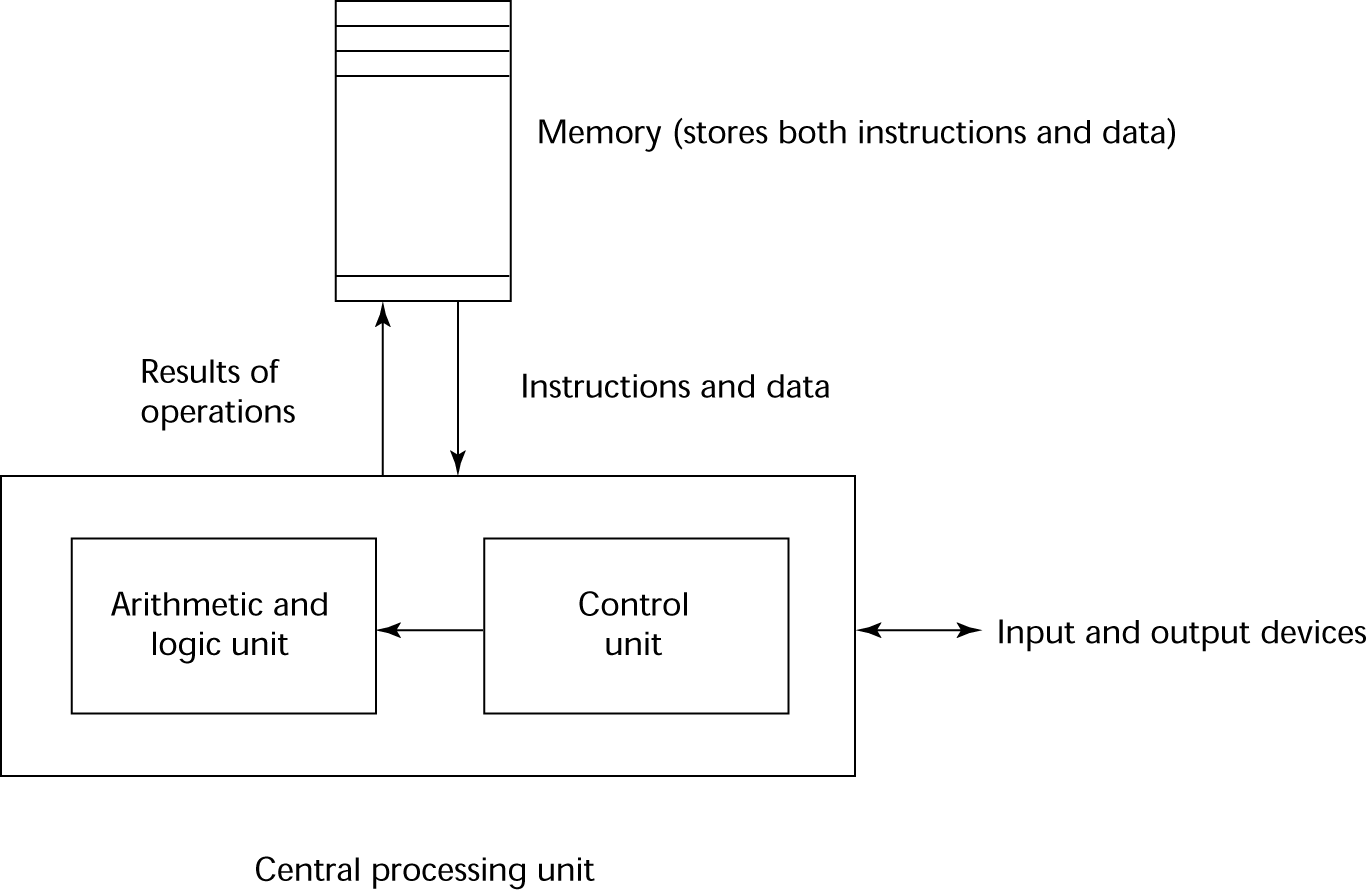
\includegraphics[width=\textwidth]{img/von_neumann.png}
		\caption{Architettura di Von Neumann.}
	\end{figure}

	\noindent
	Per operare su tali macchine, fu necessario inserire una CPU per eseguire algoritmi e operare sui dati in memoria. Il primo linguaggio che consente di programmare tale architettura è quello basato sull'implementazione dell'architettura stessa, ovvero la programmazione con schede perforate per esempio.\newpage
	
	\subsection{Definizioni}
	
	\subsubsection{Algoritmo}
	
	\begin{boxdef}
		Un \textcolor{Red3}{\textbf{algoritmo}} \textbf{è una sequenza finita di passi primitivi di calcolo descritti mediante una frase ben formata (programma) in un linguaggio di programmazione}.
	\end{boxdef}

	\noindent
	In altre parole, un algoritmo scompone un calcolo complesso in passi elementari di computazione. Esso è dunque un concetto astratto che trova la sua forma concreta in un programma che è la sequenza finita di istruzioni.\newline
	Data la definizione, è necessario precisare che:
	\begin{itemize}
		\item \textbf{Un programma non è necessariamente un algoritmo}, poiché una frase grammaticalmente corretta potrebbe non avere significato;
		\item \textbf{Lo stesso algoritmo può avere concretizzazioni diverse}, ovvero lo stesso algoritmo può essere implementato da infiniti programmi.
	\end{itemize}

	\longline

	\subsubsection{Dati}

	I programmi sono la concretizzazione degli algoritmi, i quali manipolano i \textcolor{Red3}{\textbf{dati}}. Essi sono informazioni memorizzate sia concretamente in celle di memoria, sia astrattamente in elementi che il linguaggio di programmazione può manipolare, ovvero le \textbf{variabili}.
	
	\longline
	
	\subsubsection{Sintassi e semantica}

	La trasformazione (scrittura) di un programma in un determinato linguaggio di programmazione rappresenta la \textcolor{Red3}{\textbf{sintassi}}, mentre l'effetto della sua esecuzione e la trasformazione dei dati eseguita, costituisce la \textcolor{Red3}{\textbf{semantica}}.\newpage
	
	\subsubsection{Linguaggio matematico e logico}
	
	Il \textcolor{Red3}{\textbf{linguaggio matematico}} è una notazione rigorosa per rappresentare funzioni, ma non sempre oggetti infiniti e computazioni, cioè passi di calcolo.\newline
	
	\noindent
	Il \textcolor{Red3}{\textbf{linguaggio logico}} sono regole e assiomi che rendono possibile specificare il processo di computazione, in modo implicito, e consente di rappresentare formalmente oggetti infiniti in modo finito, ma non computazioni infinite.
	
	\longline
	
	\subsubsection{Linguaggio di programmazione}
	
	\begin{boxdef}
		Un \textcolor{Red3}{\textbf{linguaggio di programmazione}} consente di specificare in modo accurato esattamente le primitive del processo di computazione, con la rigorosità e la potenza della logica.
	\end{boxdef}

	\longline
	
	\subsubsection{Programma}
	
	Un \textcolor{Red3}{\textbf{programma}} è un insieme finito di istruzioni e costrutti del linguaggio di programmazione.\newpage
		
	\subsection{Aspetti di progettazione}
	
	\subsubsection{Leggibilità}
	
	\begin{boxdef}
		La \textcolor{Red3}{\textbf{leggibilità}} (\emph{readability}) è la sintassi chiara, l'assenza di ambiguità, la facilità di lettura e la comprensione dei programmi.
	\end{boxdef}
	
	\noindent
	I fattori che contribuiscono alla leggibilità sono:
	\begin{enumerate}
		\item La \textbf{semplicità di un linguaggio}, per esempio pochi ed essenziali costrutti base. Infatti, un linguaggio inizia ad essere complicato quando per poter fare la stessa cosa si possono seguire molti percorsi diversi. Un altro fattore di complicazione è l'overloading degli operatori, ovvero quando il simbolo di un operatore ha molteplici significati.
		
		\item L'\textbf{ortogonalità} della progettazione di un linguaggio. Un elemento di un programma è ortogonale se è indipendente dal contesto di utilizzo all'interno di esso. Più un programma è ortogonale, meno eccezioni alla regola esistono.
		
		\item \textbf{Presenza di strumenti per la definizione di tipi di dati e strutture dati}. Ad esempio l'uso di booleani al posto dei valori interi.
		
		\item \textbf{Struttura della sintassi}, come parole chiave significative ad esempio.
	\end{enumerate}

	\longline
	
	\subsubsection{Scrivibilità}
	
	\begin{boxdef}
		La \textcolor{Red3}{\textbf{scrivibilità}} (\emph{writability}) è la facilita di utilizzo di un linguaggio per creare programmi, la facilità di analisi e la verifica dei programmi.
	\end{boxdef}
	
	\noindent
	I fattori che influenza la leggibilità sono gli stessi della scrivibilità.\newline
	
	\noindent
	In breve i fattori che che contribuiscono alla scrivibilità sono:
	\begin{enumerate}
		\item \textbf{Semplicità e ortogonalità}. La presenza di pochi costrutti consente al programmatore di conoscerli in gran parte e di sfruttare al massimo il linguaggio. Stessa cosa per il numero di primitive.
		
		\item \textbf{Supporto per l'astrazione}. La possibilità di utilizzare strutture o operazioni complesse in modi che permettono di ignorare i dettagli. Esistono due tipi di astrazione: processi e dati.
		
		\item \textbf{Espressività}. Si riferisce a molte caratteristiche, per esempio mettere a disposizione un insieme di modi relativamente convenienti per specificare operazioni.
	\end{enumerate}\newpage
	
	\subsubsection{Affidabilità e costo}
	
	\begin{boxdef}
		Per \textcolor{Red3}{\textbf{affidabilità}} (\emph{reliability}) si intende la conformità alle sue specifiche.
	\end{boxdef}
	\begin{boxdef}
		Per \textcolor{Red3}{\textbf{costo}} si intende letteralmente il costo complessivo di utilizzo.
	\end{boxdef}
	
	\noindent
	Un \textbf{programma} viene categorizzato come \textbf{affidabile} se soddisfa le seguenti condizioni:
	\begin{enumerate}
		\item \textbf{\emph{Type checking}}, ovvero il controllo degli errori di tipo. Viene eseguito spesso a tempo di compilazione poiché risulta costoso.
		
		\item \textbf{Gestione delle eccezzioni}. Gestire gli errori run-time per consentire la continuazione dell'esecuzione e l'attuazione di eventuali misure correttive.
		
		\item \textbf{Presenza di potenziali aliasing}. La presenza di due o più metodi di riferimento per la stessa locazione di memoria è un problema.
	\end{enumerate}

	\noindent
	Mentre le \textbf{specifiche di costo} riguardano:
	\begin{itemize}
		\item L'addestramento di programmatore per usare il linguaggio
		\item Scrittura di programma
		\item Compilazione dei programmi
		\item Esecuzione dei programmi
		\item Sistema di implementazione del linguaggio, ovvero la disponibilità di compilatori liberi
		\item Poca affidabilità fanno lievitare i costi
		\item Mantenimento dei programmi
	\end{itemize}\newpage

	\subsection{Classificazione dei linguaggi}
	
	I linguaggi possono essere classificati per: \textbf{metodo di computazione} e \textbf{per caratteristiche}.
	
	\longline
	
	\subsubsection{Metodo di computazione}
	
	I linguaggi possono essere a:
	\begin{itemize}
		\item \textcolor{Red3}{\textbf{Basso livello}}. Questi linguaggi hanno caratteristiche strettamente dipendente all'architettura su cui si sta programmando. Per esempio:
		\begin{itemize}
			\item Linguaggio binario che non fa distinzione tra dati e programmi;

			\item Assembly, linguaggio strutturato molto basso, vicino al linguaggio macchina.
		\end{itemize}
	
		\item \textcolor{Red3}{\textbf{Alto livello}}. Questi linguaggi consentono una programmazione strutturata in cui dati ed istruzioni hanno rappresentazioni diverse. Esistono tre tipi:
		\begin{itemize}
			\item \textcolor{Red3}{\textbf{Linguaggi imperativi}} che descrivono come \textbf{concetto chiave} l'elemento fondamentale dell'architettura di Von Neumann, ovvero la \textbf{cella di memoria}.\newline
			Il concetto di variabile rappresenta l'astrazione logica della cella.\newline
			Il concetto di assegnamento rappresenta l'operazione primitiva di modifica della cella di memoria e dunque dello stato della macchina.\newline
			Nei linguaggi imperativi, gli assegnamenti vengono controllati in modo sequenziale, condizionale e ripetuti.
			
			\item \textcolor{Red3}{\textbf{Linguaggi funzionali}} sono molto vicini alla matematica. Essi descrivono i passi di calcolo come funzioni matematiche. Il \emph{core} principale si concentra sulla composizione e applicazione di funzioni.\newline
			Una variabile viene intesa come un'incognita matematica e sostituita come se fosse un \emph{placeholder} all'interno del linguaggio. Infatti, essa \underline{non} può cambiare nel tempo durante la computazione.
			
			\item \textcolor{Red3}{\textbf{Linguaggi logici}} usano la logica, ovvero eseguono pattern matching. Come passo di calcolo primitivo utilizzano l'unificazione o la sostituzione.
		\end{itemize}
	\end{itemize}
	
	\longline

	\subsubsection{Per caratteristiche}
	
	La classificazione per caratteristiche è una metodologia utilizzata principalmente all'inizio dell'era informatica per studiare le caratteristiche di base quali: strutture di base di controllo, strutture per i dati, efficienze nell'esecuzione.\newline
	
	\noindent
	Andando avanti con il tempo, la classificazione si è focalizzata su caratteristiche aggiuntive, ovvero le strutture di base rimangono le stesse, ma ad esse vengono aggiunte nuove caratteristiche. In questo modo viene migliorata la soluziona di specifici problemi.\newpage
	
	\subsection{Implementazione dei linguaggi}
	
	L'\textbf{implementazione di un linguaggio} ha un collegamento stretto con il funzionamento della macchina su cui deve essere eseguito. Infatti, l'implementazione riguarda le metodologie per rendere comprensibile alla macchina da programmare il linguaggio scelto. Per farlo, è necessario introdurre il funzionamento di una macchina basata sull'architettura di Von Neumann. Essa si basa sulla ripetizione di un ciclo che costituisce l'\textbf{interprete} del linguaggio che la macchina riconosce:
	\begin{itemize}
		\item Lettura dell'istruzione dalla memoria (\emph{fetch})
		
		\item Decodifica dell'istruzione (\emph{decode})
		
		\item Lettura di eventuali operandi
		
		\item Memorizzazione ed esecuzione del risultato (\emph{exec})
	\end{itemize}
	\begin{figure}[!htp]
		\centering
		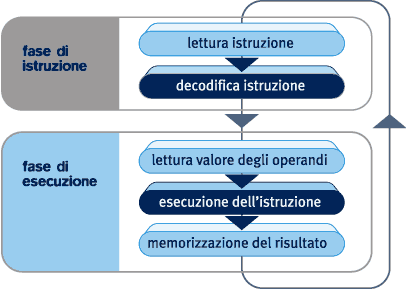
\includegraphics[width=.75\textwidth]{img/fasi_esecuzione.png}
		\caption{Ciclo di esecuzione delle istruzioni.}
	\end{figure}

	\longline\newpage

	\subsubsection{Macchina astratta}

	\noindent
	L'implementazione di un linguaggio \textbf{significa} considerare una macchina astratta poiché lavorando ad alto livello, le istruzioni vengono interpretate e dunque si ignorano momentaneamente il linguaggio binario e la macchina fisica.
	\begin{boxdef}
		Dato un linguaggio $L$ di programmazione, la \textcolor{Red3}{\textbf{macchina astratta}} $M_{L}$ per $L$ è un insieme di strutture dati ed algoritmi che permettono di memorizzare ed eseguire i programmi scritti in $L$.
	\end{boxdef}
	
	\noindent
	La collezione di strutture dati ed algoritmi è necessario per:
	\begin{itemize}
		\item Acquisire la prossima istruzione
		
		\item Gestire le chiamate e i ritorni dai sottoprogrammi
		
		\item Acquisire gli operandi e memorizzare i risultati delle operazioni
		
		\item Mantenere le associazioni fra nomi e valori denotati
		
		\item Gestire dinamicamente la memoria
	\end{itemize}

	\noindent
	In altre parole, una \textbf{macchina astratta} è la combinazione di una memoria che immagazzina i programmi e di un interprete che esegue istruzioni dei programmi.
	\begin{figure}[!htp]
		\centering
		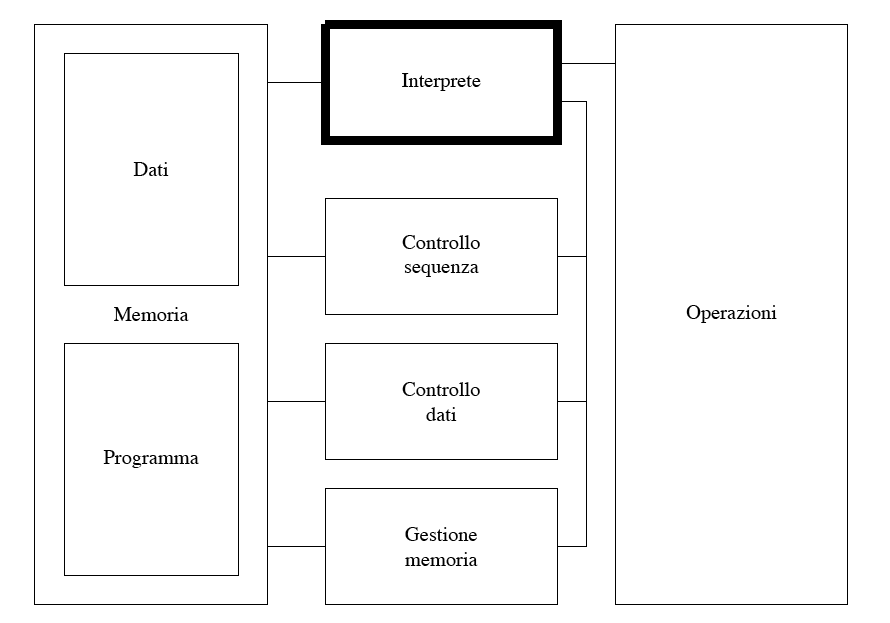
\includegraphics[width=\textwidth]{img/macchina_astratta.png}
		\caption{Rappresentazione di una macchina astratta.}
	\end{figure}
	
	\noindent
	Il \textbf{linguaggio} $L$ riconosciuto (interpretato) dalla macchina astratta $M_{L}$ viene chiamato \textbf{linguaggio macchina}. Formalmente, è l'insieme di tutte le stringhe interpretabili dalla macchina astratta $M$.\newpage
	
	\subsubsection{Realizzazione di una macchina astratta a vari livelli}
	
	Qualsiasi macchina astratta, per essere eseguita, deve prima o poi utilizzare qualche dispositivo hardware. Questo però non significa che tutte le macchine sono realizzate a livello hardware. Infatti, la realizzazione di una macchina astratta può avvenire tre categorie:
	\begin{itemize}
		\item \textcolor{Red3}{\textbf{Realizzazione hardware (HW)}}. Sempre possibile e concettualmente semplice. Il linguaggio macchina è il linguaggio fisico/binario e si realizza mediante dispositivi fisici. Data la sua lontananza dai linguaggi ad alto livello, la loro programmazione risulta complessa. Questo è uno dei tanti motivi per cui viene usata solo per sistemi dedicati.
		
		\item \textcolor{Red3}{\textbf{Realizzazione firmware (FW)}}. Le strutture dati e gli algoritmi vengono simulati nella macchina mediante microprogrammi. Il linguaggio macchina è a basso livello e consiste in microistruzioni che specificano le operazioni di trasferimento dati tra registri. Il vantaggio è dato dalla velocità e la flessibilità maggiore rispetto all'hardware.
		
		\item \textcolor{Red3}{\textbf{Realizzazione software (SW)}}. Le strutture dati e gli algoritmi vengono realizzati tramite un linguaggio implementato. In questo modo è possibile scrivere programmi che interpretano i costrutti del linguaggio macchina simulando le funzionalità della macchina. La velocità viene diminuita ma aumenta molto la flessibilità.
	\end{itemize}\newpage

	\subsubsection{Realizzazione software e livelli di astrazione}
	
	Con la realizzazione software, vengono utilizzati linguaggi di programmazione ad alto livello poiché essi implementano una struttura suddivisa a livelli di astrazione. Ogni livello coopera in modo sequenziale ma allo stesso tempo è indipendente.
	
	\begin{figure}[!htp]
		\centering
		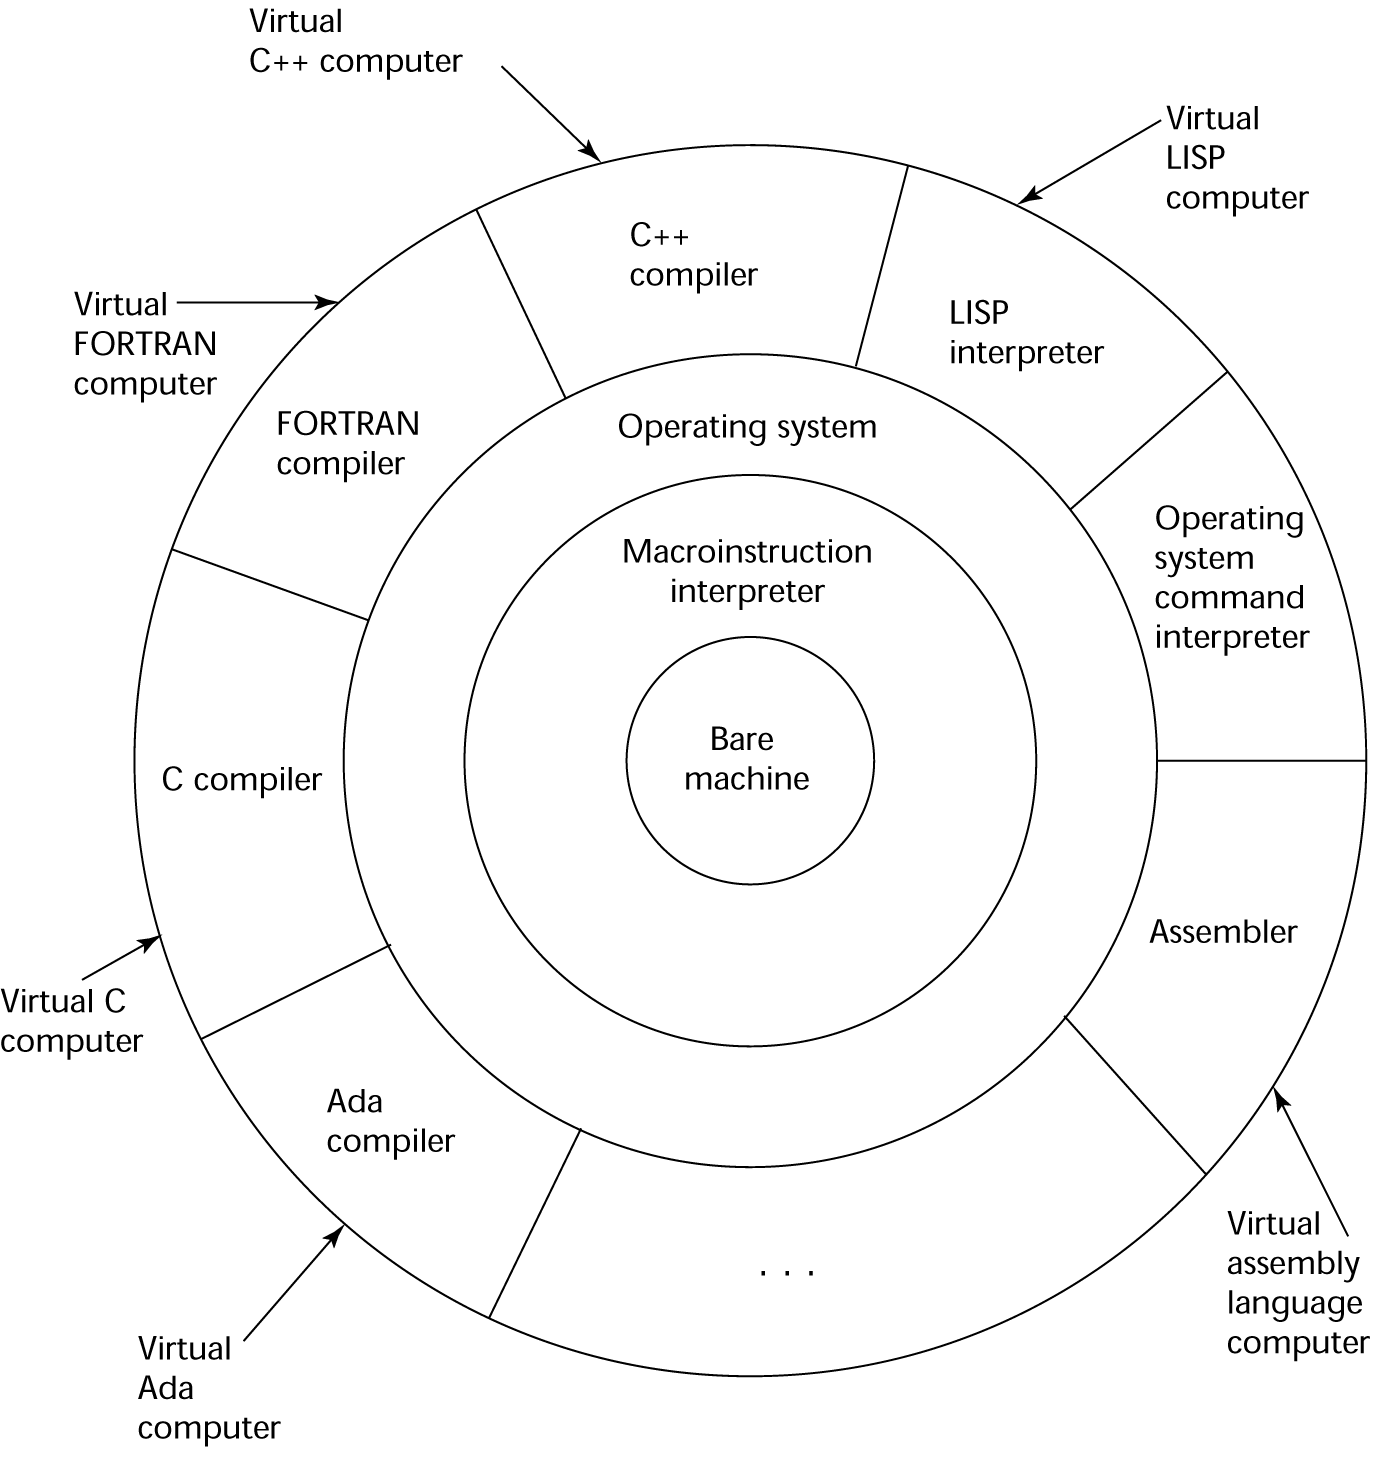
\includegraphics[width=.8\textwidth]{img/astrazione.png}
		\caption{Livelli di astrazione utilizzati dai linguaggi ad alto livello.}
	\end{figure}

	\noindent
	Quindi, la macchina può essere vista come una stratificazione di livelli di astrazione:
	\begin{figure}[!htp]
		\centering
		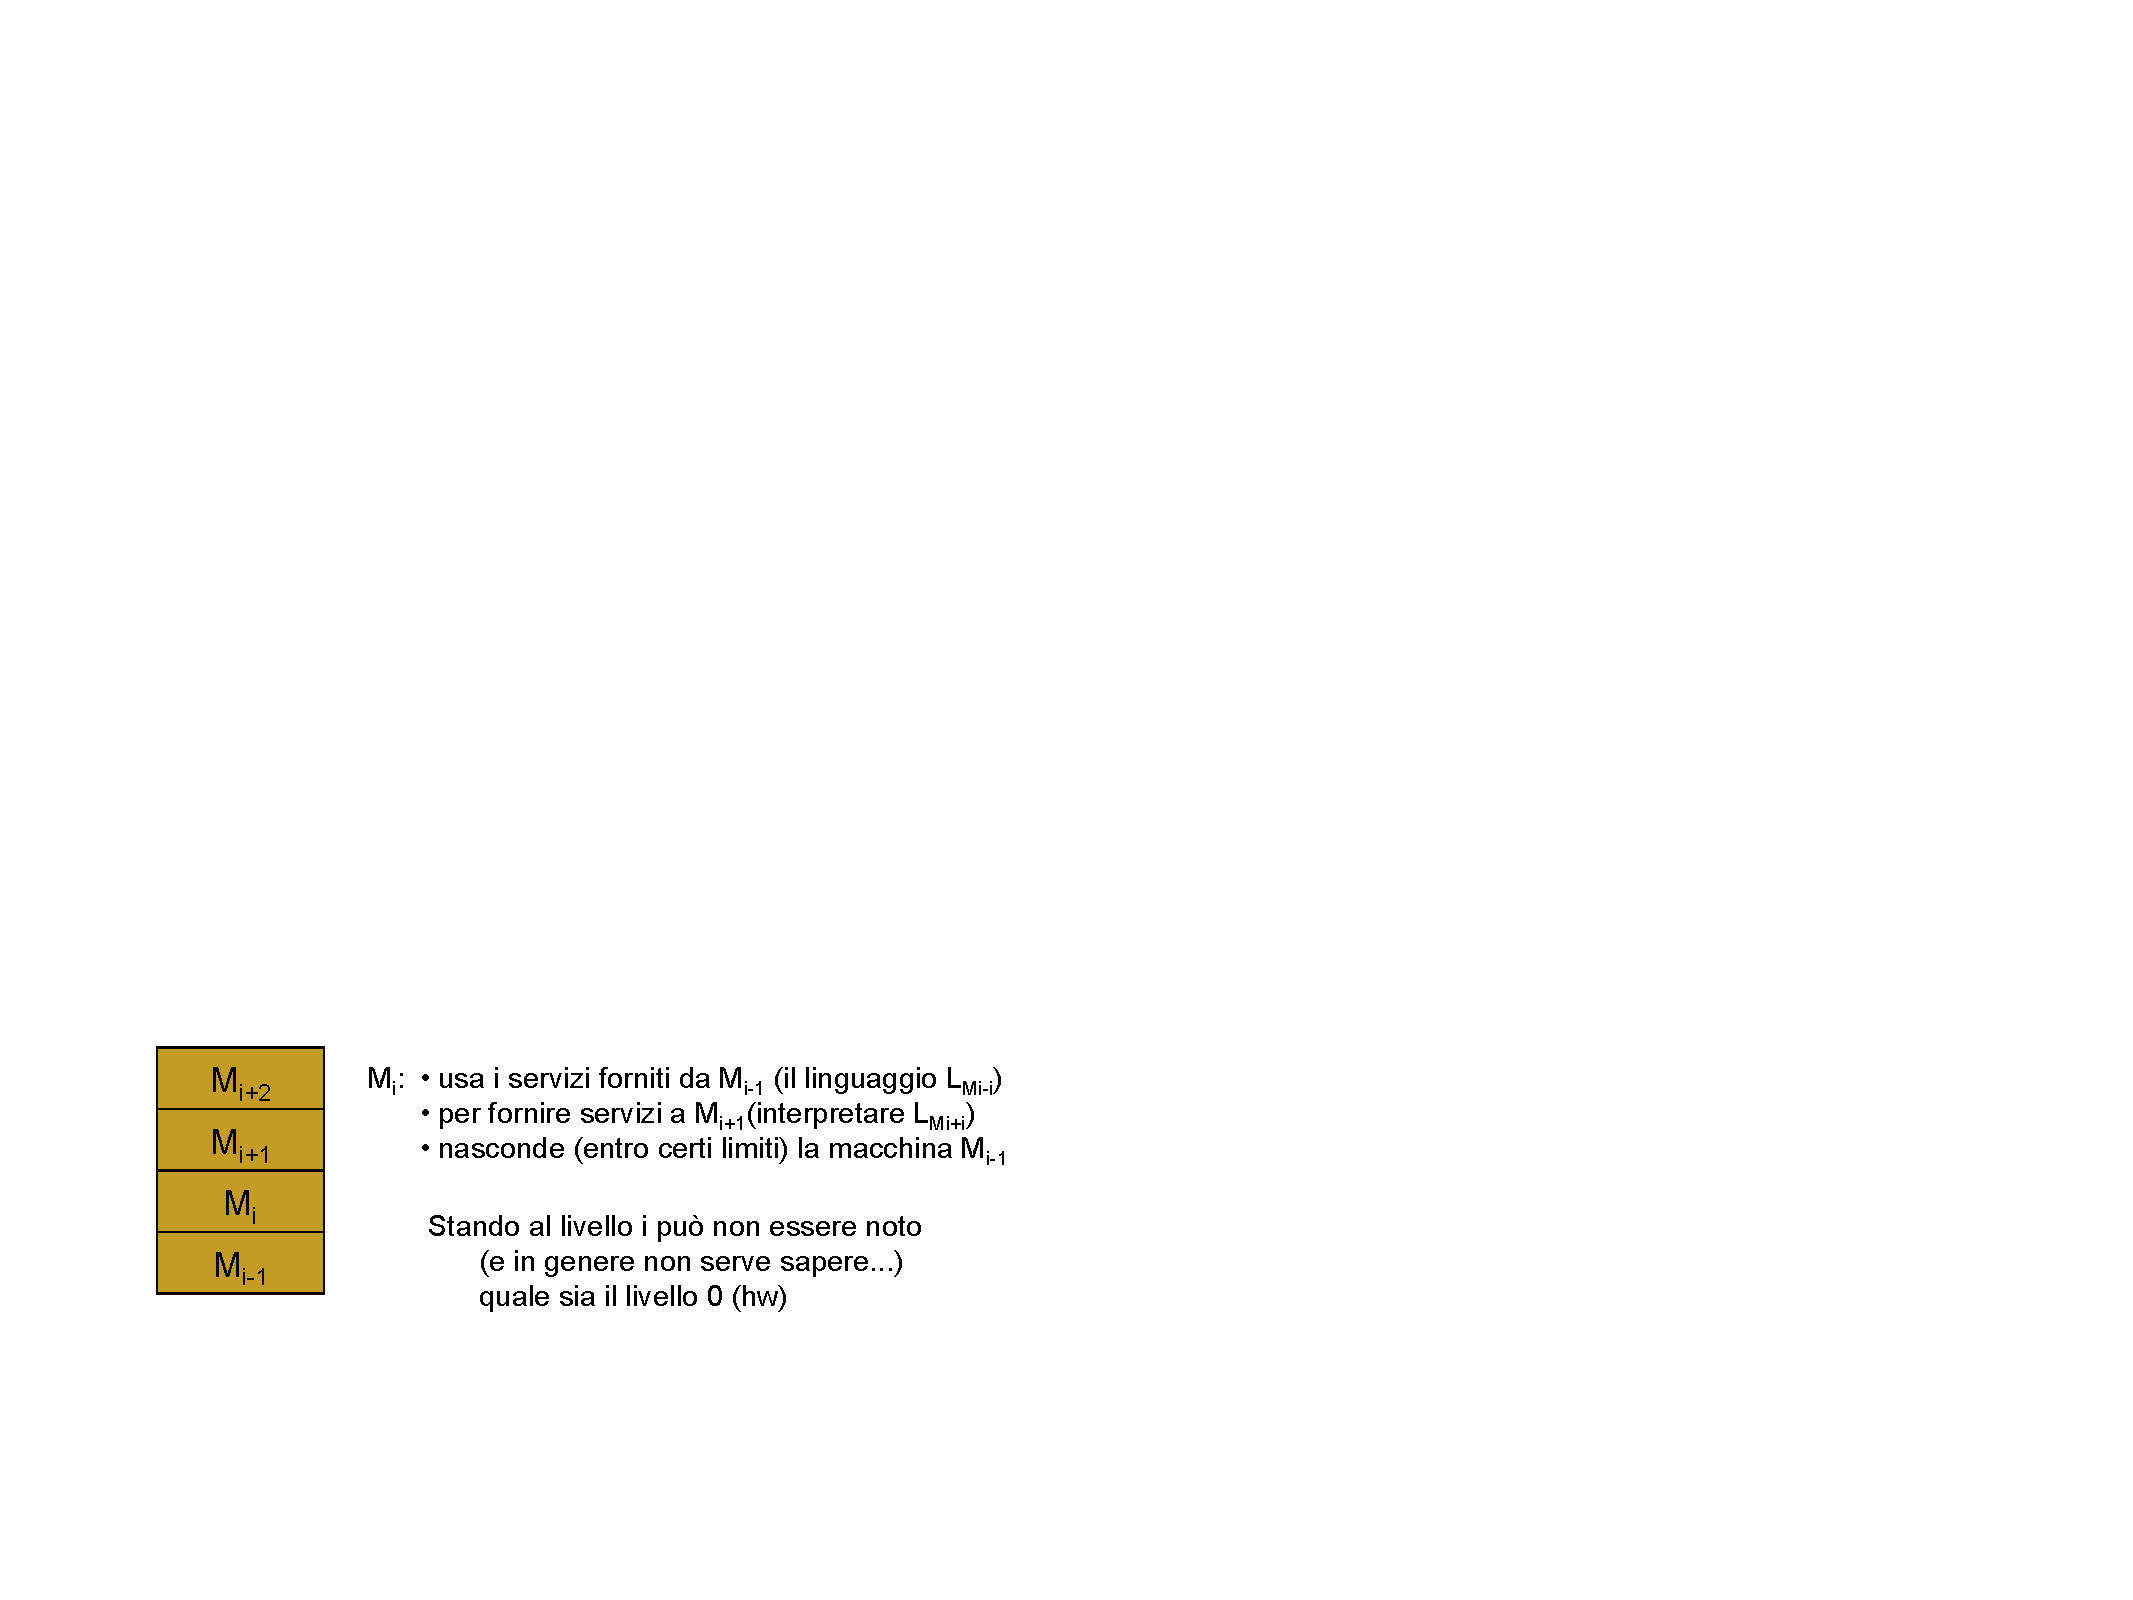
\includegraphics[width=.8\textwidth]{img/livelli_astrazione_macchina.pdf}
	\end{figure}\newpage

	\subsection{Realizzazione di una macchina a livello software/firmware}
	
	Sia $L$ un linguaggio da implementare e sia $M_{L_{0}}$ una macchina astratta a disposizione che ha come linguaggio macchina $L_{0}$. La macchina astratta $M_{L_{0}}$ è il livello su cui si vuole implementare il linguaggio $L$ e che mettette a disposizione di $M_{L}$ le sue funzionalità.\newline
	
	\noindent
	Dunque, la realizzazione di una macchina astratta $M_{L}$ consiste nel realizzare una macchina che \dquotes{traduce} il linguaggio $L$ (ad alto livello per esempio) in linguaggio macchina $L_{0}$, ovvero che interpreta tutte le istruzioni di $L$ come istruzioni di $L_{0}$. La traduzione avviene tramite due metodi a scelta:
	\begin{itemize}
		\item \textbf{Soluzione interpretativa}. Simulazione dei costrutti della macchina astratta $M_{L}$ da realizzare, mediante programmi scritti in $L_{0}$;
		\item \textbf{Soluzione compilativa}. Traduzione esplicita dei programmi di $L$ in corrispondenti programmi di $L_{0}$.
	\end{itemize}\newpage

	\subsubsection{Soluzione interpretativa: interprete}\label{interprete}
	
	La soluzione interpretativa prevede l'utilizzo di un interprete per la realizzazione di una macchina astratta. Un \textcolor{Red3}{\textbf{interprete}} è un programma $\mathrm{int}^{\mathrm{L_{0}, L}}$ che esegue, sulla macchina astratta per $L_{0}$, programmi $P^{L}$, scritti nel linguaggio di programmazione $L$, su un input fissato appartenente all'insieme di dati (input e output). In breve, un interprete è una \textbf{macchina universale} che preso un programma e un suo input, lo esegue su quell'input usando solo funzionalità messe a disposizione dal livello (macchina astratta) sottostante.
	\begin{boxdef}
		\begin{center}
			\textcolor{Red3}{\textbf{\emph{Notazioni}}}
		\end{center}
		\begin{itemize}
			\item $Prog^{L}$ è l'insieme di programmi scritti nel linguaggio di programmazione $L$;
			\item $D$ è l'insieme di dati, ovvero input e output;
			\item $P^{L}$ è il programma scritto nel linguaggio di programmazione $L$;
			\item Relazioni ovvie: $P^{L} \in Prog^{L}$ e $in, out \in D$;
			\item $\exec{P^{L}}: D \longrightarrow D$ è la notazione utilizzata per indicare che l'esecuzione del programma scritto nel linguaggio di programmazione $L$ con input $in$ è uguale all'output $out$. Quindi $\exec{P^{L}}\left(in\right) = out$.
		\end{itemize}
	\end{boxdef}
	\begin{boxdef}
		Un \textcolor{Red3}{\textbf{interprete formalmente}} è esprimibile nel seguente modo.\newline
		Si consideri un interprete da $L$ a $L_{0}$: dato $P^{L} \in Prog^{L}$ e $in \in D$, un interprete $int^{L, L_{0}}$ per $L$ su $L_{0}$ è un programma tale che:
		\begin{equation*}
			\exec{int^{L, L_{0}}}: \left(Prog^{L}\right) \longrightarrow D
		\end{equation*}
		e dunque:
		\begin{equation*}
			\exec{int^{L, L_{0}}}\left(P^{L}, in\right) = \exec{P^{L}}\left(in\right)
		\end{equation*}
	\end{boxdef}
	
	\noindent
	Anche un programma può essere utilizzato come dato di input in un altro programma. Si osservi il seguente diagramma:
	\begin{figure}[!htp]
		\centering
		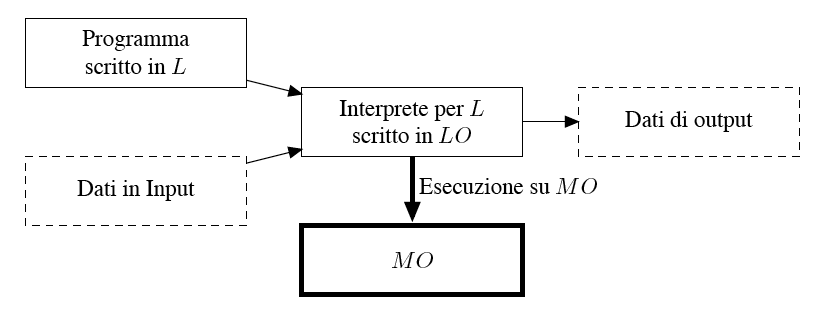
\includegraphics[width=\textwidth]{img/programma_input.png}
	\end{figure}
	
	\noindent
	Si noti come un programma scritto nel linguaggio $L$, insieme ad eventuali altri input, viene interpretato da un programma creato appositamente per eseguire questo compito su $L$, ma scritto in $L_{0}$. L'\textbf{esecuzione comporta una decodifica e non una traduzione esplicita}. Infatti, l'interprete simula ogni istruzione di $L$ utilizzando un certo insieme di istruzioni di $L_{0}$. Questa è la base dei linguaggi di scripting.
		
	\longline
	
	\subsubsection{Soluzione interpretativa: operazioni e struttura}
	
	Un interprete può eseguire una serie di \textbf{operazioni}:
	\begin{itemize}
		\item \textcolor{Red3}{\textbf{Elaborazione dei dati primitivi}}. I dati primitivi sono dati rappresentabili in modo diretto nella memoria, per esempio i numeri. Le elaborazioni di essi, sono implementate direttamente nella struttura della macchina;
		
		\item \textcolor{Red3}{\textbf{Controllo di sequenza delle esecuzioni}}. Non è altro che la gestione del flusso di esecuzione delle istruzioni, le quali non sempre sono sequenziali, tramite alcune strutture dati;
		
		\item \textcolor{Red3}{\textbf{Controllo dei dati}}. Recupero dei dati necessari per eseguire le istruzioni. I dati possono riguardare le modalità di indirizzamento della memoria e l'ordine con cui recuperare gli operandi;
		
		\item \textcolor{Red3}{\textbf{Controllo della memoria}}. È necessaria una gestione della memoria per allocare dati e programmi. Cambia a seconda del tipo di realizzazione della macchina astratta:
		\begin{itemize}
			\item Realizzazione hardware (HW): la gestione è semplice poiché nella peggiore delle ipotesi, i dati potrebbero essere rimasti sempre nelle stesse locazioni.
			
			\item Realizzazione software (SW): la gestione è complessa ed esistono costrutti di allocazione e deallocazione che richiedono alcune strutture dati (e.g. pile) e operazioni dinamiche.
		\end{itemize}
	\end{itemize}
	Date le operazioni elencate, il \textcolor{Red3}{\textbf{ciclo di esecuzione di un interprete}} è il seguente:
	\begin{lstlisting}[language=C]
begin
	go := true;
	while go do begin
		FETCH(OPCODE, OPINFO) at PC
		DECODE(OPCODE, OPINFO)
		if OPCODE needs ARGS then FETCH (ARGS)
		case OPCODE of
			OP1: EXECUTE(OP1, ARGS)
			...
			OPn: EXECUTE(OPn, ARGS)
			HLT: go := false;
		if OPCODE has result then STORE(RES);
		PC := PC + SIZE(OPCODE);
	end
end \end{lstlisting}
	\begin{itemize}
		\item Righe 1-3: finché \textsf{go} ha il valore \textsf{true}, il codice viene eseguito;
		\item Riga 4: estrazione dell'istruzione riferita ad \textsf{OPCODE} (controllo sequenza 1 su 2);
		\item Righe 5: decodifica dell'istruzione estratta alla riga precedente;
		\item Riga 6: prelievo dalla memoria gli operandi richiesti da \textsf{OPCODE} e nelle modalità individuate (controllo dati 1 su 2);
		\item Righe 7-11: esecuzione delle operazioni;
		\item Riga 12: se l'operazione ha un risultato da salvare, allora viene salvato in memoria (controllo dati 2 su 2);
		\item Riga 13: viene incrementato il \emph{program counter} (PC) per eseguire la prossima istruzione (controllo sequenza 2 su 2).
	\end{itemize}
	Il ciclo continua ad essere eseguito finché la variabile \textsf{go} ha valore \textsf{true}. Inoltre, le istruzioni riferite al program counter sono chiamate istruzioni di \textbf{controllo sequenza} (CS) perché manipolano e accedono al program counter. Mentre le operazioni di memorizzazione/estrazione sugli argomenti si chiamano \textbf{controllo dati} (CD).
	\begin{figure}[!htp]
		\centering
		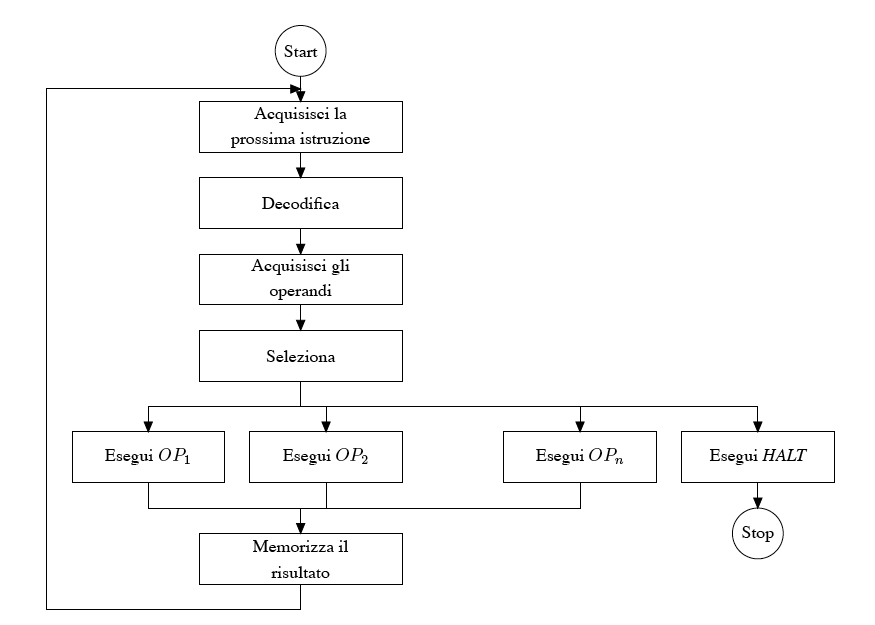
\includegraphics[width=\textwidth]{img/ciclo_esecuzione_interprete.png}
		\caption{Diagramma a blocchi della struttura di un interprete.}
	\end{figure}\newpage

	\subsubsection{Soluzione interpretativa: pro e contro}
	
	\begin{itemize}
		\item \textcolor{Green4}{\textbf{Pro:}}
		\begin{itemize}
			\item \textbf{Facilità di interazione \emph{run-time}}. Interpretazione al momento dell'esecuzione consente di interagire direttamente con l'esecuzione del programma (\emph{debugging});
			\item Velocità nello sviluppo applicativo di un interprete, quindi \textbf{tempi ridotti per la sua creazione};
			\item Utilizzo della \textbf{memoria ridotto} rispetto ad un compilatore.
		\end{itemize}

		\item \textcolor{Red3}{\textbf{Contro:}}
		\begin{itemize}
			\item Tempi di decodifica sommati a quelli d'esecuzione ogni volta che un'istruzione viene eseguita, si traduce in un'\textbf{esecuzione lenta} e quindi una scarsa efficienza della macchina.
		\end{itemize}
	\end{itemize}\newpage
	
	\subsubsection{Soluzione compilativa: compilatore}\label{compilatore}

	Un \textcolor{Red3}{\textbf{compilatore}} è un programma $\mathrm{comp}^{L_{0}, L}$ che \textbf{traduce}, preservando semantica e funzionalità, programmi scritti nel linguaggio di programmazione $L$ in programmi scritti in $L_{0}$, e quindi eseguibili direttamente sulla macchina astratta per $L_{0}$.
	Come l'interprete, anche il compilatore accetta un programma come input poiché viene considerato come dato.\newline
	
	\noindent
	\begin{boxdef}
		\begin{center}
			\textcolor{Red3}{\textbf{\emph{Notazioni}}}
		\end{center}
		\begin{itemize}
			\item $Prog^{L}$ è l'insieme di programmi scritti nel linguaggio di programmazione $L$;
			\item $D$ è l'insieme di dati, ovvero input e output;
			\item $P^{L}$ è il programma scritto nel linguaggio di programmazione $L$;
			\item Relazioni ovvie: $P^{L} \in Prog^{L}$ e $in, out \in D$;
			\item $\exec{P^{L}}: D \longrightarrow D$ rappresenta la semantica di $P^{L}$.
		\end{itemize}
	\end{boxdef}\:\newline

	\noindent
	\begin{boxdef}
		Un \textcolor{Red3}{\textbf{compilatore formalmente}} è esprimibile nel seguente modo.\newline
		Dato $P^{L} \in Prog^{L}$, un \textbf{compilatore} $\mathrm{comp}^{L, L_{0}}$ da $L$ a $L_{0}$ è un programma tale che:
		\begin{equation*}
			\exec{comp^{L, L_{0}}}: Progr^{L} \longrightarrow Progr^{L_{0}}
		\end{equation*}
		e dunque:
		\begin{equation*}
			\exec{comp^{L, L_{0}}}\left(P^{L}\right) = P^{L_{0}} \text{ tale che } \forall in \in D. \exec{P^{L_{0}}}\left(in\right) = \exec{P^{L}}\left(in\right)
		\end{equation*}
	\end{boxdef}\:\newline
	
	\noindent
	Ovvero che l'esecuzione della compilazione del linguaggio $L$ a $L_{0}$ con input il programma scritto in $L$, l'output sia uguale al programma scritto nel linguaggio $L_{0}$; tale che per ogni input appartenente all'insieme dei dati, l'esecuzione del programma scritto in $L_{0}$ con input $in$, sia uguale all'esecuzione del programma scritto in $L$ con input $in$.\newpage

	\noindent
	Con un compilatore, la \textbf{traduzione} è \textbf{esplicita} poiché il codice in $L$ viene prodotto come output e non eseguito. Quindi, per eseguire il programma $P^{L}$ con input $in$, è necessario prima eseguire $comp^{L, L_{0}}$ con $P^{L}$ come input.
	L'esecuzione avverrà sulla macchina astratta $M_{A}$ del linguaggio in cui è scritto il compilatore. Il risultato dunque è un altro programma (compilato) $P^{L_{0}}$, scritto in $L_{0}$. Solo a questo punto è possibile eseguire $P^{L_{0}}$ su $M_{L_{0}}$ con input $in$.
	Un \textbf{esempio} di linguaggio compilato è il C.
	\begin{figure}[!htp]
		\centering
		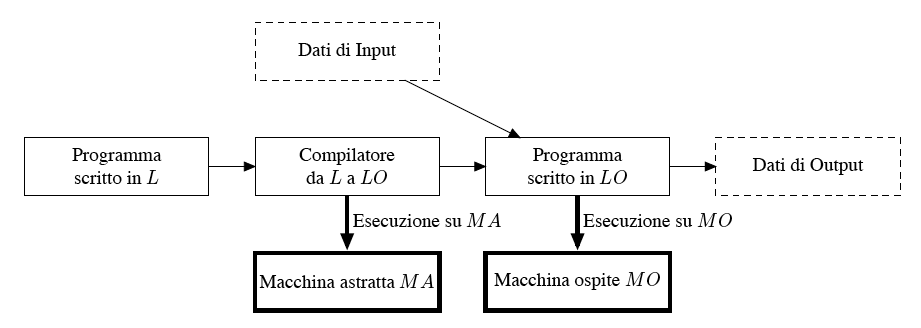
\includegraphics[width=\textwidth]{img/compilatore.png}
	\end{figure}\newpage

	\subsubsection{Soluzione compilativa: struttura}

	La compilazione deve tradurre un programma da un linguaggio ad un altro preservandone la semantica: si deve avere la certezza che il programma compilato faccia esattamente quello che faceva il sorgente. L'\textcolor{Red3}{\textbf{esecuzione}} di un compilatore si articola in varie fasi:
	\begin{figure}[!htp]
		\centering
		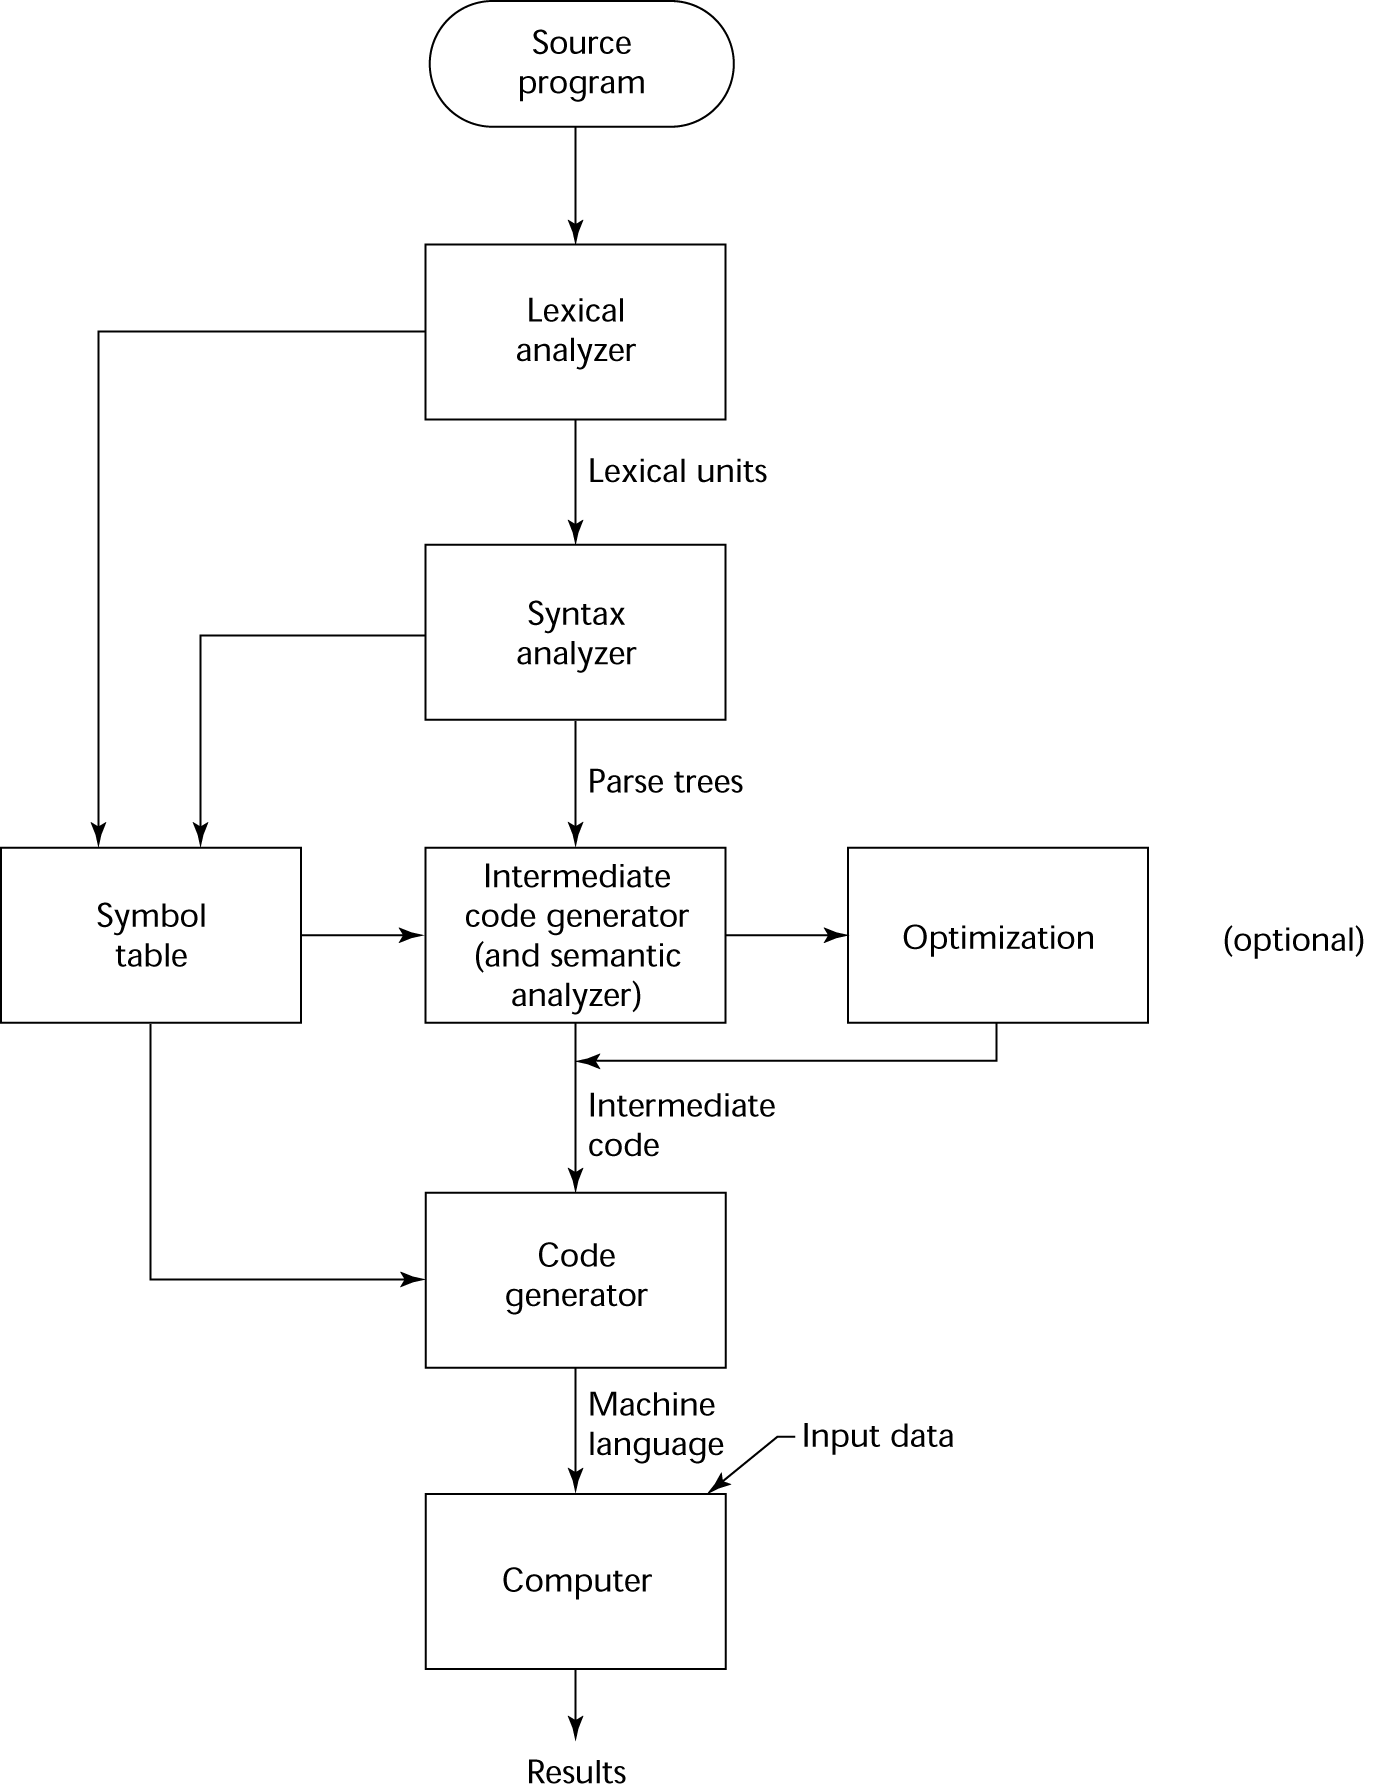
\includegraphics[width=.85\textwidth]{img/fasi_compilatore.png}
	\end{figure}
	
	\begin{itemize}
		\item \textcolor{Red3}{\textbf{Analisi lessicale}} (\emph{Lexical analyzer}), divide il programma in componenti sintattici primitivi chiamati \textbf{tokens} (identificatori, numeri, parole riservate). I \emph{tokens} sono coloro che formano i linguaggi regolari.\newline
		In altre parole, l'\textbf{analisi lessicale converte caratteri del programma sorgente in unità lessicali};\newpage

		\item \textcolor{Red3}{\textbf{Analisi sintattica}} (\emph{Syntax analyzer}), crea una rappresentazione ad albero della sintassi del programma. Ogni foglia è un \emph{token} e le foglie lette da sinistra verso destra costituiscono frasi ben formate del linguaggio. Inoltre, l'albero costituisce la struttura logica del programma e dunque nel momento in cui non fosse possibile costruire l'albero, significherebbe che qualche frase è illegale. Questo genere di evento si traduce in un errore di compilazione. Le frasi di token formano linguaggi CF.\newline
		In altre parole, l'\textbf{analisi sintattica trasforma unità lessicali in \emph{parse tree} che rappresentano la struttura sintattica del programma}.

		\item \textcolor{Red3}{\textbf{Tabella dei simboli}} (\emph{Symbol table}), memorizza le informazioni sui nomi presente nel programma, come gli identificatori, le chiamate di procedura, ecc.
		
		\item \textcolor{Red3}{\textbf{Analisi semantica}} (\emph{Semantic analyzer}), consente di rilevare errori semantici, grazie all'analisi semantica, e di generare codice intermedio che ha la caratteristica di essere indipendente dall'architettura (compito del \emph{Intermediate code generator}).

		\item \textcolor{Red3}{\textbf{Ottimizzazione}} (\emph{Optimization}), opzionale, consente di ottimizzare il codice.

		\item \textcolor{Red3}{\textbf{Generatore di codice}} (\emph{Code generator}), viene generato codice macchina che ha la caratteristica di essere dipendente dall'architettura.
	\end{itemize}

	\longline

	\subsubsection{Soluzione compilativa: pro e contro}
	
	\begin{itemize}
		\item \textcolor{Green4}{\textbf{Pro:}}
		\begin{itemize}
			\item \textbf{Esecuzione molto efficiente}, il codice viene anche ottimizzato;
		\end{itemize}

		\item \textcolor{Red3}{\textbf{Contro:}}
		\begin{itemize}
			\item \textbf{Interazione \emph{run-time} molto difficile};
			\item Un \textbf{errore} a \emph{run-time} è \textbf{difficile da associare} all'esatto comando del codice sorgente (debugging complesso);
		\end{itemize}
	\end{itemize}\newpage

	\subsubsection{Soluzione reale: ibrido}\label{ibrido}

	Nella realtà esiste un compromesso tra compilatore e interprete. Ovvero, una \textcolor{Red3}{\textbf{soluzione ibrida}} dove il linguaggio
	ad alto livello viene compilato in un linguaggio a più basso livello che poi viene interpretato.
	\begin{figure}[!htp]
		\centering
		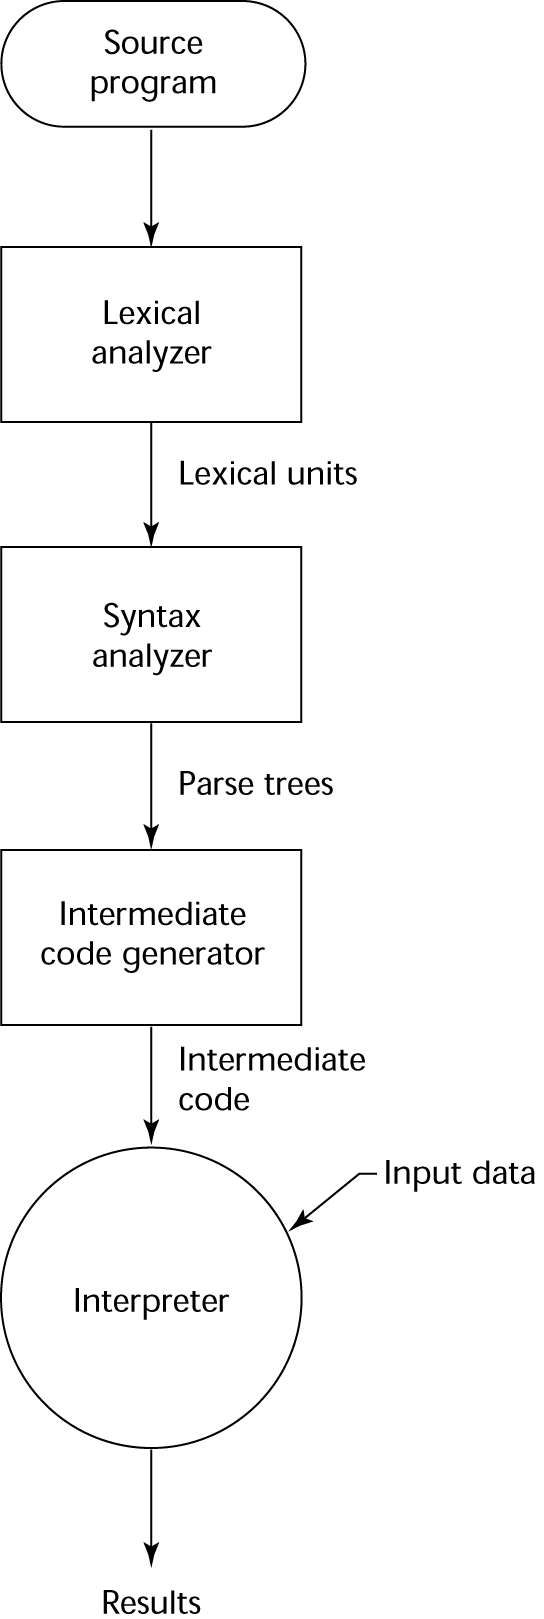
\includegraphics[width=.3\textwidth]{img/soluzione_reale_ibrida.png}
	\end{figure}

	\noindent
	Il \textbf{procedimento} è il seguente.\newline
	Si consideri il linguaggio ad alto livello $L$ per il quale si deve realizzare la macchina astratta $M_{L}$.\newline
	Il linguaggio $L$ viene quindi tradotto in un linguaggio intermedio $L_{Mi}$ la cui macchina astratta $M_{I}$ consiste in un interprete del linguaggio $L_{Mi}$ sulla macchina ospite $M_{O}$.\newline

	\noindent
	La separazione non è netta poiché vengono interpretati i costrutti lontani da $M_{O}$, mentre viene compilato il resto. Il passaggio chiave è la traduzione (compilazione) da $L$ ad un linguaggio intermedio (quello interpretato). Questo accade spesso nella realtà, specialmente con le \emph{system call} del sistema operativo. In parole povere, si cerca di trovare una connessione a metà strada.\newpage
	\begin{figure}[!htp]
		\centering
		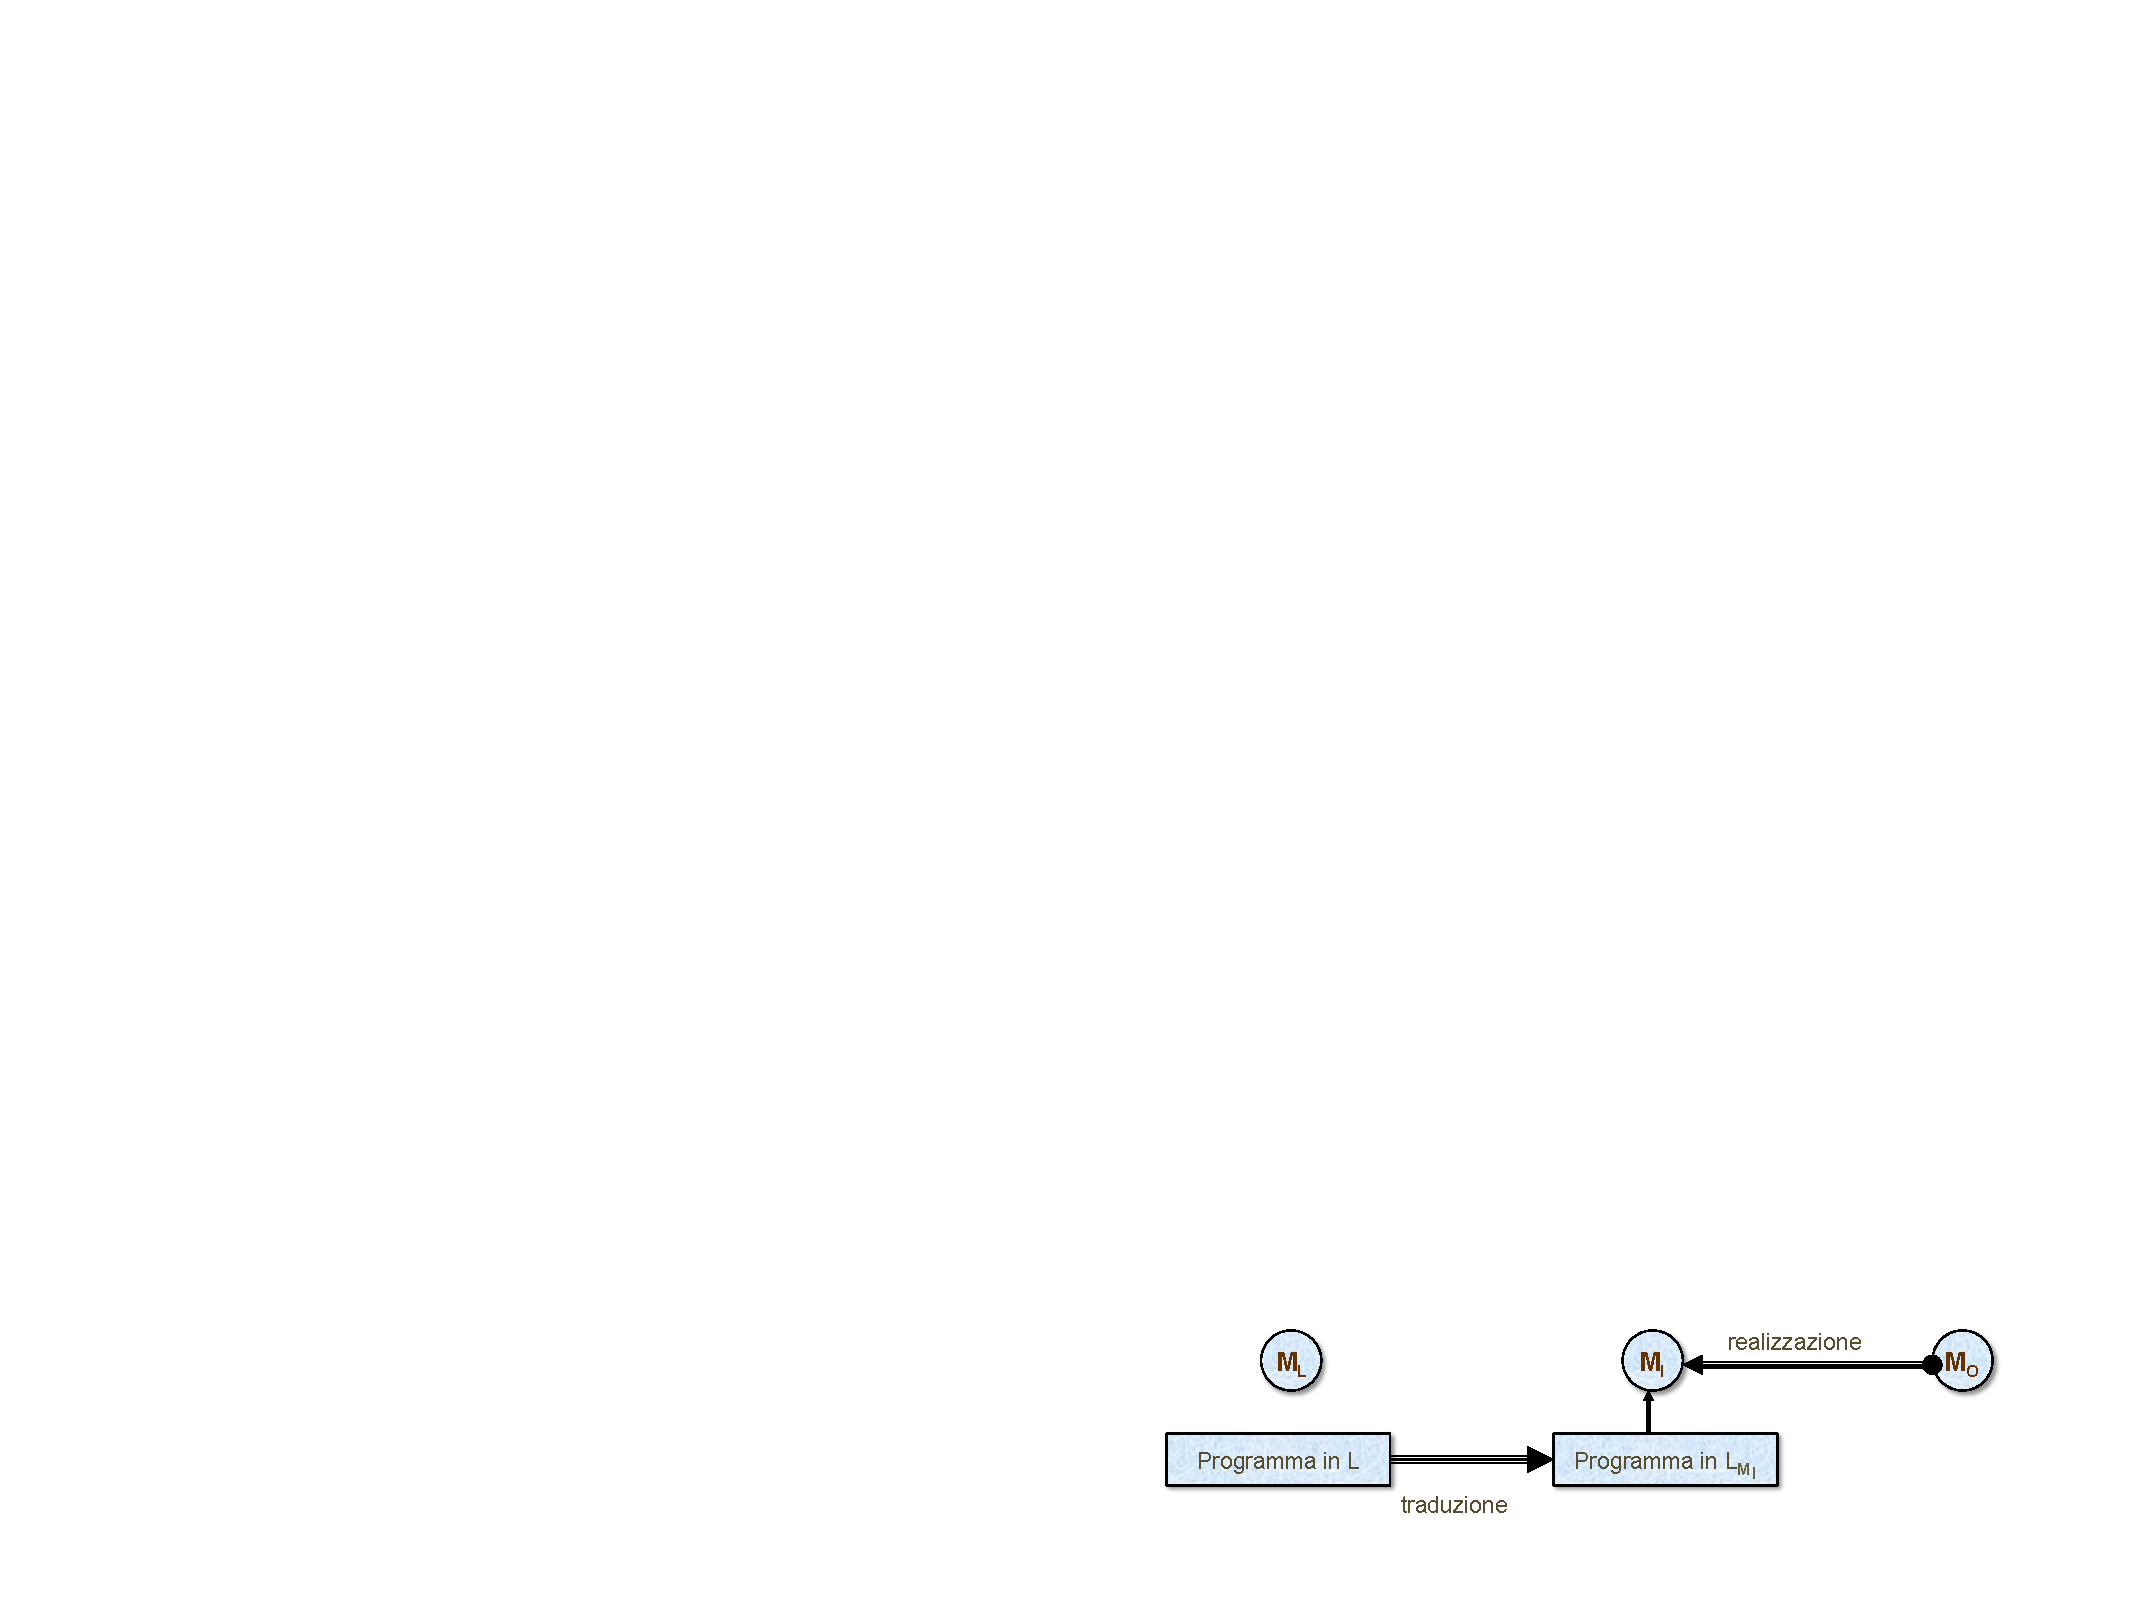
\includegraphics[width=\textwidth]{img/soluzione_ibrida_system_call.pdf}
		\caption{Soluzione ibrida con le \emph{system call}.}
	\end{figure}

	\longline

	\subsection{Sintesi}

	Nell'evoluzione dei linguaggi di programmazione, esistono fondamentalmente tre situazioni possibili:
	\begin{itemize}
		\item \textcolor{Red3}{\textbf{Interprete puro}} (paragrafo \ref{interprete}), $M_{L} = M_{I}$ (interprete per $L$ realizzato sulla macchina ospite $M_{O}$). Per esempio i linguaggi logici e funzionali, e di scripting (JS, PHP, ...)

		\item \textcolor{Red3}{\textbf{Compilatore}} (paragrafo \ref{compilatore}), macchina intermedia $M_{I}$ realizzata per estensione sulla macchina ospite $M_{O}$. Per esempio i linguaggi imperativi come C, C++, Pascal
		
		\item \textcolor{Red3}{\textbf{Implementazione mista}} (paragrafo \ref{ibrido}), traduzione dei programmi da $L$ ad un linguaggio intermedio $L_{Mi}$. I programmi $L_{Mi}$ sono poi interpretati sulla macchina ospite $M_{O}$. Per esempio, Java con il suo linguaggio intermedio Java bytecode, Pascal con il suo linguaggio intermedio P-code.
	\end{itemize}\newpage

	\section{Descrivere i linguaggi}

	Un \textbf{linguaggio di programmazione} è un linguaggio naturale, ma con alcune semplificazioni e \textbf{non ambiguo}. Quindi, per descriverli è necessario affrontare alcune tematiche:
	\begin{itemize}
		\item Grammatica, o meglio la \textcolor{Red3}{\textbf{sintassi}}: costituisce l'\textbf{insieme delle regole che consentono di costruire frasi corrette}. Viene quindi individuato l'alfabeto con cui sono costruite le frasi, le parole che compongono le frasi e infine viene eseguito un controllo della grammatica per verificare se le frasi le rispettano (il compito di verificare è assegnato al \textbf{\emph{parsing}});
		\item \textcolor{Red3}{\textbf{Semantica}}: nei linguaggi rappresenta la \textbf{relazione tra segni} (frasi legali) \textbf{e significati} (entità autonome che esistono indipendentemente dai segni utilizzati). Per esempio, la semantica di un programma può essere la funzione matematica calcolata dal programma. Solitamente la semantica viene specificata descrivendo gli effetti della sintassi su una rappresentazione astratta della macchina, chiamata \textbf{stato};
		\item \textcolor{Red3}{\textbf{Pragmatica}}: analisi delle \textbf{frasi che hanno lo stesso significato, ma possono essere utilizzate diversamente} in modo dipendente dal contesto linguistico;
		\item \textcolor{Red3}{\textbf{Implementazione}}: aspetti riguardanti la tecnica di implementazione utilizzata, i vincoli dell'architettura o della macchina, l'interfaccia del sistema operativo, gestione degli errori.\newline
		In sintesi, sono tutti gli aspetti che hanno effetto sul funzionamento del linguaggio ma che dipendono dalla macchina su cui esso viene eseguito.
	\end{itemize}\newpage

	\subsection{Sintassi}

	\subsubsection{Definizione e notazione}

	Le regole sintattiche (\textcolor{Red3}{\textbf{sintassi}}) del linguaggio specificano quali stringhe di caratteri sono legali nel linguaggio.\newline
	
	\noindent
	La terminologia linguistica utilizzata è la seguente:
	\begin{itemize}
		\item Una \textbf{parola} è una stringa di caratteri su un alfabeto;
		\item Una \textbf{frase} è una sequenza, ben formata, di parole;
		\item Una \textbf{linguaggio} è un insieme di frasi.
	\end{itemize}
	Invece, la \textbf{terminologia tecnica} utilizzata nel mondo dell'informatica è la seguente:
	\begin{itemize}
		\item Le \textbf{parole} vengono chiamate \textcolor{Red3}{\textbf{lessemi}}. Un lessema è una \textbf{parola con un significato specifico}, nella grammatica corrisponde ad un terminale. Rappresenta anche l'\textbf{unità minima sintattica}, ovvero quella a più basso livello di un linguaggio di programmazione (e.g. \textsf{begin}). \textbf{Per esempio}, in $index = 2$, sia $index$, $=$, che $2$ sono lessemi;
		\item Le \textbf{frasi} vengono chiamate \textcolor{Red3}{\textbf{\emph{token}}}. Essi corrispondono agli elementi delle categorie sintattiche del linguaggio di programmazione, e nella grammatica corrispondono alle sequenze generate dai simboli non terminali. \textbf{Per esempio}, con $index = 2$, il token è l'intera definizione;
		\item Il \textcolor{Red3}{\textbf{programma}} è una sequenza/composizione sequenziale, nella grammatica, di frasi ben formate;
		\item I linguaggi diventa il \textcolor{Red3}{\textbf{linguaggio di programmazione}}, ovvero tutti gli strumenti formali che lo definiscono.
	\end{itemize}\newpage

	\subsubsection{Descrivere la sintassi}

	Nei linguaggi di programmazione, il \textbf{linguaggio dei lessemi} è in generale sempre un linguaggio \textbf{regolare}, ovvero \textbf{riconosciuto} da un automa a stati finiti.
	\begin{boxdef}
		Si definisce \textcolor{Red3}{\textbf{riconoscitore}}, uno \textbf{strumento di riconoscimento che legge in input stringhe sull'alfabeto del linguaggio e decide se la stringa appartiene o meno al linguaggio}.
	\end{boxdef}
	
	\noindent
	Per esempio, l'analisi sintattica, la quale riconosce lessemi, di un compilatore.\newline

	\noindent
	Sia $L$ un linguaggio su un alfabeto $\Sigma$, per \textbf{costruire un riconoscitore} è necessario avere un meccanismo $R$ in grado di leggere (input) le stringhe di caratteri e dire (output) se essa appartiene oppure no al linguaggio $L$. Si ricorda, che questo è possibile perché il linguaggio è regolare.\newline

	\noindent
	Il \textbf{linguaggio dei \emph{token}}, e quindi dei programmi, è in generale un \textbf{linguaggio \emph{context-free} (CF)}, quindi viene \textbf{generato} da una grammatica CF.
	\begin{boxdef}
		Si definisce \textcolor{Red3}{\textbf{generatore}}, uno \textbf{strumento che genera stringhe di un linguaggio}. Inoltre, un generatore può determinare se la sintassi di una particolare chiave è sintatticamente corretta confrontandola con la struttura del generatore (\emph{parser}).
	\end{boxdef}\newpage

	\subsection{Grammatiche \emph{context-free}}

	Una \textcolor{Red3}{\textbf{grammatica libera dal contesto}} (o \emph{context-free}, CF) è una quadrupla $G = \left\langle V, T, P, S \right\rangle$, dove:
	\begin{itemize}
		\item $V$ è un insieme finito di variabili, chiamati anche simboli non terminali. Rappresenta le \textbf{categorie sintattiche}, ovvero gli \textbf{elementi della frase};
		\item $T$ è un insieme finito di simboli terminali $\left(V \cap T = \emptyset\right)$. Rappresenta il \textbf{vocabolario}, ovvero la \textbf{collezione di lessemi};
		\item $P$ è un insieme finito di produzioni; ogni produzione è della forma $A \rightarrow \alpha$, dove:
		\begin{itemize}
			\item $A \in V$ è una variabile
			\item $\alpha \in \left(V \cup T\right)$
		\end{itemize}
		Questo insieme rappresenta la \textbf{collezione di regole di formazione/composizione};
		\item $S \in V$ è una variabile speciale, chiamata simbolo iniziale. Rappresenta la \textbf{categoria delle frasi}.
	\end{itemize}
	La proprietà CF è anche uno svantaggio per i linguaggi di programmazione, infatti tali grammatiche non riescono a catturare vincoli contestuali. Per esempio, poter utilizzare una variabile se e solo se questa è stata precedentemente dichiarata/definita.\newpage

	\subsection{Notazione BNF}

	La \textcolor{Red3}{\textbf{BNF}} è un metalinguaggio, ovvero un \textbf{linguaggio usato per descrivere altri linguaggi}. Venne introdotto perché in passato accadeva che chi progettava ogni implementazione di un compilatore, dava significati diversi agli stessi costrutti. Questo si traduceva che programmi scritti in un linguaggio di programmazione, sviluppati per macchine diverse, non erano confrontabili.\newline

	\noindent
	Questa notazione è utilizzata per descrivere grammatiche CF, dove si usano intere parole come simboli terminali, i non terminali sono identificati racchiudendoli tra parentesi angolate $<>$, e per le produzioni si utilizza il simbolo $\Coloneqq$ al posto della freccia.
	\begin{equation*}
		\begin{array}{lll}
			<A> & \Coloneqq & \alpha <B> \gamma \hspace{1em} | \hspace{1em} \alpha \\
			\\
			<B> & \Coloneqq & \varepsilon \hspace{1em} | \hspace{1em} \beta_{1} \hspace{1em} | \hspace{1em} \beta_{2}
		\end{array}
	\end{equation*}
	Il suo significato è esattamente identico a quello delle grammatiche. Quindi:
	\begin{itemize}
		\item \textbf{Non terminali} sono astrazioni utilizzate per rappresentare classi di strutture sintattiche;
		\item \textbf{Terminali} sono lessemi;
		\item Ogni regola ha una parte \textbf{sinistra} contenente un \textbf{non terminale};
		\item Ogni regola ha una parte \textbf{destra} contenente una \textbf{stringa di terminali e non terminali}.
	\end{itemize}
	Esiste anche la \textcolor{Red3}{\textbf{variante EBNF}} che aggiunge la possibilità di rappresentare le \textbf{opzioni}:
	\begin{itemize}
		\item Le \textbf{parentesi quadre} $[\:]$ indicano nessuna o un'occorrenza del contenuto;
		\item Le \textbf{parentesi graffe} $\{\:\}$ indicano nessuna o più occorrenze di quanto contenuto.
		\item La \textbf{virgola} $,$ consente di esprimere più opzioni in or logico.
	\end{itemize}
	Un esempio:
	\begin{equation*}
		<A> \Coloneqq \alpha \: \left[\beta_{1}, \beta_{2}\right] \: \gamma \hspace{1em} | \hspace{1em} \alpha \: \gamma \hspace{1em} | \hspace{1em} \gamma
	\end{equation*}\newpage

	\subsection{Descrivere un semplice linguaggio imperativo}

	Un \textbf{linguaggio può essere descritto in modo informale} descrivendo quali caratteristiche inserire e il loro significato:
	\begin{itemize}
		\item Niente dichiarazioni;
		\item Solo variabili ed espressioni booleane;
		\item Assegnamento e composizione sequenziale;
		\item Comando condizionale;
		\item Comando iterativo (\emph{loop}).
	\end{itemize}
	Nonostante possa essere sufficiente per scrivere un programma corretto e interpretabile da un altro programmatore, esso \underline{non} è adeguato per costruire un compilatore o un interprete.\newline
	
	\noindent
	Per costruire un compilatore o un interprete è necessario scendere ad un livello più formale.\newline

	\noindent
	\textbf{È necessario che un linguaggio sia descritto a più livelli di astrazione ed ogni strato sia descritto da una grammatica}.

	\begin{figure}[!htp]
		\centering
		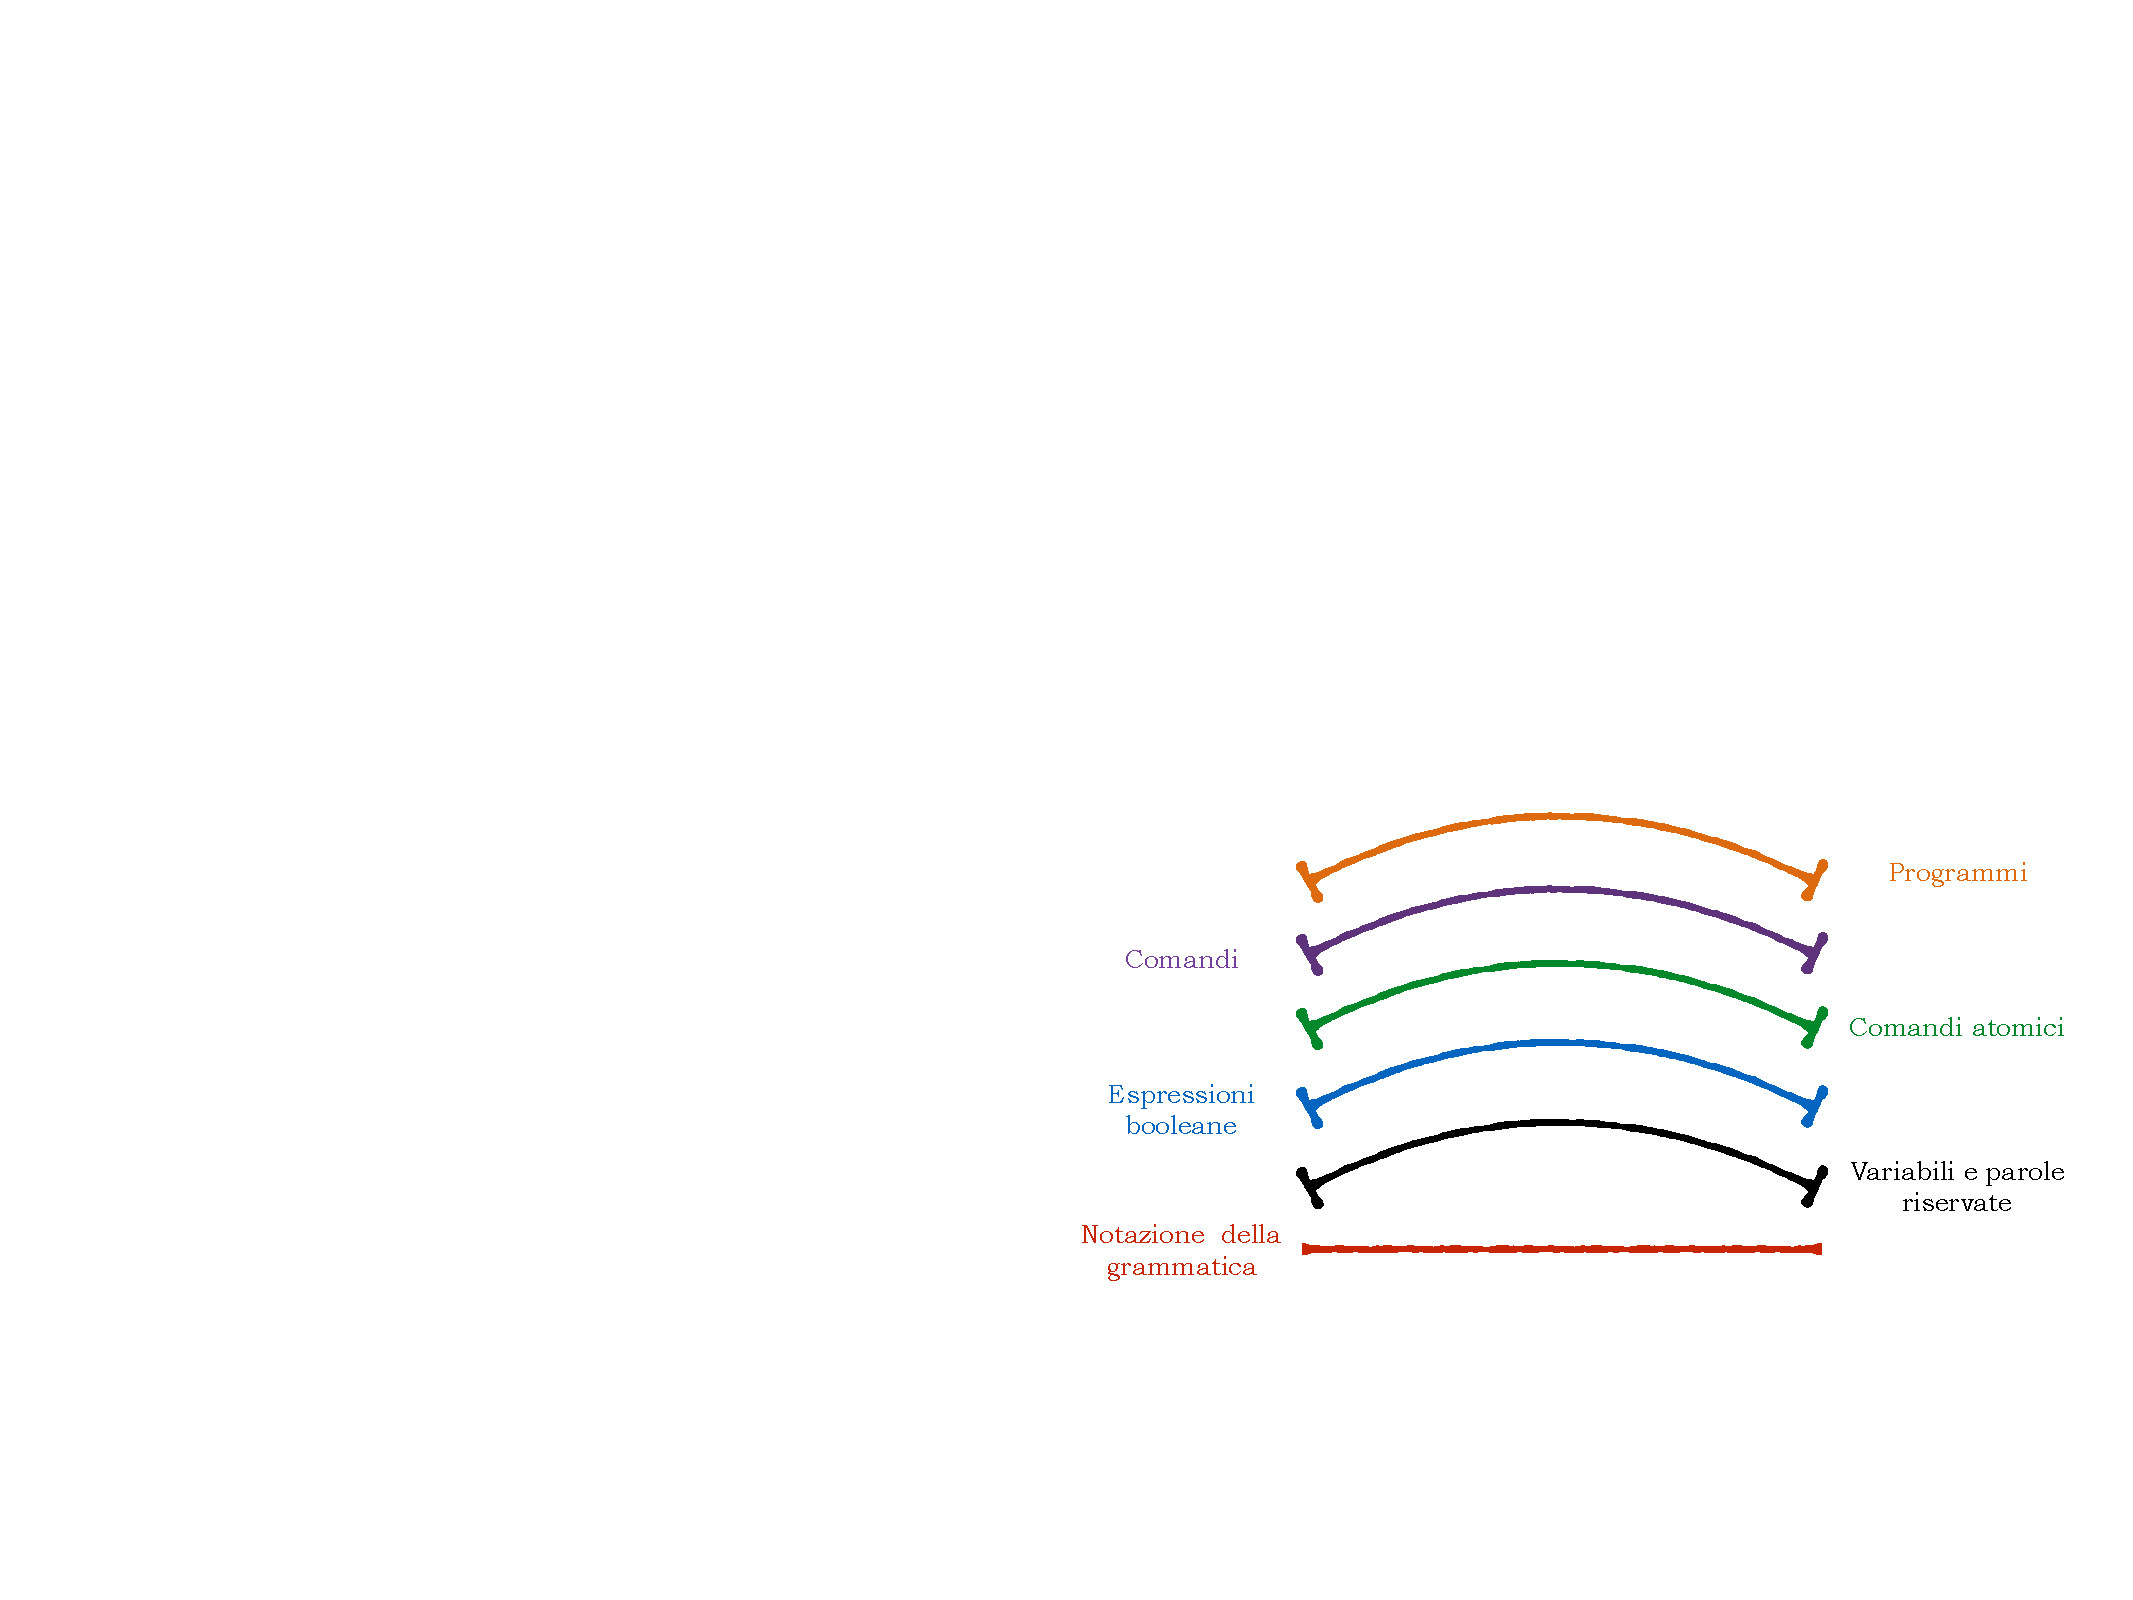
\includegraphics[width=\textwidth]{img/astrazione_linguaggi.pdf}
		\caption{Linguaggio descritto a più livelli di astrazione.}
	\end{figure}

	\noindent
	Un esempio di descrizione a più livelli:
	\begin{equation*}
		\begin{array}{lllll}
			\mathrm{<program>} 		&& S & \Coloneqq & C \\
			\\
			\mathrm{<com>}			&& C & \Coloneqq & A \hspace{1em} | \hspace{1em} C ; C \hspace{1em} | \hspace{1em} \mathrm{if} \: B \: \mathrm{then} \: C \: \mathrm{else} \: C \hspace{1em} | \hspace{1em} \mathrm{while} \: B \: \mathrm{do} \: C \\
			\\
			\mathrm{<atomic \: com>}&& A & \Coloneqq & v \Coloneq B \\
			\\
			\mathrm{<b-expr>}		&& B & \Coloneqq & \mathrm{true} \hspace{1em} | \hspace{1em} \mathrm{false} \hspace{1em} | \hspace{1em} v \hspace{1em} | \hspace{1em} \left(\mathrm{not} \: B\right) \hspace{1em} | \hspace{1em} \left(B \: \mathrm{and} \: B\right) \hspace{1em} | \hspace{1em} \left(B \: \mathrm{or} \: B\right)
		\end{array}
	\end{equation*}\newpage

	\subsection{Analisi semantica}

	Esistono dei vincoli che dipendono dal contesto. Per esempio, l'espressione:
	\begin{equation*}
		I \Coloneq R + 3
	\end{equation*}
	Potrebbe essere sintatticamente corretta ma illegale nel contesto in cui si trova. Infatti, se il linguaggio fosse fortemente \emph{tipato} e prima non ci fosse una dichiarazione di $R$ e di $I$, il comando sarebbe illegale.\newline

	\noindent
	Quindi, stringhe sintatticamente corrette per una certa grammatica sono legali sono in determinati contesti. Questo \textbf{vincolo sintattico} non può essere descritto mediante le grammatiche CF.\newline

	\noindent
	Esistono due \textbf{soluzioni}:
	\begin{itemize}
		\item Utilizzare grammatiche contestuali (CSG). Tuttavia, non esistono algoritmi lineari per il riconoscimento di stringhe generate, quindi non esistono algoritmi efficienti per effettuare il parser delle stringhe di una CSG.
		\item Utilizzare controlli \emph{ad hoc}.
	\end{itemize}
	A causa dei problemi con le grammatiche contestuali, la scelta ricade nell'utilizzare una specifica del linguaggio mediante una grammatica CF (\textbf{sintassi}) e successivamente, come parte della semantica (\textcolor{Red3}{\textbf{semantica statica}}) specificare i vincoli contestuali.\newpage

	\subsection{Semantica dinamica}

	La \textbf{semantica} ricerca esattezza e flessibilità:
	\begin{itemize}
		\item \textbf{Esattezza}: descrizione precisa e non ambigua di ogni costrutto sintatticamente corretto, per sapere cosa accadrà durante l'esecuzione
		\item \textbf{Flessibilità}: nessuna anticipazione delle scelte che devono essere demandate dall'implementazione.
	\end{itemize}
	La \textcolor{Red3}{\textbf{semantica dinamica}} risponde ad alcune problematiche, come il significato di alcuni comandi, che cosa fanno i costrutti, generatori di compilatori. Il suo \textbf{utilizzo è fondamentale poiché specifica gli effetti della sintassi sulla rappresentazione astratta della macchina}, quest'ultima chiamata \textbf{stato}.\newline
	Quindi, per ogni costrutto, va descritto il significato della sua esecuzione come trasformazione di stato. Infatti, l'astrazione della macchina nel concetto di stato consente di dare al costrutto un significato puro, indipendente dalla macchina, quindi senza restrizioni.\newline

	\noindent
	\begin{boxdef}
		La \textcolor{Red3}{\textbf{semantica}} \textbf{attribuisce un significato ad ogni frase sintatticamente corretta}.
	\end{boxdef}
	\begin{boxdef}
		Con \textcolor{Red3}{\textbf{significato}} \textbf{si intendono le entità autonome che esistono indipendentemente dai segni che vengono utilizzati per descriverle}.
	\end{boxdef}

	\noindent
	Esiste un \textbf{legame forte tra sintassi e semantica}:
	\begin{itemize}
		\item La \textbf{sintassi} è utilizzato come metodo finito per rappresentare un insieme infinito di programmi, la cui sola cosa analizzabile è la struttura;
		\item La \textbf{semantica} è utilizzata come metodo finito, infatti segue la struttura della sintassi, per dare significato a tutti gli elementi dell'insieme infinito dei programmi.
	\end{itemize}\newpage

	\subsection{Induzione matematica e strutturale}

	La semantica segue la struttura della sintassi, mentre quest'ultima è definita descrivendo gli elementi base e componendo questi elementi, attraverso regole, in elementi composti.\newline
	
	\begin{boxdef}
		Questa forma di definizione si chiama \textcolor{Red3}{\textbf{induzione}} e più formalmente è: data un insieme $A$ ed una relazione binaria $< \subseteq A \times A$ ben fondata (senza catene discendenti infinite), se $A = Nat$ si ha \textbf{induzione matematica}; se $A = L\left(G\right)$ è un linguaggio generato da una grammatica $G$, allora si ha \textbf{induzione strutturale}.
	\end{boxdef}\:\newline

	\noindent
	\begin{boxdef}
		Il \textcolor{Red3}{\textbf{principio di induzione strutturale}} si basa sulla seguente definizione. Per dimostrare che una proprietà è valida per tutti gli elementi di una categoria sintattica:
		\begin{enumerate}
			\item \textbf{Base induttiva}: si dimostra la proprietà per tutti gli elementi base della categoria, quelli che non hanno nessun elemento come componente;
			\item \textbf{Passo induttivo}: si dimostra la proprietà per tutti gli elementi composti assumendo che la proprietà sia verificata da tutti i loro componenti immediati.
		\end{enumerate}
	\end{boxdef}\newpage

	\noindent
	Ecco una dimostrazione d'\textcolor{Green4}{\textbf{esempio}} di induzione.
	\begin{proof}[\textbf{Dimostrazione induttiva}]
		Dimostrare che:
		\begin{equation*}
			\sum_{i = 1}^{n} i = \dfrac{n \left( n + 1 \right)}{2} \hspace{2em} \text{con } n \ge 1
		\end{equation*}
		La \textbf{base induttiva} è con $n$ pari ad $1$, quindi sostituendo:
		\begin{equation*}
			n = 1 \hspace{2em} \sum_{i = 1}^{1} i = 1 = \dfrac{1 \left( 1 + 1 \right)}{2}
		\end{equation*}
		Per il \textbf{passo induttivo} si suppone che sia vero per $n$ considerando dunque come passo induttivo l'equazione iniziale. Si dimostra per $n + 1$:
		\begin{equation*}
			\begin{array}{rll}
				\displaystyle\sum_{i=1}^{n+1} i & = & \dfrac{ \left(n+1\right) \left(n+2\right) }{2} \\
				\\
				\displaystyle\sum_{i=1}^{n+1} i \triangleq \underbrace{\sum_{i=1}^{n} i + \left(n+1\right)}_{\text{per definizione}} & = & \underbrace{\dfrac{n \left(n+1\right)}{2}}_{\text{ip. induttiva}} + \: n + 1 \\
				\\
				& = & \dfrac{n \left(n+1\right) + 2n + 2}{2} = \dfrac{n^{2} + n + 2n + 2}{2} \\
				\\
				& = & \dfrac{\left(n+1\right) n + \left(n+1\right) 2}{2} = \dfrac{\left(n+1\right) \left(n+2\right)}{2}
			\end{array}
		\end{equation*}
	\end{proof}\newpage

	\subsection{Un significato, tante rappresentazioni}
	
	Durante l'implementazione di un algoritmo, ci sono alcuni aspetti che un programmatore deve tenere in considerazione:
	\begin{itemize}
		\item Il \textbf{comportamento dell'I/O} è un aspetto che interessa l'\textbf{implementatore}, ovvero colui che descrive funzionalità attraverso le trasformazioni di stato della macchina.
	
		\item La funzione descritta dall'algoritmo è un aspetto che interessa il \textbf{progettista}, ovvero colui che progetta costrutti del linguaggio per consentire l'implementazione di certe funzionalità.
	
		\item Le \textbf{proprietà e invarianti} sono di interesse dello sviluppatore, ovvero colui che è focalizzato sull'utilizzo e sulla combinazione dei costrutti così di preservare invarianti o da garantire proprietà desiderate.
	\end{itemize}
	Di fatto tutte queste rappresentazioni, e i loro punti di vista, sono equivalenti, guardano solo il problema da diversi punti. Per questo motivo, nascono \textbf{diversi tipi di semantica}:
	\begin{itemize}
		\item \textbf{Semantica denotazionale}: descrive funzionalità. Studia gli effetti dell'esecuzione e cerca proprietà del programma studiando proprietà della funzione calcolata;
		
		\item \textbf{Semantica assiomatica}: descrive proprietà. Necessaria per fare deduzioni logiche, a partire da assiomi dati, su parti del programma (dimostrazioni di correttezza);
		
		\item \textbf{Semantica operazionale}: descrive trasformazioni di stato. Opera con l'obbiettivo di analizzare il processo per arrivare ad un risultato finale. In parole povere, ha l'obbiettivo di analizzare come i risultati finali vengono prodotti (implementazione di un interprete).
	\end{itemize}\newpage

	\subsubsection{Semantica denotazionale}
	
	\begin{boxdef}
		La \textcolor{Red3}{\textbf{semantica denotazionale}} è un modello matematico dei programmi basato sulla ricorsione. È la semantica più \dquotes{astratta} con cui descrivere i programmi.
	\end{boxdef}
	
	\noindent
	Il \textbf{processo di costruzione} della semantica denotazionale \textbf{per un linguaggio} si articola in due passaggi fondamentali:
	\begin{enumerate}
		\item Definizione di un oggetto matematico per ogni entità del linguaggio;
		
		\item Definizione di una funzione che esegue un \emph{mapping} delle istanze delle entità del linguaggio in istanze dei corrispondenti oggetti matematici.
	\end{enumerate}
	Il modello matematico utilizzato è quello delle funzioni matematiche ricorsive, ovvero un programma corrispondente ad una funzione tra stati della macchina:
	\begin{equation*}
		E: \mathrm{Prog} \longrightarrow \left( \left(\mathrm{Var} \rightarrow \mathrm{Val}\right) \longrightarrow \left(\mathrm{Var} \rightarrow \mathrm{Val}\right) \right)
	\end{equation*}
	L'equivalenza di programma si dimostra mediante equivalenza tra funzioni matematiche.\newline
	
	\noindent
	Dunque la \textbf{semantica denotazionale è un oggetto puramente matematico} che descrive gli effetti semplicemente manipolando oggetti matematici.\newline
	In particolare, vengono \textbf{analizzati gli effetti dell'esecuzione del programma}, descrivendo l'effetto dell'esecuzione di una sequenza di comandi separati da \dquotes{;} attraverso la composizione degli effetti dei singoli comandi da sinistra verso destra.\newline
	Con \textbf{effetto di ogni comando} si intende la funzione che dato uno stato produce un nuovo stato.\newline
	
	\noindent
	Il suo utilizzo è \textcolor{Green4}{\textbf{utile}} per:
	\begin{itemize}
		\item Dimostrare la correttezza dei programmi;
		\item Ragionare formalmente sui programmi;
		\item Aiutare la progettazione dei linguaggi;
		\item Generare i compilatori.s
	\end{itemize}
	Purtroppo, a causa della sua elevata complessità, risulta \textcolor{Red3}{\textbf{poco utile}} per gli utilizzatori dei linguaggi.\newpage
	
	\noindent
	Per \textcolor{Green4}{\textbf{esempio}}, si definisce la funzione di valutazione $E\exec{P}\sigma$ che valuta il programma $P$ sulla memoria $\sigma$, restituendo in output $\sigma'$ che corrisponde alla memoria $\sigma$ modificata dal programma $P$.\newline
	
	\noindent
	Il programma $P$ è formato nel seguente modo:
\begin{lstlisting}[language=C]
P:
	z := 2;
	y := z;
	y := y+1;
	z := y;\end{lstlisting}
	La semantica denotazionale consente questa rappresentazione:
	\begin{equation*}
		\begin{array}{lll}
			E\exec{P}\left(z = \bot, y = \bot\right) & = & \left(E\exec{ z \coloneq y } \circ E\exec{ y \coloneq y+1 } \circ E\exec{ y \coloneq z } \circ E\exec{ z \coloneq 2 }\right) \left[z = \bot, y = \bot\right] \\
			\\
			&=& \left(E\exec{ z \coloneq y } \left( E\exec{ y \coloneq y+1 } \left( E\exec{ y \coloneq z } \left( E\exec{ z \coloneq 2 } \right) \left[z = \bot, y = \bot\right]\right)\right)\right) \\
			\\
			&=& \left(E\exec{ z \coloneq y } \left( E\exec{ y \coloneq y+1 } \left( E\exec{ y \coloneq z } \left[z = 2, y = \bot\right]\right)\right)\right) \\
			\\
			&=& \left(E\exec{ z \coloneq y } \left( E\exec{ y \coloneq y+1 } \left[z = 2, y = 2\right]\right)\right) \\
			\\
			&=& \left(E\exec{ z \coloneq y } \left[z = 2, y = 3\right]\right) \\
			\\
			&=& \left[z = 3, y = 3\right]
		\end{array}
	\end{equation*}
	Ad ogni passo viene consumata una valutazione, la quale modifica in memoria i valori tra parentesi quadre.\newpage
	
	\subsubsection{Semantica assiomatica}
	
	\begin{boxdef}
		La \textcolor{Red3}{\textbf{semantica assiomatica}} è un modello matematico dei programmi basato sulla logica formale, ovvero il calcolo dei predicati.
	\end{boxdef}
	
	\noindent
	L'\textbf{obbiettivo} della semantica assiomatica è la verifica formale di programmi. Per farle, vengono utilizzati assiomi e regole di inferenza. Le \textbf{espressioni logiche} utilizzate sono chiamate \textbf{asserzioni}:
	\begin{itemize}
		\item \textbf{Precondizione}: asserzione prima di un comando che dichiara le relazioni e i vincoli validi prima dell'esecuzione del comando;
		
		\item \textbf{Postcondizione}: asserzione che segue il comando che descrive cosa vale dopo l'esecuzione;
		
		\item \textbf{\emph{Weakest precondition}}: una precondizione meno restrittiva che garantisce la post-condizione.
	\end{itemize}
	Quindi, la semantica assiomatica consente di \textbf{dimostrare proprietà parziali di correttezza}: quando lo stato iniziale rispetta la precondizione e il programma termina, allora lo stato finale soddisfa la postcondizione.\newline
	
	\noindent
	Dato che la semantica assiomatica è un sistema logico, deve \textbf{godere di due proprietà}:
	\begin{itemize}
		\item \textbf{Correttezza} (\emph{soundness}), ogni proprietà derivabile nel sistema vale per il programma;
		
		\item \textbf{Completezza}, ogni proprietà che vale per il programma è derivabile nel sistema di regole.
	\end{itemize}\newpage

	\noindent
	Per \textcolor{Green4}{\textbf{esempio}}, si definisce la notazione $\left\{P\right\}$ \emph{statement} $\left\{Q\right\}$. Questa semantica si calcola mediante un sistema di prova: si ha una tripla da verificare e si cerca di dimostrarla applicando le regole.\newline
	
	\noindent
	Il programma $P$ è formato nel seguente modo:
	\begin{lstlisting}[language=C]
		P:
		z := 2;
		y := z;
		y := y+1;
		z := y;\end{lstlisting}
	\begin{figure}[!htp]
		\centering
		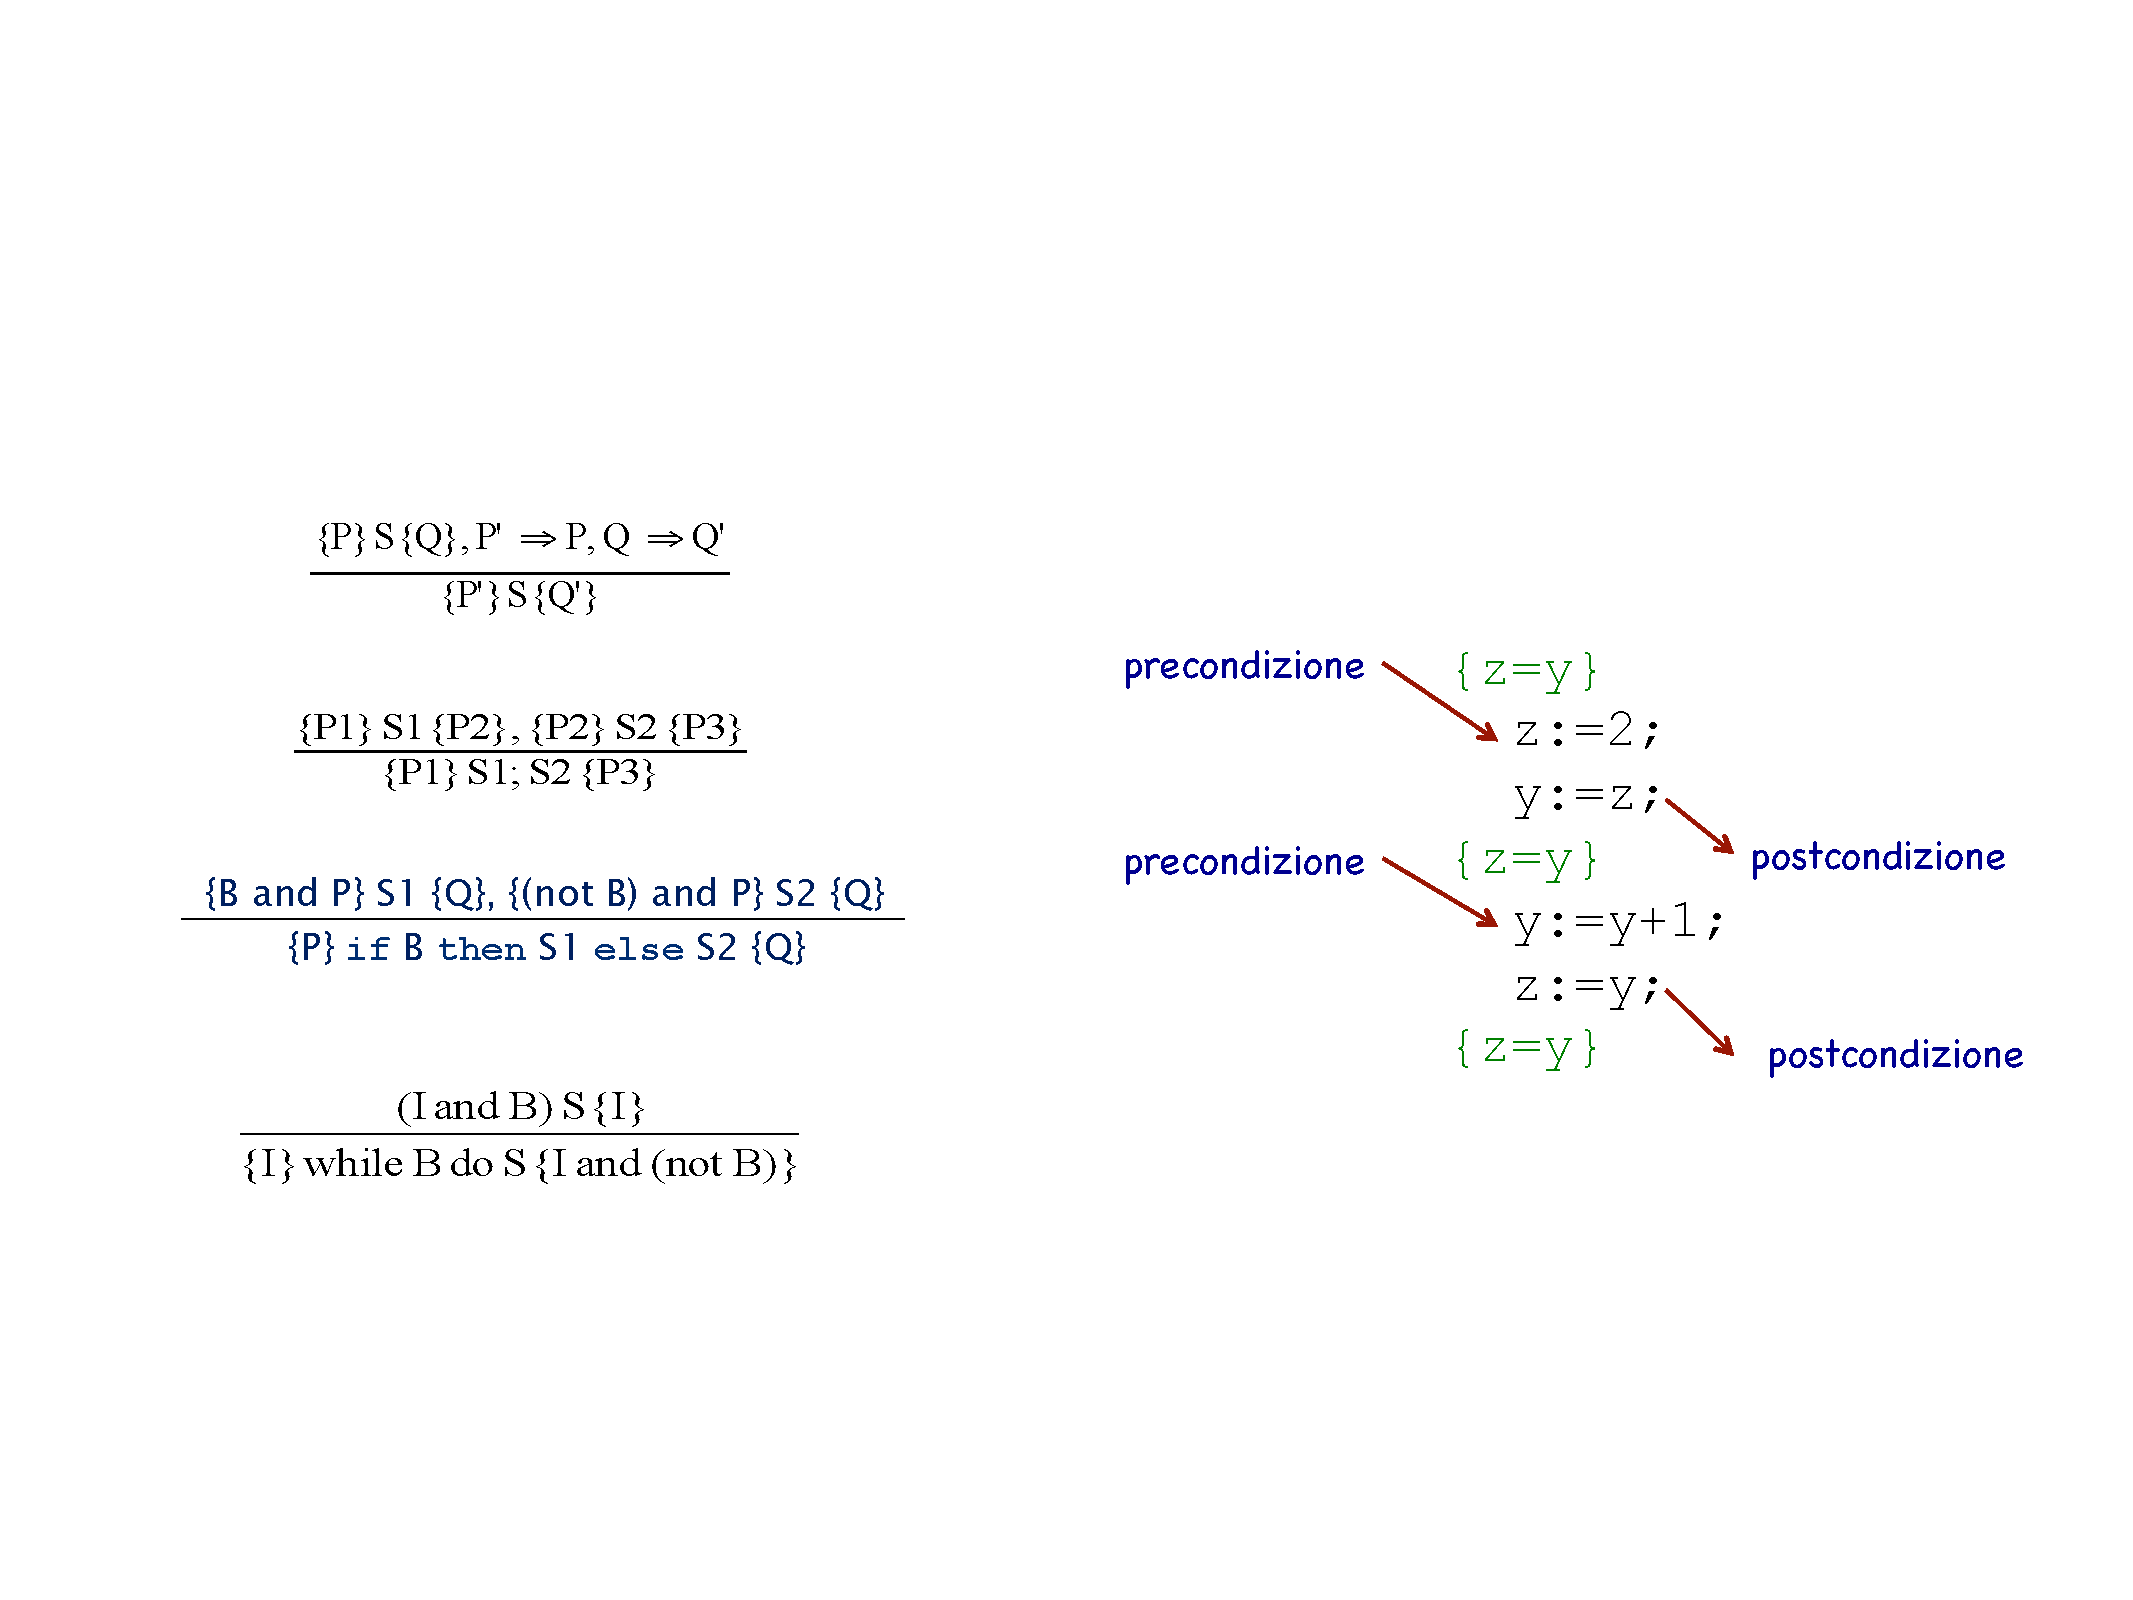
\includegraphics[width=\textwidth]{img/eg-semantica_assiomatica.pdf}
	\end{figure}\newpage

	\subsubsection{Semantica operazionale}
	
	\begin{boxdef}
		La \textcolor{Red3}{\textbf{semantica operazionale}} è un modello matematico dei programmi basato sui sistemi di transizione.
	\end{boxdef}
	
	\noindent
	La semantica operazionale descrive il significato del programma \textbf{eseguendo i suoi comandi su una macchina}, simulata o reale. La \textbf{trasformazione dello stato definisce il significato del comando}. Quindi, lo stato è la rappresentazione astratta della macchina.
	
	Inoltre, la semantica operazionale è necessaria per definire una macchina astratta.\newline
	
	\noindent
	Il modello matematico utilizzato è quello dei sistemi di transizione. Per \textcolor{Green4}{\textbf{esempio}}, si consideri la funzione memoria $\sigma: \mathrm{Var} \rightarrow \mathrm{Val}$ che associa valori alle variabili. Con \textbf{stato} si identifica una coppia nel programma ancora da eseguire:
	\begin{equation*}
		\mathrm{Stato} = \left\langle P,\sigma \right\rangle
	\end{equation*}
	Ad ogni passo, viene eseguita un'operazione e la configurazione o stato cambia. La chiusura transitiva descrive l'esecuzione completa.\newline
	Inoltre, questa semantica esegue i comandi separai da \dquotes{;} sequenzialmente e nell'ordine in cui compaiono da sinistra a destra.
	
	Infine, nonostante sia una delle forme più concrete di semantica, viene eseguita comunque un'astrazione di come il programma viene eseguito, quindi essa è indipendente dall'architettura.\newline
	
	\noindent
	Per \textcolor{Green4}{\textbf{esempio}}, il programma $P$ è formato nel seguente modo:
	\begin{lstlisting}[language=C]
		P:
		z := 2;
		y := z;
		y := y+1;
		z := y;\end{lstlisting}
	\begin{gather*}
		\left\langle z \coloneq 2; \hspace{1em} y \coloneq z; \hspace{1em} y \coloneq y+1; \hspace{1em} z \coloneq y, \left[z=\bot,y=\bot\right]\right\rangle \\
		\left\langle y \coloneq z; \hspace{1em} y \coloneq y+1; \hspace{1em} z \coloneq y, \left[z=2,y=\bot\right]\right\rangle \\		
		\left\langle y \coloneq y+1; \hspace{1em} z \coloneq y, \left[z=2,y=2\right]\right\rangle \\
		\left\langle z \coloneq y, \left[z=2,y=3\right]\right\rangle \\
		\left\langle \varepsilon, \left[z=3,y=3\right]\right\rangle
	\end{gather*}\newpage
	
	\subsubsection{Composizionalità}
	
	\begin{boxdef}
		La \textcolor{Red3}{\textbf{composizionalità}} è la proprietà per cui il significato di ogni programma deve essere in funzione del significato dei costituenti immediati.
	\end{boxdef}
	
	\noindent
	La composizionalità è una \textbf{proprietà della semantica} necessaria per caratterizzare i comportamenti e significati di sistemi che possono avere infiniti elementi.\newline
	
	\noindent
	L'\textbf{importanza} della composizionalità è dovuta alla necessità di analizzare le proprietà di un programma. Infatti, per farlo è necessario capire che cosa fa e dunque capire la semantica in ogni sua forma. L'analisi diventa molto più semplice grazie alla \textbf{modularità}, la quale è \textbf{garantita dalla composizionalità}. Quindi, anche nei software di grandi dimensioni, è possibile analizzare il codice separatamente nei suoi moduli, per poi ricomporre il risultato dell'analisi componendo i risultati ottenuti sui singoli moduli.
	
	\longline
	
	\subsubsection{Equivalenza}
	
	\begin{boxdef}
		L'\textcolor{Red3}{\textbf{equivalenza}} è vera quando due programmi hanno la stessa semantica.
	\end{boxdef}
	
	\noindent
	Per capire se due programmi sono equivalenti, viene osservata la relazione tra input e output. Se la relazione è la stessa, indipendentemente da come l'algoritmo la calcola, allora sono equivalenti. Quindi, solo caratterizzando la funzionalità I/O è possibile determinare questa caratteristica.\newline
	
	\noindent
	Infine, l'equivalenza è necessaria in varie fasi di analisi:
	\begin{itemize}
		\item \textbf{Correttezza}, per dimostrare che il programma scritto calcola esattamente la funzione attesa;
		
		\item \textbf{Equivalenza di programmi}, per dimostrare che due programmi calcolano la stessa funzione;
		
		\item \textbf{Efficienza}, Dati due programmi che calcolano la stessa funzione, si vuole dimostrare quale lo fa in modo più efficiente.
	\end{itemize}\newpage
	
	\subsection{Sintassi}
	
	\subsubsection{Stato (ambiente e memoria)}
	
	Per descrivere il significato dei programmi, è necessario introdurre due entità fondamentali: ambiente e memoria.\newline
	
	\noindent
	\begin{boxdef}
		L'\textcolor{Red3}{\textbf{ambiente}} (\textbf{\emph{environment}}) \textbf{è un insieme di legami (\emph{bindings}) tra identificatori e denotazioni}.
	\end{boxdef}
	Inoltre, l'ambiente specifica quali nomi sono usati e per quali oggetti, solitamente possono essere legati ad un tipo, ad un valore, ad una locazione. Quindi, i \emph{binding}\footnote{In breve sarebbero le API (\emph{Application Programming Interface}): \href{https://en.wikipedia.org/wiki/Language_binding}{link fonte}.} sono associati ai nomi, i quali possono essere variabili, costanti, procedure, e altro. I nomi sono solo un'entità separata dall'oggetto che denotano, infatti esso potrebbe essere usato in contesti diversi per rappresentare valori differenti.\newline
	
	\noindent
	\begin{boxdef}
		La \textcolor{Red3}{\textbf{memoria}} (\textbf{\emph{store}}) \textbf{è un insieme di effetti sugli identificatori (causati da assegnamenti)}.
	\end{boxdef}
	Essa è una mappa che solitamente rappresenta la storia, cioè l'evoluzione, delle variazioni dei valori associati agli identificatori. In altre parole, fornisce un \emph{binding} tra locazione e valore.\newline
	Si ricorda, che la memoria è fortemente legato all'approccio imperativo, infatti i linguaggi funzionali pure non ne hanno bisogno dato che non gestiscono variabili che cambiano durante l'esecuzione del programma.
	
	\longline
	
	\subsubsection{Categorie sintattiche}
	
	\begin{boxdef}
		Le \textcolor{Red3}{\textbf{categorie sintattiche}} \textbf{sono la classificazione dei costrutti in funzione del loro significato atteso, ovvero della classe di effetti che ha la loro esecuzione causa.}
	\end{boxdef}
	Quindi, esse sono classi che rappresentano un diverso tipo di significato, effetto, esecuzione di un programma.\newline
	
	\noindent
	Le categorie sintattiche si distinguono in: \textbf{espressioni}, \textbf{comandi} e \textbf{dichiarazioni}. Formalmente, le categorie sono i simboli non terminali della grammatica classificati in funzione di cosa modificano dello stato e come lo modificano.\newpage
	
	\subsubsection{Espressioni}
	
	Le \textcolor{Red3}{\textbf{espressioni}} \textbf{nascono dalla necessità di avere una categoria sintattica che consenta di rappresentare e denotare i valori}. Esse possono essere espresse con dei vincoli, per esempio il tipo.\newline
	
	\noindent
	Nonostante le espressioni denotino i valori, esse \textbf{non sono locazioni di memoria}. Quest'ultime sono legati all'architettura (struttura) di una macchina, mentre le espressioni fanno riferimento allo specifico linguaggio di programmazione.\newline
	
	\noindent
	\begin{boxdef}
		Due espressioni sono considerate \textcolor{Red3}{\textbf{equivalenti}} \textbf{se vengono valutate nello stesso valore in tutti gli stati di computazione. Anche eventuali \emph{side-effect} devono essere gli stessi}.
	\end{boxdef}
	
	Infatti, due espressioni possono essere diverse ma essere valutate nello stesso valore. Per \textcolor{Green4}{\textbf{esempio}}, l'espressione logica \textsf{not(a and b)} è logicamente (semanticamente) equivalente ad \textsf{(not a) or (not b)} ma sono sintatticamente diverse.
	
	\longline
	
	\subsubsection{Dichiarazioni}
	
	Le \textcolor{Red3}{\textbf{dichiarazioni}} \textbf{sono la categoria sintattica che consente la creazione o la modifica dei legami associati agli identificatori, ovvero gli ambienti}.\newline
	
	\noindent
	Esse nascono con l'obbiettivo di utilizzare i valori. Per farlo, è stato necessario creare, utilizzare e modificare \textbf{legami} tra nomi e valori.\newline
	
	\noindent
	Inoltre, gli le modifiche agli ambienti sono trasformazioni \textbf{reversibili}, ovvero che le trasformazioni hanno valenza esclusivamente all'interno del raggio d'azione (\emph{scope}) attuale dell'identificatore. In altre parole, i linguaggi di programmazione delimitano la validità di un ambiente. Più precisamente con \textbf{reversibili si intende} che una volta terminata la validità di un ambiente, le modifiche verranno annullate.\newline
	
	\noindent
	\begin{boxdef}
		Due dichiarazioni sono \textcolor{Red3}{\textbf{equivalenti}} \textbf{se producono lo stesso ambiente e la stessa memoria in caso di \emph{side-effect} in tutti gli stati di computazione}.
	\end{boxdef}
	A causa del \emph{side-effect} è necessario che l'equivalenza richieda che due dichiarazioni generino le stesse identiche modifiche a tutto lo stato di computazione.\newpage
	
	\subsubsection{Comandi}
	
	I \textcolor{Red3}{\textbf{comandi}} \textbf{sono richieste di modifica dello stato di computazione, ed in particolare della memoria}.\newline
	
	\noindent
	Le trasformazioni sono \textbf{irreversibili}, ovvero sono definite nell'esecuzione del programma. Quindi, per annullarle è necessario eseguire altri comandi e altre trasformazioni che consentono di tornare alla stessa memoria iniziale. Quindi, i comandi non sono altro che funzioni di trasformazione e devono essere \textbf{eseguiti} per poter attuare la corrispondente trasformazione (irreversibile) della memoria.
	
	\begin{boxdef}
		Due comandi sono \textcolor{Red3}{\textbf{equivalenti}} \textbf{se per ogni stato (memoria) in input producono lo stesso stato (memoria) in output}.
	\end{boxdef}

	\longline

	\subsection{Semantica operazionale: sistemi di transizione}
	
	I \textcolor{Red3}{\textbf{sistemi di transizione}} \textbf{sono strumenti astratti mirati a specificare senza ambiguità e senza dipendenza dalla macchina, cosa fa un linguaggio}. Le sue caratteristiche principali sono:
	\begin{itemize}
		\item Matematicamente precisi;

		\item Molto concisi;

		\item Metodo di specifica generale che consente l'astrazione;

		\item Specificano cosa viene calcolato per induzione sulla struttura sintattica del linguaggio.
	\end{itemize}
	Inoltre, sfruttando la definizione induttiva del linguaggio, consentono di definire il significato mediante induzione sull'\emph{abstract syntax tree}. Quindi, viene \textbf{usata l'induzione strutturale matematica per ragion sui programmi}.\newline
	
	\noindent
	\begin{boxdef}
		Formalmente: \textbf{un \textcolor{Red3}{sistema di transizione} è una struttura $\left(\Gamma, \rightarrow\right)$, dove $\Gamma$ è un insieme di elementi $\gamma$ chiamati configurazioni e la relazione binaria $\rightarrow \subseteq \Gamma \times \Gamma$ è chiamata relazione di transizione. Se $\Gamma_{T} \subseteq \Gamma$ è un insieme di configurazioni terminali, il sistema è detto terminale.}
	\end{boxdef}\newpage
	
	\subsection{Esempio di un linguaggio reale ($PL_{0}$)}\label{esempio di un linguaggio reale PL0}
	
	Un esempio di linguaggio reale è $PL_{0}$ strutturato nel seguente modo:
	\begin{figure}[!htp]
		\centering
		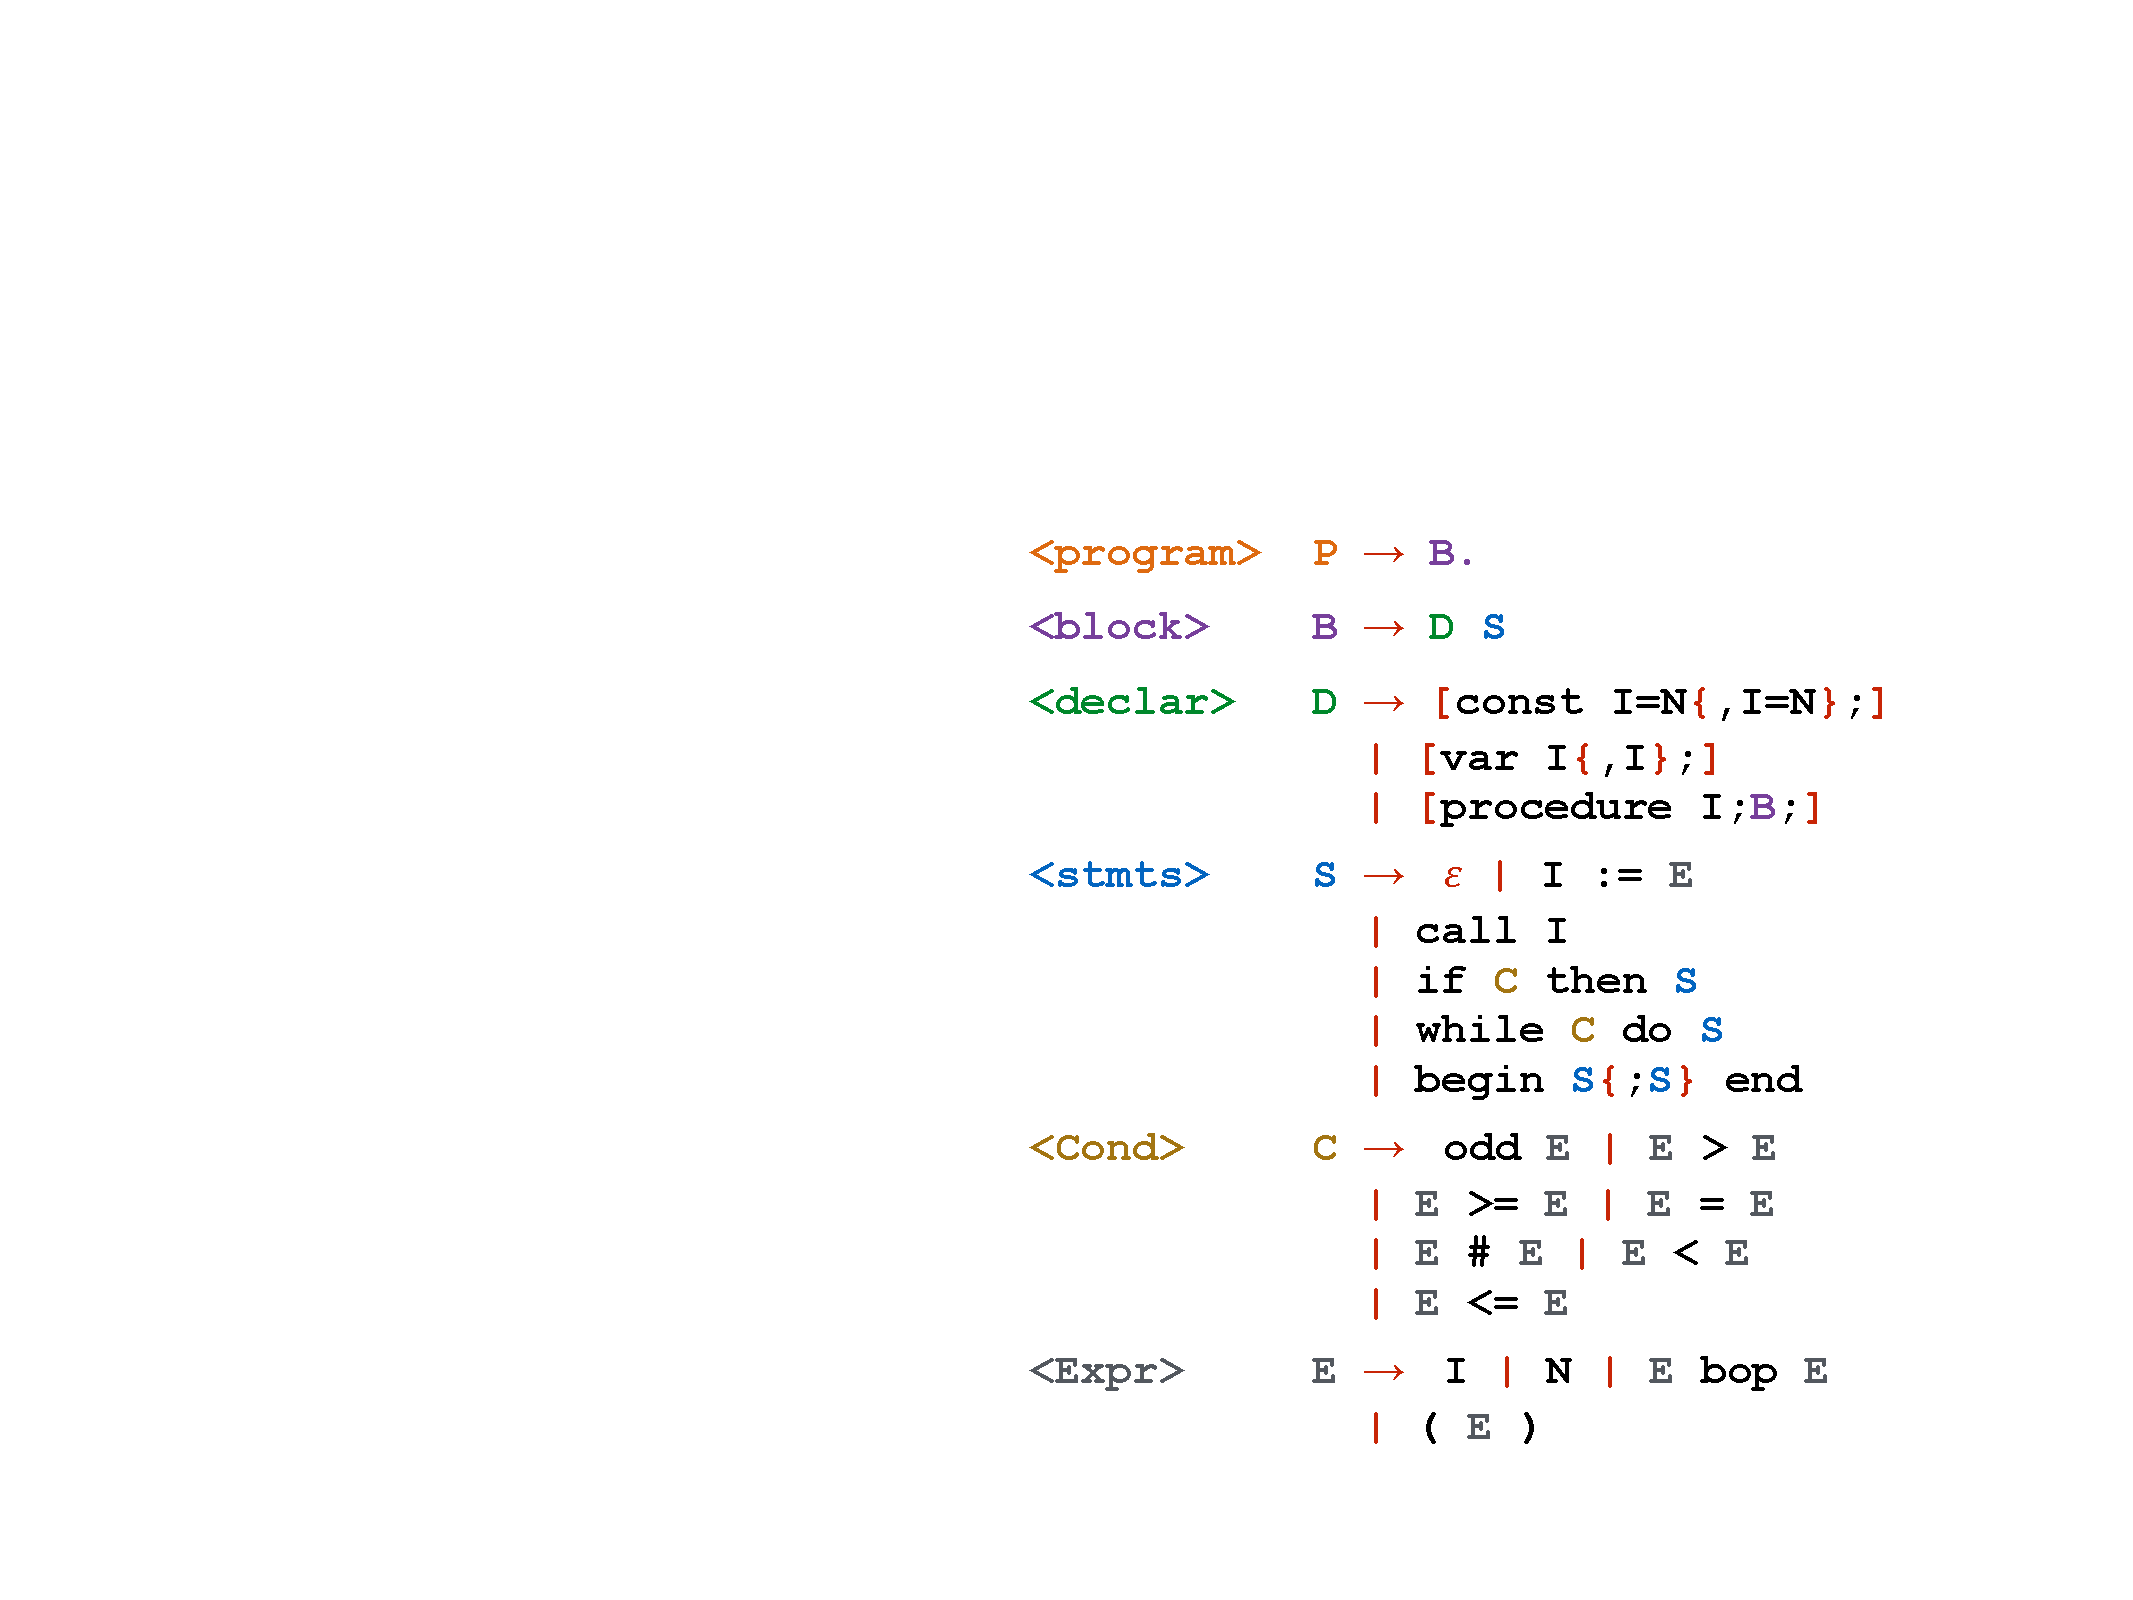
\includegraphics[width=.6\textwidth]{img/pl0.pdf}
	\end{figure}
	
	\begin{itemize}
		\item I programmi $P$ sono blocchi.
		
		\item I blocchi $B$ sono una dichiarazione $D$ seguita da un comando $S$, entrambi liberi dal contesto.
		
		\item Le dichiarazioni $D$ sono dichiarazioni di valori costanti con nome (const), dichiarazioni di variabili (var) e dichiarazioni di procedure.
		
		\item I nomi sono gli identificatori $I$, considerati parte del vocabolario, e $N$ sono i numeri naturali, anch'essi considerati parte del vocabolario.
		
		\item Non esiste il concetto di tipo poiché l'unico dato ammesso è intero.
		
		\item I comandi sono:
		\begin{itemize}
			\item Comando vuoto;
			\item Assegnamento di un valore ad un identificatore;
			\item Chiamata ad una procedura mediante il suo nome;
			\item Comando condizionale che esegue un comando al verificarsi di una condizione booleana;
			\item Ciclo che ripete un comando finché una data condizione è vera;
			\item Composizione sequenziale di comandi.
		\end{itemize}
	
		\item Le condizioni $C$ sono espressioni che hanno al loro interno valori booleani.
		
		\item Le espressioni $E$ sono identificatori, valori naturali, operazioni tra espressioni e espressioni tra parentesi.
	\end{itemize}\newpage

	\section{Espressioni}
	
	\subsection{Introduzioni}
	
	Per manipolare i valori è necessario rappresentarli e per questo motivo vengono utilizzate le espressioni. Quest'ultime, devono essere valutate per dare un valore e con valore non viene intesa la locazione di memoria: i valori fanno parte dello specifico linguaggio di programmazione, mentre la locazione è parte della struttura dell'architettura. Quindi, la locazione di memoria modella il modo in cui il linguaggio di programmazione si relazione alla macchina sottostante.
	
	\longline
	
	\subsection{Descrivere le espressioni}
	
	Per associare significati e valori alle \textbf{espressioni}, esse \textbf{devono essere valutate}.\newline
	
	\noindent
	Il \textbf{valore ottenuto mediante la valutazione} è chiamato \textbf{valore esprimibile}, poiché è un \textbf{valore che può essere espresso attraverso la sintassi del linguaggio di programmazione}, e in particolare attraverso la sintassi delle espressioni.\newline
	
	\noindent
	\textbf{Formalmente} con \textcolor{Red3}{\textbf{valore esprimibile}} si intende l'unione tra i tipi booleani e interi:
	\begin{equation*}
		Eval = bool \cup int \hspace{2em} \text{con metavariabile } ev
	\end{equation*}
	Per metavariabile si intende qualsiasi valore esprimibile.\newline
	
	\noindent
	Per \textcolor{Green4}{\textbf{esempio}}, un linguaggio come $PL_{0}$ (paragrafo \ref{esempio di un linguaggio reale PL0}), si hanno espressioni che rappresentano interi e identificatori, e indirettamente anche booleani in quanto le condizioni corrispondono a valori booleani (e.g. $3=3$ è \emph{true}, mentre $3\#3$ è \emph{false}).\newline
	
	\noindent
	Dal punto di vista \textbf{sintattico}, i \textbf{costituenti elementari delle espressioni} sono \textbf{letterali} (costanti e identificatori), i quali sono \textbf{composti mediante operatori}.\newline
	
	\noindent
	\textbf{Per concludere}, un'espressione è un oggetto sintattico composto da operatori, operandi (che sono espressioni alla fine), parentesi e funzioni/procedure.\newpage
	
	\subsection{Caratteristiche}
	
	Ecco qua di seguito gli \textbf{aspetti che caratterizzano le espressioni}:
	\begin{itemize}
		\item \textcolor{Red3}{\textbf{Notazione}} che specifica in che modo gli operandi e gli operatori vengono rappresentati. Inoltre, indica su quali operandi un operatore opera.
		\begin{itemize}
			\item Paragrafo \ref{notazione} sulla notazione
			\item Paragrafo \ref{notazione post-fissa} sulla notazione post-fissa
			\item Paragrafo \ref{notazione pre-fissa} sulla notazione pre-fissa
			\item Paragrafo \ref{notazione in-fissa} sulla notazione in-fissa
		\end{itemize}
		
		\item \textcolor{Red3}{\textbf{Regole di precedenza}} tra operatori
		
		\item \textcolor{Red3}{\textbf{Regole di associatività}} degli operatori
		
		\item \textcolor{Red3}{\textbf{Ordine di valutazione degli operandi}}
		
		\item \textcolor{Red3}{\textbf{Presenza di \emph{side-effects}}}, ovvero qualunque effetto che non consiste puramente nella rappresentazione di valori;
		
		\item \textcolor{Red3}{\textbf{\emph{Overloading} degli operatori}}, ovvero simboli di operatori che hanno significati diversi a seconda del tipo degli operatori a cui sono applicati.
		
		\item \textcolor{Red3}{\textbf{Espressioni con tipi misti}}
	\end{itemize}
	
	\longline
	
	\subsubsection{Notazione}\label{notazione}
	
	A seconda di \textbf{come viene rappresentata l'espressione}, \textbf{varia anche il modo in cui viene determinata la semantica} e di conseguenza varia la sua valutazione.\newline
	
	\noindent
	Esistono \textbf{diversi modi per denotare le espressioni}:
	\begin{itemize}
		\item Notazione \textbf{in-fissa}, per esempio $a+b$
		\item Notazione \textbf{pre-fissa} (polacca), per esempio $+ab$
		\item Notazione \textbf{post-fissa} (polacca inversa), per esempio $ab+$
	\end{itemize}
	La notazione in-fissa è quella più utilizza nelle espressioni aritmetiche poiché più intuitiva, ma sono necessarie altre regole per eliminare l'ambiguità. Nelle altre notazioni (pre e post fissa), l'\textcolor{Red3}{\textbf{arietà dell'operatore}}, ovvero il \textbf{numero di operandi a cui si applica}, è spesso sufficiente ad evitare ambiguità nella valutazione.\newpage
	
	\subsubsection{Notazione post-fissa}\label{notazione post-fissa}
	
	La notazione \textcolor{Red3}{\textbf{post-fissa}} è \textbf{più semplice della in-fissa}, dal punto di vista della \textbf{computazione}, poiché:
	\begin{itemize}
		\item Non sono necessarie regole di precedenza
		\item Non sono necessarie regole di associatività
		\item Non sono necessarie parentesi
	\end{itemize}
	Viene anche concessa una rappresentazione uniforme per qualsiasi arietà di operatori\footnote{Arietà: numero di operandi a cui si applica.}.\newline
	
	\noindent
	Vengono presentati due \textcolor{Green4}{\textbf{esempi}}:
	\begin{itemize}
		\item La notazione $ab+cd+*$ viene valutata da sinistra a destra usando una pila LIFO (\emph{Last In, First Out}).
		
		\item La notazione $532*+$ viene valutata nel seguente modo: durante la lettura, i valori vengono messi sulla pila; nel momento in cui viene trovato un operatore, come $*$, sapendo che la sua arietà è $2$, è noto che l'operatore viene applicato ai primi due valori in cima alla pila. Infine, il risultato dopo ogni operazione viene caricato in cima alla pila;
	\end{itemize}
	L'\textcolor{Red3}{\textbf{algoritmo di valutazione}} si articola in pochi passaggi. \textbf{Graficamente è possibile leggerlo nella prossima pagina}, mentre in forma scritta qui di seguito:
	\begin{enumerate}
		\item Lettura di un simbolo dall'espressione.
		
		\begin{enumerate}
			\item Se il simbolo letto è un operatore:
			\begin{enumerate}
				\item Applicazione dell'operatore a $n$ operandi immediatamente precedente sulla pila, il numero di operandi dipende dall'arietà dell'operatore.
				
				\item Memorizzazione del risultato in $R$.
				
				\item Eliminazione dell'operatore e degli operandi dalla pila.
				
				\item Memorizzazione del valore $R$ sulla pila.
			\end{enumerate}
			
			\item Se il simbolo letto non è un operatore, allora è un operando e viene inserito direttamente in pila.
		\end{enumerate}
		
		\item Se ci sono altri simboli da leggere rinizia dal punto 1, altrimenti termina e il risultato sarà in cima alla pila.
	\end{enumerate}\newpage

	\begin{figure}[!htp]
		\centering
		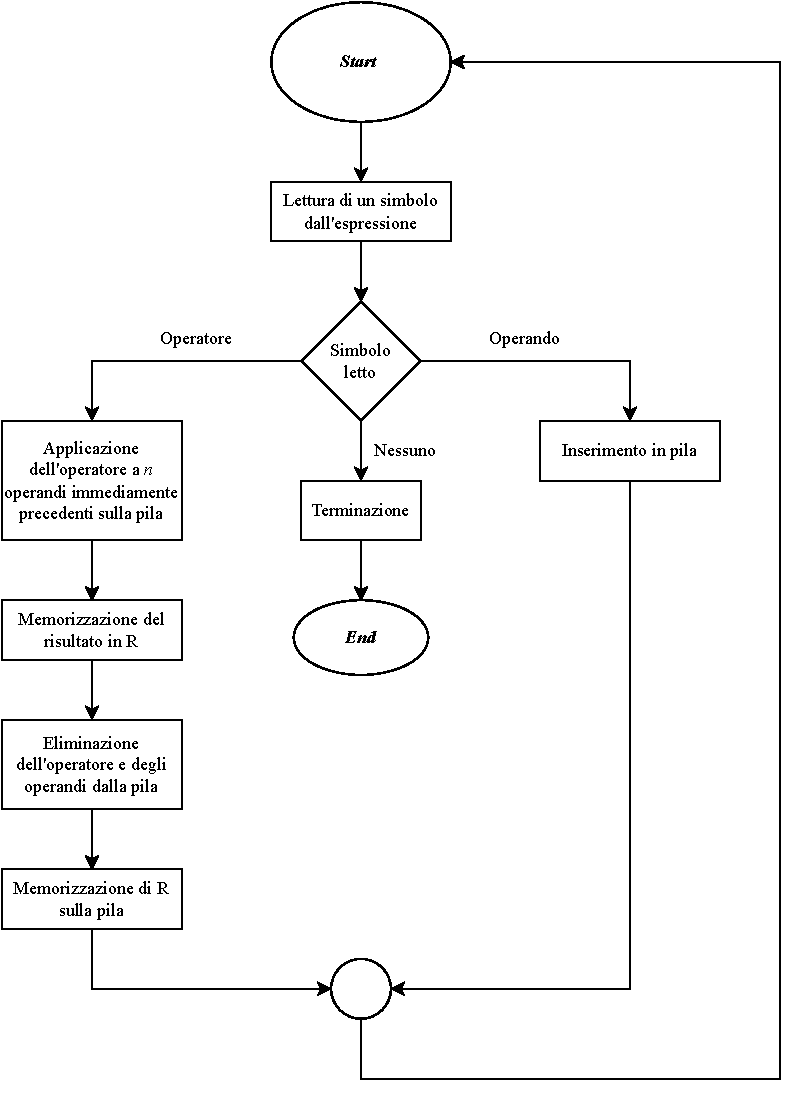
\includegraphics[width=\textwidth]{img/algoritmo_notazione_post-fissa.pdf}
		\caption{Algoritmo di valutazione nella notazione post-fissa.}
	\end{figure}\newpage

	\begin{figure}[!htp]
		\centering
		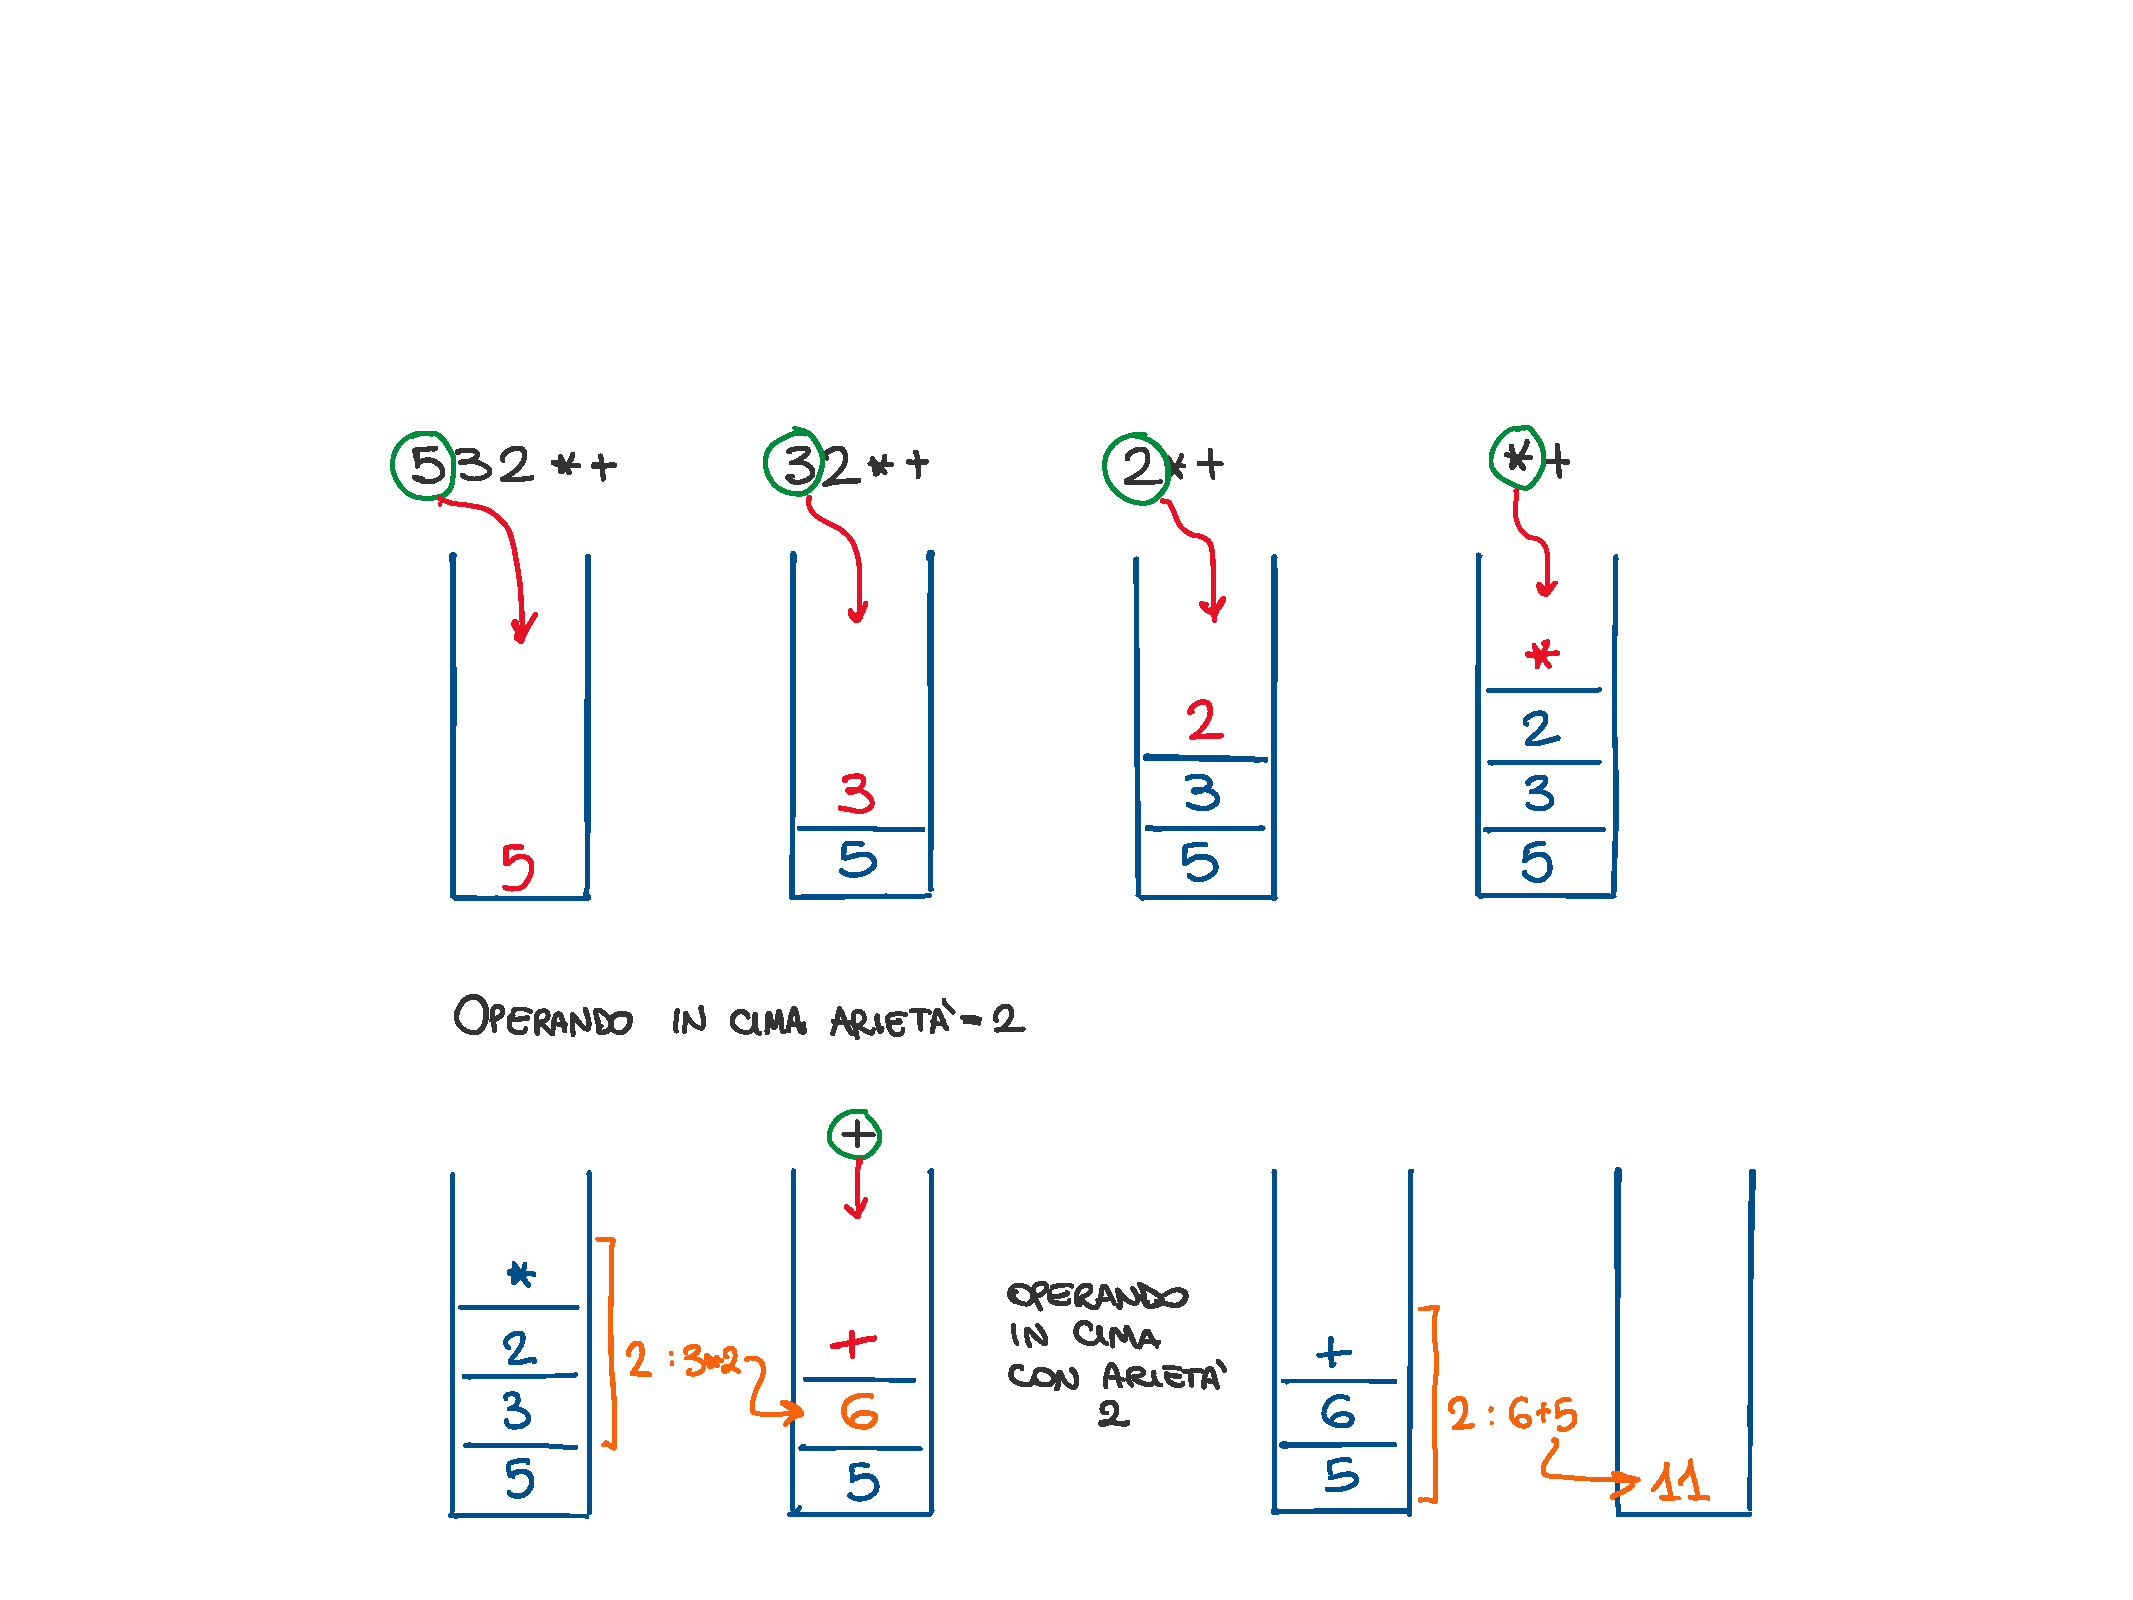
\includegraphics[width=\textwidth]{img/esempio_notazione_post-fissa.pdf}
		\caption{Esempio di applicazione dell'algoritmo di valutazione della notazione post-fissa.}
	\end{figure}\newpage
	
	\subsubsection{Notazione pre-fissa}\label{notazione pre-fissa}
	
	La notazione \textcolor{Red3}{\textbf{pre-fissa}} è \textbf{più semplice della in-fissa}, dal punto di vista della \textbf{computazione}, poiché:
	\begin{itemize}
		\item Non sono necessarie regole di precedenza
		\item Non sono necessarie regole di associatività
		\item Non sono necessarie parentesi
	\end{itemize}
	Viene anche concessa una rappresentazione uniforme per qualsiasi arietà di operatori\footnote{Arietà: numero di operandi a cui si applica.}.\newline
	
	\noindent
	A \textbf{differenza della notazione post-fissa}, l'\textbf{algoritmo} di valutazione è \textbf{più complicato} poiché è necessario contare gli operandi che vengono letti.\newline
	
	\noindent
	Per \textcolor{Green4}{\textbf{esempio}}, la notazione $*+ab+cd$ viene valutata da sinistra a destra usando una pila LIFO (\emph{Last In, First Out}). A differenza delle altre notazioni, in questo caso ogni volta che viene letto un operatore, è necessario contare gli operandi da leggere prima di eseguire il calcolo.\newline
	
	\noindent
	L'\textcolor{Red3}{\textbf{algoritmo di valutazione}} si articola in pochi passaggi. \textbf{Graficamente è possibile leggerlo nella prossima pagina}, mentre in forma scritta qui di seguito:
	\begin{enumerate}
		\item Lettura di un simbolo dall'espressione e inserimento in pila.
		
		\begin{enumerate}
			\item Se il simbolo letto è un operatore, inizializza il contatore $C$ con il numero di argomenti dell'operatore $\left(C_{op} = n\right)$ e torna al punto 1;
			
			\item Se il simbolo letto è un operando, decrementa il contatore $C$ di uno $\left(C_{op} = C_{op}-1\right)$ ($op$ è l'ultimo operatore inserito):
			
			\begin{enumerate}
				\item Se $C_{op} \ne 0$, torna al punto 1;
				
				\item Se $C_{op} = 0$ vengono eseguite le seguenti operazioni:
				
				\begin{enumerate}
					\item Applicazione dell'ultimo operatore agli operandi in cima alla pila;\newline
					memorizzazione del risultato in $R$;\newline
					eliminazione dell'operatore e degli operandi processati dalla pila;\newline
					memorizzazione del risultato $R$ sulla pila;
					
					\item Se non vi sono più simboli di operatore sulla pila, si salta al punto 2 (la fine);
					
					\item Inizializzazione del nuovo contatore: $C_{op} = n - m$ dove $n$ è l'arietà del nuovo operatore nella pila, il quale si trova in cima, e $m$ è il numero di operandi presenti nella pila sopra tale operatore;
					
					\item Ritorna al punto \emph{i}.
				\end{enumerate}
			\end{enumerate}
		\end{enumerate}
		
		\item Se la sequenza da leggere non è vuota torna all'1.
	\end{enumerate}\newpage
	
	\begin{figure}[!htp]
		\centering
		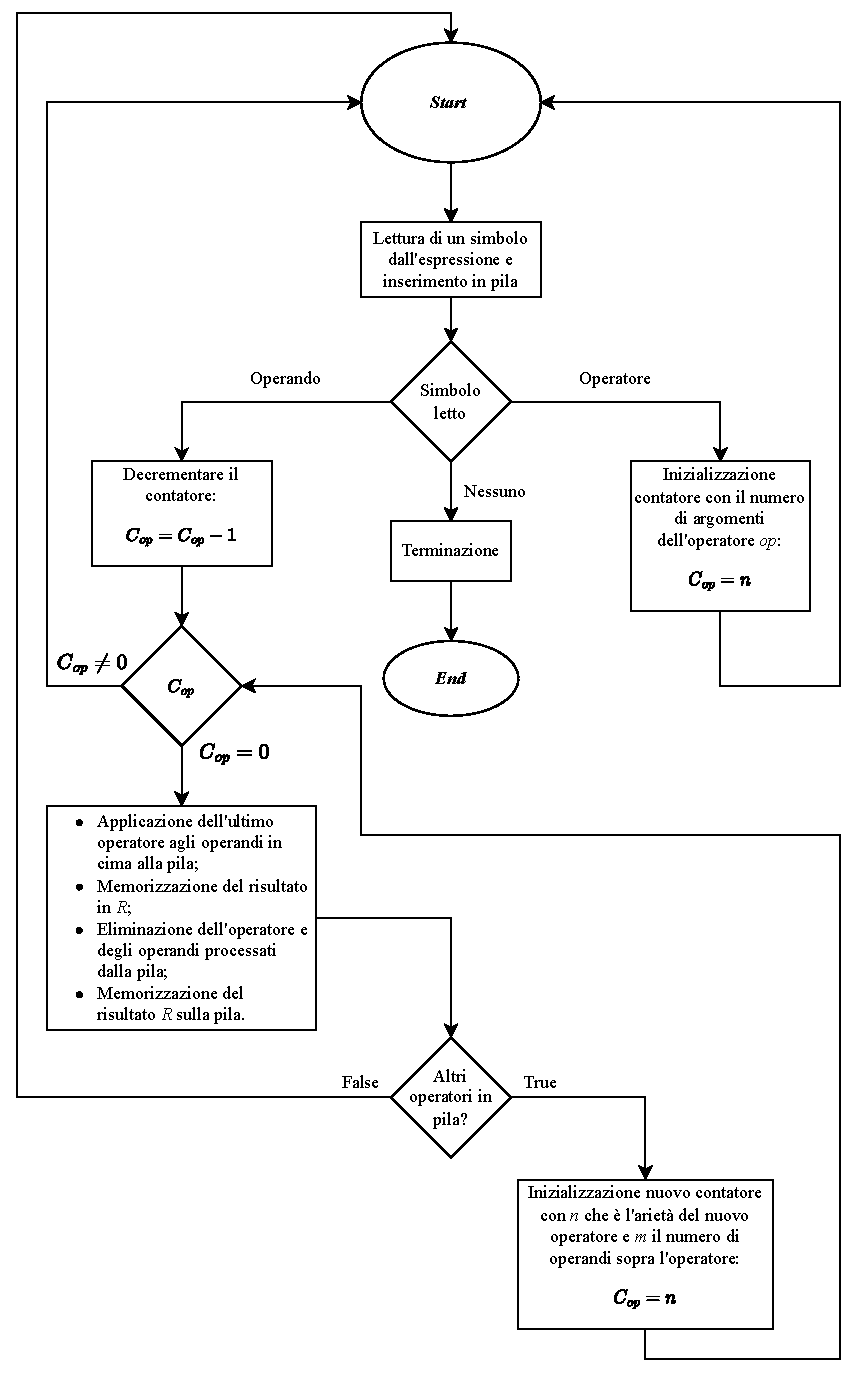
\includegraphics[width=\textwidth]{img/algoritmo_notazione_pre-fissa.pdf}
		\caption{Algoritmo di valutazione nella notazione post-fissa.}
	\end{figure}\newpage
	
	\begin{figure}[!htp]
		\centering
		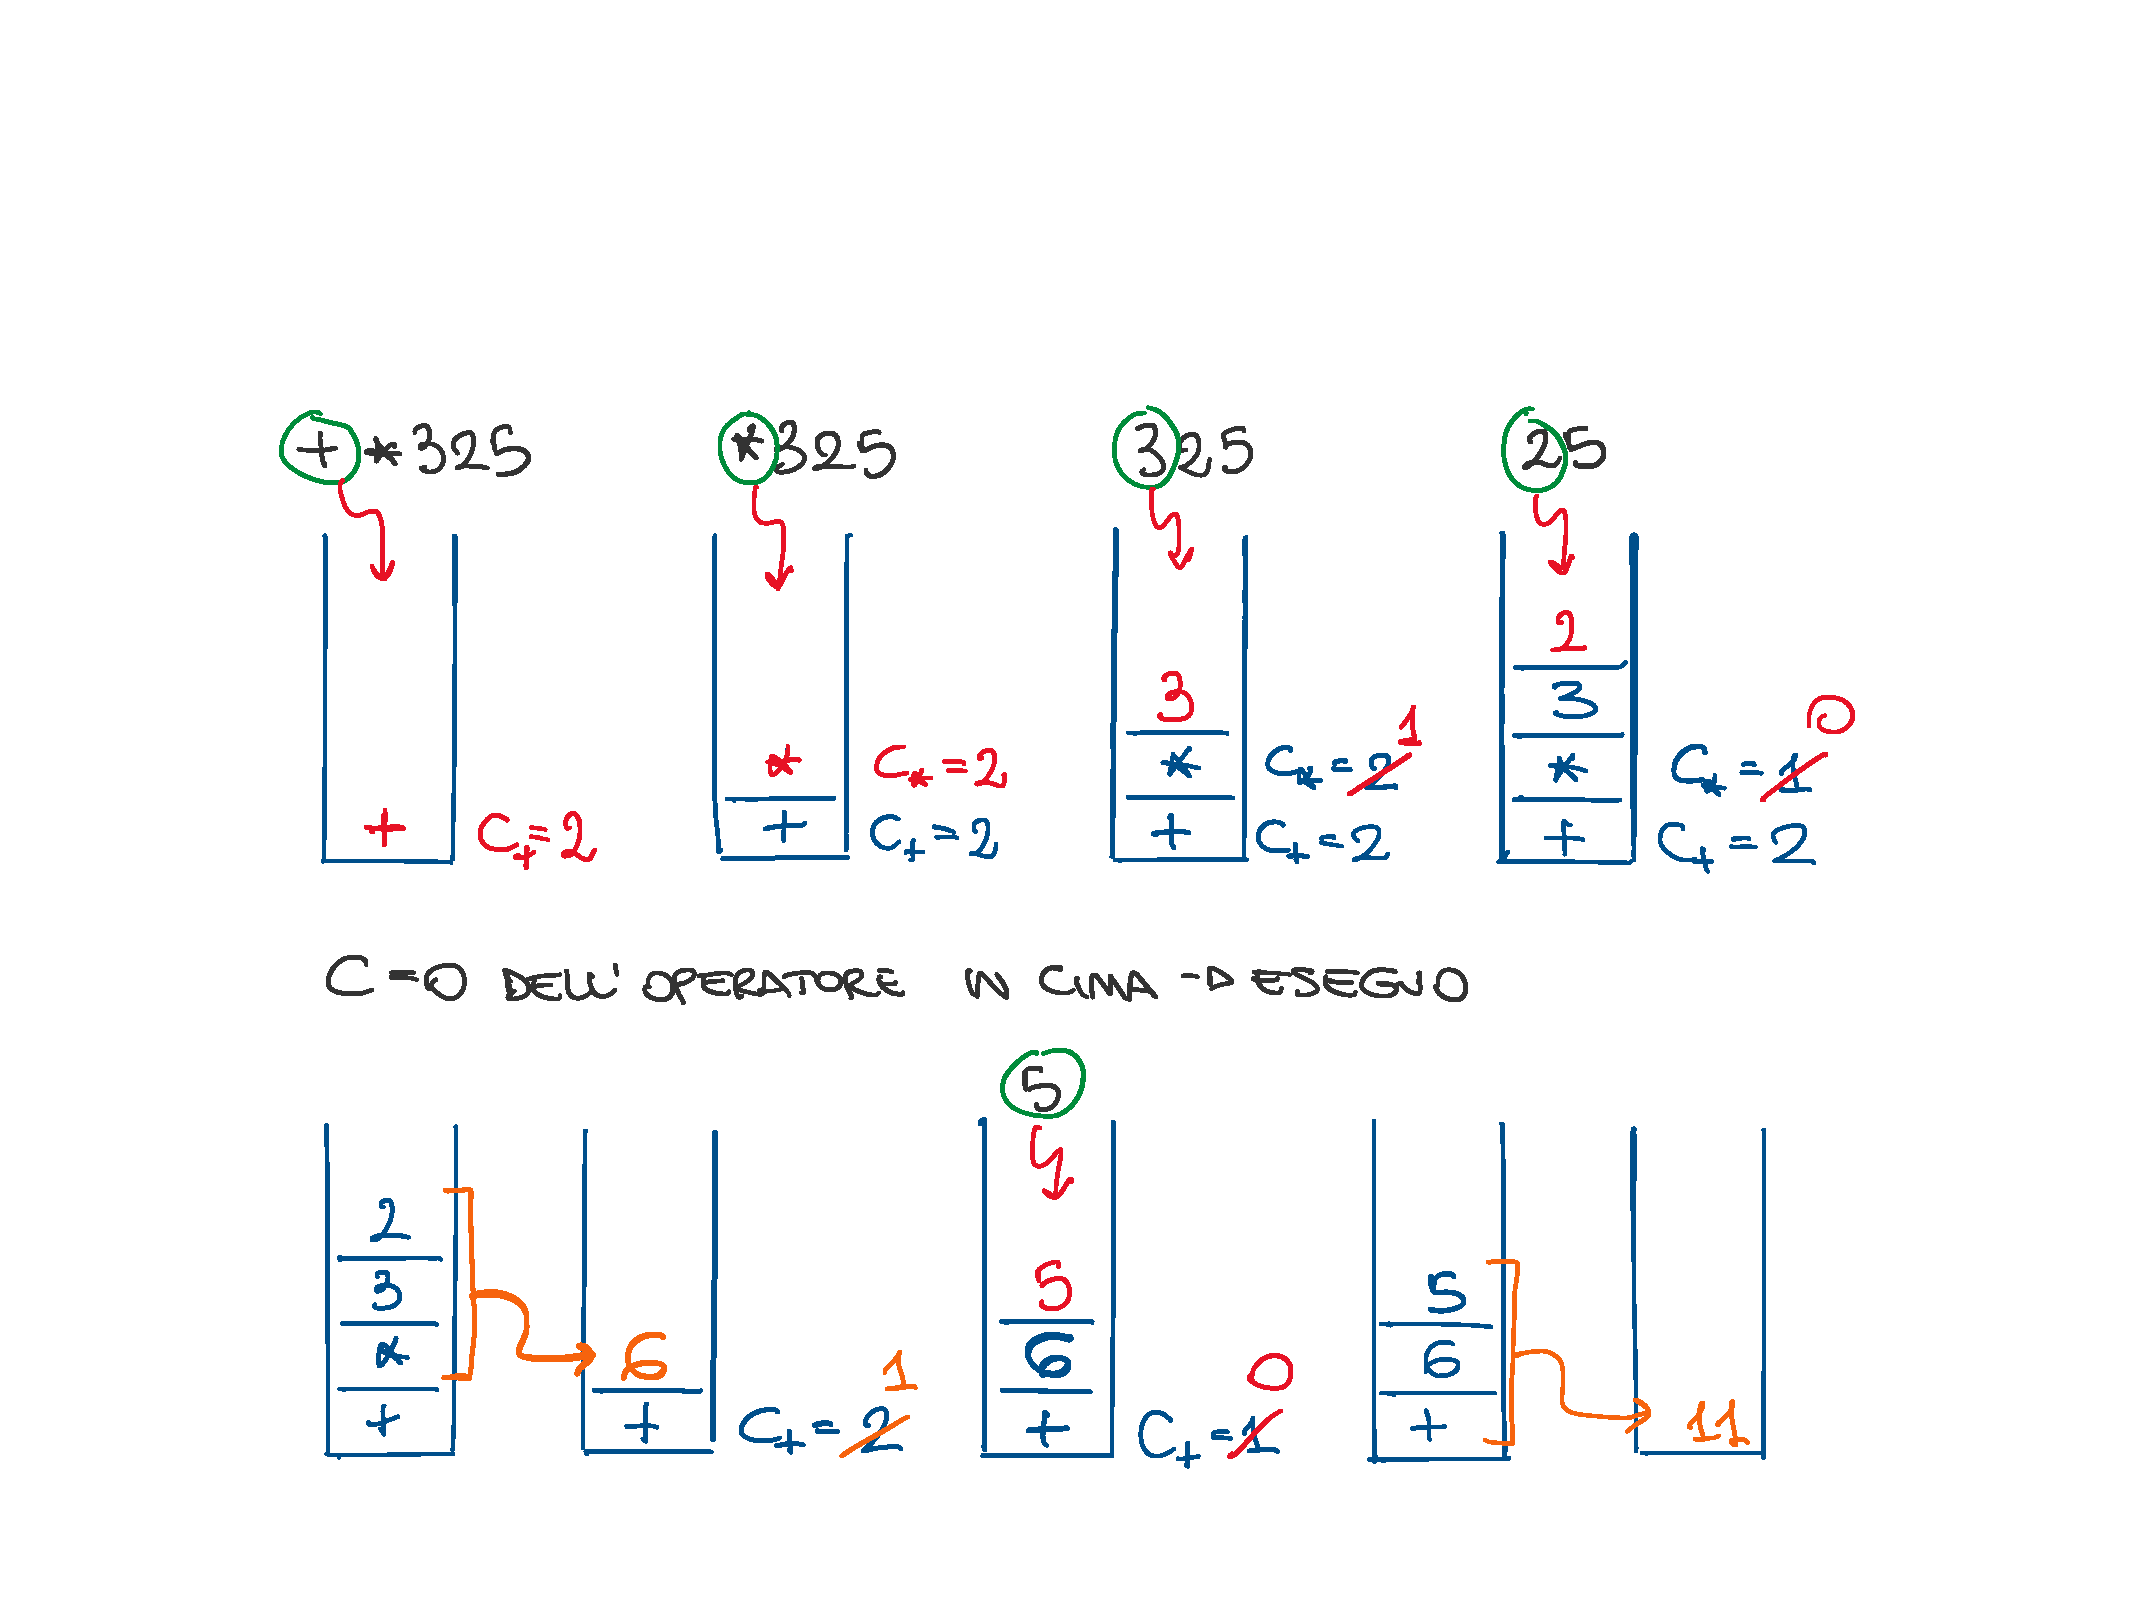
\includegraphics[width=\textwidth]{img/esempio_notazione_pre-fissa.pdf}
		\caption{Esempio di applicazione dell'algoritmo di valutazione della notazione pre-fissa.}
	\end{figure}\newpage
	
	\subsubsection{Notazione in-fissa}\label{notazione in-fissa}
	
	La notazione \textcolor{Red3}{\textbf{in-fissa}} è la \textbf{notazione più utilizzata in matematica} e nei linguaggi di programmazione come zucchero sintattico. Inoltre, è quella che consente una lettura più intuitiva ma che richiede maggiori specifiche.\newline
	
	\noindent
	Per \textcolor{Green4}{\textbf{esempio}}, considerando $15-5-3$, a seconda dell'operazione che viene eseguita per prima, cambia il risultato.\newline
	
	\noindent
	L'algoritmo di valutazione della notazione in-fissa non è così semplice come i precedenti. Infatti, a causa di alcune regole, chiamate di \textbf{precedenza} e \textbf{associatività}, e alla presenza di alcune regole, non è possibile valutare l'espressione con una semplice scansione da sinistra a destra o viceversa.\newline
	
	\noindent
	\begin{boxdef}
		Con \textcolor{Red3}{\textbf{regole di precedenza}} si intende: \textbf{le regole di precedenza di un operatore per la valutazione di un'espressione, definisce l'ordine in cui operatori \dquotes{adiacenti} a diversi livelli di precedenza vengono valutati}.
	\end{boxdef}

	\noindent
	Anche se ogni linguaggio differisce per le priorità assegnate agli operatori, l'importante è che vengano stabilite a priori. Per \textcolor{Green4}{\textbf{esempio}}, un tipico livello di precedenza è dato da: (1) parentesi, (2) operatori unari, (3) elevazione a potenza, (4) moltiplicazione e divisione, (5) somma e sottrazione.\newline
	
	\noindent
	\begin{boxdef}
		Con \textcolor{Red3}{\textbf{regole di associatività}} si intende: \textbf{le regole di associatività per la valutazione delle espressioni definiscono l'ordine con cui operatori allo stesso livello di precedenza vengono valutati}.
	\end{boxdef}

	\noindent
	Per \textcolor{Green4}{\textbf{esempio}}, delle tipiche regole di associatività sono: da sinistra verso destra; a volte operatori unitari associano da destra; in alcuni linguaggi tutti gli operatori hanno lo stesso livello di precedenza e associano da destra; le regole di precedenza e associatività possono essere sovrascritte usando le parentesi.\newline
	Un altro \textcolor{Green4}{\textbf{esempio}} $a+b-c+d$ restituisce valori diversi a seconda che si associ da destra o da sinistra.\newpage
	
	\subsection{Valutazione delle espressioni}\label{valutazione delle espressioni}
	
	La rappresentazione interna della espressioni consiste in una \textbf{rappresentazione ad albero} (\emph{abstract syntax tree}), dove i \textbf{nodi interni} sono \textbf{operatori} mentre le foglie sono valori (operandi elementari). Ogni nodo interno ha come figli gli alberi che rappresentano le espressioni a cui l'operatore si applica.\newline
	
	\noindent
	In altre parole, l'\textbf{albero fornisce la struttura dell'espressione}, ovvero:
	\begin{itemize}
		\item \textcolor{Green4}{\textbf{Aspetto positivo:}} elimina eventuali ambiguità legate a precedenze e associatività;
		\item \textcolor{Red3}{\textbf{Aspetto negativo:}} non dà informazioni riguardanti l'ordine di valutazione dell'espressione.
	\end{itemize}
	
	\noindent
	A causa delle eventuali ambiguità sulle espressioni, nasce il \textcolor{Red3}{\textbf{problema dell'ordine di valutazione}}, il quale è prettamente informatico. Infatti, la presenza di alcune caratteristiche influenzano il risultato:
	\begin{itemize}
		\item \textbf{Operandi non definiti}. Se esistono degli \textbf{operandi non definiti}, può accadere che l'espressione venga valutata solo con un preciso ordine. Per esempio, con l'espressione $\left(a == 0 ? b : b/a\right)$, è chiaro che $b/a$ può essere una divisione per $0$, quindi non definita. Tuttavia è necessario che venga valutata solo per divisioni diverse da zero, quindi un linguaggio di programmazione può essere:
		\begin{itemize}
			\item \textbf{Valutazione \textcolor{Red3}{\emph{lazy}}} (o corto circuito), ovvero gli operandi vengono valutati solo quando è necessario, quindi quando l'espressione è sempre definita.
			
			\item \textbf{Valutazione \textcolor{Red3}{\emph{eager}}}, ovvero gli operandi vengono valutati sempre.
		\end{itemize}
		Un ottimo \textcolor{Green4}{\textbf{esempio}} per comprendere la distinzione: \href{https://www.tutorialspoint.com/functional_programming_with_java/functional_programming_with_java_evaluation.htm}{link}
		
		\item \textbf{Effetti collaterali} (\emph{side effects}). Sono \textbf{effetti non legati all'oggetto di cui vi è la manipolazione}, per esempio: la valutazione di un'espressione provoca un cambiamento della memoria; una funzione modifica i propri parametri o modifica variabili non locali. Un \textcolor{Green4}{\textbf{esempio}} più tangibile è $\left(\left(a+f\left(b\right)\right) * \left(c+f\left(b\right)\right)\right)$ con la funzione $f\left(b\right)$ definita come $b++$ e l'espressione ritorna valori diversi a seconda dell'ordine di valutazione.
		
		\item \textbf{Aritmetica finita}. Nelle macchine l'\textbf{aritmetica è limitata dall'architettura, quindi i numeri non sono infiniti ed esiste un massimo numero rappresentabile}. I \textbf{problema di valutazione} avviene quando le espressioni coinvolgono tale numero.\newline
		Per \textcolor{Green4}{\textbf{esempio}} se viene eseguita una somma prima di una differenza, è possibile cambiare il risultato se la somma calcola un numero maggiore del massimo numero rappresentabile.
	\end{itemize}\newpage
	
	\subsection{Semantica delle espressioni}
	
	La \textcolor{Red3}{\textbf{semantica delle espressioni}} di un linguaggio imperativo $IMP$ cerca di descrivere la semantica senza interessarsi della grammatica, la quale include tutte le regole di associatività e precedenza. Quindi, vengono ignorante anche le parentesi, nonostante tutte queste regole rendono un'espressione chiara e non ambigua.\newline
	
	\noindent
	L'aspetto d'interesse è la \textbf{struttura induttiva} e non la struttura sintattica. Per questo motivo si introducono alcune definizione teoriche:
	\begin{boxdef}
		Le \textcolor{Red3}{\textbf{espressioni}} $\mathcal{E}$ è un \textbf{insieme di (alberi di valutazione) di espressioni valutate ad intero o booleano}. Gli elementi solitamente vengono rappresentati con la lettera $e$.
	\end{boxdef}
	\begin{boxdef}
		I \textcolor{Red3}{\textbf{numeri}} $\mathcal{N}$ è un \textbf{insieme di numeri reali nella macchina}. Gli elementi solitamente vengono rappresentati con le lettere $m$, $n$ o $p$.
	\end{boxdef}
	\begin{boxdef}
		I \textcolor{Red3}{\textbf{booleani}} $\mathcal{B}$ è un \textbf{insieme di valori booleani}. Composto solo da \textsf{true} e \textsf{false}. Gli elementi solitamente vengono rappresentati con la lettera $t$.
	\end{boxdef}
	
	\noindent
	Questi insiemi vengono usati per definire il \textcolor{Red3}{\textbf{sistema di transizione}}:
	\begin{equation*}
		\Gamma = \mathcal{E}, \hspace{2em} T = \mathcal{N} \cup \mathcal{B}, \hspace{2em} \mathrm{op}\in\left\{+,-,*,=\right\} \hspace{1em} \mathrm{bop} \in \left\{=, or\right\}
	\end{equation*}
	\begin{itemize}
		\item $\Gamma$ rappresenta l'insieme delle configurazioni;
		\item $\mathcal{E}$ rappresenta l'insieme delle espressioni da valutare;
		\item $T$ rappresenta l'insieme delle configurazioni terminali;
		\item $\mathrm{op}$ rappresenta l'insieme delle operazioni ammesse;
		\item $\mathrm{bop}$ rappresenta una metavariabile.
	\end{itemize}
	Quindi, viene definito l'insieme delle configurazioni come l'insieme delle espressioni da valutare $\left(\Gamma = \mathcal{E}\right)$; l'insieme delle configurazioni terminali sono un tutti i valori numerici e booleani $\left(T = \mathcal{N} \cup \mathcal{B}\right)$.\newpage
	
	\subsection{Regole di transizione}\label{regole di transizione}
	
	Si espongono qua di seguito le \textcolor{Red3}{\textbf{regole di transizione}}. Si tenga conto che con \textbf{bop} in grassetto si identifica il simbolo sintattico di un'operazione e con bop normale si identifica il simbolo dell'operazione nella macchina sottostante.\newline
	
	\noindent
	Si introducono le prime tre \textbf{regole necessarie per \underline{valutare espressioni aritmetiche}}:
	\begin{itemize}
		\item È un \underline{assioma} e \textbf{valuta l'espressione sintattica contenente un operatore aritmetico nel valore che esso rappresenta}. Per esempio, l'espressione $3+5$ viene valutata letteralmente come il valore $3$, l'operazione di somma $+$ e il valore $5$.
		\begin{figure}[!htp]
			\centering
			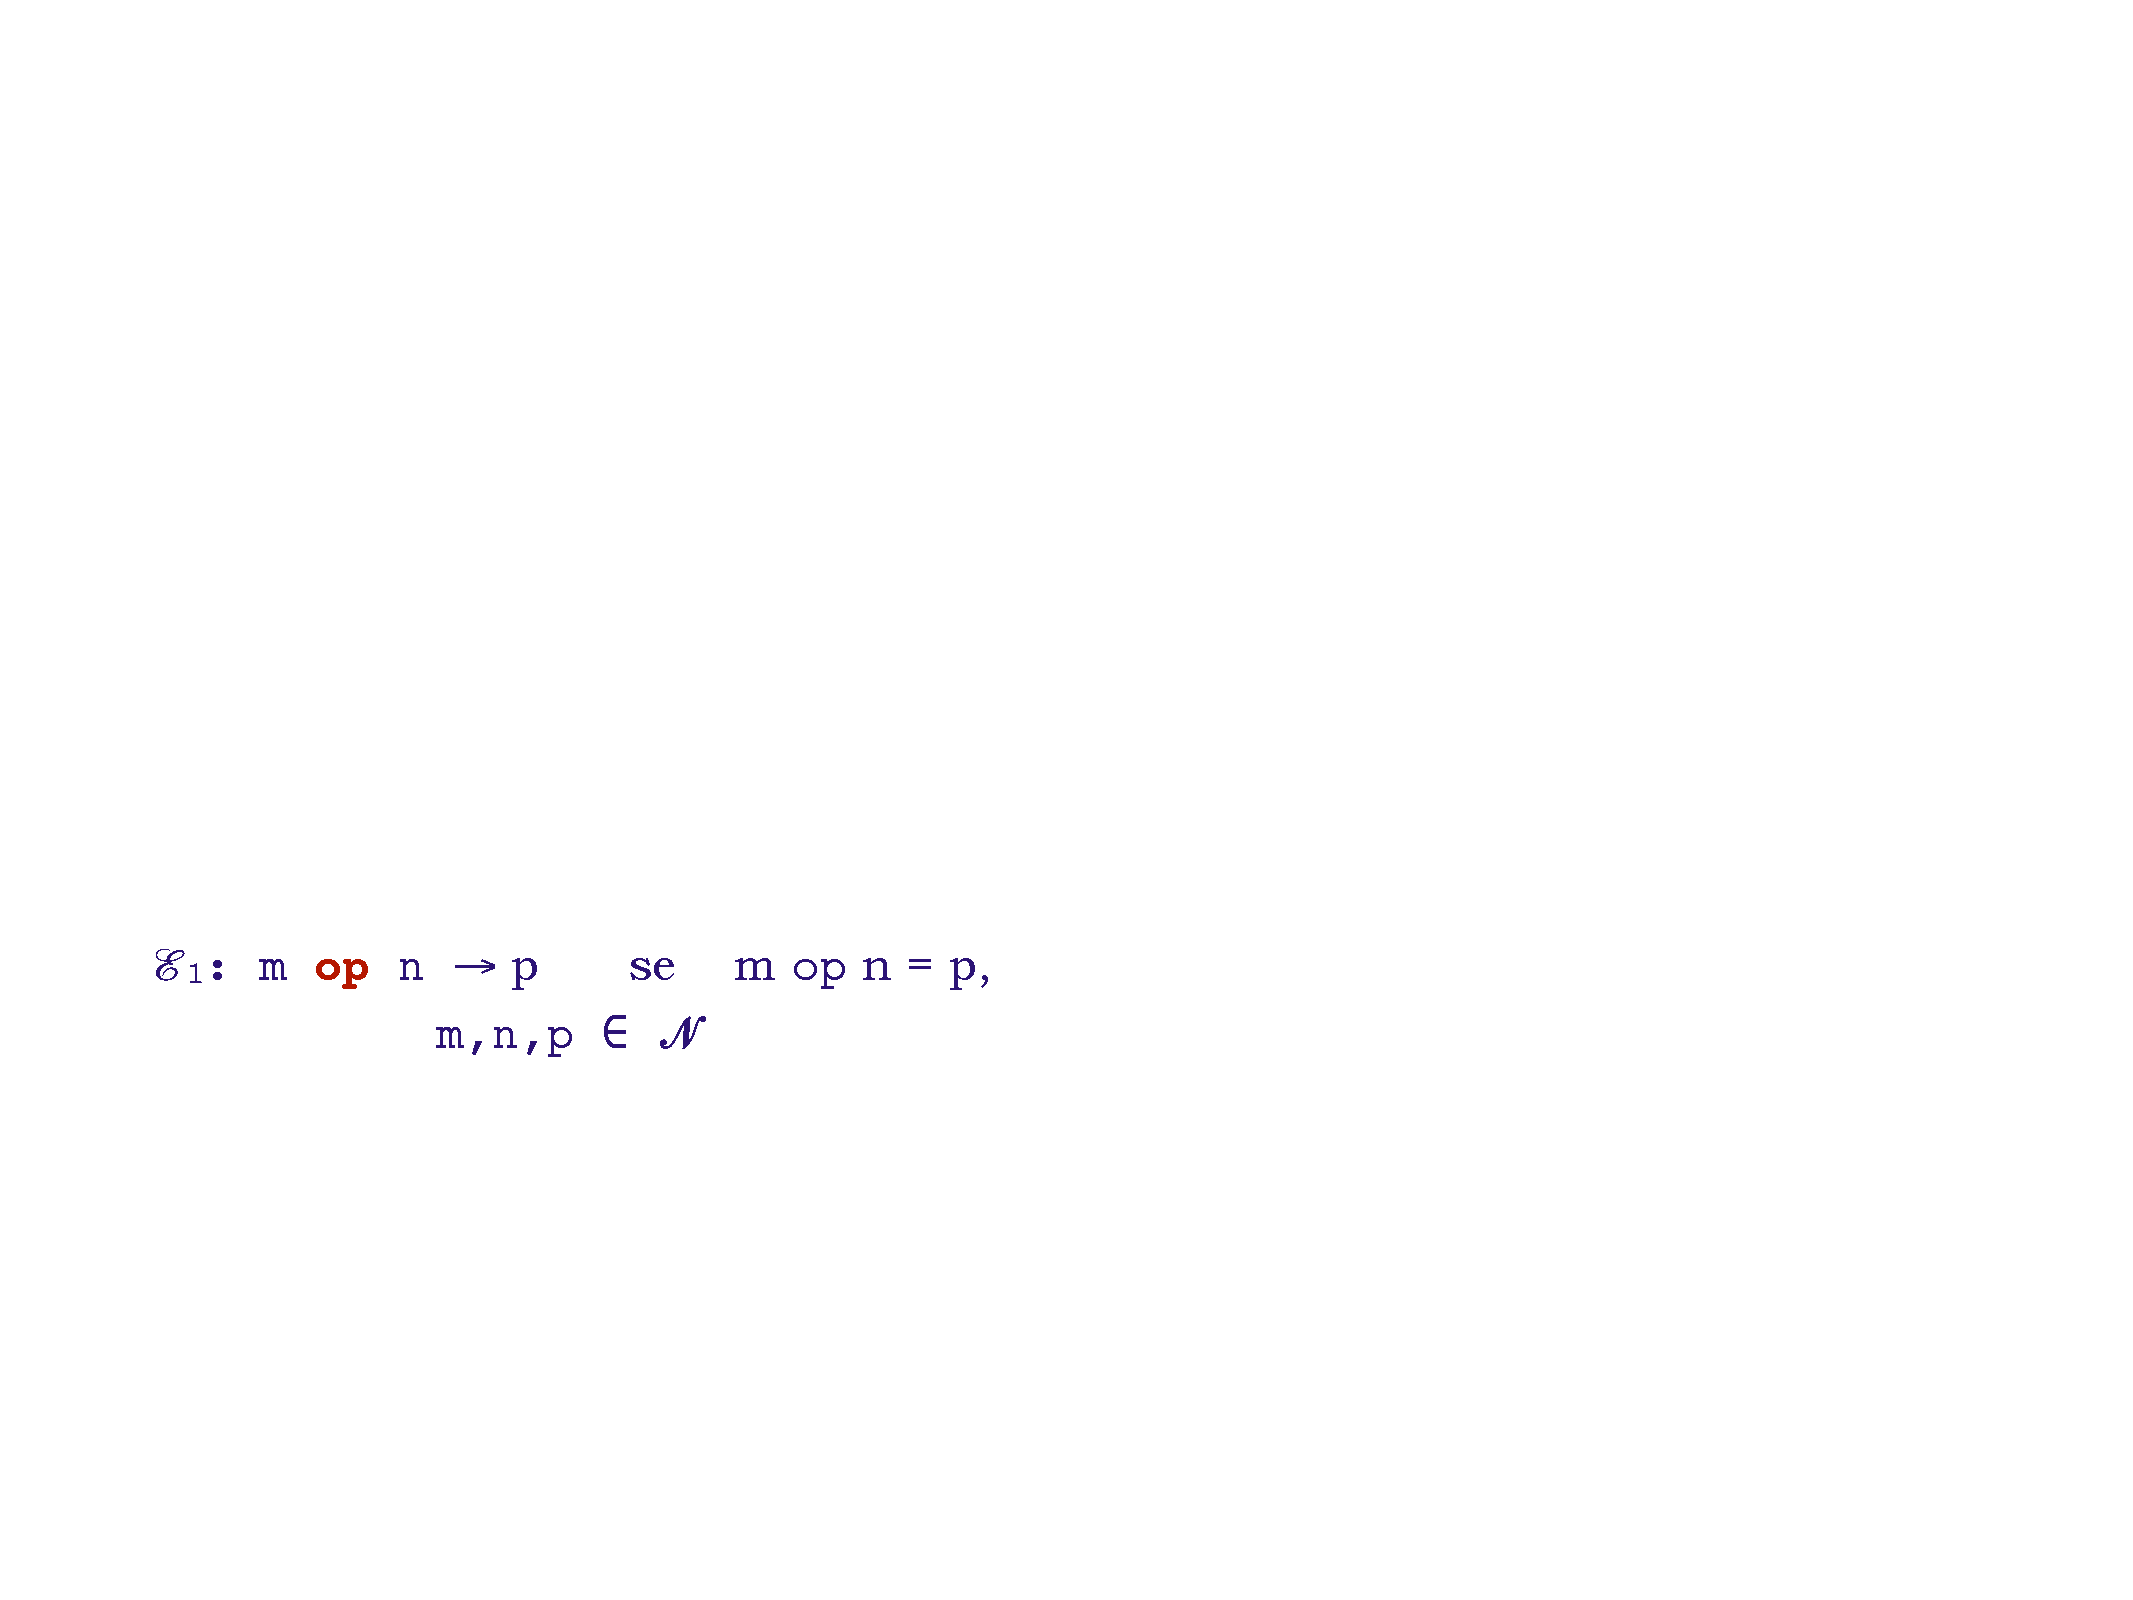
\includegraphics[width=.65\textwidth]{img/regola_transizione-1.pdf}
		\end{figure}
		
		\item È una \underline{regola induttiva} e indica che \textbf{se gli operandi non sono valori primitivi allora è necessario valutarli}.
		\begin{figure}[!htp]
			\centering
			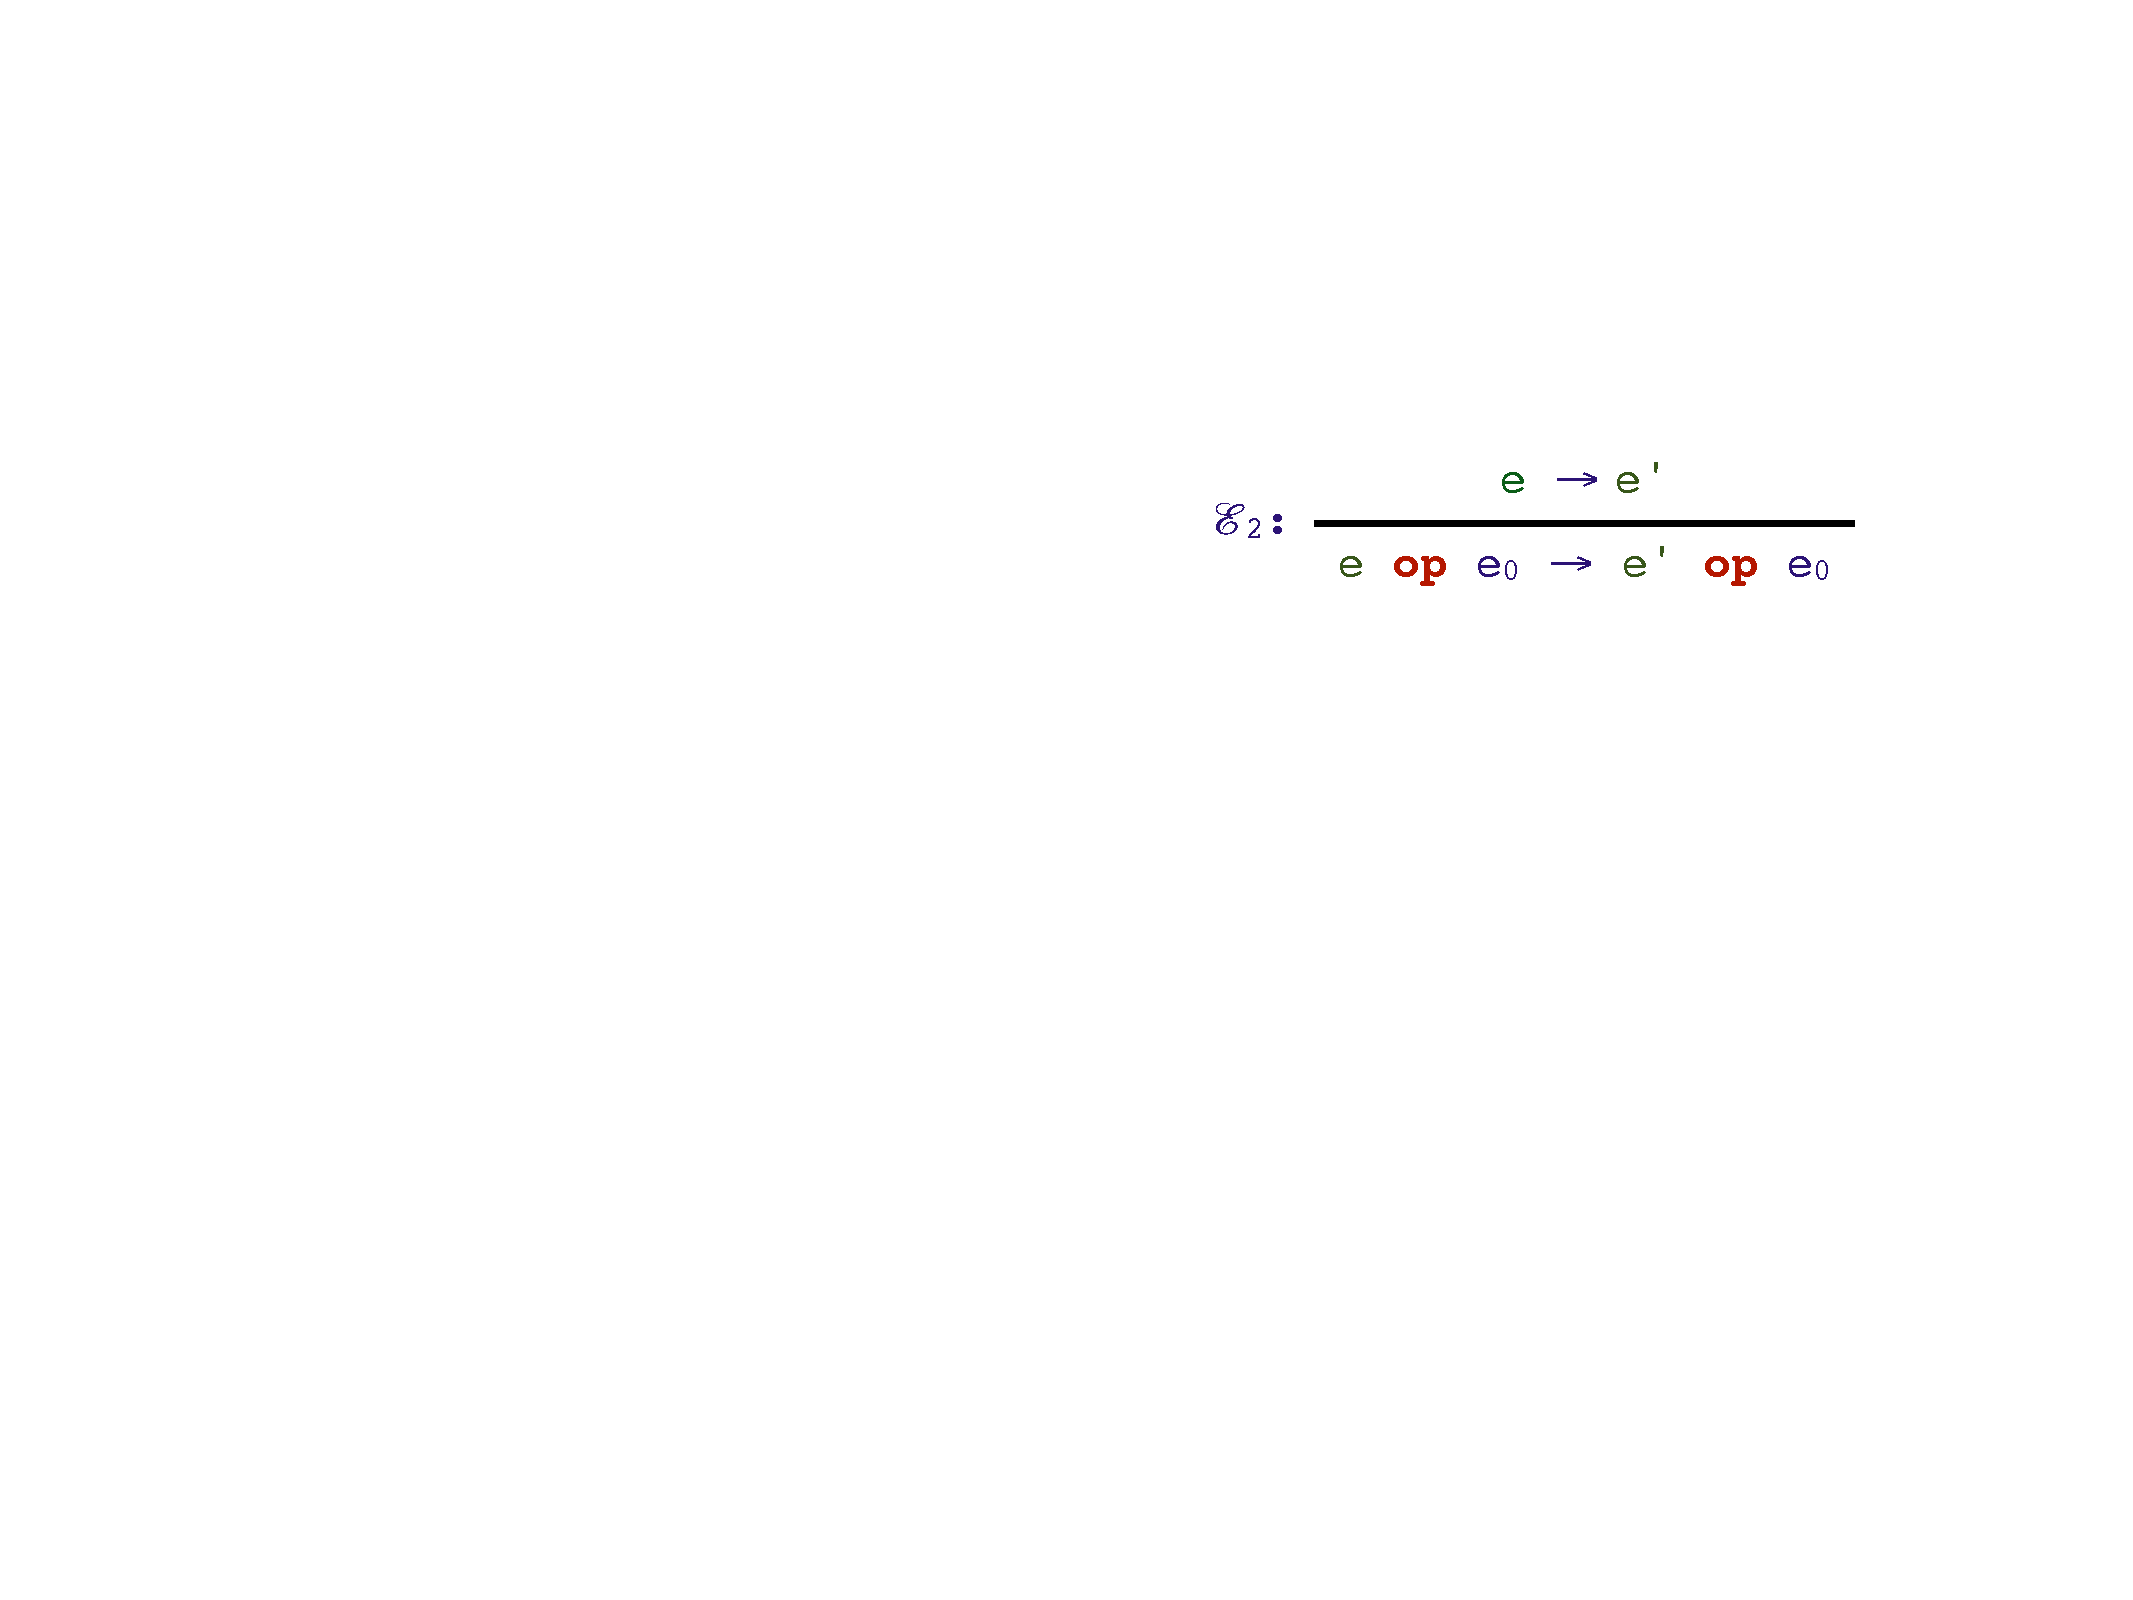
\includegraphics[width=.65\textwidth]{img/regola_transizione-2.pdf}
		\end{figure}
		
		\item La regola stabilisce che \textbf{nel momento in cui l'operando a sinistra è un valore allora è possibile iniziare a valutare l'operando a destra}. Ovviamente se anche l'operatore a destra è un valore allora si ricade nella prima regola ed è possibile restituire il valore finale.
		\begin{figure}[!htp]
			\centering
			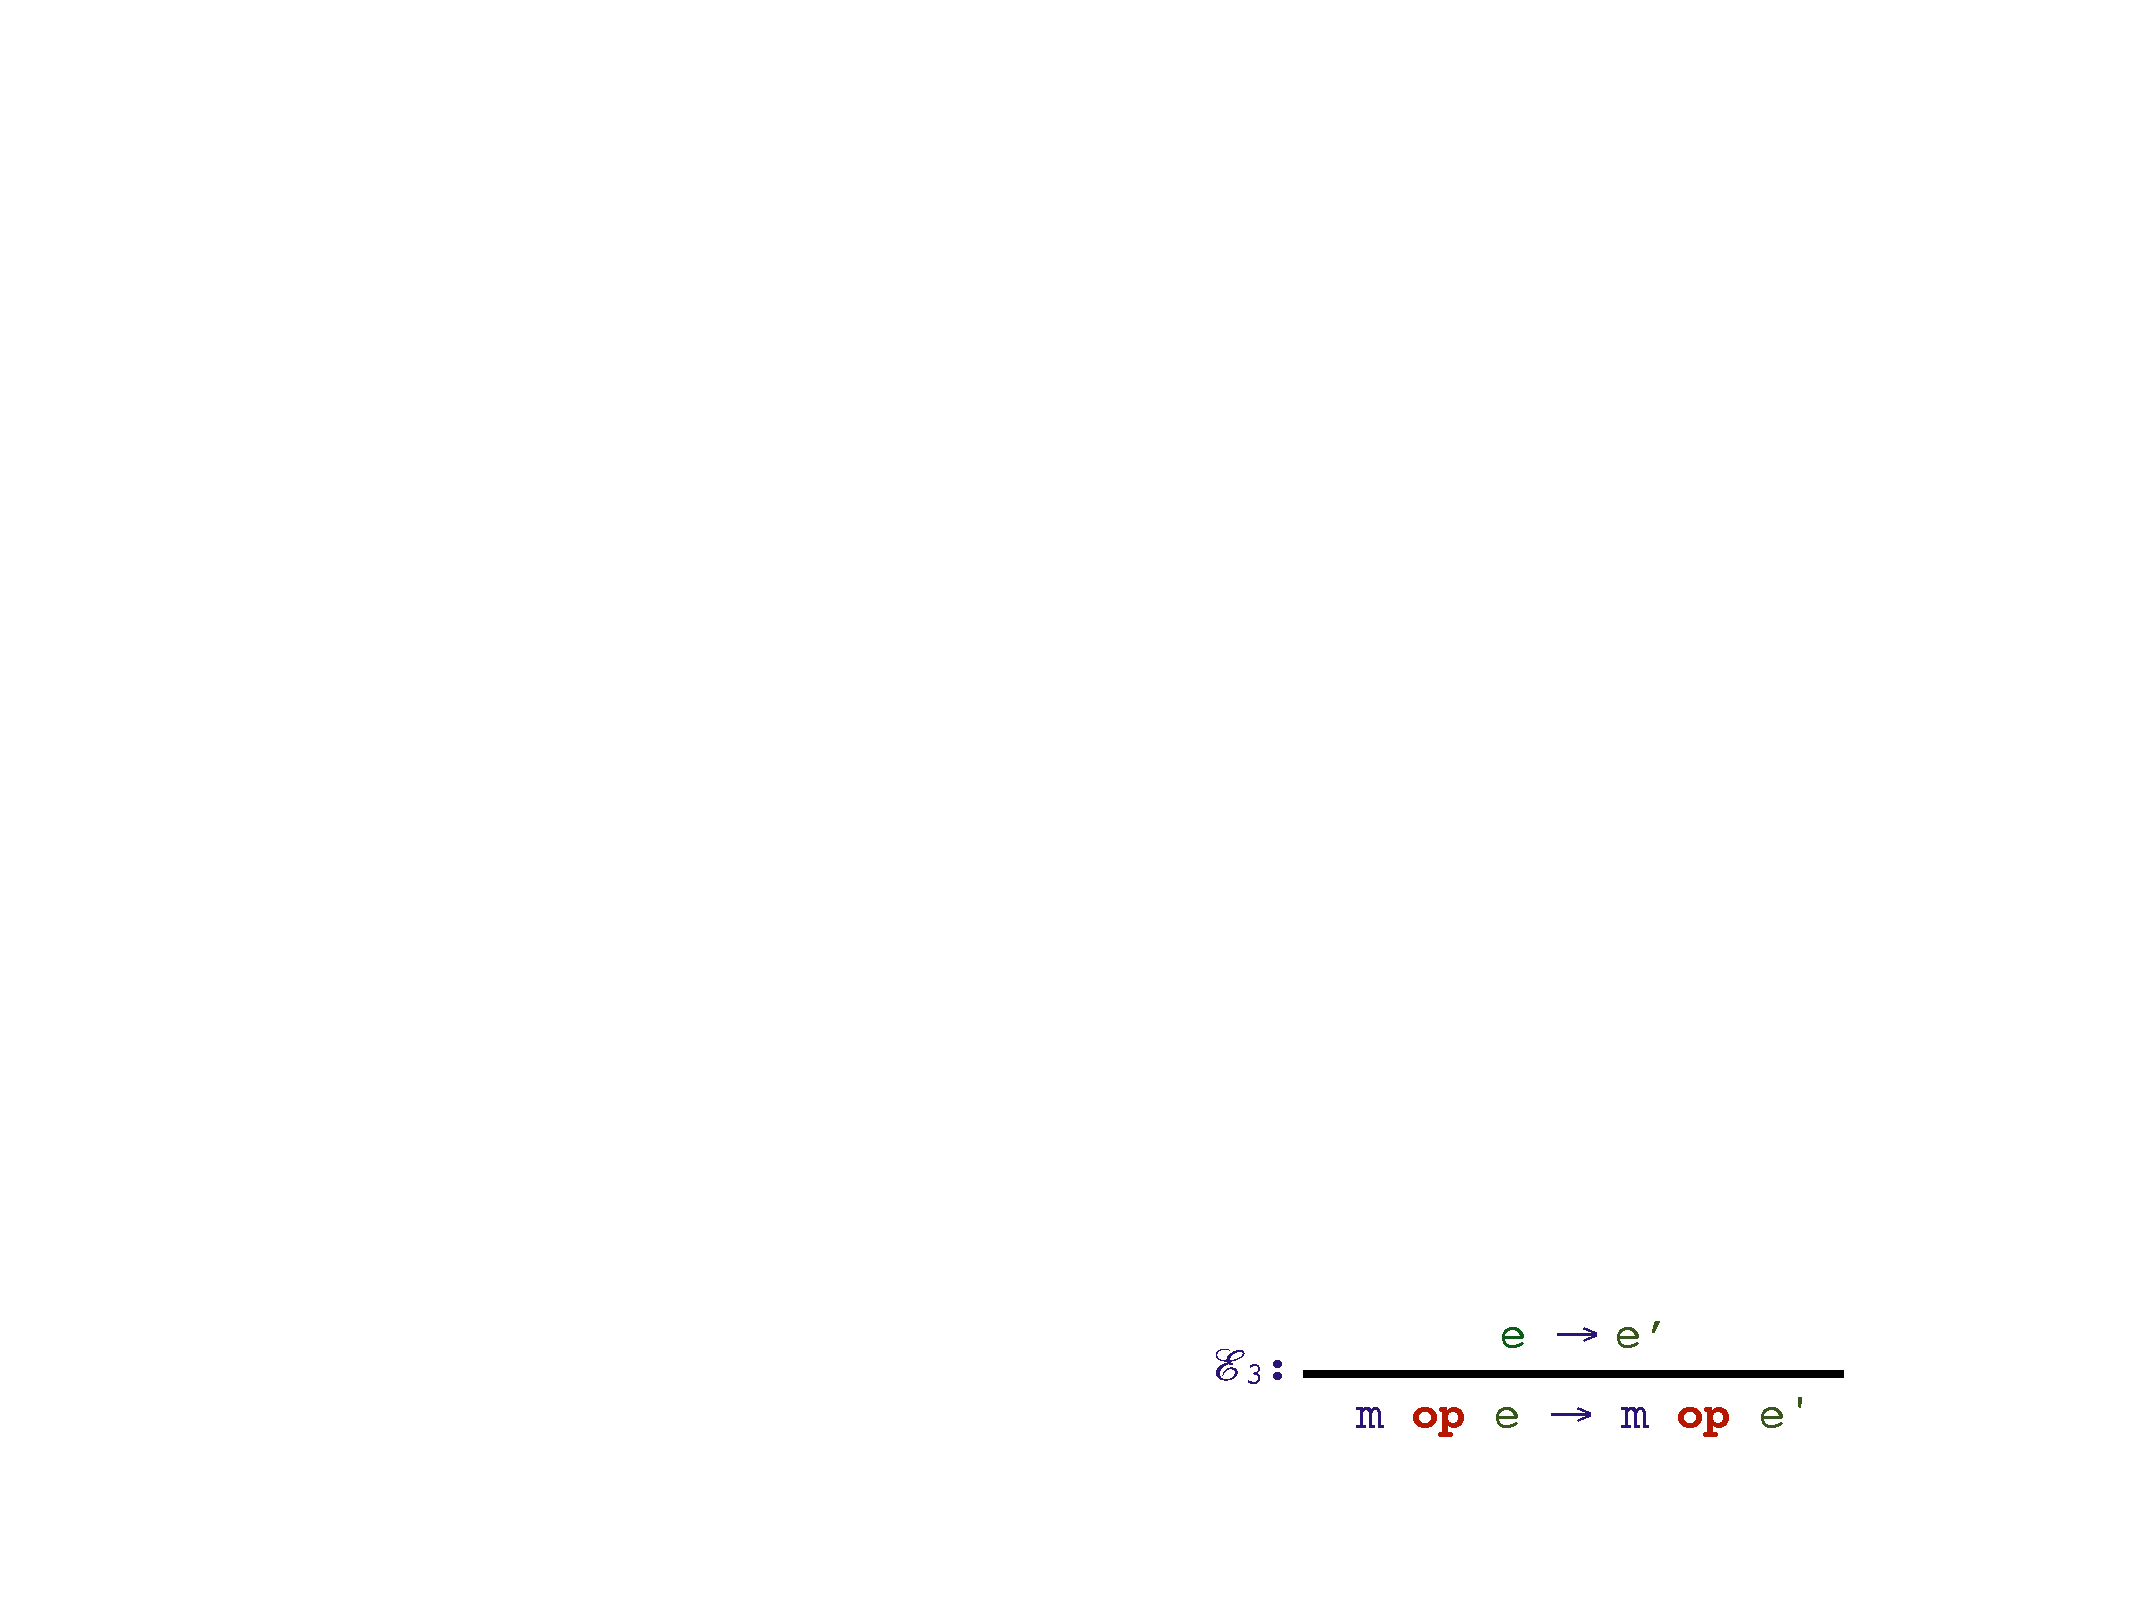
\includegraphics[width=.65\textwidth]{img/regola_transizione-3.pdf}
		\end{figure}
	\end{itemize}\newpage
	
	\begin{figure}[!htp]
		\centering
		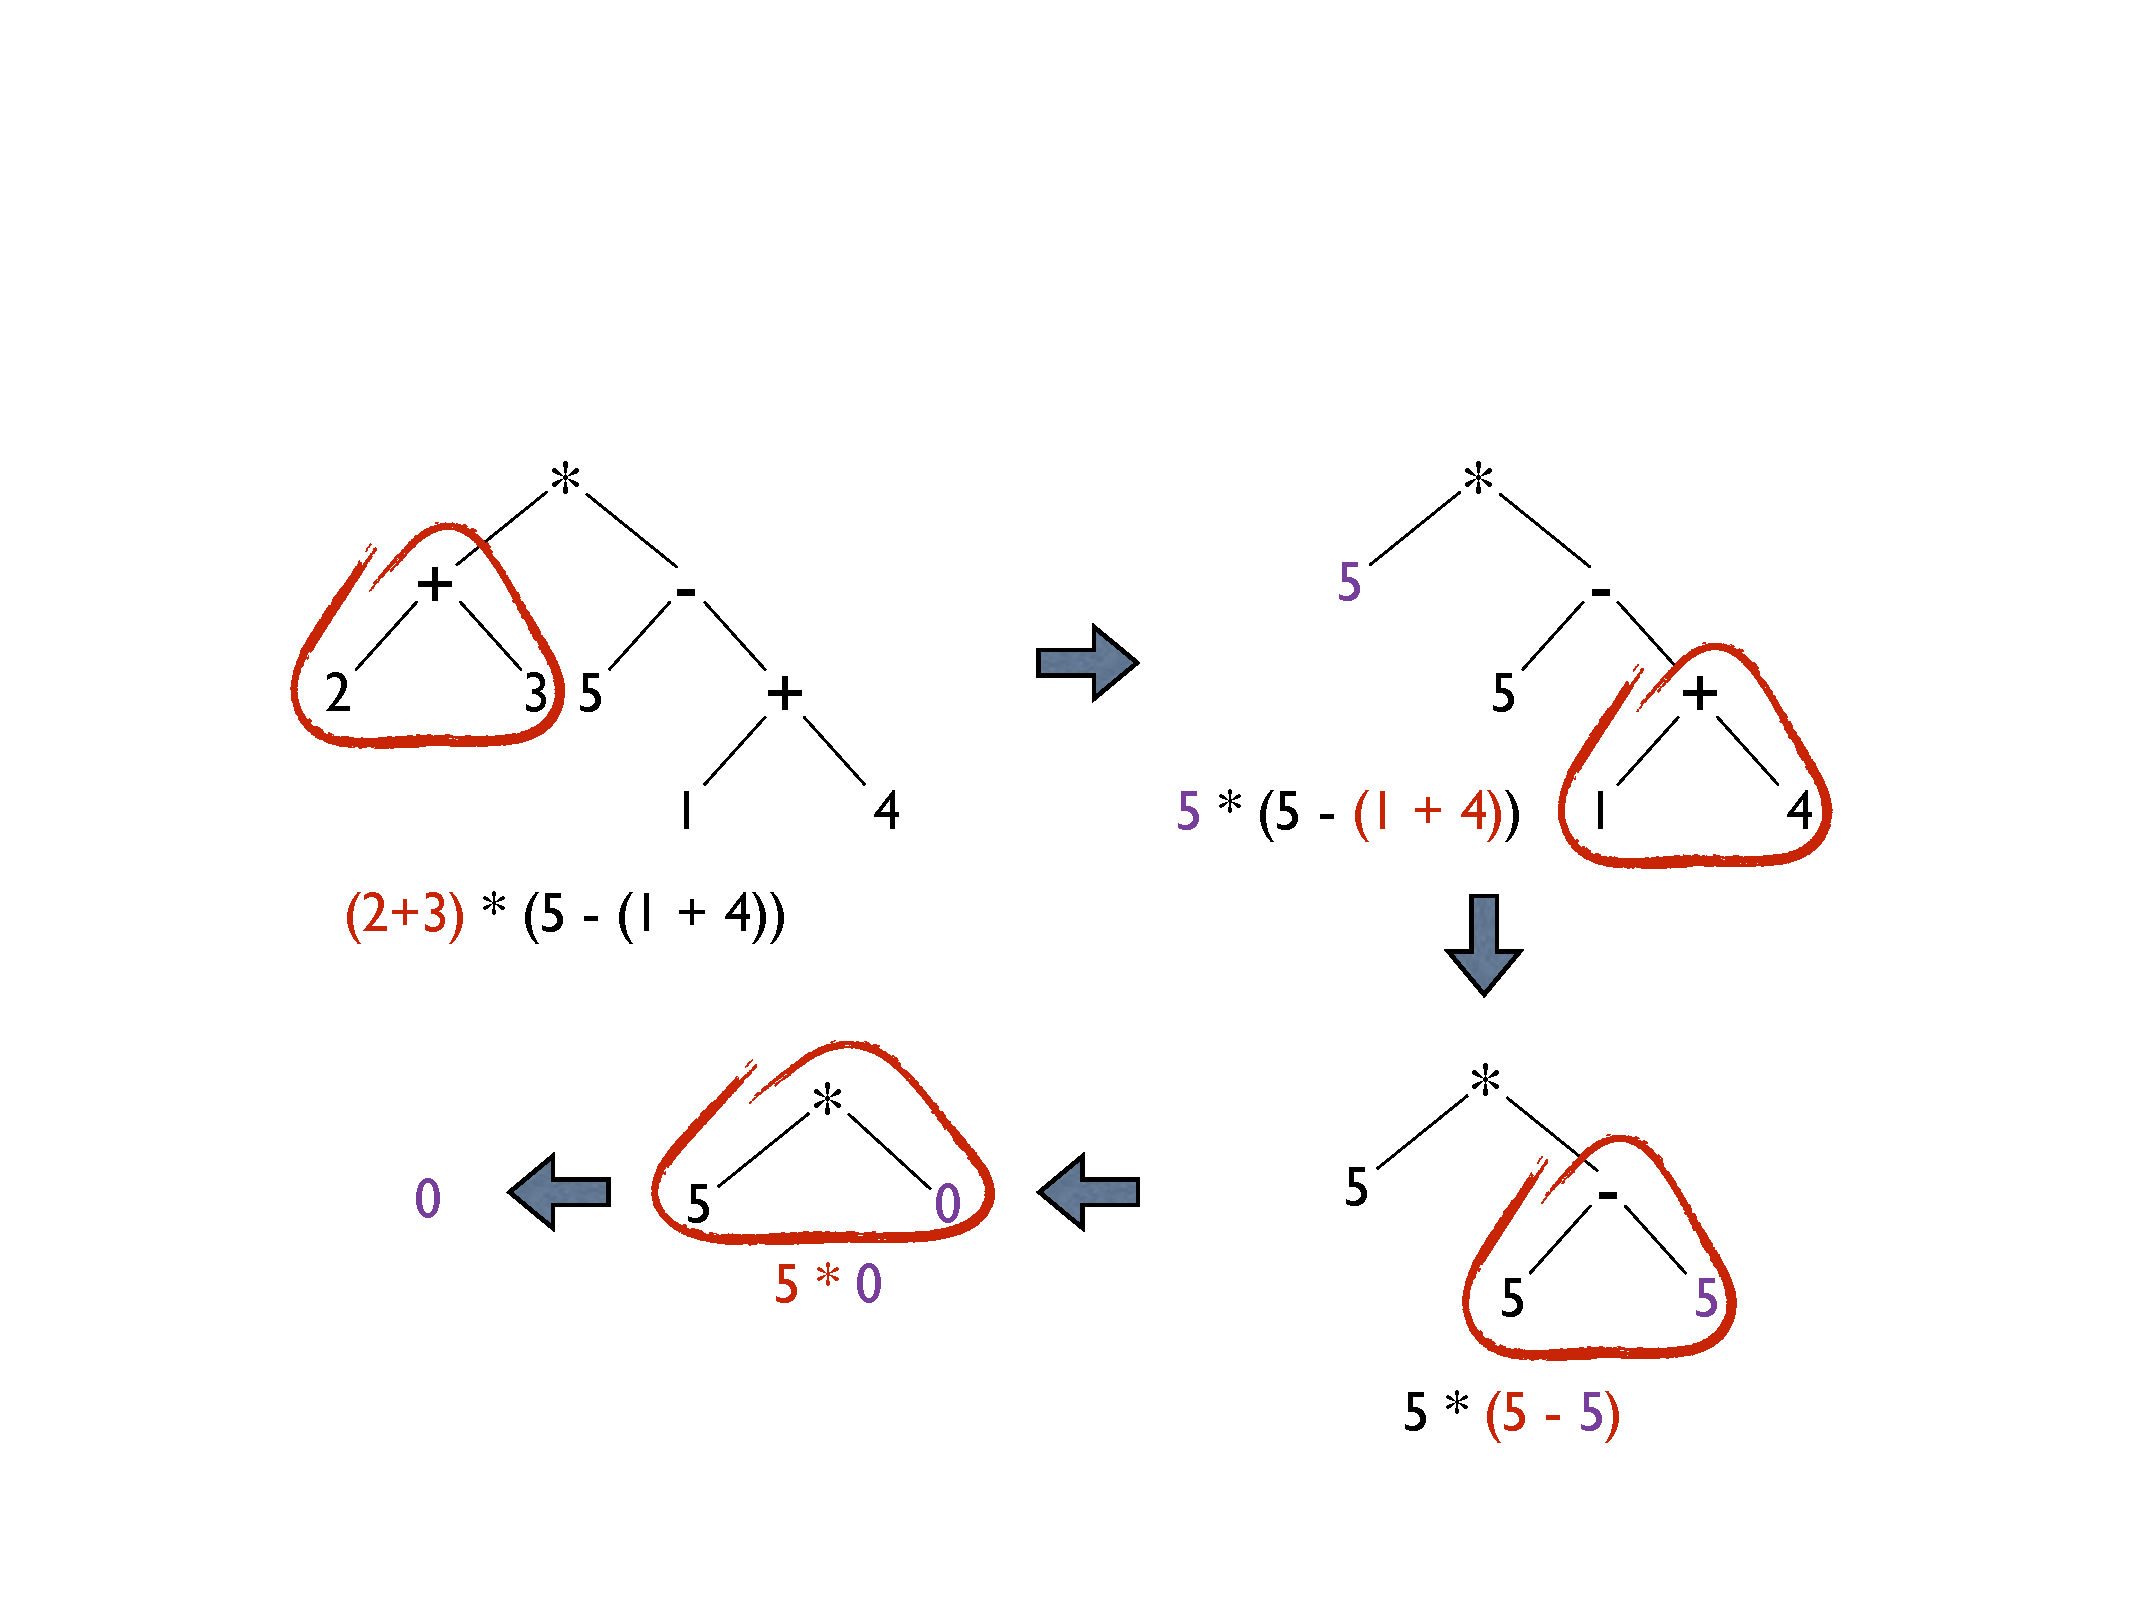
\includegraphics[width=\textwidth]{img/esempio_regole_aritmetiche.pdf}
		\caption{Esempio di applicazione delle regole aritmetiche.}
	\end{figure}
	
	\noindent
	\underline{\textbf{Attenzione!}} Non è possibile eseguire una derivazione di questo tipo:
	\begin{figure}[!htp]
		\centering
		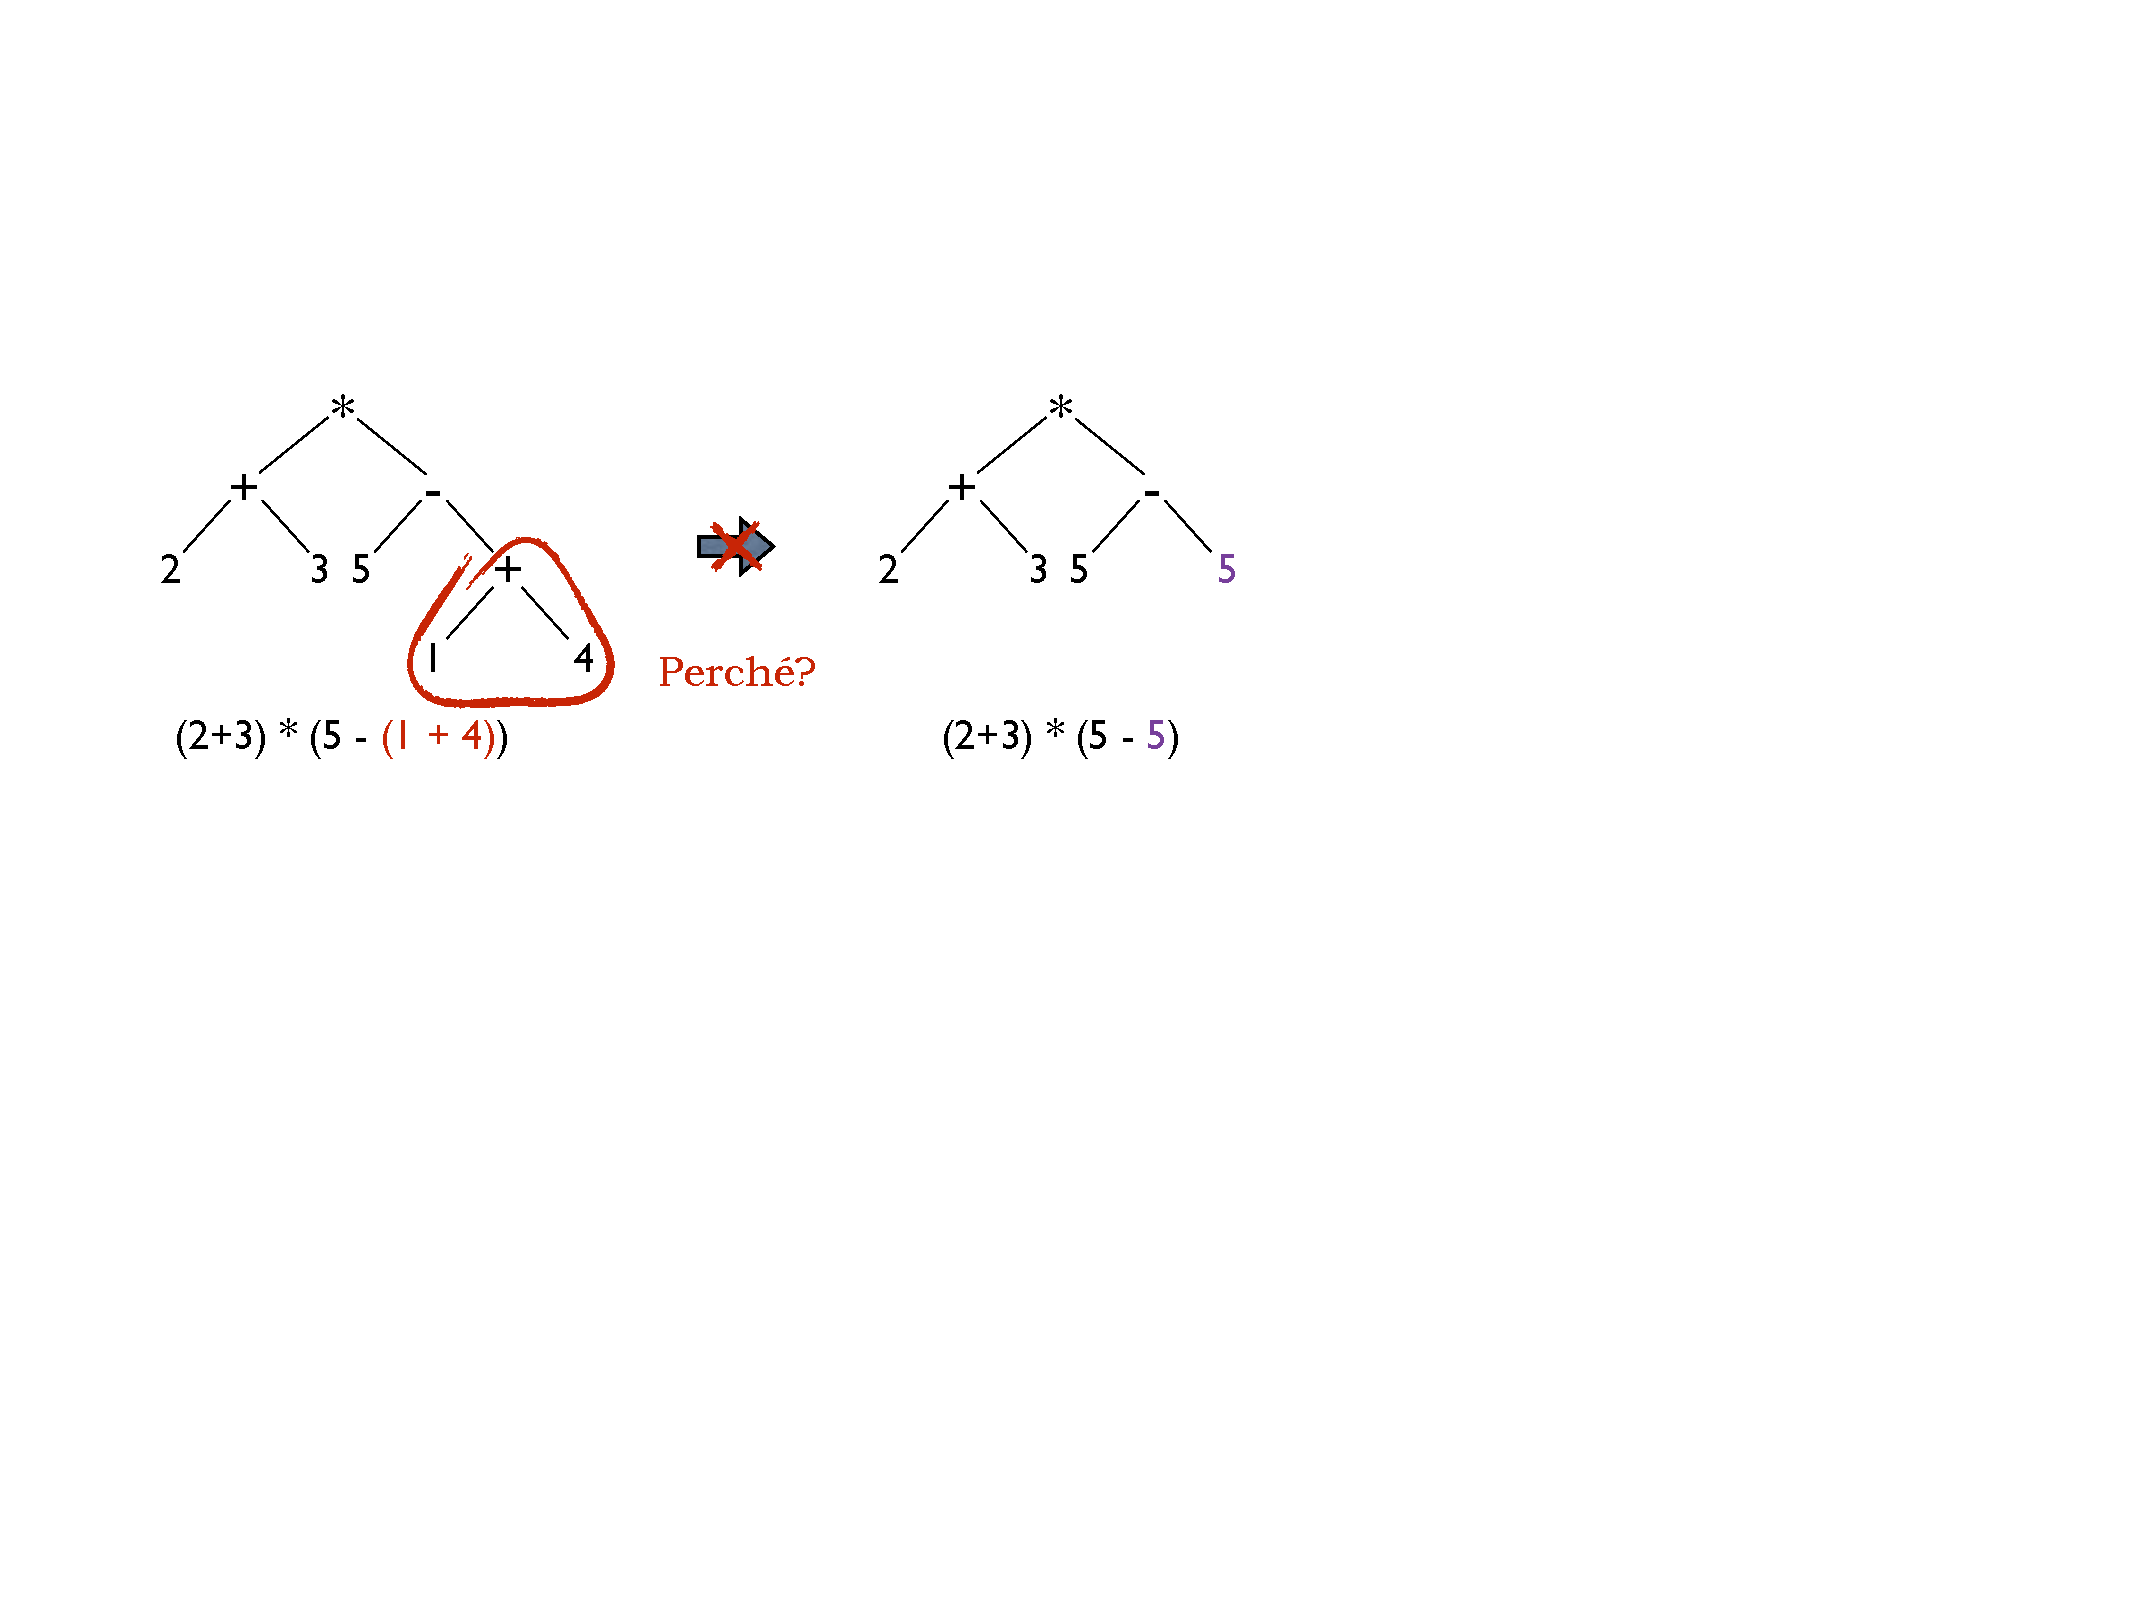
\includegraphics[width=\textwidth]{img/esempio_regole_errato.pdf}
	\end{figure}
	
	\noindent
	Questo perché le regole impongono la valutazione da sinistra verso destra e nella figura viene eseguita una valutazione da destra verso sinistra. Nonostante sia possibile implementare una nuova regola, non avrebbe senso poiché aumenterebbe la possibilità di errore nell'implementazione.
	
	\newpage
	
	\noindent
	Si continua con le regole necessarie per valutare le espressioni booleane (ricordando che \textbf{bop} è il simbolo sintattico di un'operazione e bop è il simbolo dell'operazione nella macchina sottostante):
	\begin{itemize}
		\item È un \underline{assioma} che \textbf{valuta l'espressione sintattica contenente un operatore, nel valore che esso rappresenta}. Ovviamente con valori booleani, i valori coinvolti devono essere tali.
		\begin{figure}[!htp]
			\centering
			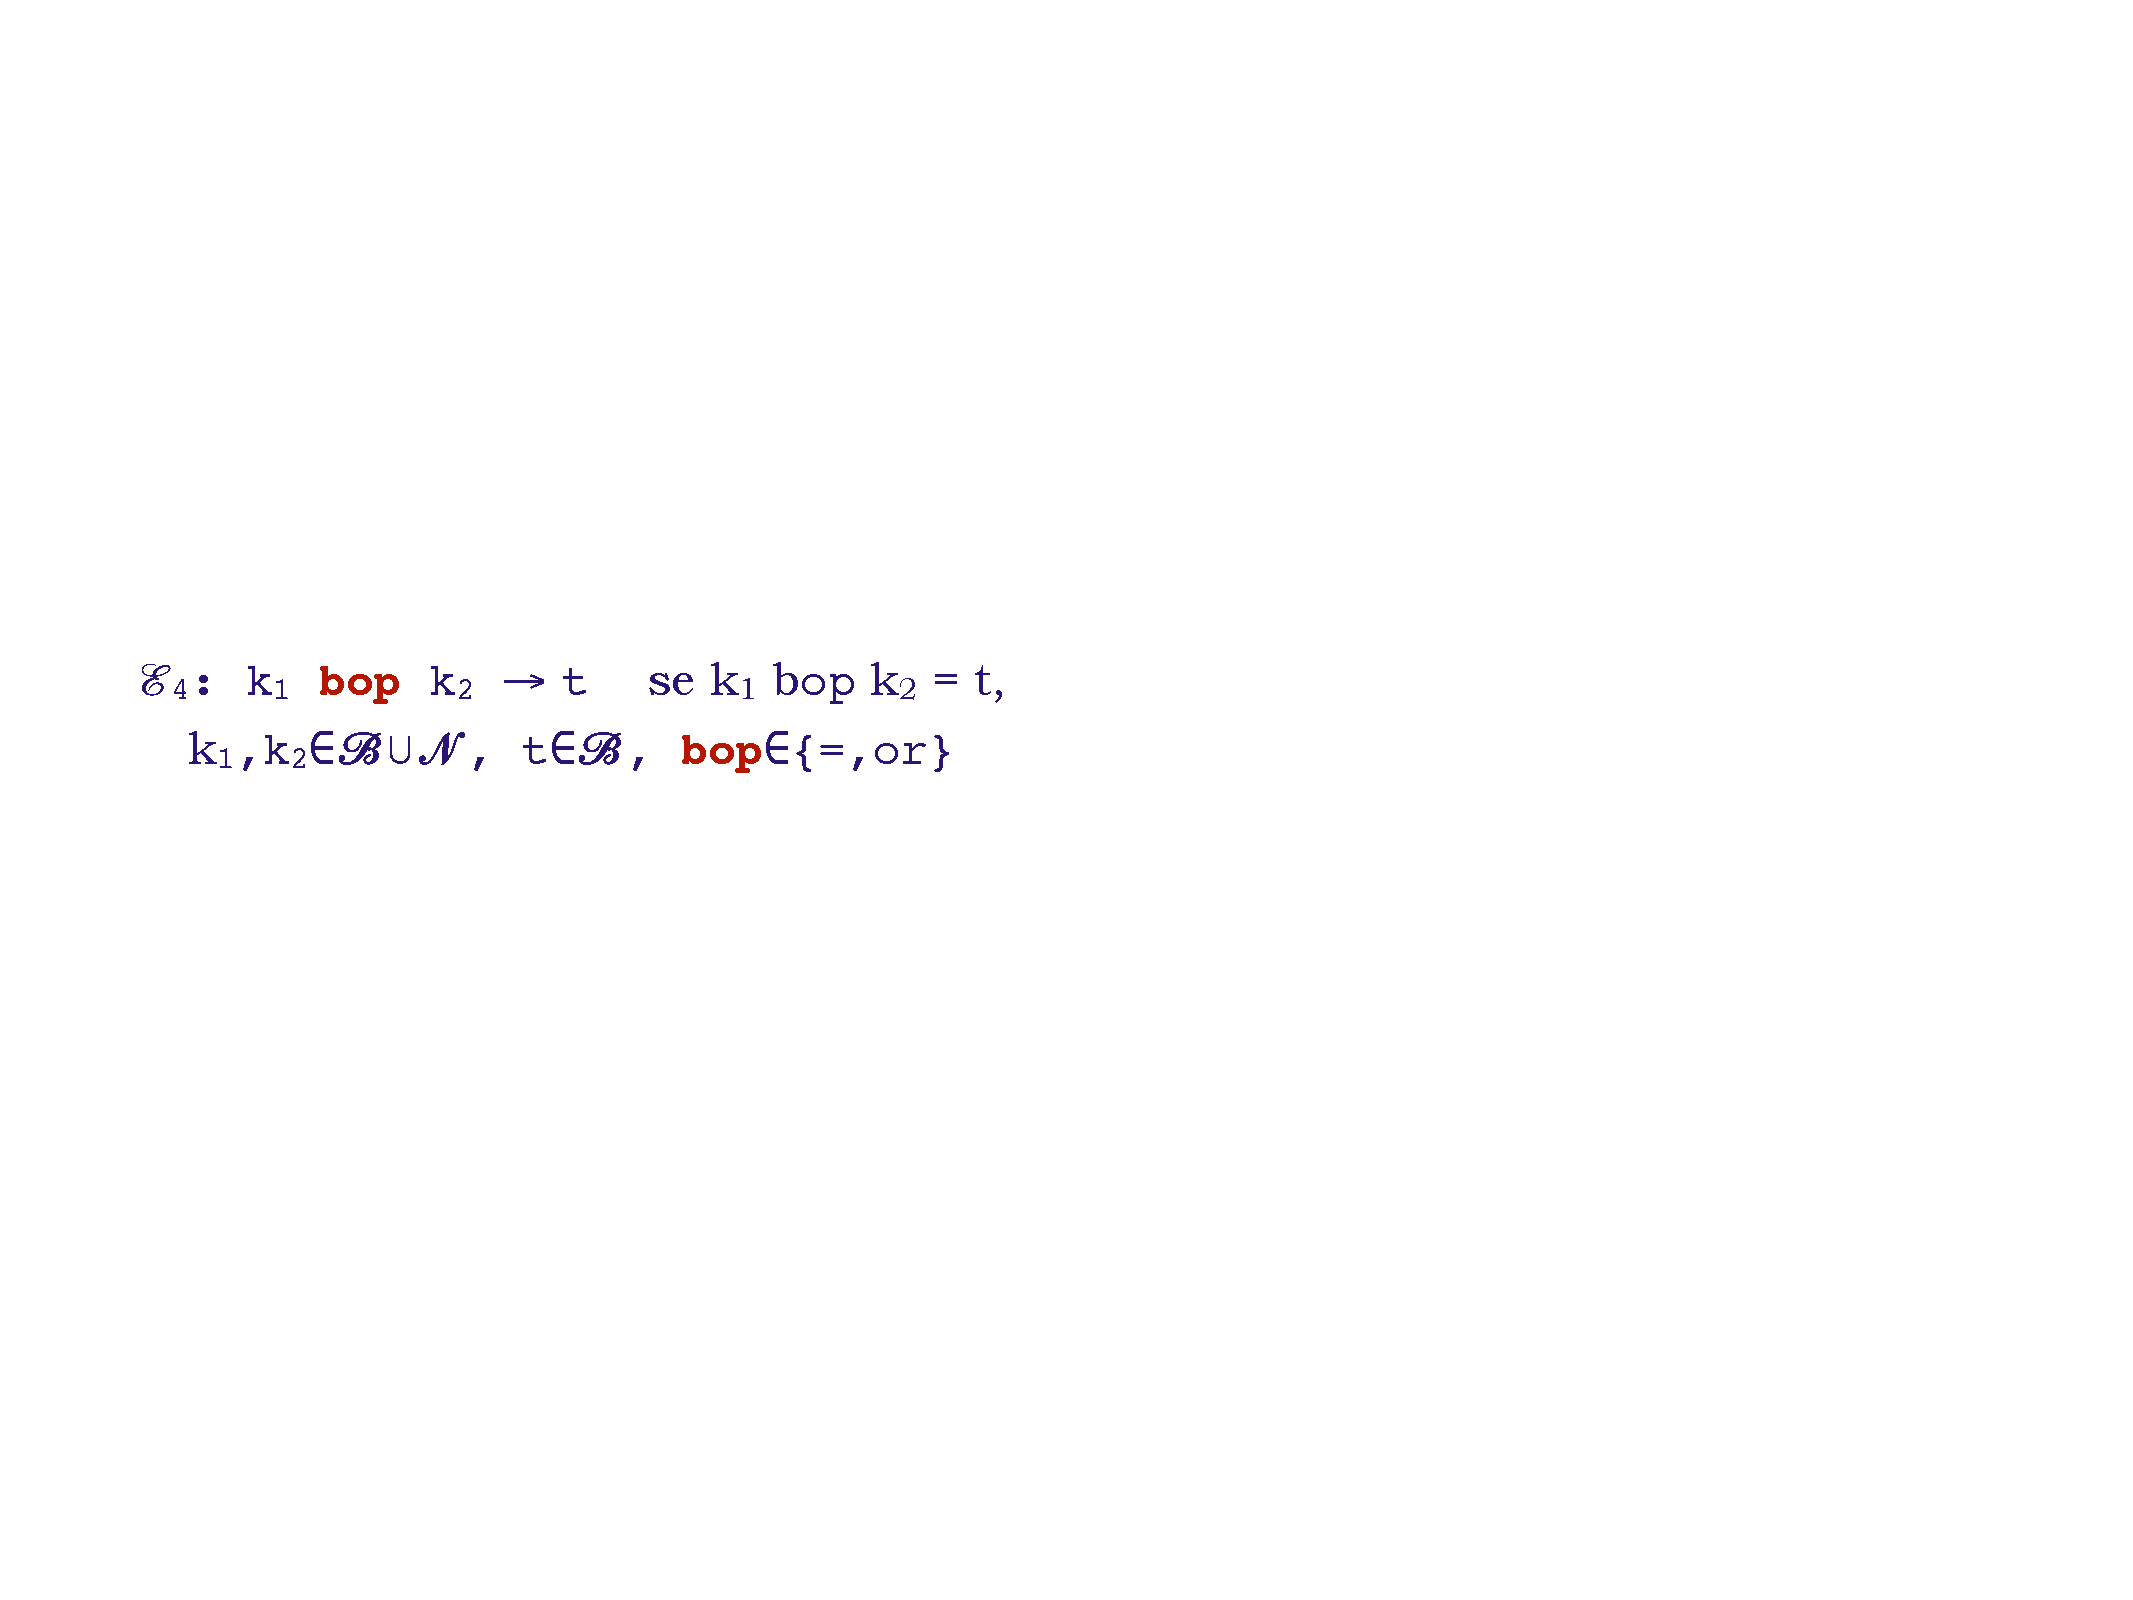
\includegraphics[width=.65\textwidth]{img/regola_transizione-4.pdf}
		\end{figure}
		
		\item Questa regola è una modifica alla precedente poiché \textbf{ammette che l'espressione contenga operatori binari booleani}. L'ordine di valutazione è da sinistra verso destra.
		\begin{figure}[!htp]
			\centering
			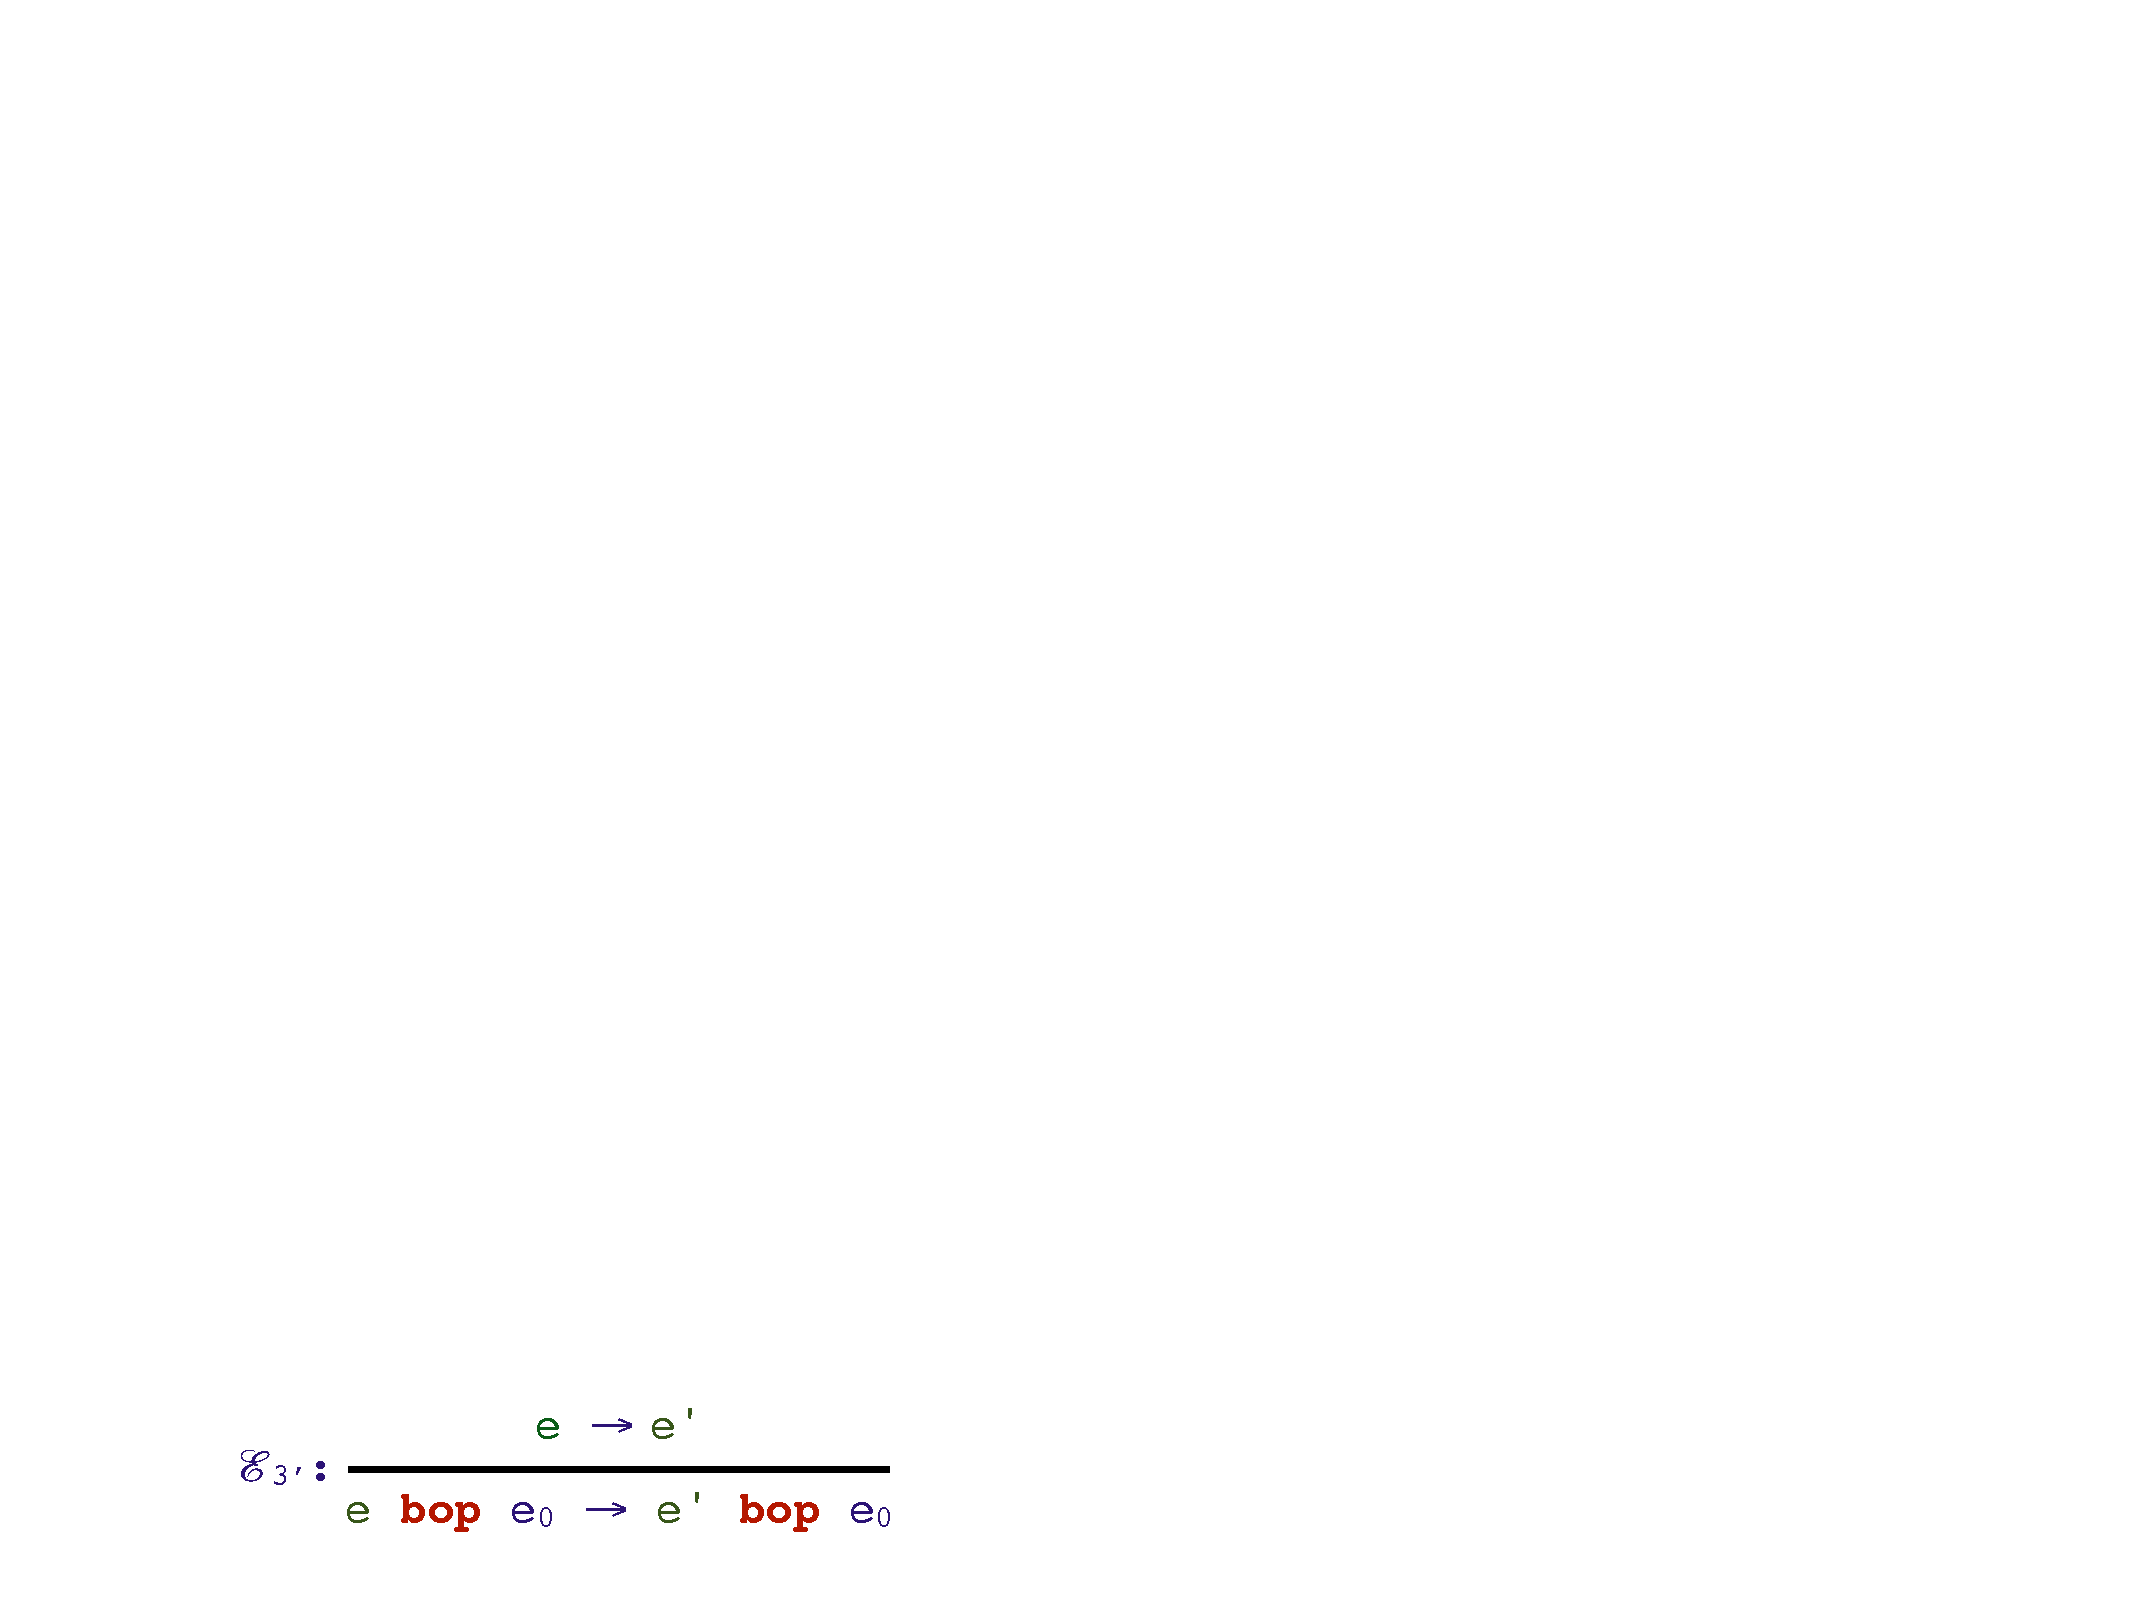
\includegraphics[width=.65\textwidth]{img/regola_transizione-3b.pdf}
		\end{figure}
		
		\item Questa regola stabilisce che nel momento in cui l'\textbf{operando a sinistra è un valore booleano allora è possibile iniziare a valutare l'operando a destra}. Ovviamente, se l'operatore a destra è un valore booleano, allora si ricade nell'assioma $\mathcal{E}_{4}$ ed è possibile restituire il valore finale.
		\begin{figure}[!htp]
			\centering
			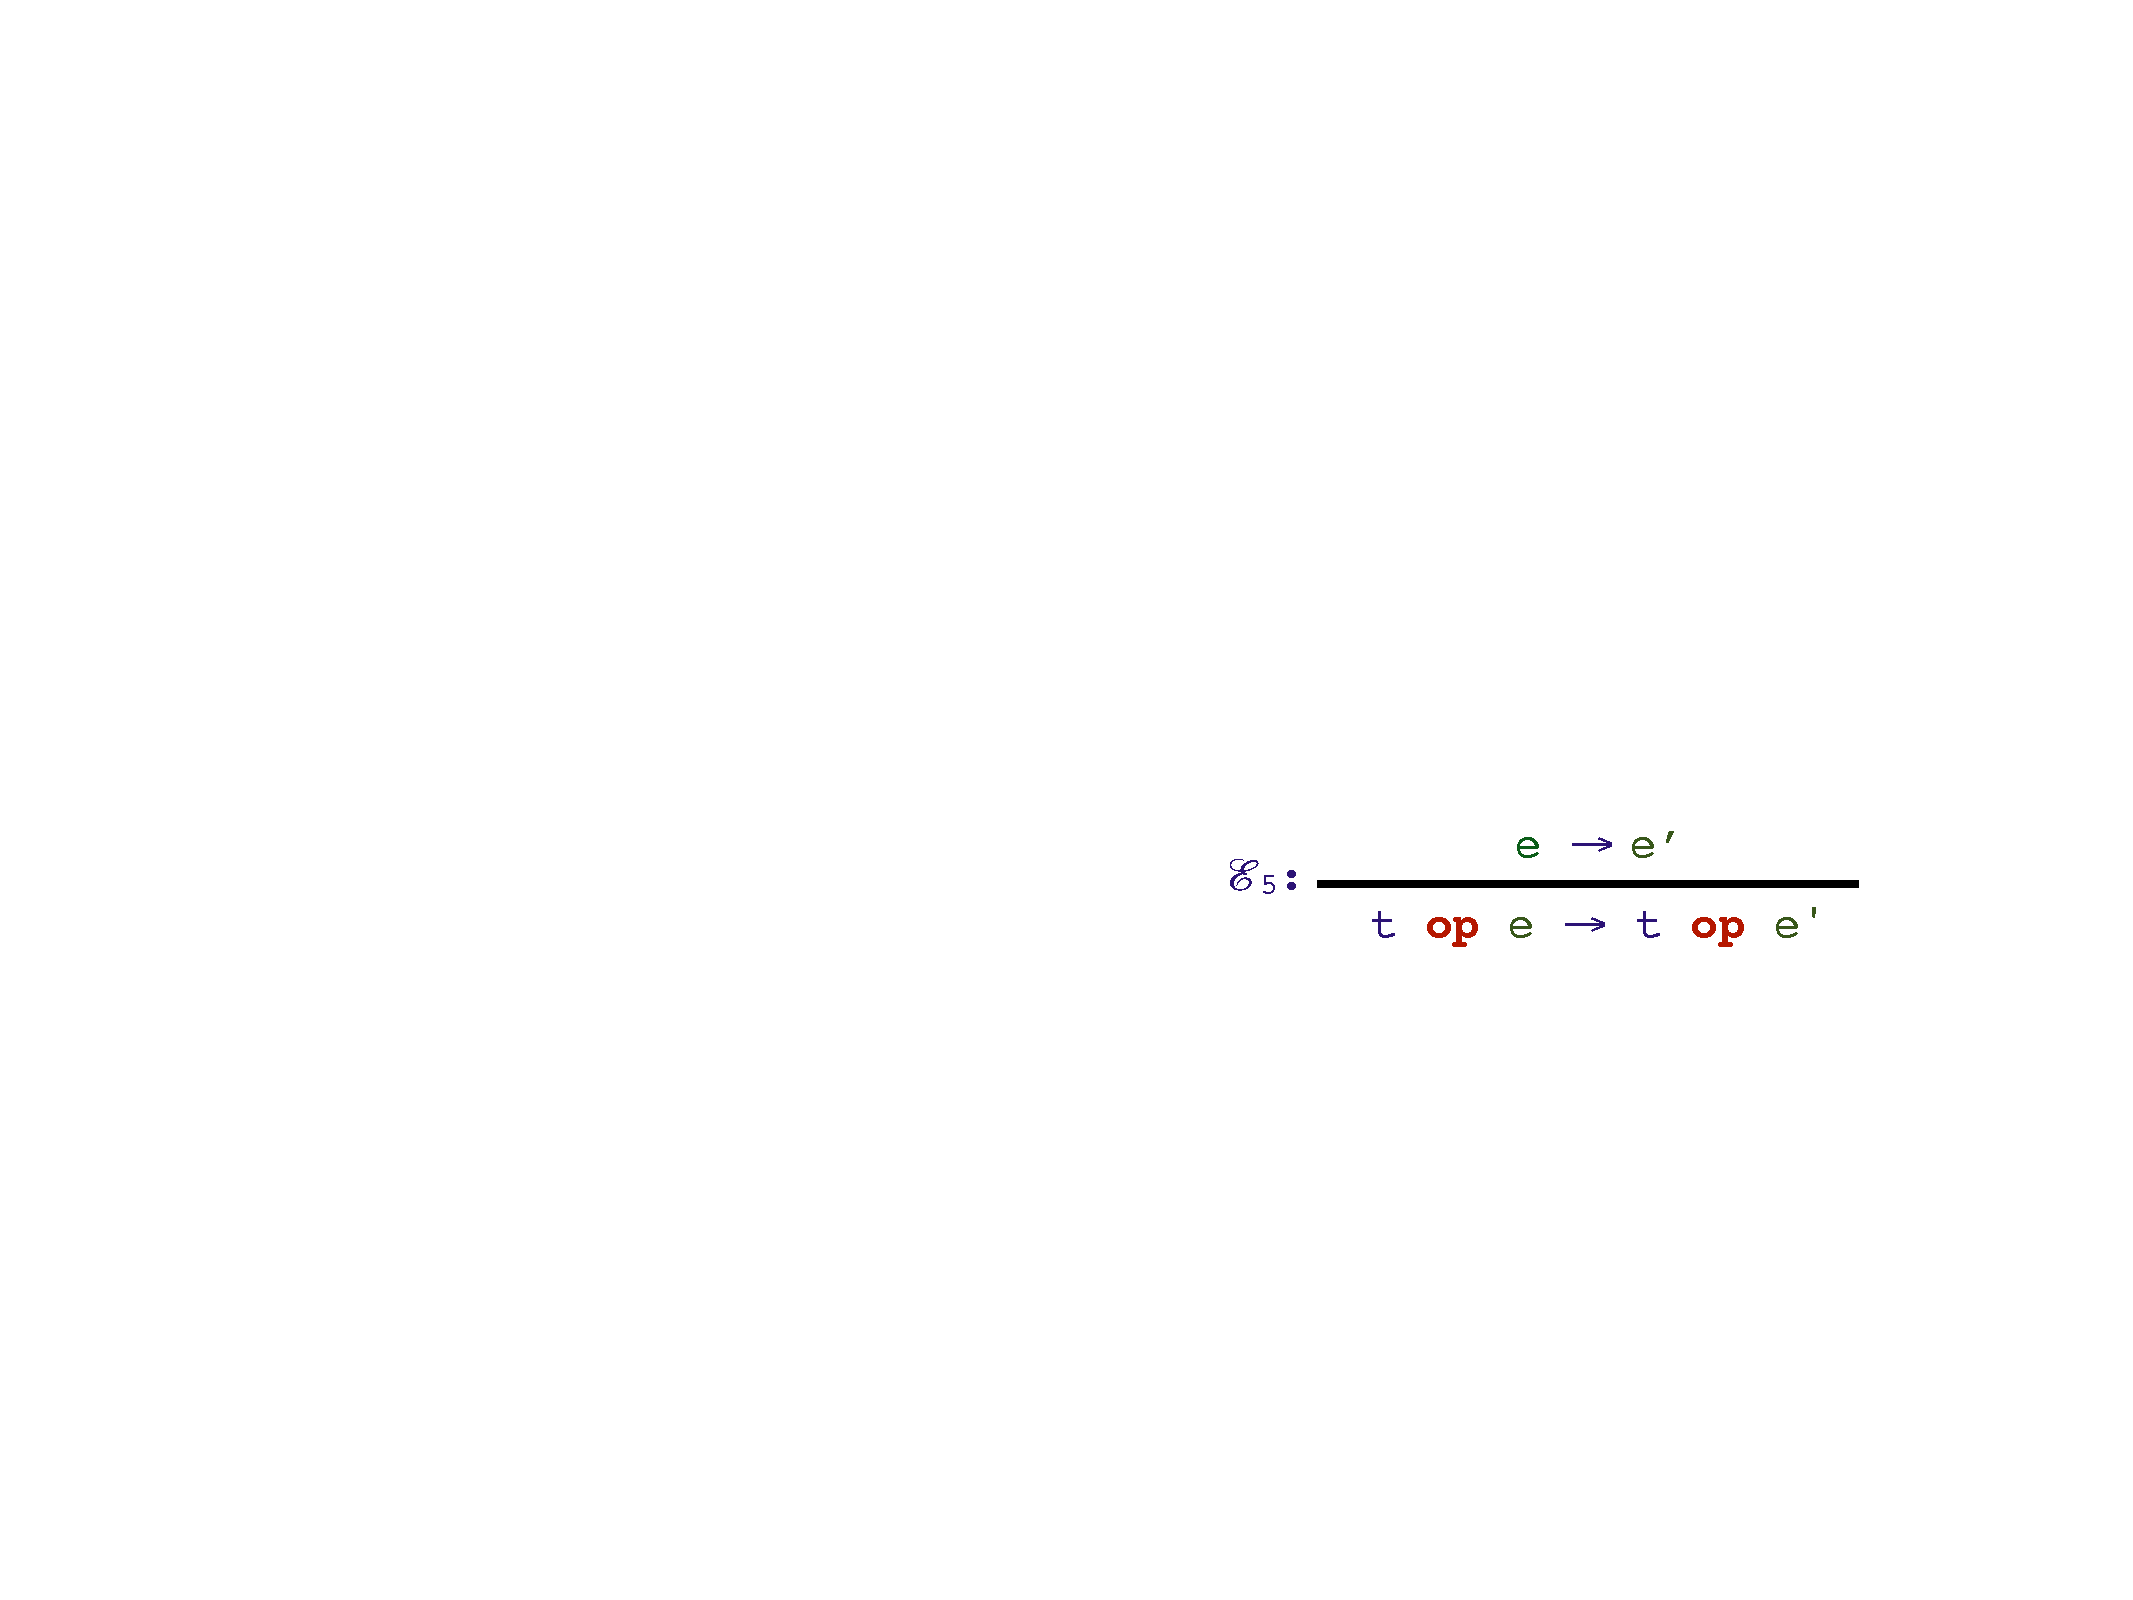
\includegraphics[width=.65\textwidth]{img/regola_transizione-5.pdf}
		\end{figure}
		
		\item Nel caso booleano è necessario aggiungere la \textbf{regola per l'operatore unario}. Quindi si crea l'\underline{assioma} che \textbf{restituisce il valore corrispondente all'applicazione dell'operatore sul valore rappresentato}.
		\begin{figure}[!htp]
			\centering
			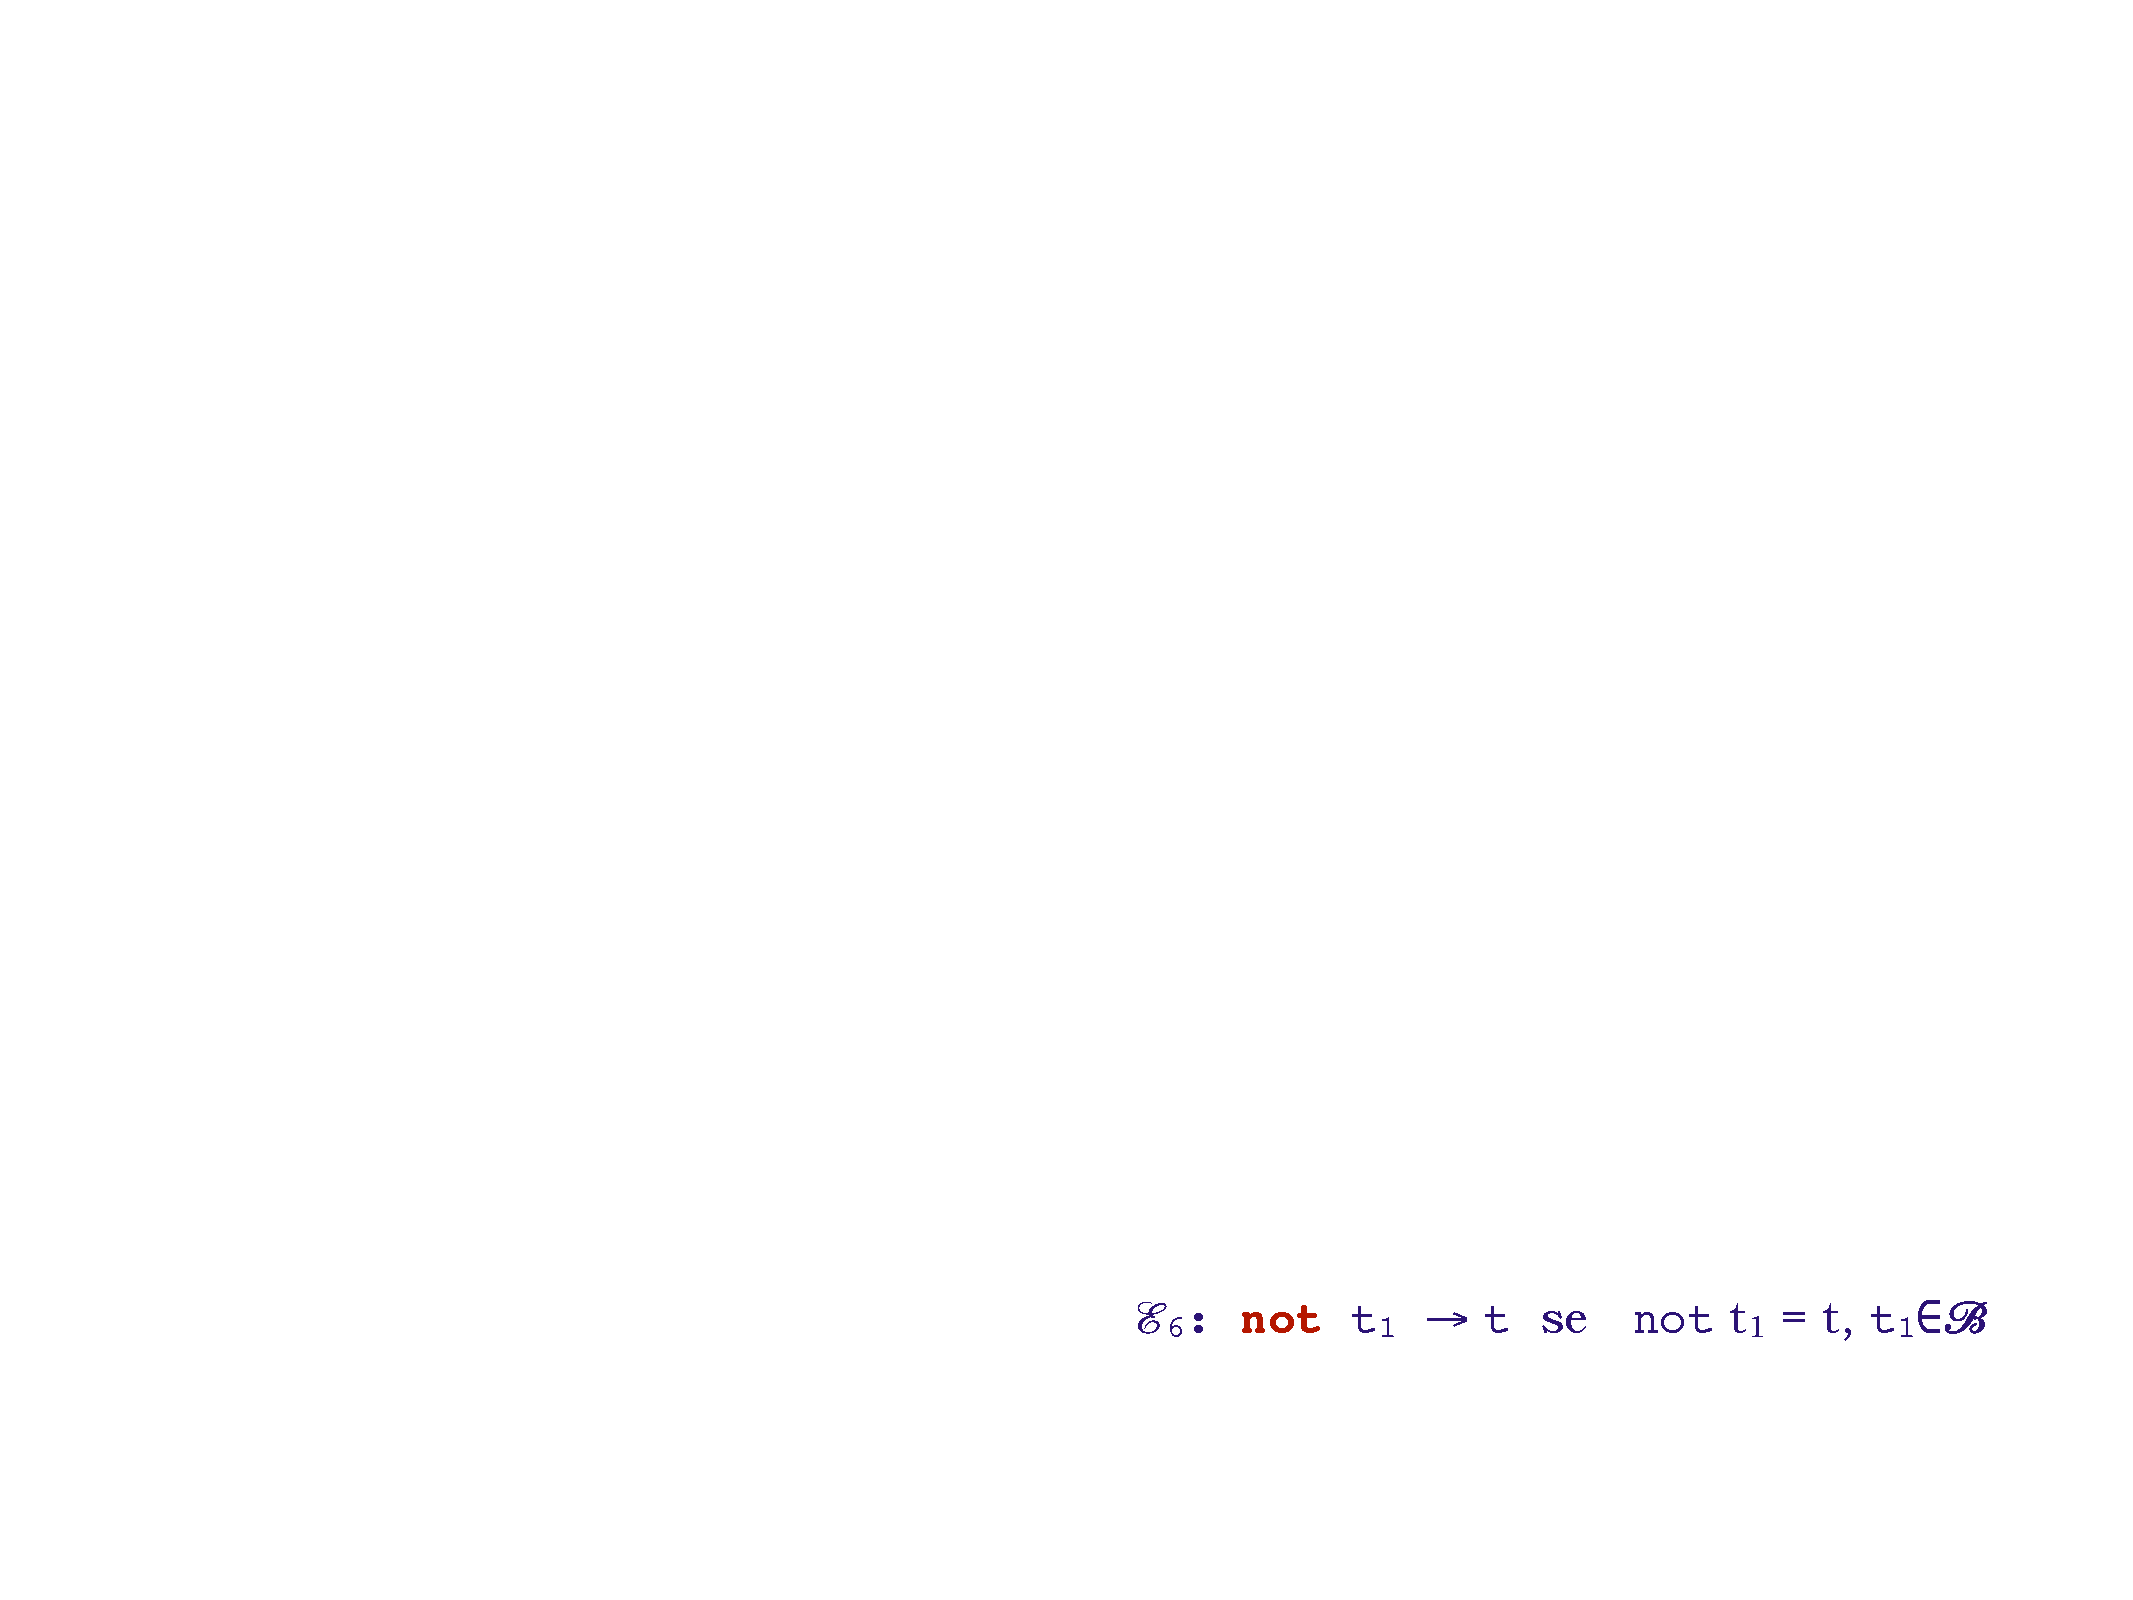
\includegraphics[width=.65\textwidth]{img/regola_transizione-6.pdf}
		\end{figure}
		
		\item Sempre nel caso booleano, si deve creare la \textbf{regola di valutazione}, analoga alle precedenti.
		\begin{figure}[!htp]
			\centering
			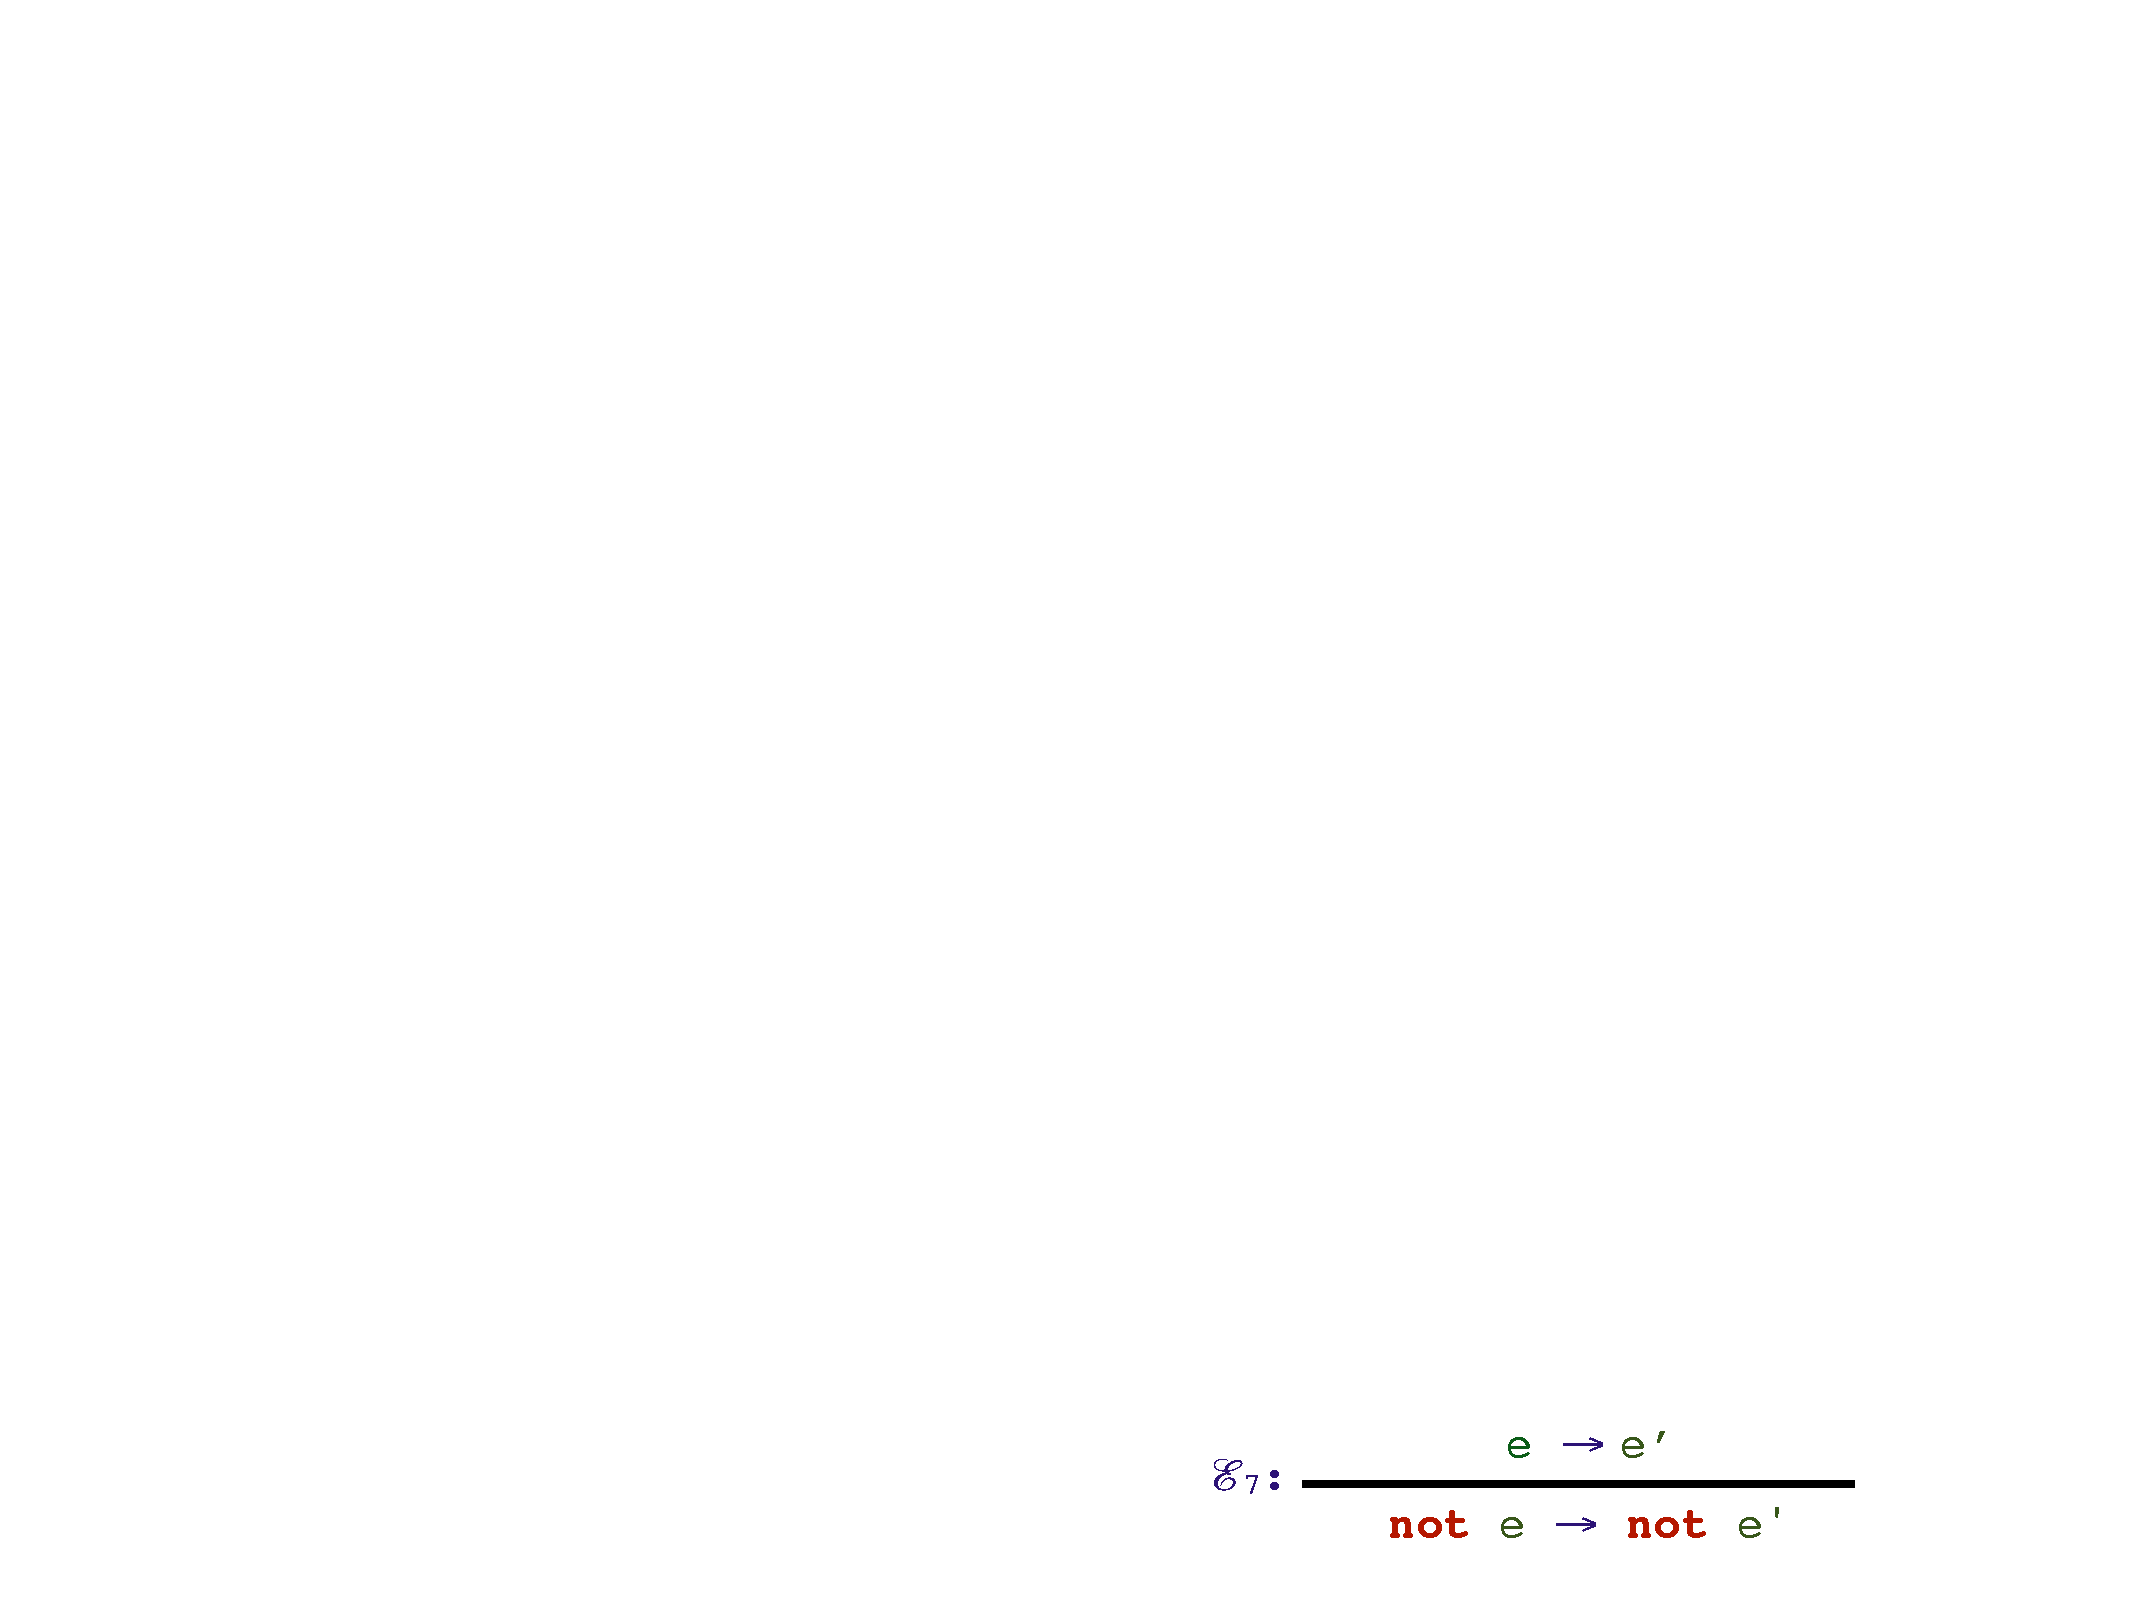
\includegraphics[width=.65\textwidth]{img/regola_transizione-7.pdf}
		\end{figure}
	\end{itemize}\newpage
	
	\subsection{Valutazione ed equivalenza}
	
	\begin{boxdef}
		La \textcolor{Red3}{\textbf{valutazione delle espressioni}} è una \textbf{funzione $Eval: \mathcal{E} \rightarrow \mathbb{N} \cup \mathbb{B}$ che descrive il comportamento dinamico delle espressioni restituendo il valore in cui esse sono valute}:
		\begin{equation*}
			Eval\left(e\right) = k \iff e \rightarrow^* k
		\end{equation*}
	\end{boxdef}\:\newline

	\begin{boxdef}
		L'\textcolor{Red3}{\textbf{equivalenza di espressioni}} è una \textbf{relazione $\equiv \subseteq \mathcal{E} \times \mathcal{E}$ definita come segue}:
		\begin{equation*}
			e_{0} \equiv e_{1} \iff Eval\left(e_{0}\right) = Eval\left(e_{1}\right)
		\end{equation*}
	\end{boxdef}\newpage

	\section{Dichiarazioni}
	
	\subsection{Identificatori}
	
	Gli \textbf{identificatori} sono \textbf{sequenze di caratteri}, che hanno lo \textbf{scopo di denotare} (identificatore appunto) \textbf{qualcos'altro}.\newline
	
	\noindent
	In altre parole, gli \textbf{identificatori sono nomi usati per riferire altri elementi del linguaggio}, come le procedure, \textbf{o della macchina sottostante}, come le colle di memoria, \textbf{durante la computazione}, senza necessariamente conoscerne il valore a priori.\newline
	
	\noindent
	Gli \textbf{identificatori} sono detti \textbf{variabili} quando identificano celle di memoria.\newline
	
	\noindent
	I \textbf{nomi} sono fondamentali per gli identificatori perché sono \textbf{facili da ricordare} e consentono di effettuare un processo di \textbf{astrazione}. Inoltre, è importante sottolineare il fatto che un identificatore ed un oggetto denotato \underline{non} sono la stessa cosa:
	\begin{itemize}
		\item Un identificatore può denotare più elementi;
		\item Un elemento può essere denotato da più identificatori diversi (\emph{aliasing})
	\end{itemize}
	Un \textcolor{Green4}{\textbf{esempio}} è il seguente codice:
	\begin{lstlisting}[language=C]
const pi = 3.14;
int x;
void f(){...};\end{lstlisting}
	Gli oggetti denotati sono una costante, una variabile e una procedura:
	\begin{itemize}
		\item \textsf{3.14} è una costante;
		\item \textsf{x} è una variabile;
		\item \textsf{\{...\}} è una procedura
	\end{itemize}
	Mentre \textsf{pi, x, f} sono nomi.\newline
	
	\noindent
	In definitiva, gli identificatori non possono essere stringhe di caratteri qualunque, ma devono seguire delle regole così che il \emph{parser} del linguaggio li possa riconoscere come tali.\newline
	
	\noindent
	\begin{boxdef}
		Gli \textcolor{Red3}{\textbf{identificatori}} sono una \textbf{sequenza di caratteri usata per rappresentare o \underline{denotare} un altro oggetto}.
	\end{boxdef}\newpage
	
	\subsection{Bindings}
	
	\subsubsection{Legami}
	
	\begin{boxdef}
		Il \textcolor{Red3}{\textbf{\emph{binding occurrences}}} o in italiano la \textcolor{Red3}{\textbf{creazione \emph{binding}}} è il momento in cui viene \textbf{\underline{definito} il nome (identificatore) e il suo significato (denotazione)}.
	\end{boxdef}

	\noindent
	In \textbf{matematica} questo accade ogni volta che viene posto un problema enunciando (e.g.) \dquotes{sia $x$ ...}. Viene creato un \emph{binding} \textbf{tra il significato dichiarato e il nome che verrà poi utilizzato nella specifica del problema}. In \textbf{logica} i \emph{binding} sono creati dai quantificatori (universali o esistenziali).\newline
	
	\noindent
	In \textbf{programmazione} i \emph{binding} sono creati dalle dichiarazioni. Successivamente, il nome può essere correttamente utilizzato per riferirsi/rappresentare il suo significato.\newline
	
	\noindent
	\begin{boxdef}
		L'\textcolor{Red3}{\textbf{\emph{applied occurrences}}} o in italiano l'\textcolor{Red3}{\textbf{applicazione \emph{binding}}} è il momento in cui viene \textbf{\underline{utilizzato} il nome (identificatore) per \underline{accedere} al suo significato (denotazione)}.
	\end{boxdef}

	\noindent
	In programmazione, come in matematica, non è sempre necessario creare i \emph{binding} prima del loro utilizzo, dipende dal linguaggio di programmazione.\newline
	
	\noindent
	Un \textcolor{Green4}{\textbf{esempio}} di creazione e applicazione:
	\begin{gather*}
		\displaystyle\sum_{i=1}^{n}\sum_{j=1}^{m}a_{ij} \cdots b_{jk} \\
		\downarrow \\
		\displaystyle\underbrace{\sum_{i=1}^{n}\sum_{j=1}^{m}}_{\text{\emph{Binding occurrences i,j}}} \overbrace{a_{ij} \cdots b_{jk}}^{\text{\emph{Applied occurrences i,j}}}
	\end{gather*}
	La $i$ e $j$ sotto il simbolo di sommatoria sulla sinistra indicano la creazione del \emph{binding} e la $i,j$ a pedice dei simboli $a$ e $b$ sulla destra indicano l'applicazione del \emph{binding}.\newpage
	
	\subsubsection{Scope}
	
	Esistono anche le occorrenze libere che sono simili a quelle applicate con l'unica differenza che riguarda il raggio di azione (\emph{scope}) di un'occorrenza di definizione.\newline
	
	\noindent
	\begin{boxdef}
		Le \textcolor{Red3}{\textbf{\emph{free occurrences}}} o in italiano le \textcolor{Red3}{\textbf{occorrenze libere}} (non legate) è il momento in cui viene \textbf{\underline{utilizzato} un nome (identificatore) il cui significato (denotazione) non è stato definito}.
	\end{boxdef}\:\newline

	\noindent
	\begin{boxdef}
		Lo \textcolor{Red3}{\textbf{\emph{scope} di un \emph{binding}}} o in italiano il \textcolor{Red3}{\textbf{raggio d'azione di una definizione}} è la \textbf{definizione di spazio in cui è possibile utilizzare un nome per rappresentare il significato associato da un \emph{binding}}.
	\end{boxdef}\:\newline

	\noindent
	Un \textcolor{Green4}{\textbf{esempio}} di creazione e applicazione:
	\begin{gather*}
		\displaystyle\sum_{i=1}^{n}\sum_{j=1}^{m}a_{ij} \cdots b_{jk} \\
		\downarrow \\
		\displaystyle\underbrace{\sum_{i=1}^{n}\overbrace{\sum_{j=1}^{m} a_{ij} \cdots b_{jk}}^{\text{Scope di \emph{j}}}}_{\text{Scope di \emph{i}}}
	\end{gather*}
	La $n$, la $m$ e la $k$ sopra il simbolo di sommatoria sulla sinistra e al pedice della $b$, indicano le occorrenze libere, cioè non legate. Invece, lo \emph{scope} di $j$ si concentra sulla sommatoria più innestata, mentre lo \emph{scope} di $i$ sulla sommatoria più esterna.\newpage
	
	
	\subsubsection{Bindings nei linguaggi di programmazione}
	
	Si riportano le definizioni già date ma con una veste diversa (non so il motivo di questa scelta, ma sulle slide è così...).\newline
	
	\noindent
	\begin{boxdef}
		\textcolor{Red3}{\textbf{Definizione - \emph{Binding occurrence}:}} un identificatore in posizione di definizione quando si \emph{(ri)definisce il significato} dell'identificatore.
	\end{boxdef}\:\newline

	\noindent
	\begin{boxdef}
		\textcolor{Red3}{\textbf{Uso - \emph{Applied occurrence}:}} un identificatore in posizione di uso quando si \emph{riferisce/denota il significato} definito da una definizione.
	\end{boxdef}\:\newline
	
	\noindent
	\begin{boxdef}
		\textcolor{Red3}{\textbf{Libera - \emph{Free occurrence}:}} un identificatore in posizione libera se il suo uso non è nel \emph{raggio di azione (scope)} di una definizione.
	\end{boxdef}\newpage
	
	
	\subsubsection{Tipi di bindings nei linguaggi di programmazione}
	
	A seconda dell'oggetto denotato, il \emph{binding} creato è di tipo diverso:
	\begin{itemize}
		\item \textbf{Nome-Valore}: quando il \textbf{legame non può cambiare}, allora viene legato il nome ad un valore.
		
		\item \textbf{Nome-Locazione}: \textbf{legame non modificabile}
		
		\item \textbf{Locazione-Valore} \textbf{legame modificabile}
	\end{itemize}
	Tutti i \textbf{legami} sono \textbf{immutabili} ed esistono due tipi di \emph{binding}:
	\begin{itemize}
		\item \textbf{Binding \emph{statico}} è tale \textbf{se occorre per la prima volta prima dell'esecuzione e rimane invariato durante tutta l'esecuzione del programma}.\newline
		Per \textcolor{Green4}{\textbf{esempio}}, i tipi delle variabili in linguaggi fortemente tipati.
		
		\item \textbf{Binding \emph{dinamico}} è tale \textbf{se occorre durante l'esecuzione e può variare}.\newline
		Per \textcolor{Green4}{\textbf{esempio}}, i \textbf{legami tra locazioni/celle di memoria e valori contenuti nelle locazioni}.
	\end{itemize}\newpage
	
	\subsubsection{Tempi}
	
	Esistono due \textbf{tipi di \underline{creazione} dei \emph{binding}}:
	\begin{itemize}
		\item \textcolor{Red3}{\textbf{Tempo di compilazione}} (\emph{Early binding}). Ogni nome viene risolto a tempo di compilazione, quindi è presente un'\textbf{allocazione statica della memoria} con indirizzi assoluti.
		\begin{itemize}
			\item \textcolor{Green4}{\textbf{Pro:}} esecuzione estremamente veloce
			
			\item \textcolor{Red3}{\textbf{Contro:}} programmazione poco flessibile
			
			\item \textbf{Esempi di linguaggi:}  Fortran\footnote{Un interessante articolo sul perché Fortran viene ancora utilizzato: \href{https://www.matecdev.com/posts/why-fortran-still-used.html}{link}}, Cobol.
		\end{itemize}
		
		\item \textcolor{Red3}{\textbf{Tempo di esecuzione}} (\emph{Late binding}). Tutto avviene a tempo di esecuzione, quindi la \textbf{memoria è allocata dinamicamente}, tutti i \emph{binding} vengono creati dinamicamente con indirizzi non assoluti.
		\begin{itemize}
			\item \textcolor{Green4}{\textbf{Pro:}} programmazione più flessibile
			
			\item \textcolor{Red3}{\textbf{Contro:}} esecuzione più lenta
			
			\item \textbf{Esempi di linguaggi:} Snobol4, Lisp, APL.
		\end{itemize}
	\end{itemize}
	Invece, qui di seguito vengono elencati degli \textbf{esempi di tempi di bindings}:
	\begin{itemize}
		\item Tempo di \textbf{progettazione}, \emph{bindings} di operatori ($+,-,...$) ai simboli;
		
		\item Tempo di \textbf{implementazione di linguaggi}, \emph{binding} del tipo floating point con la propria rappresentazione;
		
		\item Tempo di \textbf{compilazione}, \emph{binding} delle variabili con i loro tipo, come in C o Java;
		
		\item Tempo di \textbf{caricamento}, \emph{binding} variabili \textsf{static} alla cella di memoria;
		
		\item Tempo di \textbf{esecuzione}, \emph{binding} variabili non statiche con la cella di memoria.
	\end{itemize}
	Quindi, dovrebbe essere chiara la \textbf{fondamentale importanza dei \emph{bindings}}: un identificatore/nome non ha significato se non è legato a qualcosa, se non è coinvolto almeno in un \emph{binding}. Per \textcolor{Green4}{\textbf{esempio}}, un'espressione non ha significato/valore se contiene nomi non legati a nulla.\newpage
	
	
	\subsection{Semantica: Identificatori, ambienti e dichiarazioni}
	
	Nei linguaggi di programmazione, per riferire \textbf{valori generati dalle espressioni}, viene utilizzato il concetto di \textcolor{Red3}{\textbf{identificatore}}. Esso è un \textbf{nome che viene associato all'oggetto da identificare/riferire}.\newline
	
	\noindent
	Per riferire i valori (oggetti denotabili) associati agli identificatori, viene utilizzato il concetto di \textcolor{Red3}{\textbf{ambiente}}, il quale è definito come l'insieme di legami (\emph{bindings}) tra identificatori e oggetti \textbf{denotabili}, ovvero tutti quegli oggetti del linguaggio che sono riferibili mediante un identificatore.
	
	In altre parole, l'ambiente è la componente della macchina astratta che per ogni nome introdotto dal programmatore, e per ogni punto di programma, consente di determinare quale sia l'associazione corretta.\newline
	
	\noindent
	Infine, la \textbf{dichiarazione} implementa la creazione dei legami.\newline
	
	\noindent
	\begin{boxdef}
		L'\textcolor{Red3}{\textbf{ambiente}} è l'\textbf{insieme delle associazioni fra nomi e oggetti denotabili esistenti a \emph{run-time} in uno specifico punto del programma ed in uno specifico momento dell'esecuzione}.
	\end{boxdef}
	\begin{boxdef}
		La \textcolor{Red3}{\textbf{dichiarazione}} è il \textbf{meccanismo (implicito o esplicito) col quale si crea un'associazione nell'ambiente}.
	\end{boxdef}\newpage

	
	\subsubsection{Termini chiusi e ground}
	
	\begin{boxdef}
		\textbf{In un linguaggio (con identificatori),un \textcolor{Red3}{termine} in cui non ci sono identificatori liberi è detto \textcolor{Red3}{chiuso}.}
	\end{boxdef}
	
	\noindent
	Il significato delle frasi chiuse è quello di \textbf{dare significato alla frase senza richiedere un ambiente esterno}. In termini tecnici, significa che un \textbf{programma}, ad esempio, \textbf{non ha identificatori liberi e quindi può essere eseguito a partire da un ambiente vuoto}, in quanto non ci sono identificatori che richiedono un significato all'esterno.\newline

	\noindent
	Per \textcolor{Green4}{\textbf{esempio}}, non è possibile dare significato ad $a+b+c+x$ se non viene dato un significato ad $a,b,c,x$. È dunque necessario di assunzioni sull'ambiente, le quali riguardano l'insieme di \emph{binding} per gli identificatori, ovvero uguaglianze del tipo $nome = entità$.\newline
	
	\noindent
	Quindi, un \textbf{programma è una \textcolor{Red3}{frase chiusa} se ogni occorrenza d'uso è preceduta da un'occorrenza di definizione che stabilisce il significato dell'identificatore}.\newline
	
	\noindent
	\begin{boxdef}
		\textbf{In un linguaggio (con identificatori), un \textcolor{Red3}{termine} in cui non ci sono identificatori è detto \textcolor{Red3}{\emph{ground}}.}
	\end{boxdef}
	
	\noindent
	Data l'assenza di identificatori, il \textbf{termine \emph{ground}} non richiede neanche un ambiente.\newpage
	
	\subsubsection{Ambienti nei linguaggi imperativi}
	
	Nel \textbf{linguaggio imperativo} si considerano solo \textbf{interi e booleani} (per semplicità), quindi gli unici oggetti denotabili sono:
	\begin{equation*}
		\begin{array}{rl}
			\mathcal{N} = \text{ Insieme di numerali nella macchina sottostante:} & \textsf{m,n,p} \\
			\mathcal{B} = \left\{\textsf{true}, \textsf{false}\right\}: & \textsf{t}
		\end{array}
	\end{equation*}
	\begin{boxdef}
		Un \textcolor{Red3}{\textbf{ambiente dinamico}} è un elemento dello spazio di funzioni tale che:
		\begin{equation*}
			Env = \cup_{V \subseteq_{f} Id} Env_{V}
		\end{equation*}
		In cui:
		\begin{equation*}
			Env_{V}: V \rightarrow DVal \hspace{2em} \cup\left\{\bot\right\} \text{ ha metavariabile }\rho
		\end{equation*}
	\end{boxdef}
	
	\noindent
	I valori denotabili, nel linguaggio imperativo scelto, costituiscono l'insieme $DVal = \left\{Int \cup Bool\right\}$.\newline\label{DVal}
	
	\noindent
	L'ambiente associa identificatori agli oggetti denotabili ($\bot$ va associato all'identificatore non definito, ovvero non associato ad alcun valore). Quindi, un \textbf{ambiente} per un insieme di identificatori finito $V\left(Env_{V}\right)$ è una \textbf{funzione che ad ogni identificatore associa un valore denotabile, oppure il valore non definito }$\bot$. L'ambiente è l'unione di tutte queste funzioni al variare dell'insieme $V$.
	
	\longline
	
	\subsubsection{Espressioni con identificatori}
	
	Le espressioni arricchite con la semantica degli identificatori è la seguente. La sintassi è la grammatica completa delle espressioni:
	\begin{figure}[!htp]
		\centering
		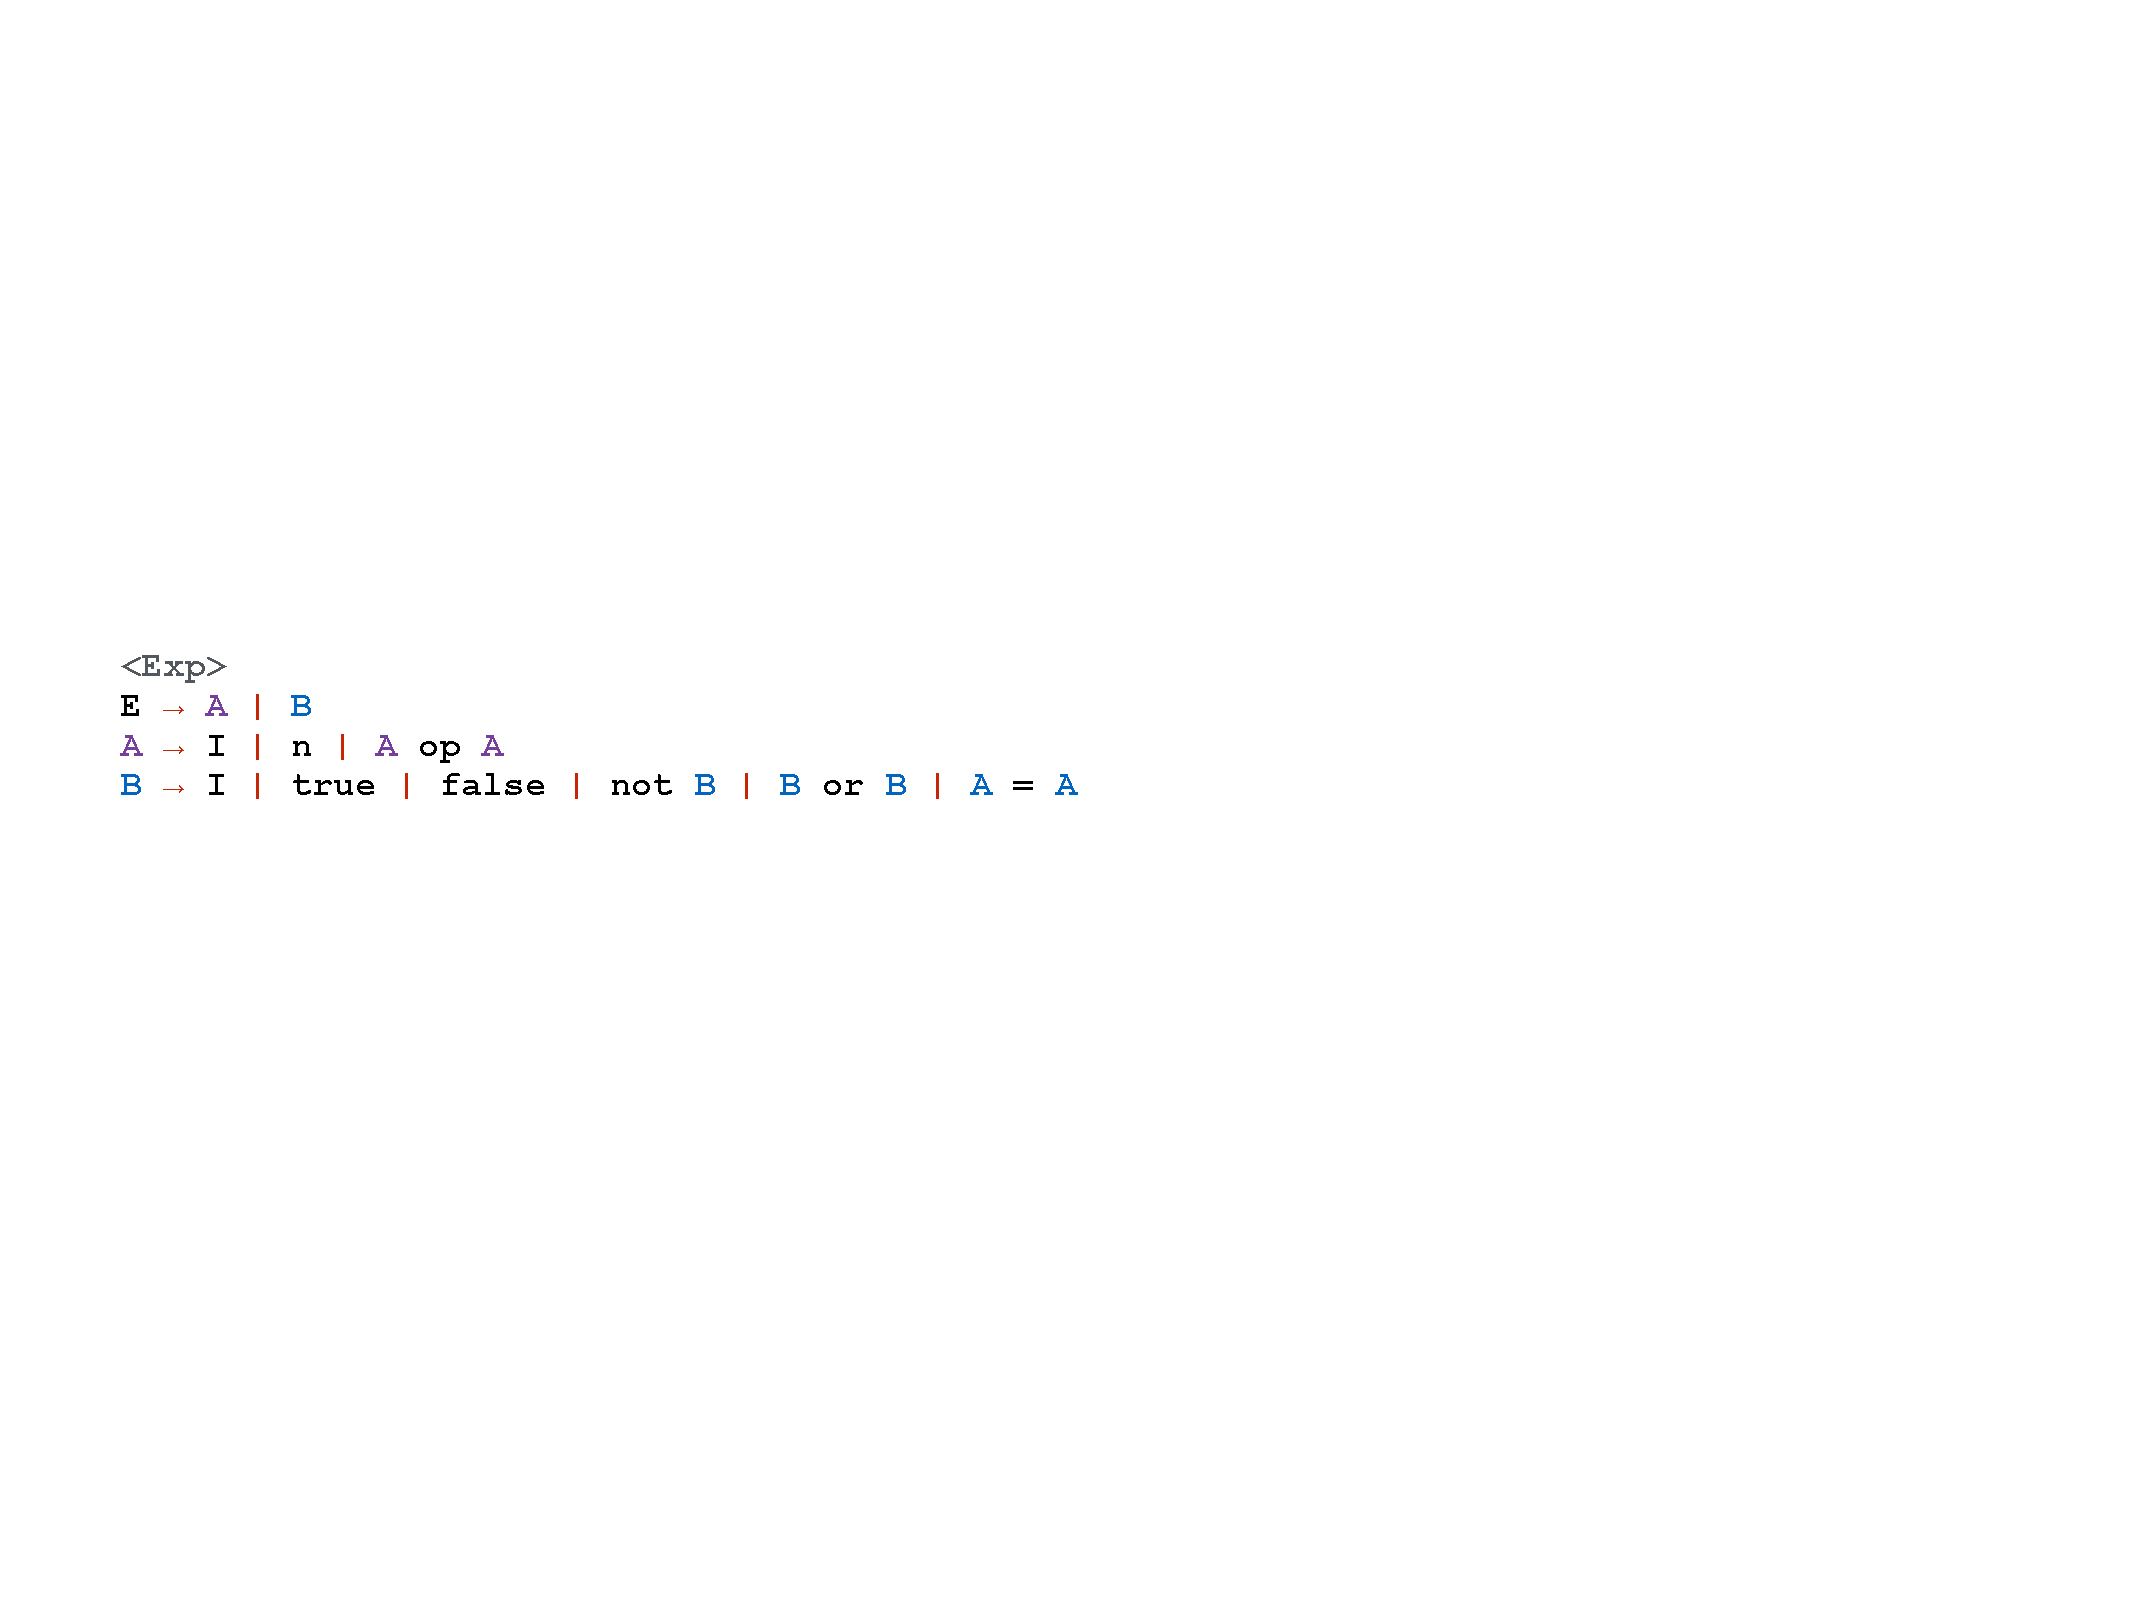
\includegraphics[width=.8\textwidth]{img/espressioni-identificatori.pdf}
	\end{figure}
	
	\noindent
	Poi si definisce l'insieme $\mathcal{E}^{V}$ delle espressioni (con identificatori) valutate ad intero o booleano. Quindi, il sistema di transizione diventa:
	\begin{equation*}
		\Gamma = \mathcal{E}^{V}, \hspace{1em} T = \mathcal{N} \cup \mathcal{B}, \hspace{1em} \mathrm{op} \in \left\{+,-,*,=\right\}, \hspace{1em} \mathrm{bop} \in \left\{=, or\right\}
	\end{equation*}
	Inoltre, le regole definite nel paragrafo \ref{regole di transizione} devono essere riscritte integrando l'ambiente. Tutte le regole $\mathcal{E}_{i}$ diventano:
	\begin{figure}[!htp]
		\centering
		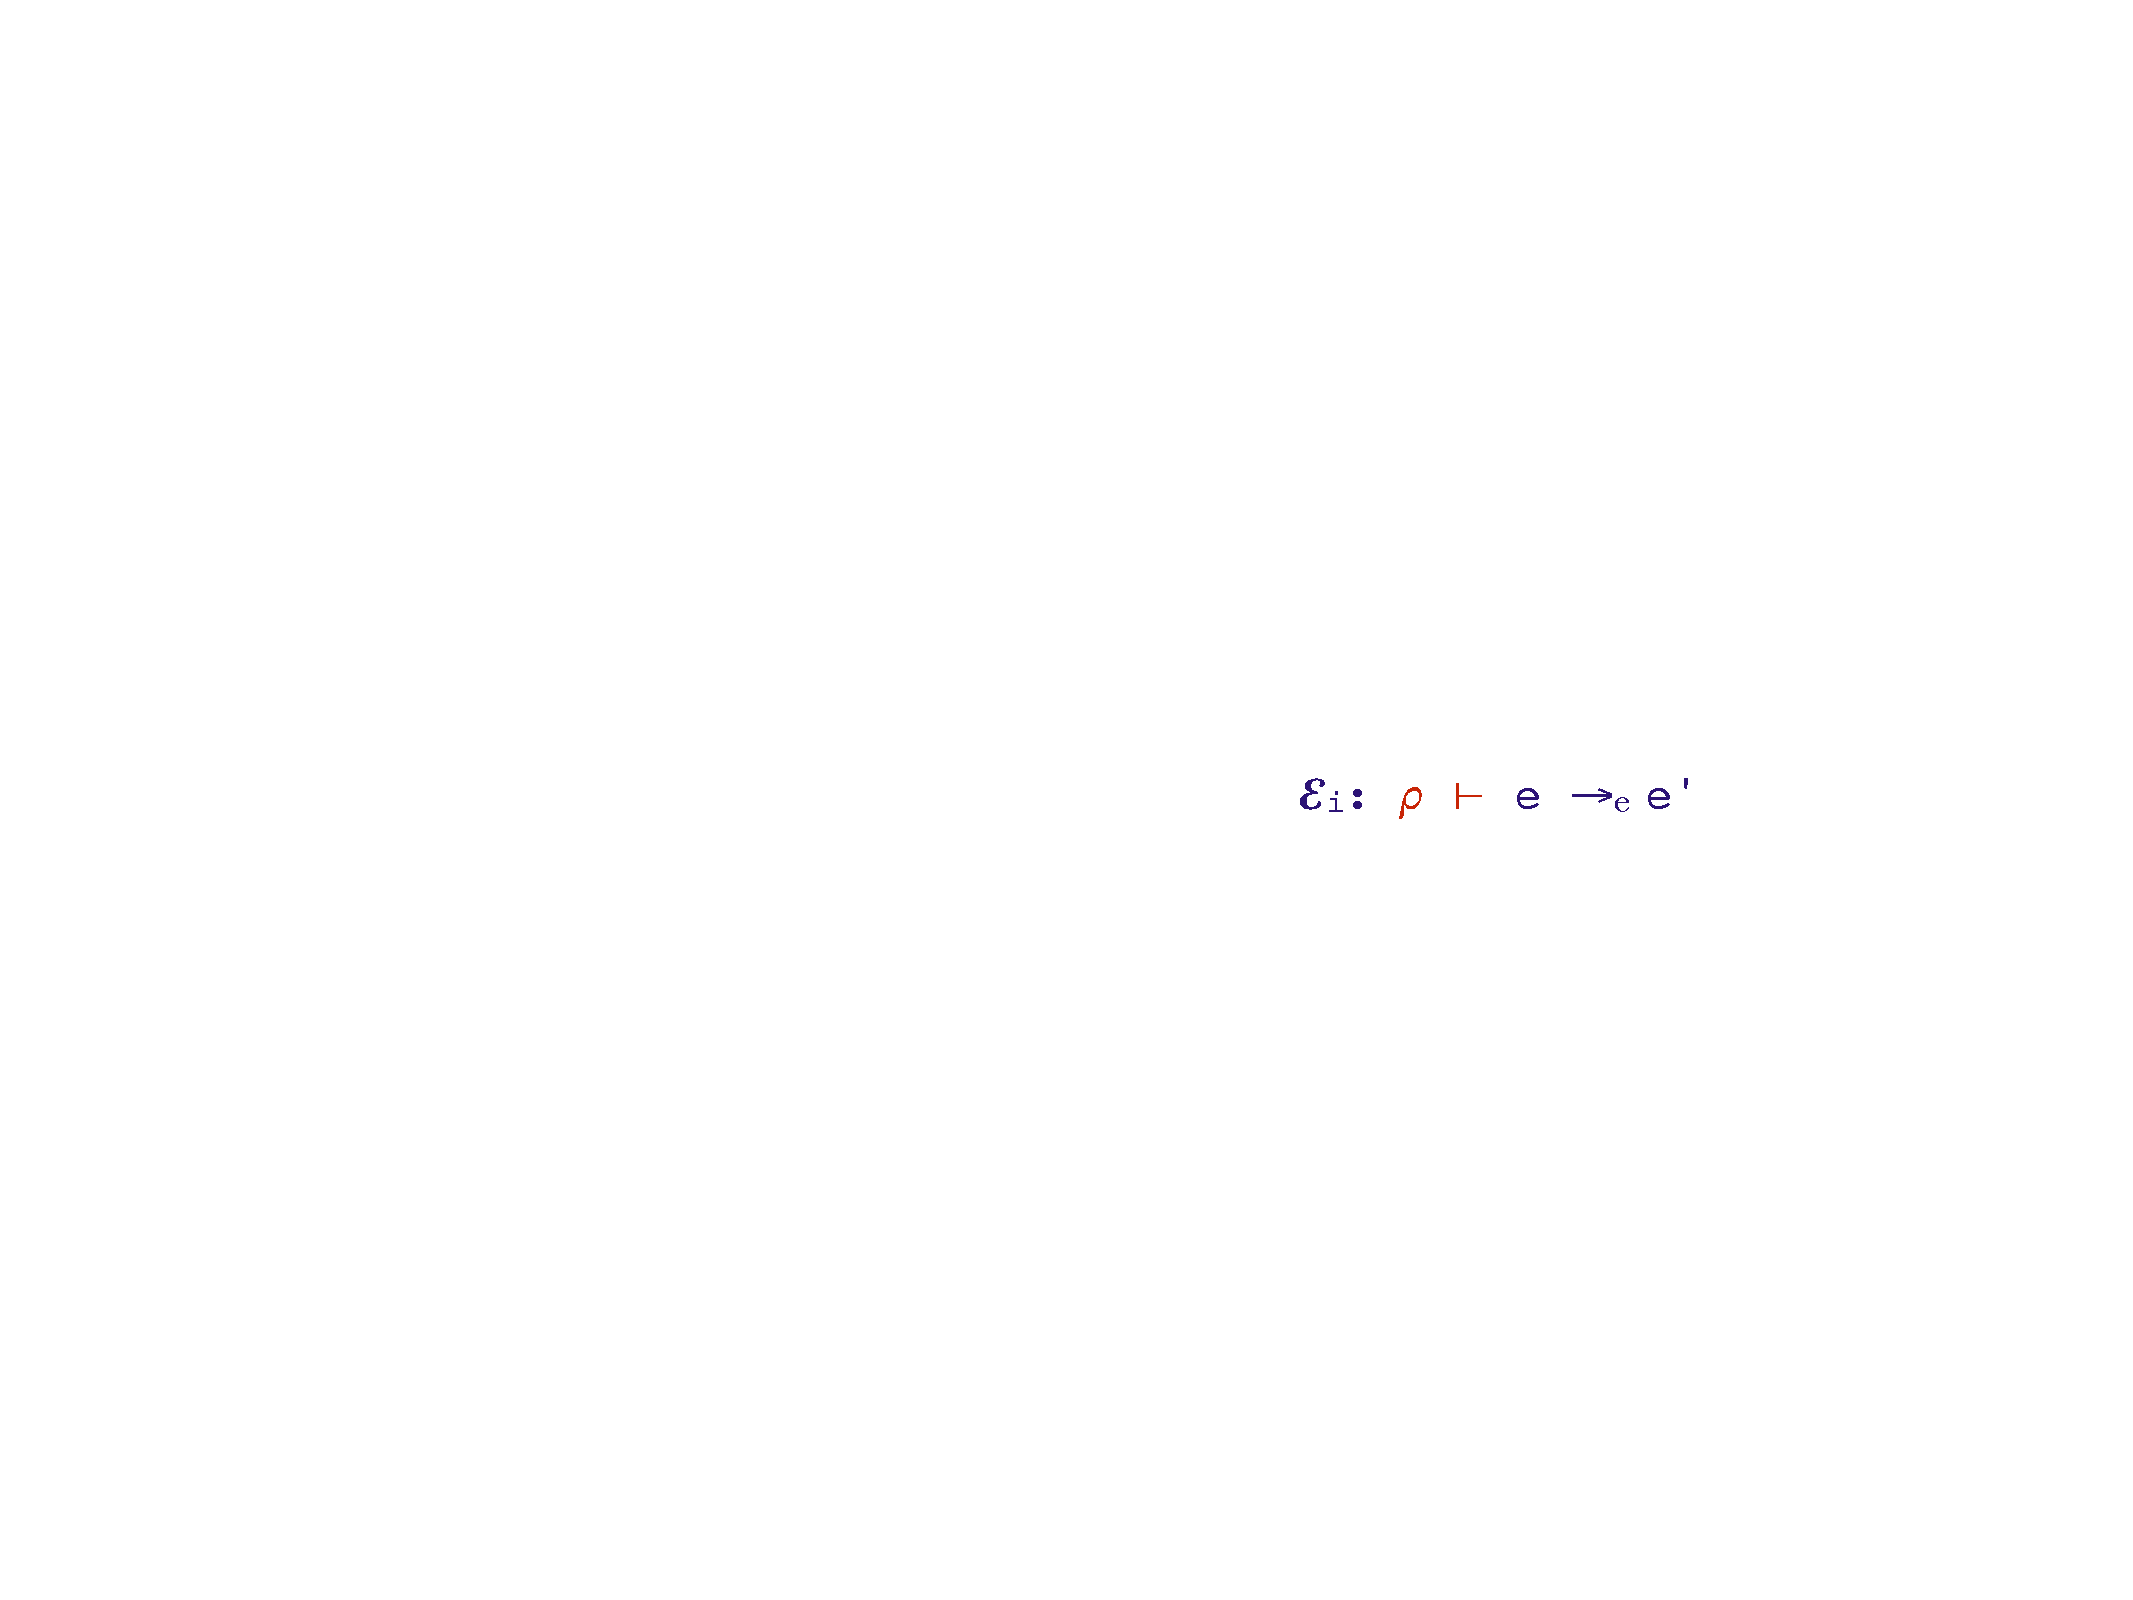
\includegraphics[width=.4\textwidth]{img/regole_arricchite.pdf}
	\end{figure}

	\noindent
	In cui $\rho$ è l'ambiente di valutazione delle espressioni, ovvero la specifica dell'associazione tra identificatori e oggetti denotati, e il pedice della freccia ($\rightarrow_{e}$) denota quale sistema di transizione si sta utilizzando.\newpage
	
	
	\subsubsection{Identificatori liberi}
	
	\begin{boxdef}
		Un identificatore è in posizione libera (\textcolor{Red3}{\textbf{occorrenza libera}}) (\textbf{\emph{free occurrence}}) se il suo uso (\emph{applied occurrence}) non è nel \textbf{raggio di azione (scope)} di una definizione.
	\end{boxdef}\newpage
	
	
	\subsection{Nuove regole}\label{nuove regole}
	
	Per una descrizione dettagliata delle regole si rimanda al paragrafo \ref{regole di transizione}:
	\begin{itemize}
		\item La prima regola:
		\begin{figure}[!htp]
			\centering
			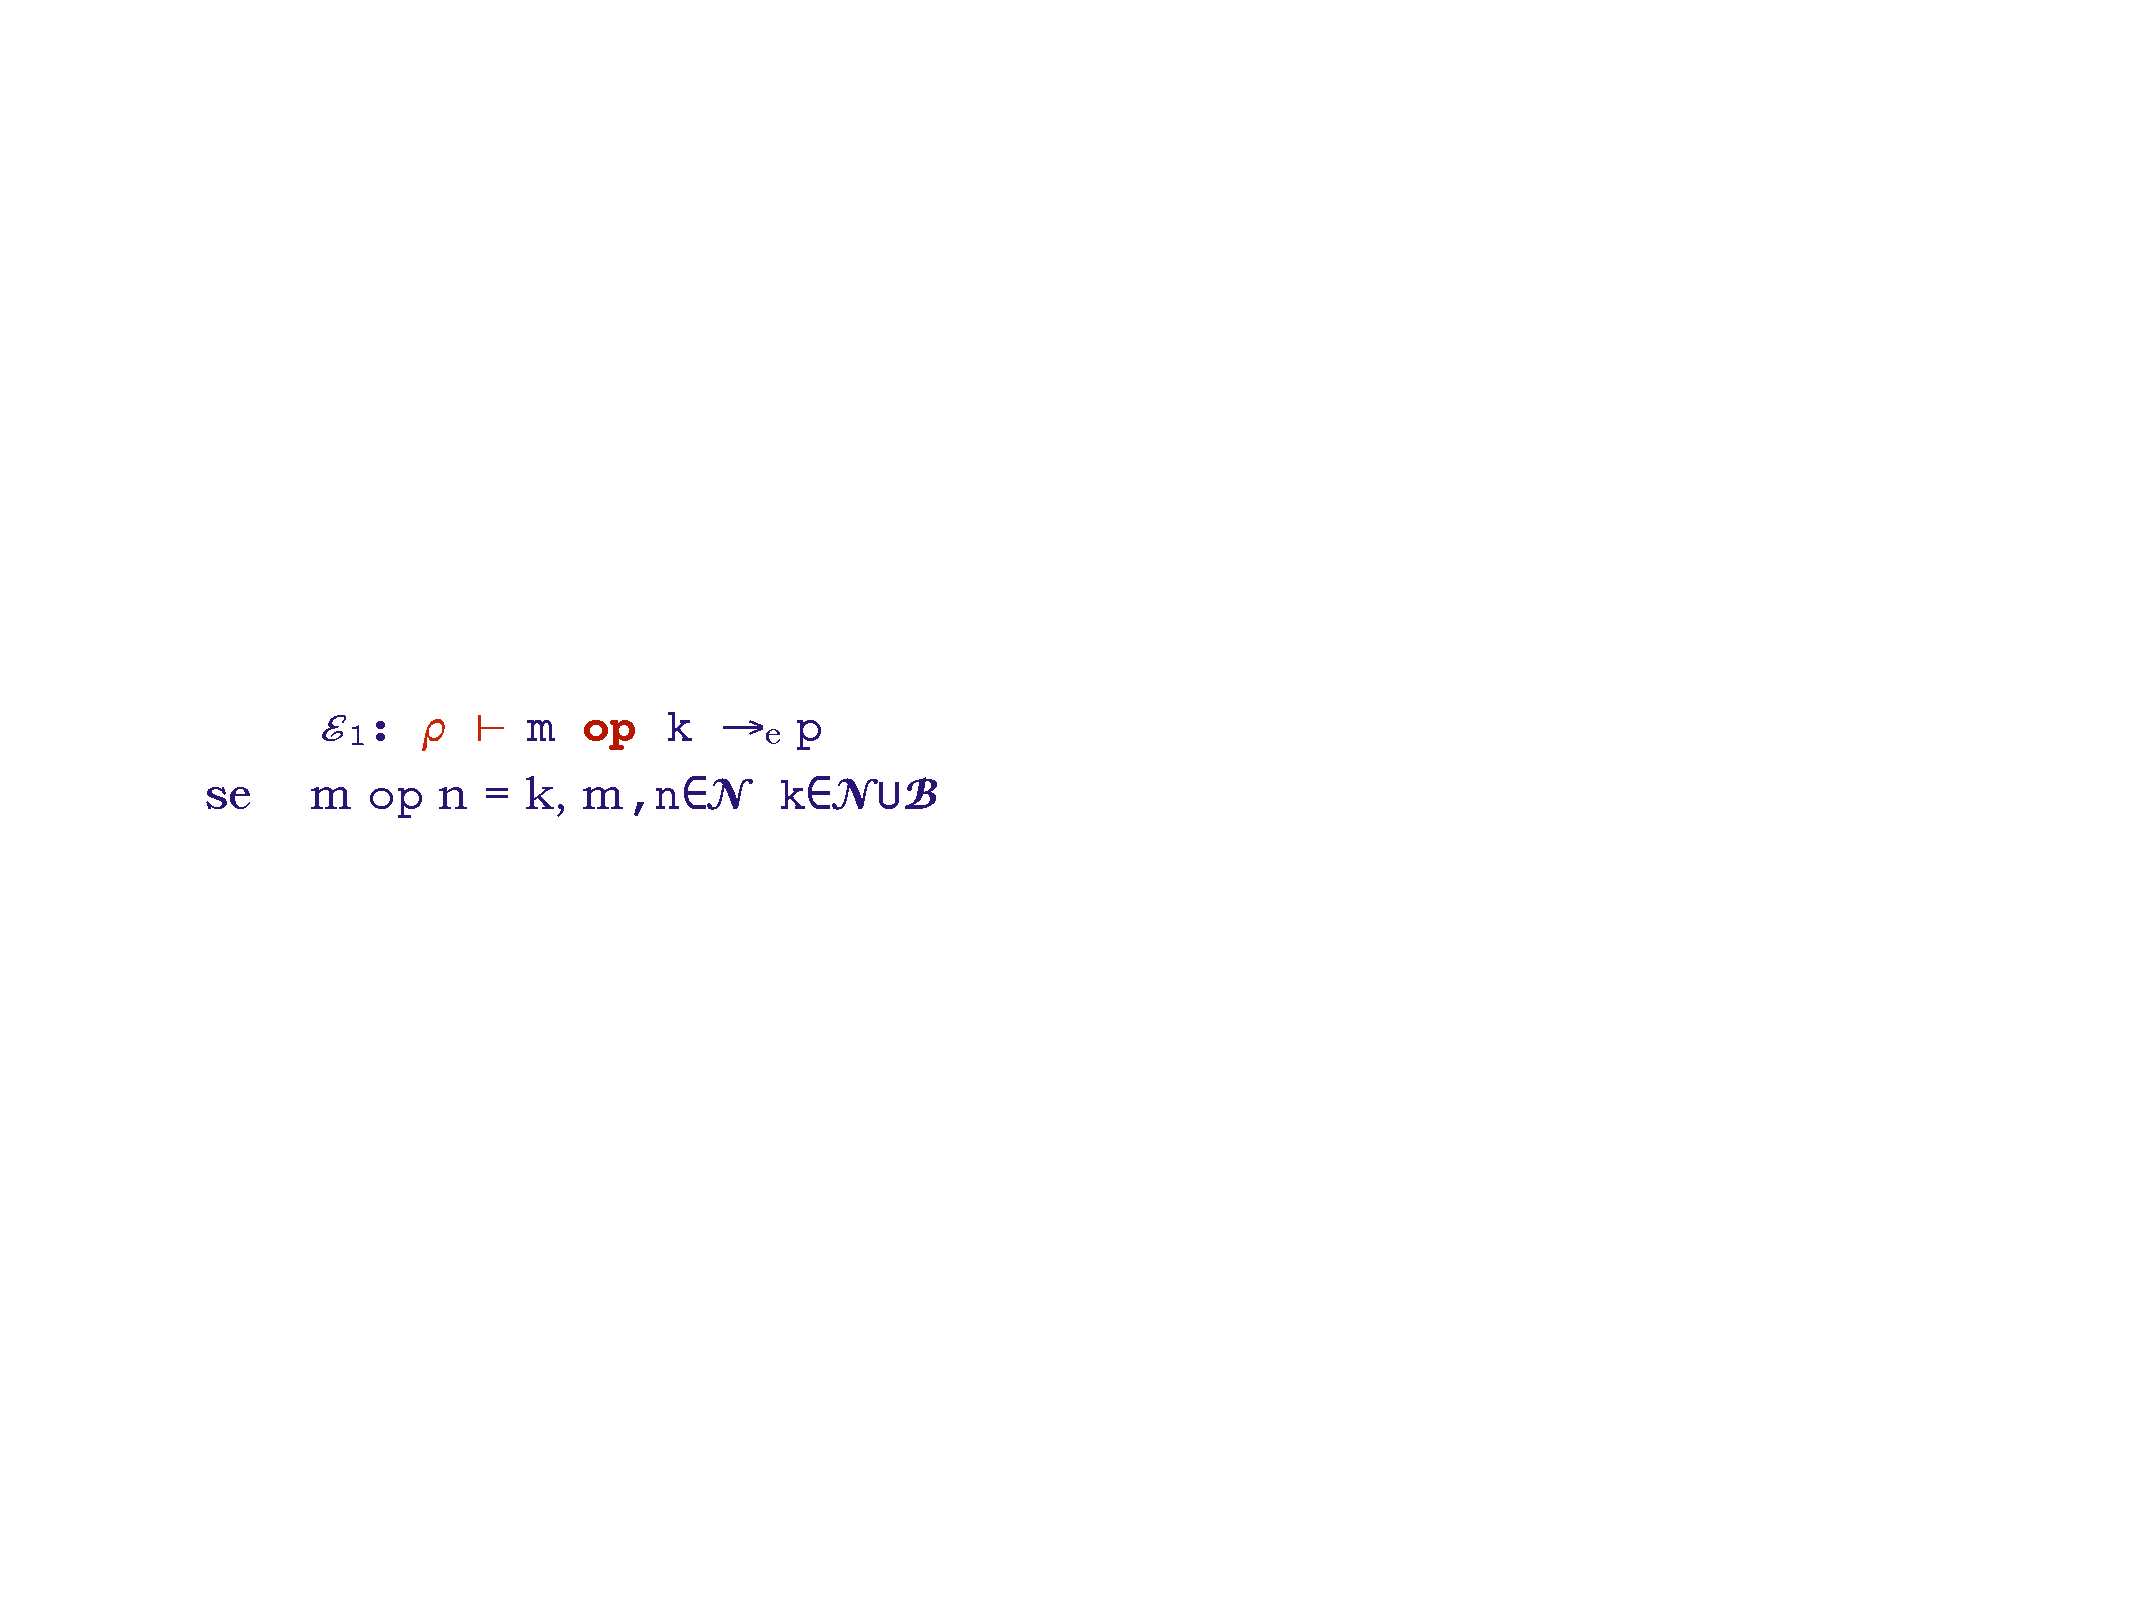
\includegraphics[width=.6\textwidth]{img/regola_espressione-1.pdf}
		\end{figure}
		
		\item La seconda regola cambia, in quanto ora è necessario l'assioma per gli identificatori. In questo \textbf{assioma}, quando si incontra un identificatore, questo viene valutato nel valore che l'ambiente associa all'identificatore. Ovviamente, questa regola è applicabile solo se $I$ è un identificatore per il quale $\rho$ esiste un'associazione.
		\begin{figure}[!htp]
			\centering
			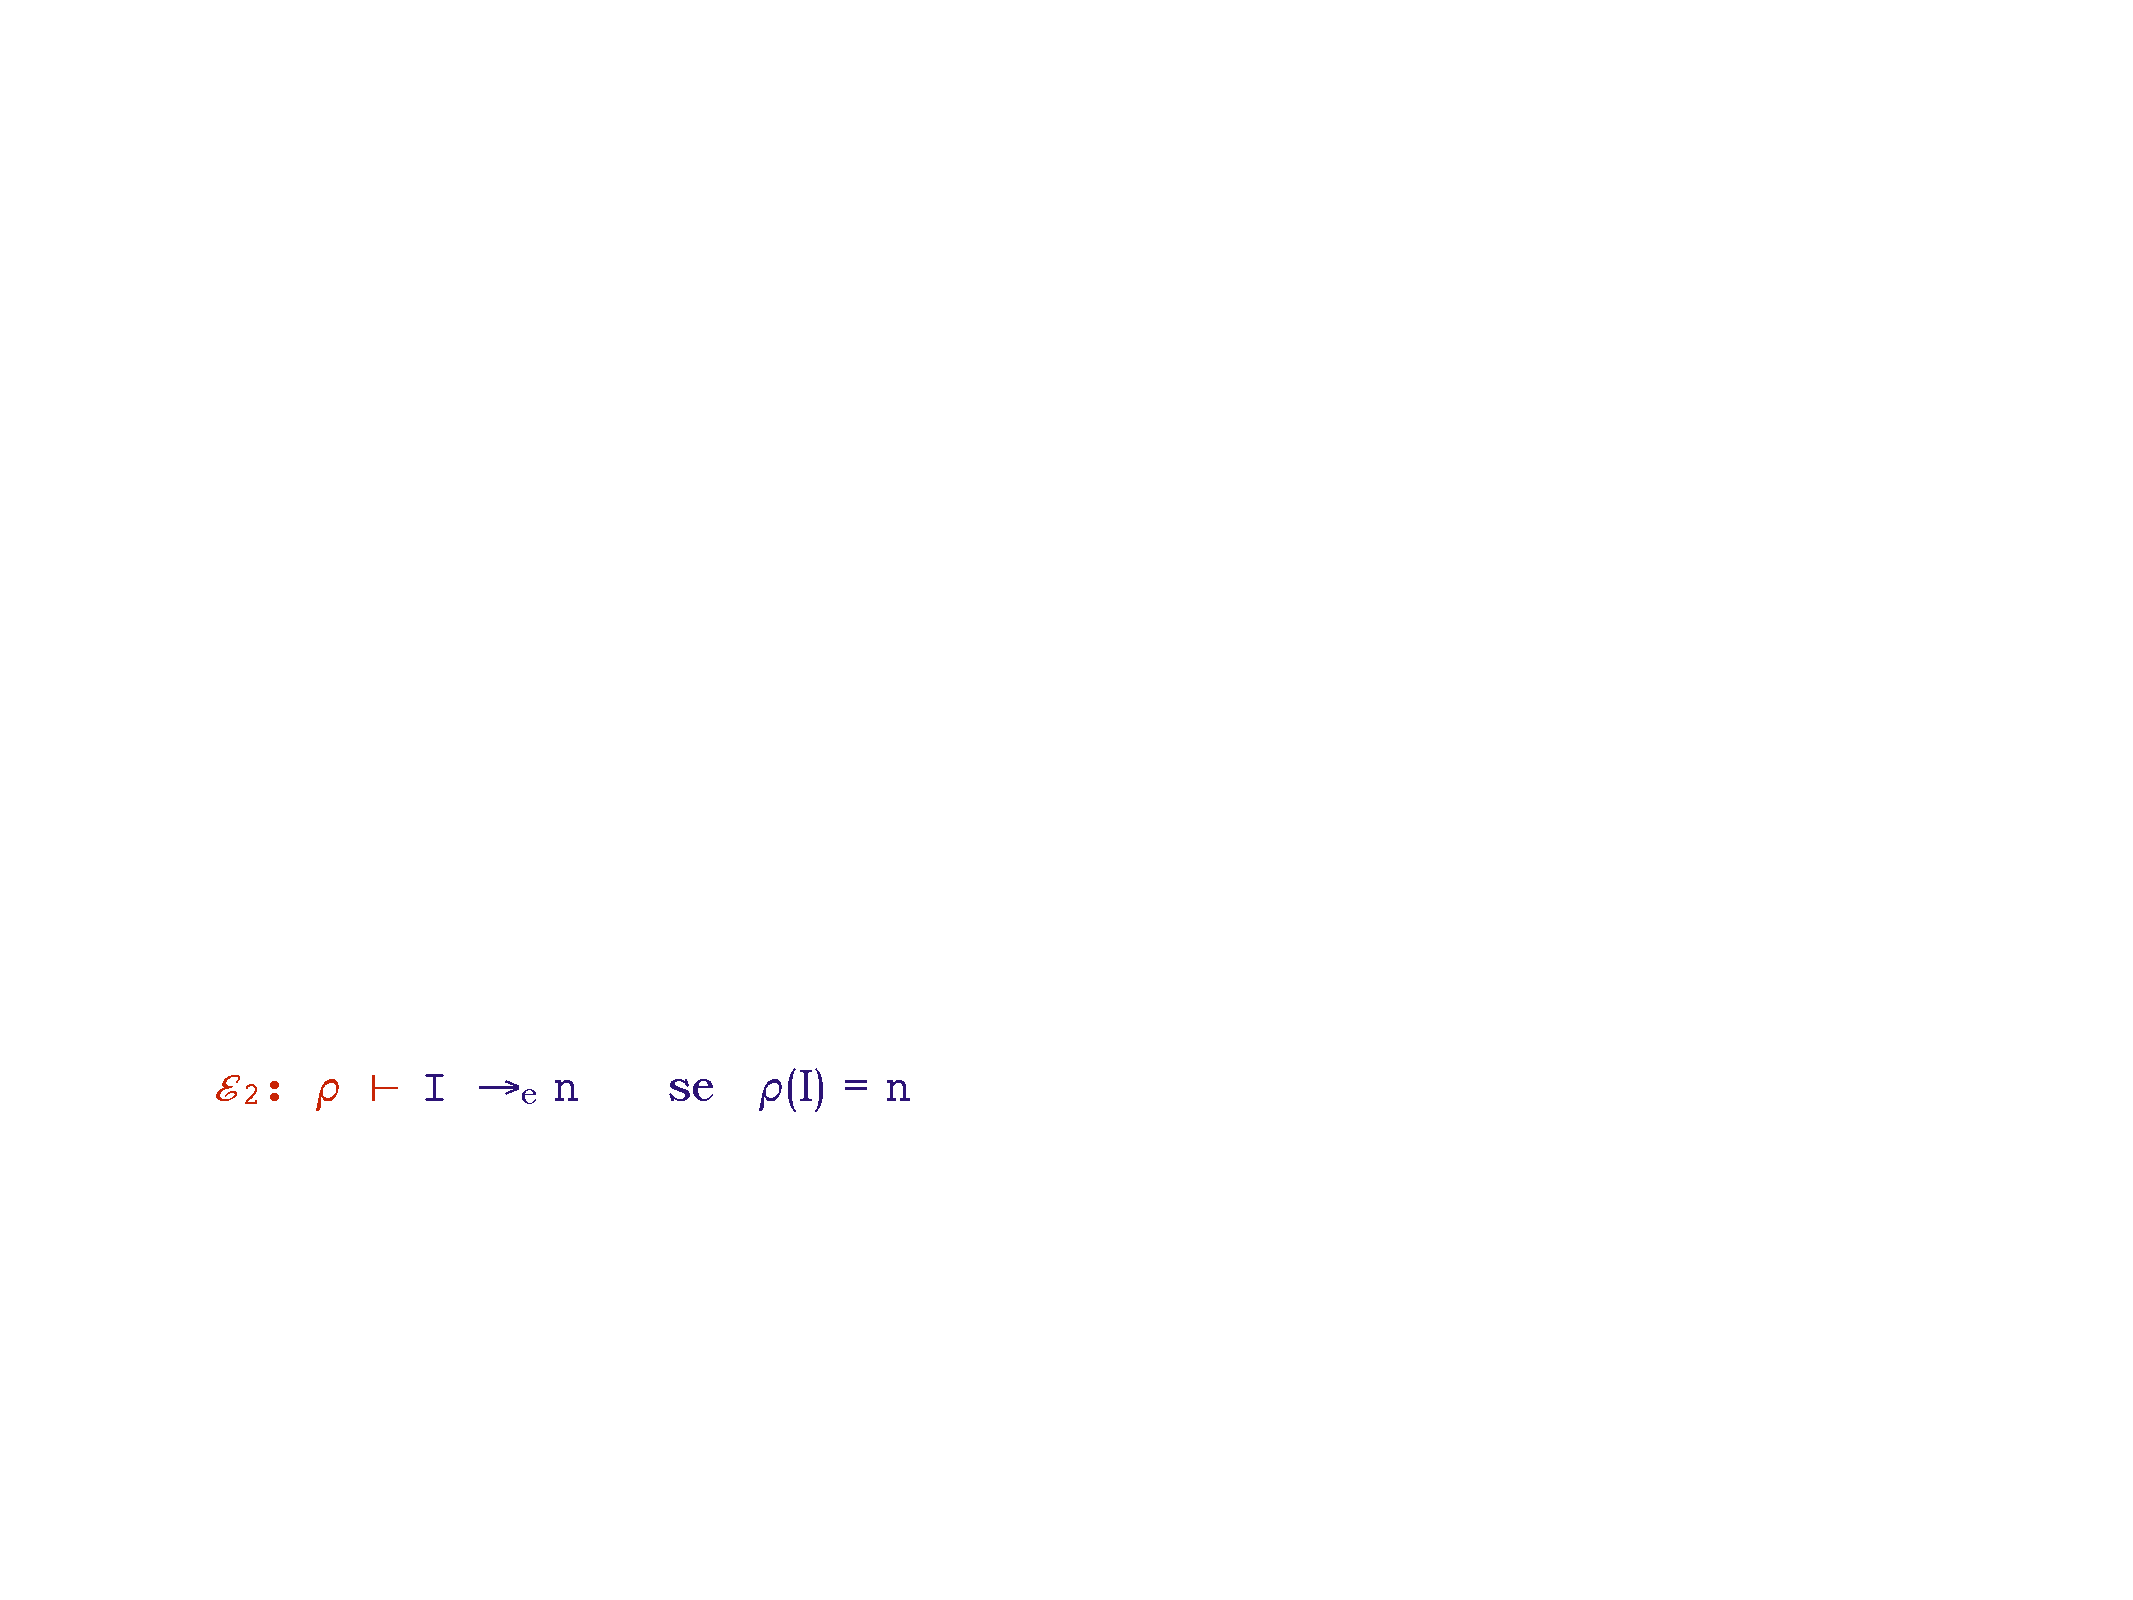
\includegraphics[width=.6\textwidth]{img/regola_espressione-2.pdf}
		\end{figure}
		
		\item La terza regola:
		\begin{figure}[!htp]
			\centering
			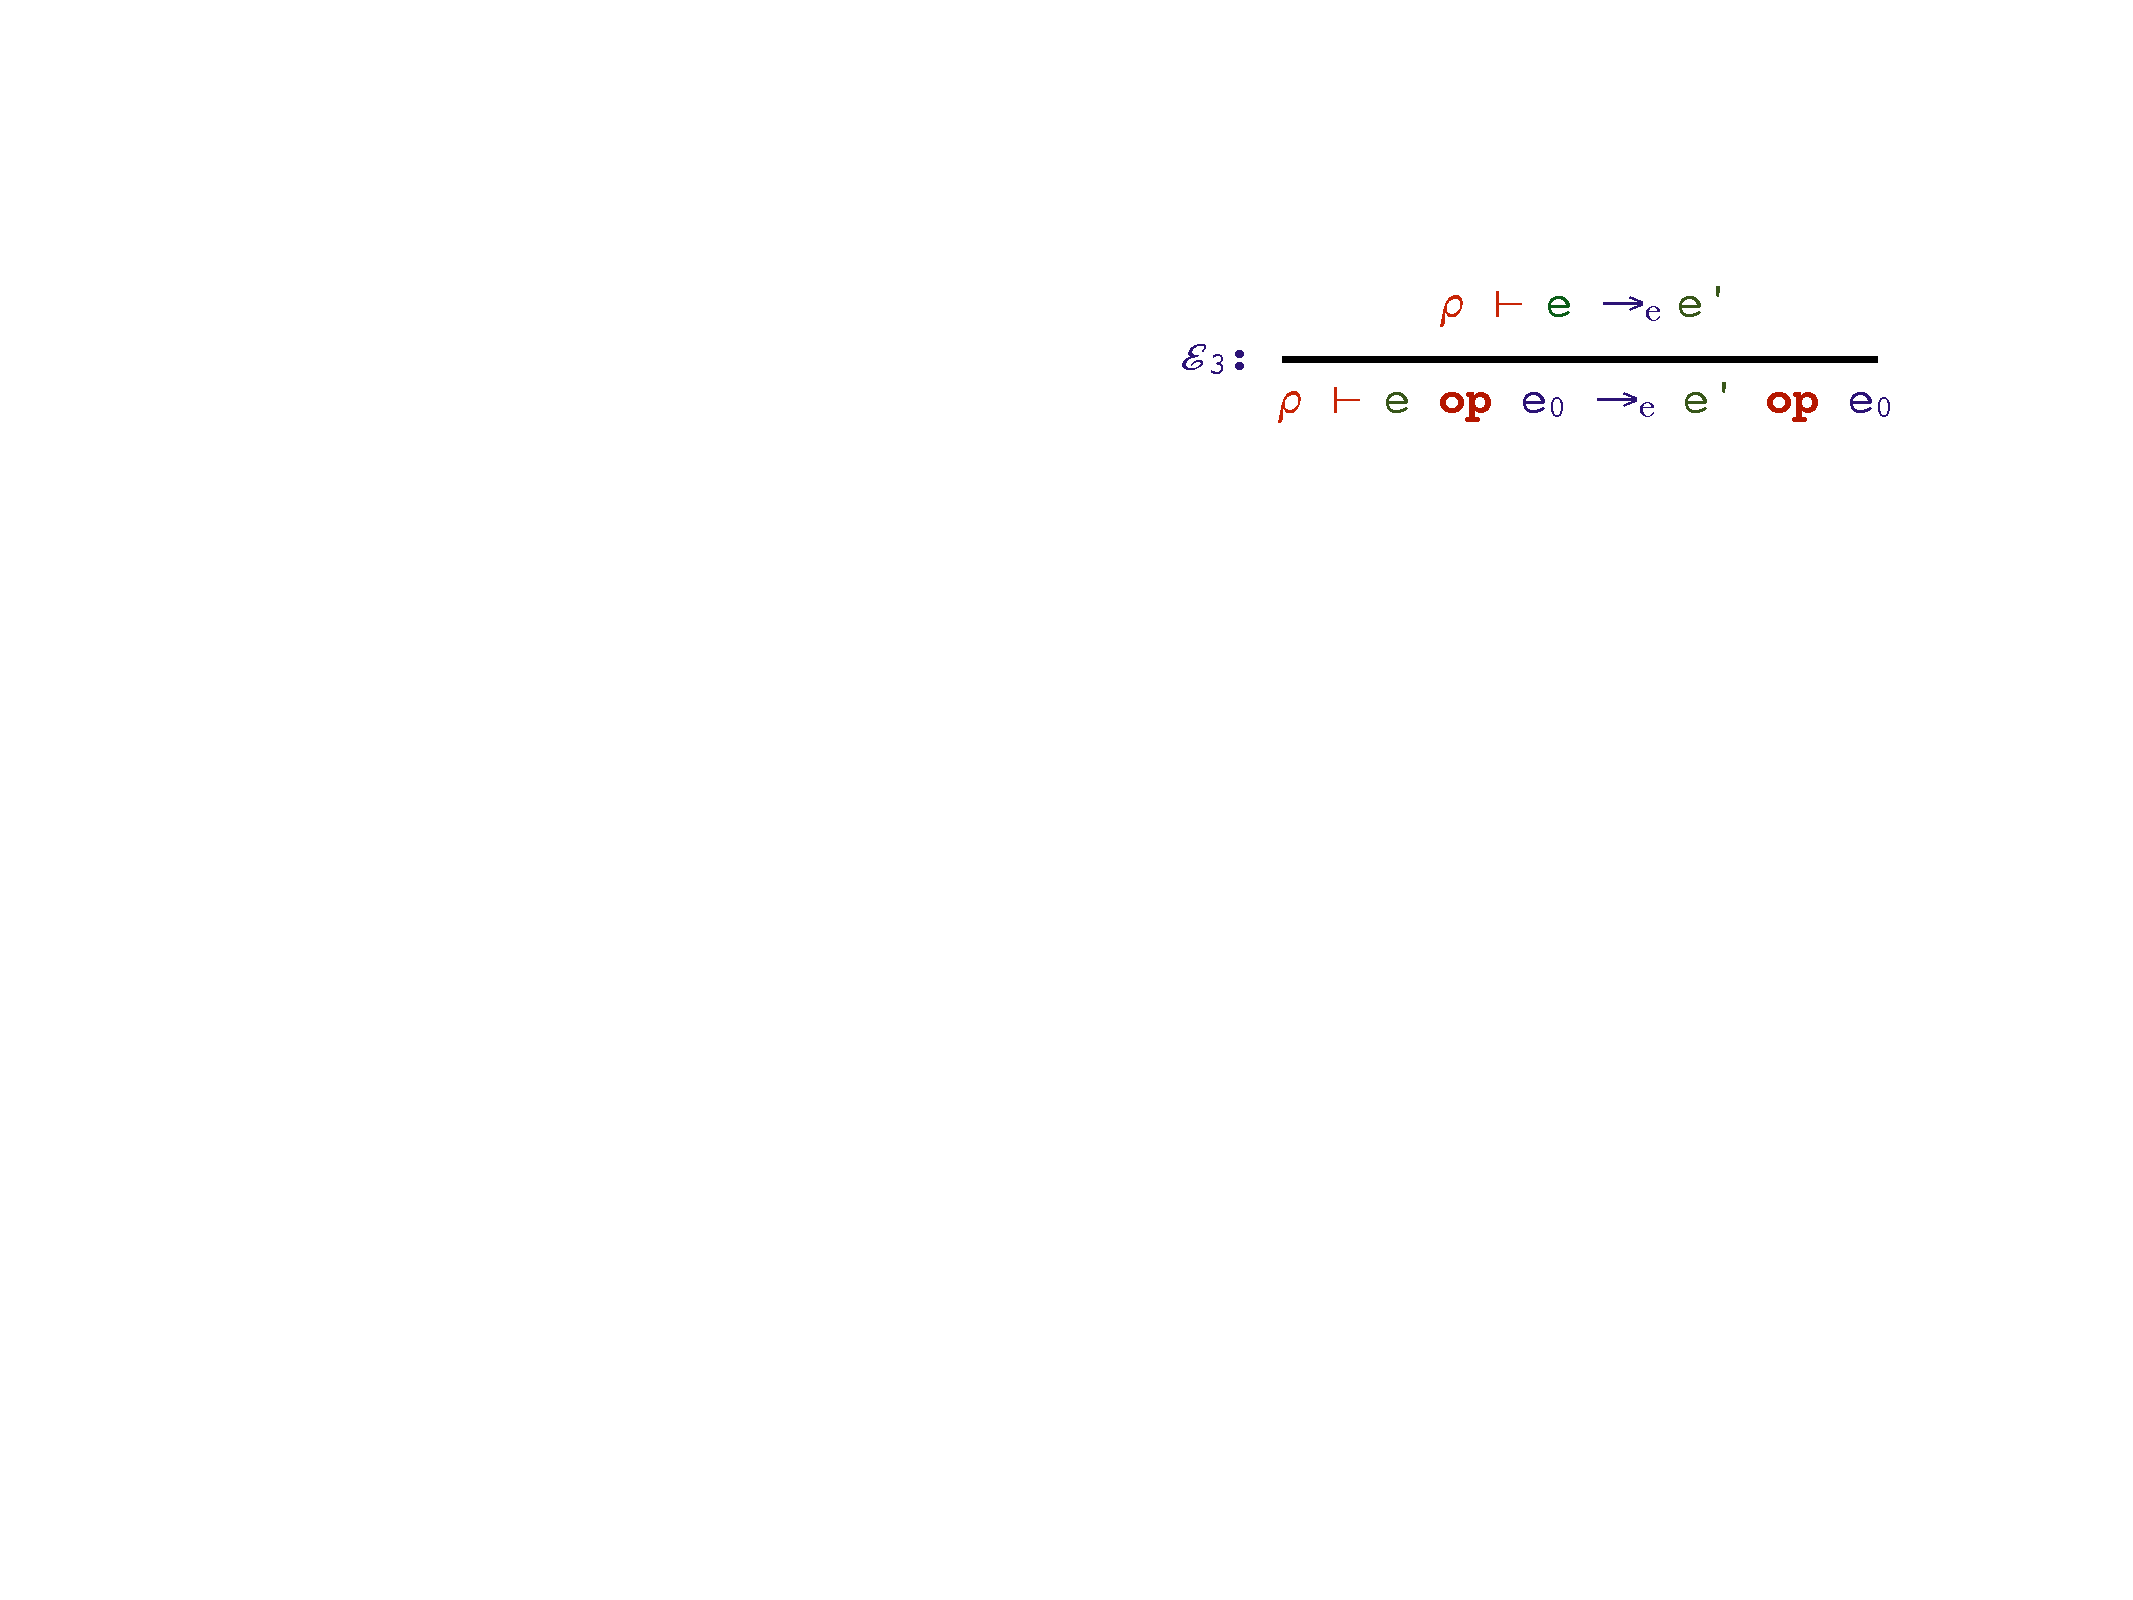
\includegraphics[width=.6\textwidth]{img/regola_espressione-3.pdf}
		\end{figure}
		
		\item La quarta regola:
		\begin{figure}[!htp]
			\centering
			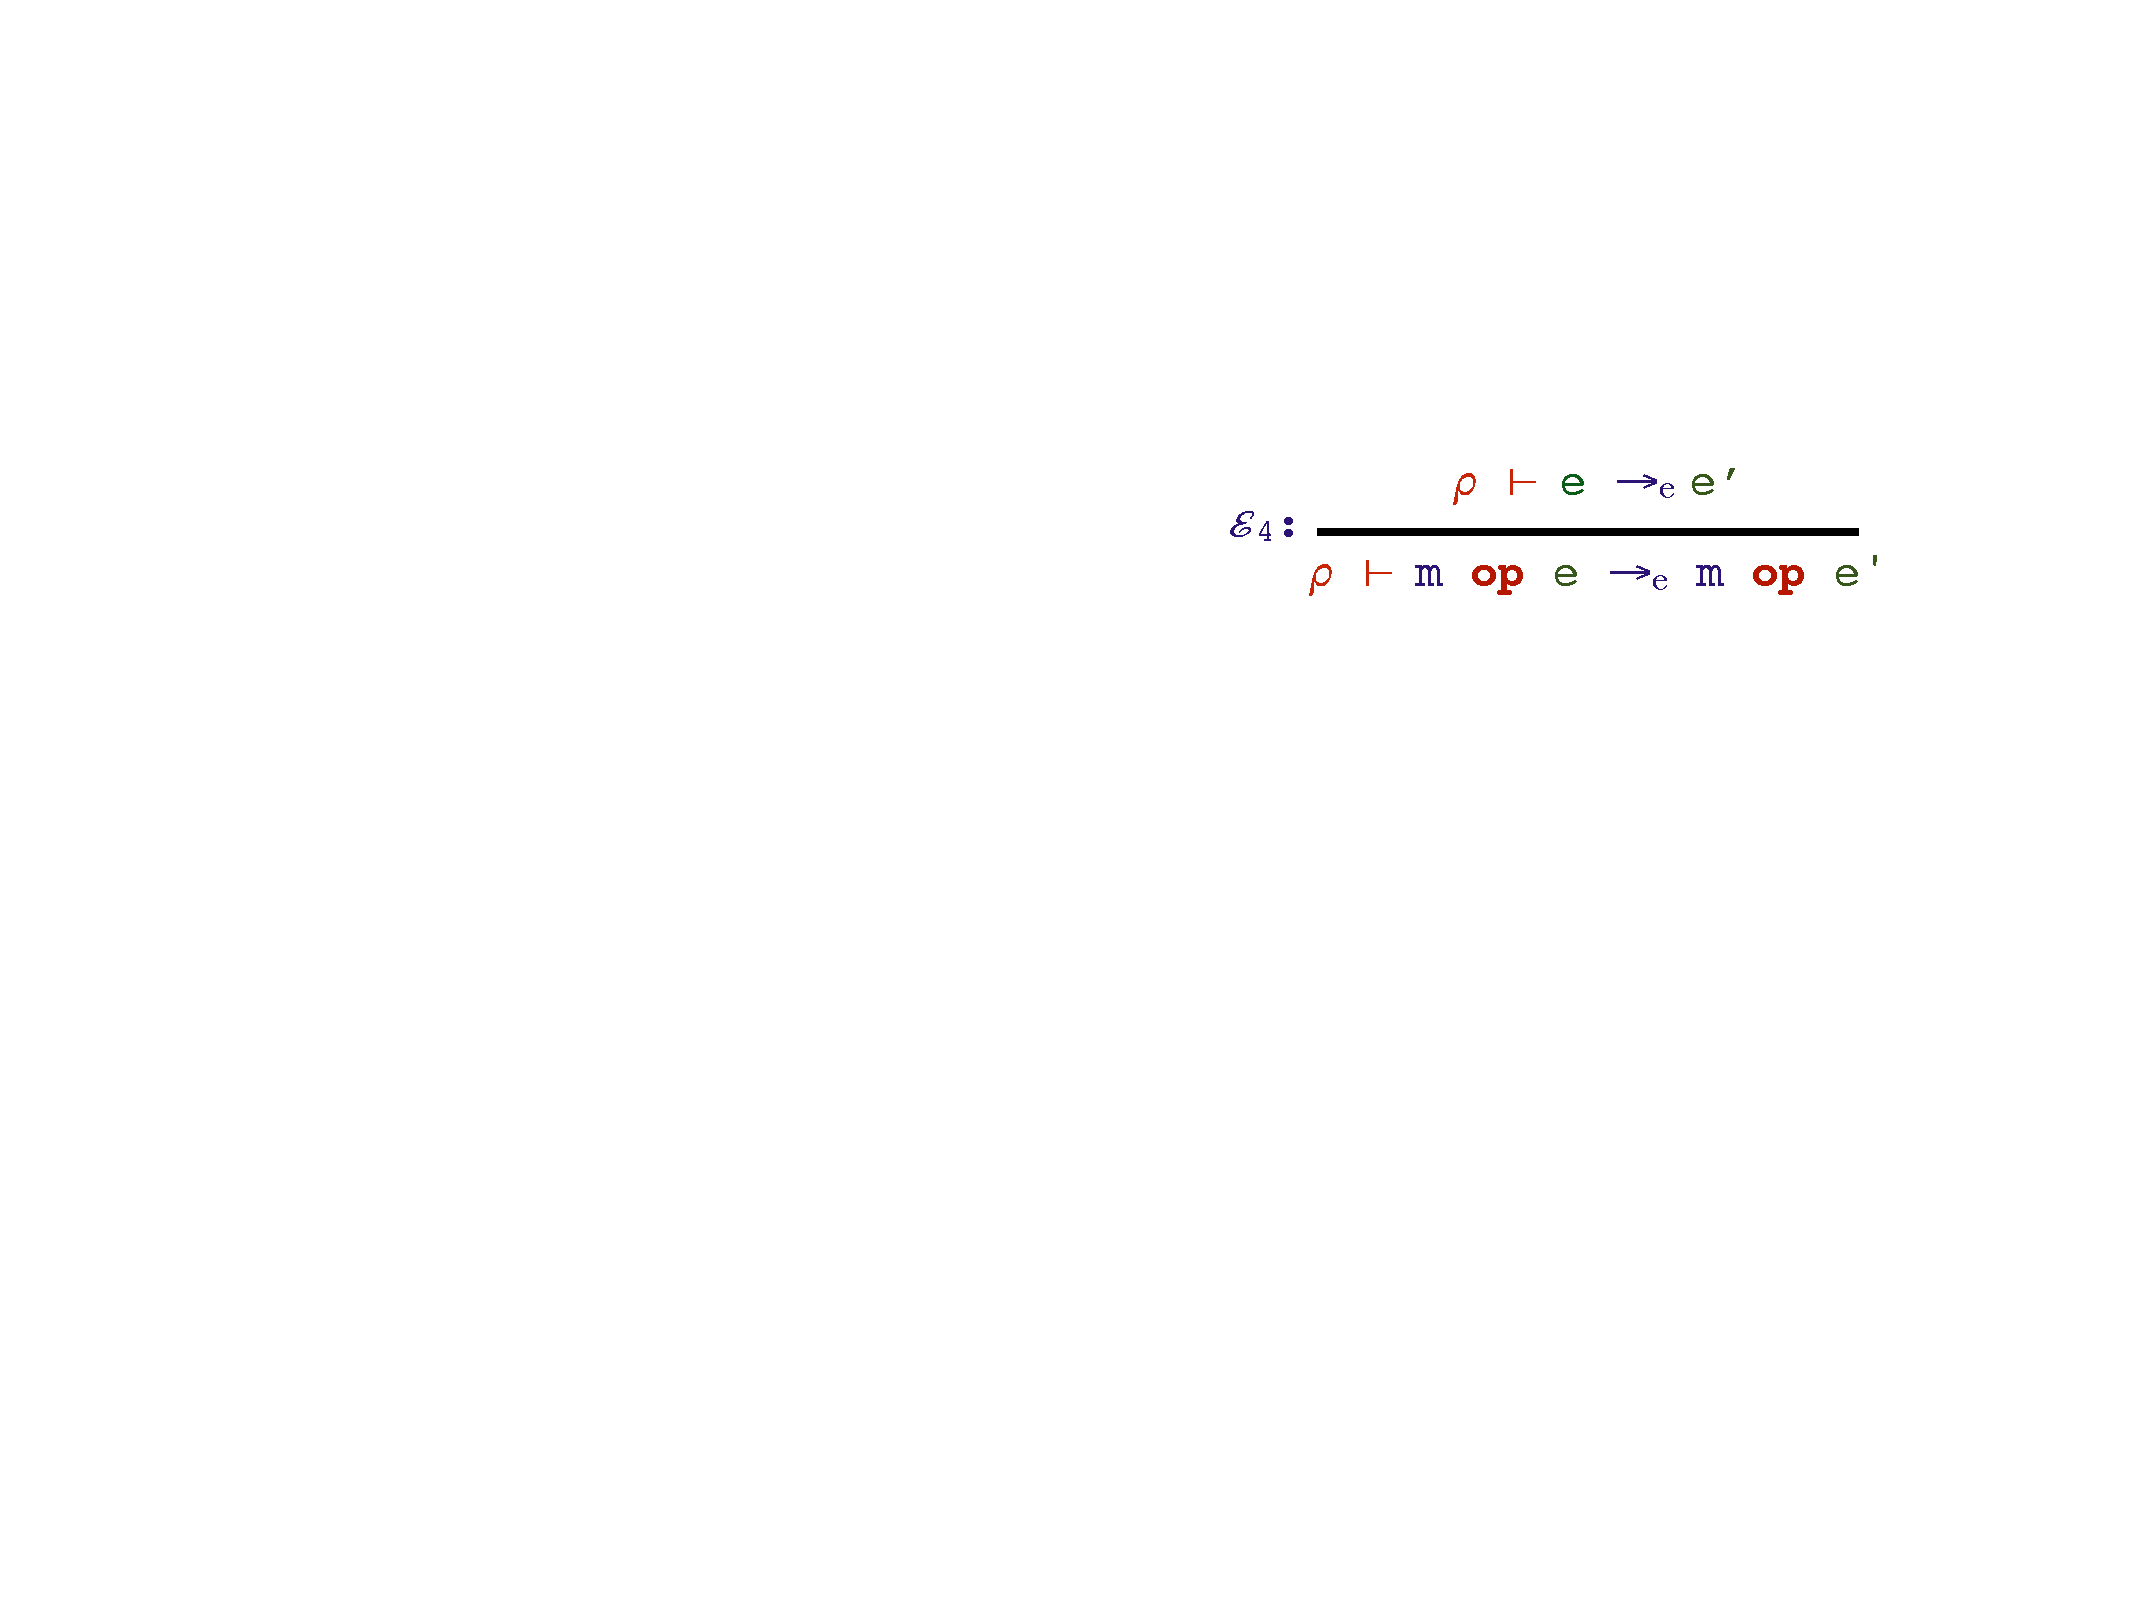
\includegraphics[width=.6\textwidth]{img/regola_espressione-4.pdf}
		\end{figure}
		
		\item La quinta regola:
		\begin{figure}[!htp]
			\centering
			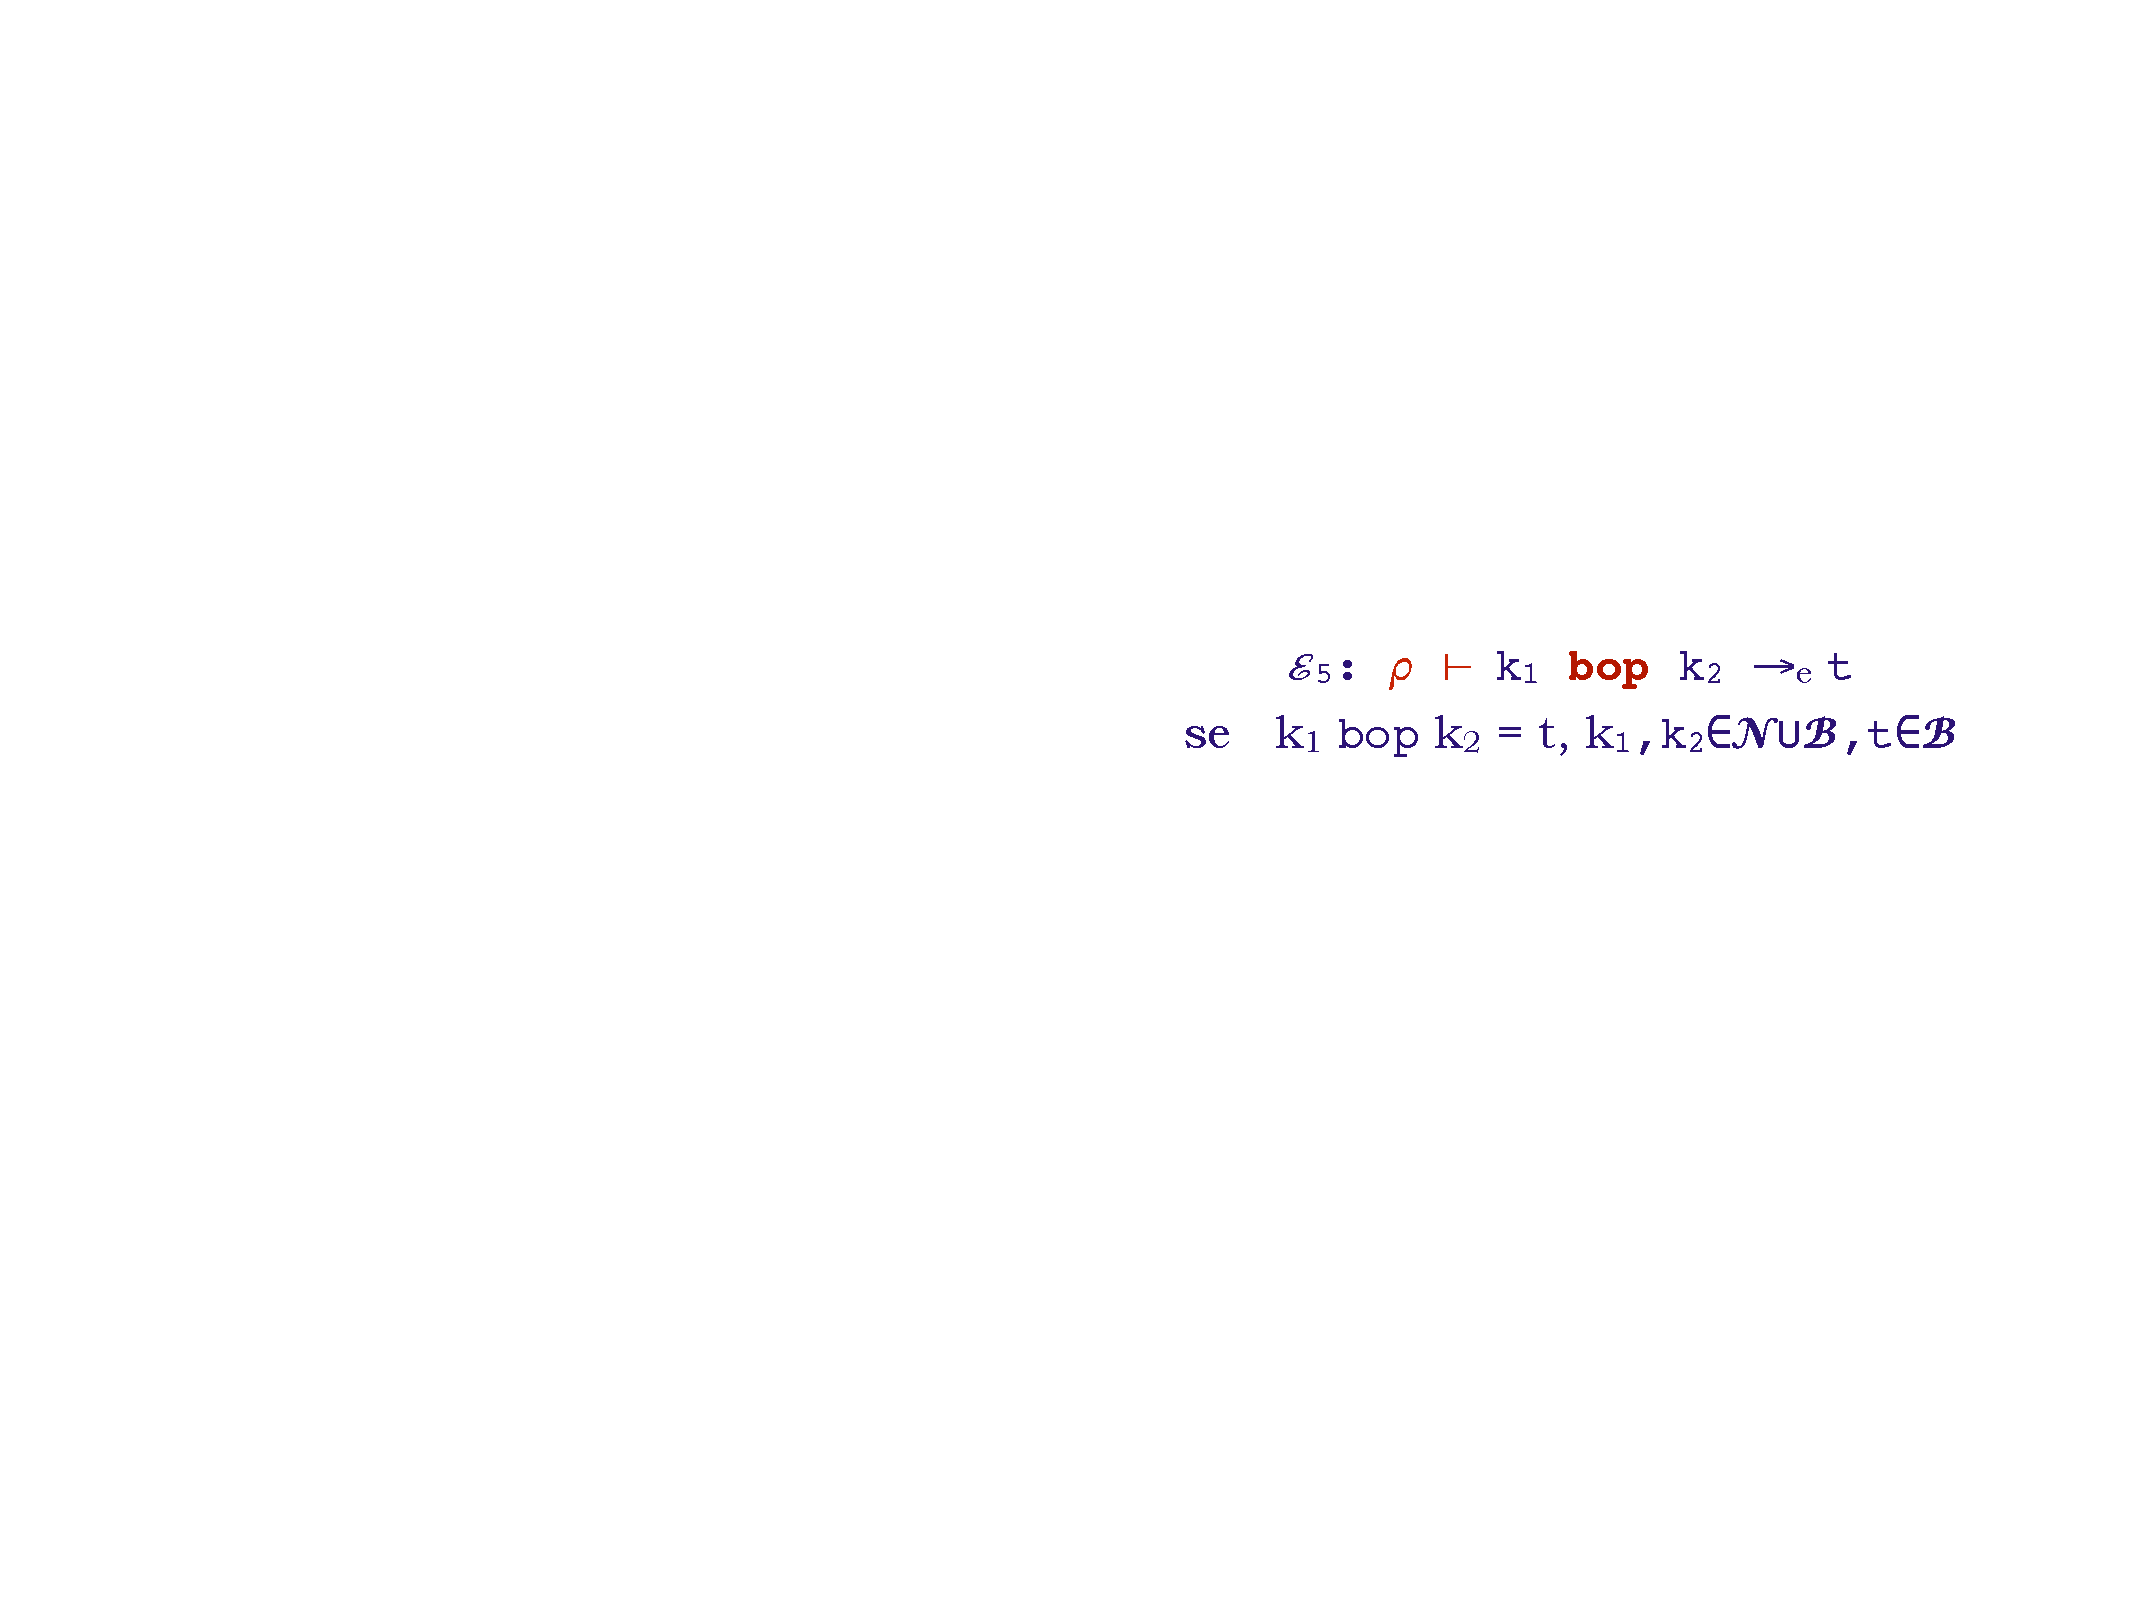
\includegraphics[width=.6\textwidth]{img/regola_espressione-5.pdf}
		\end{figure}
		
		\item La terza regola aggiornata:
		\begin{figure}[!htp]
			\centering
			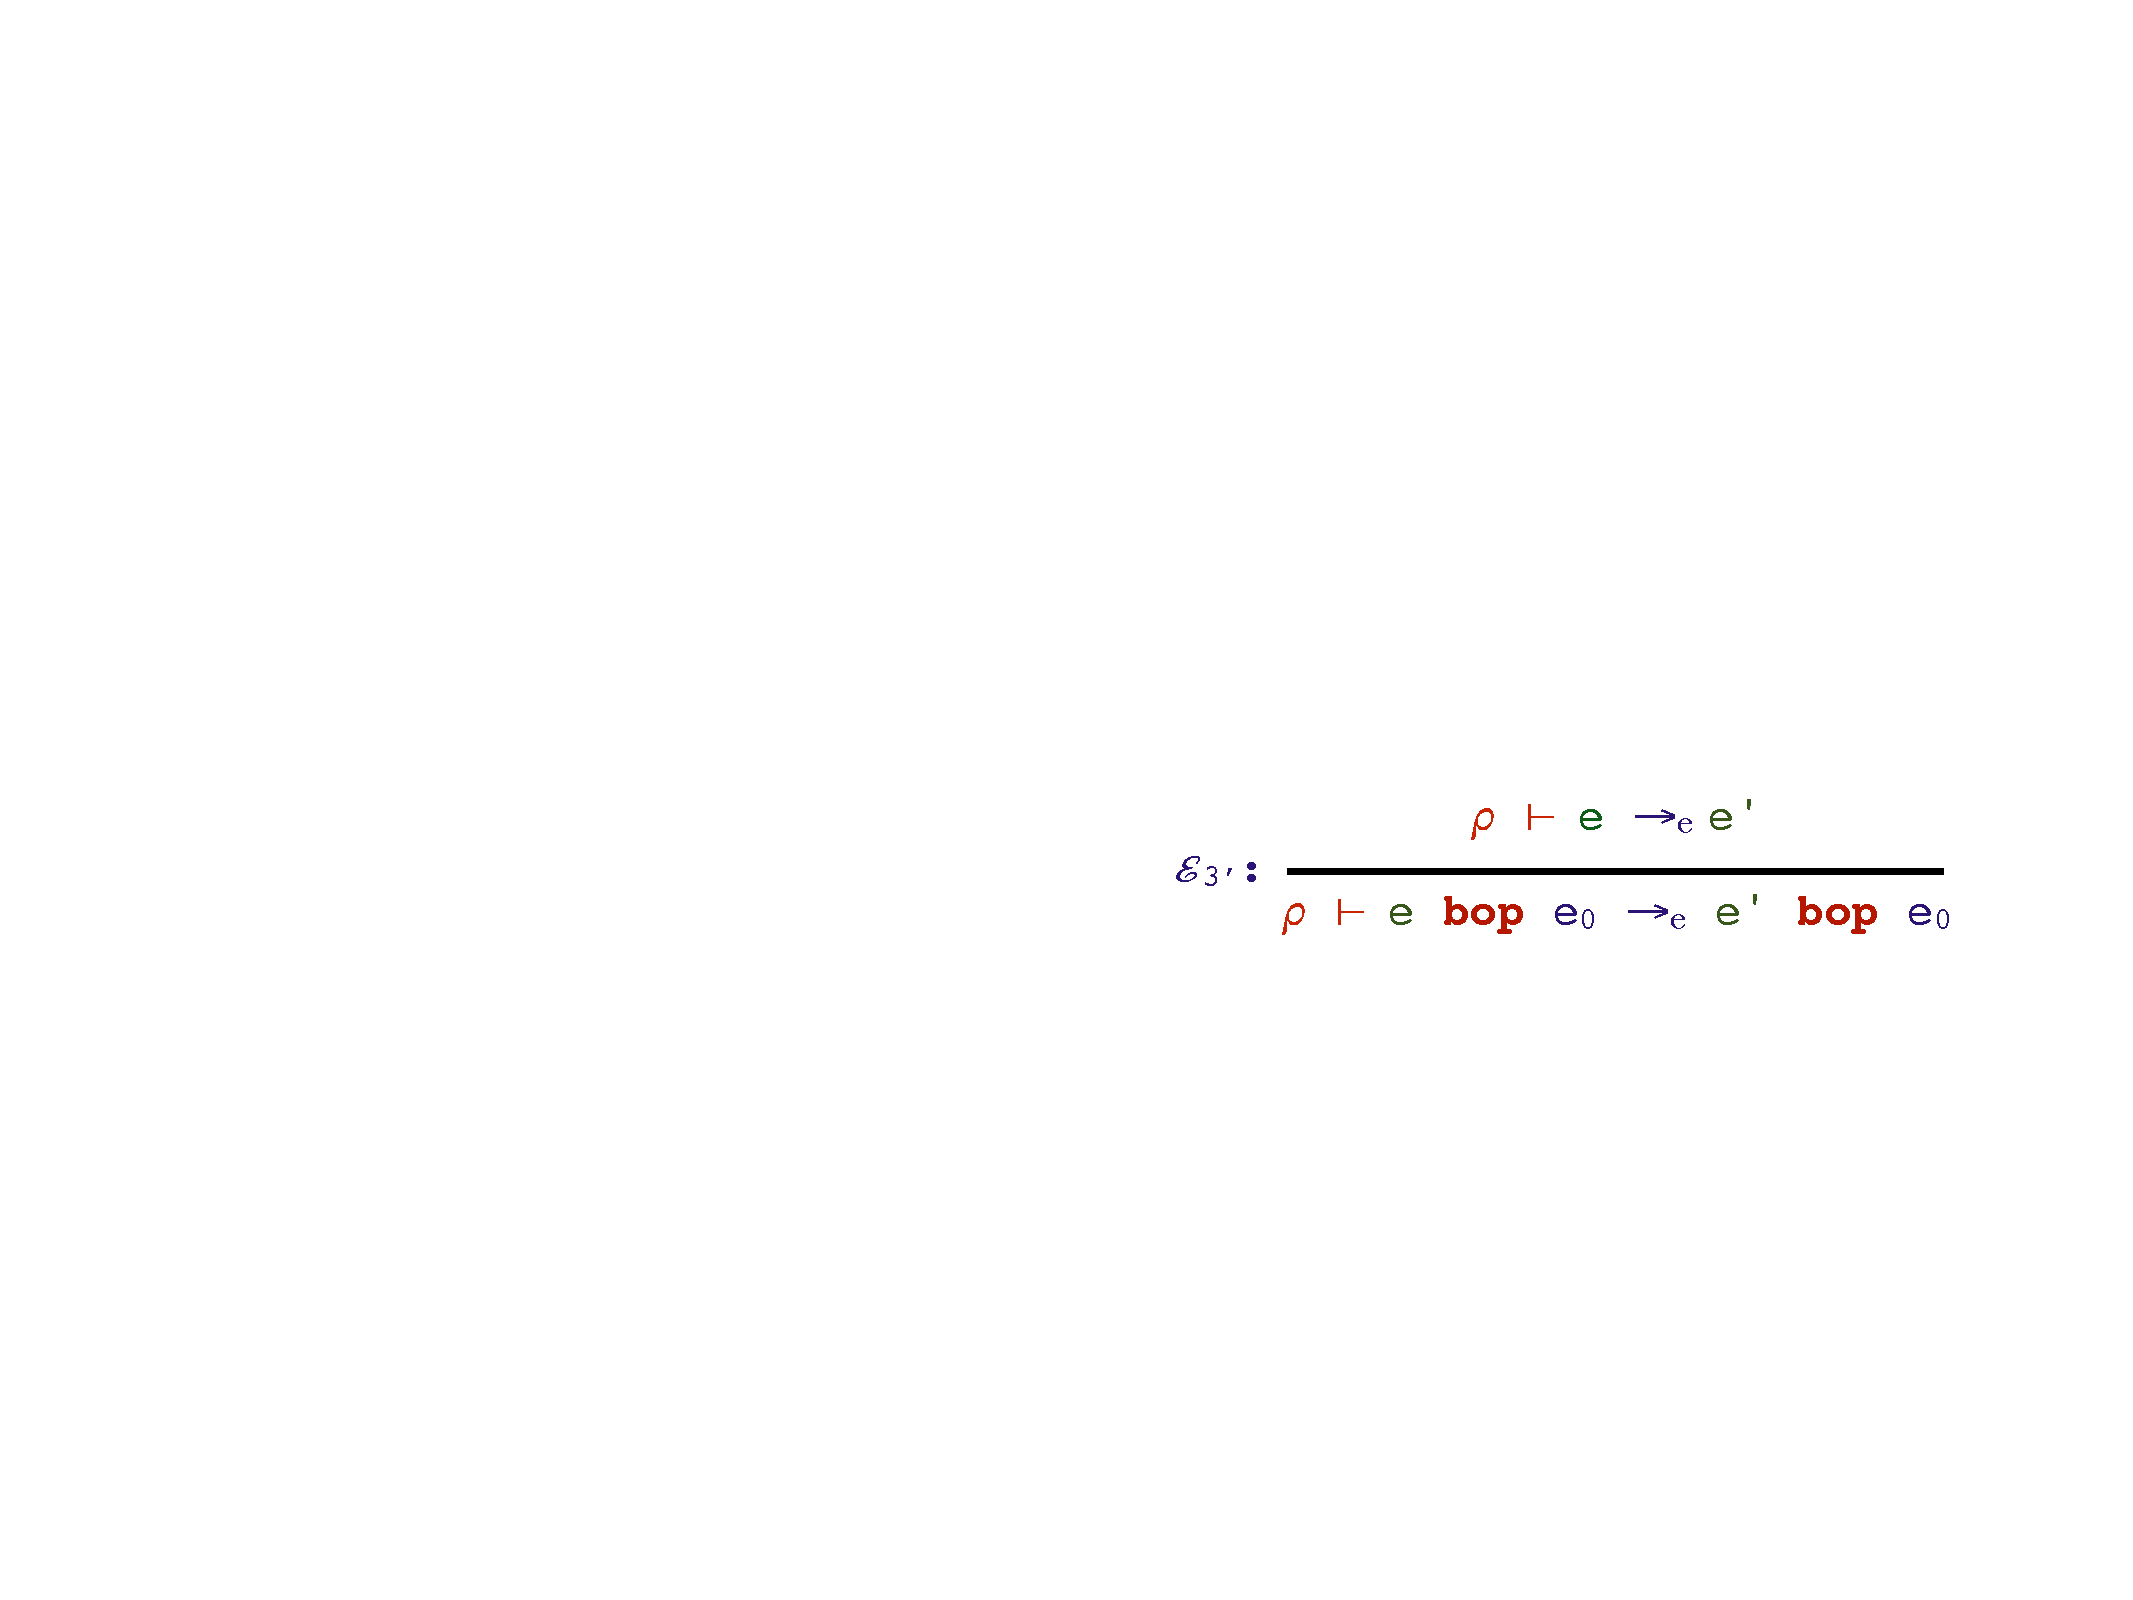
\includegraphics[width=.6\textwidth]{img/regola_espressione-3b.pdf}
		\end{figure}\newpage
		
		\item La sesta regola:
		\begin{figure}[!htp]
			\centering
			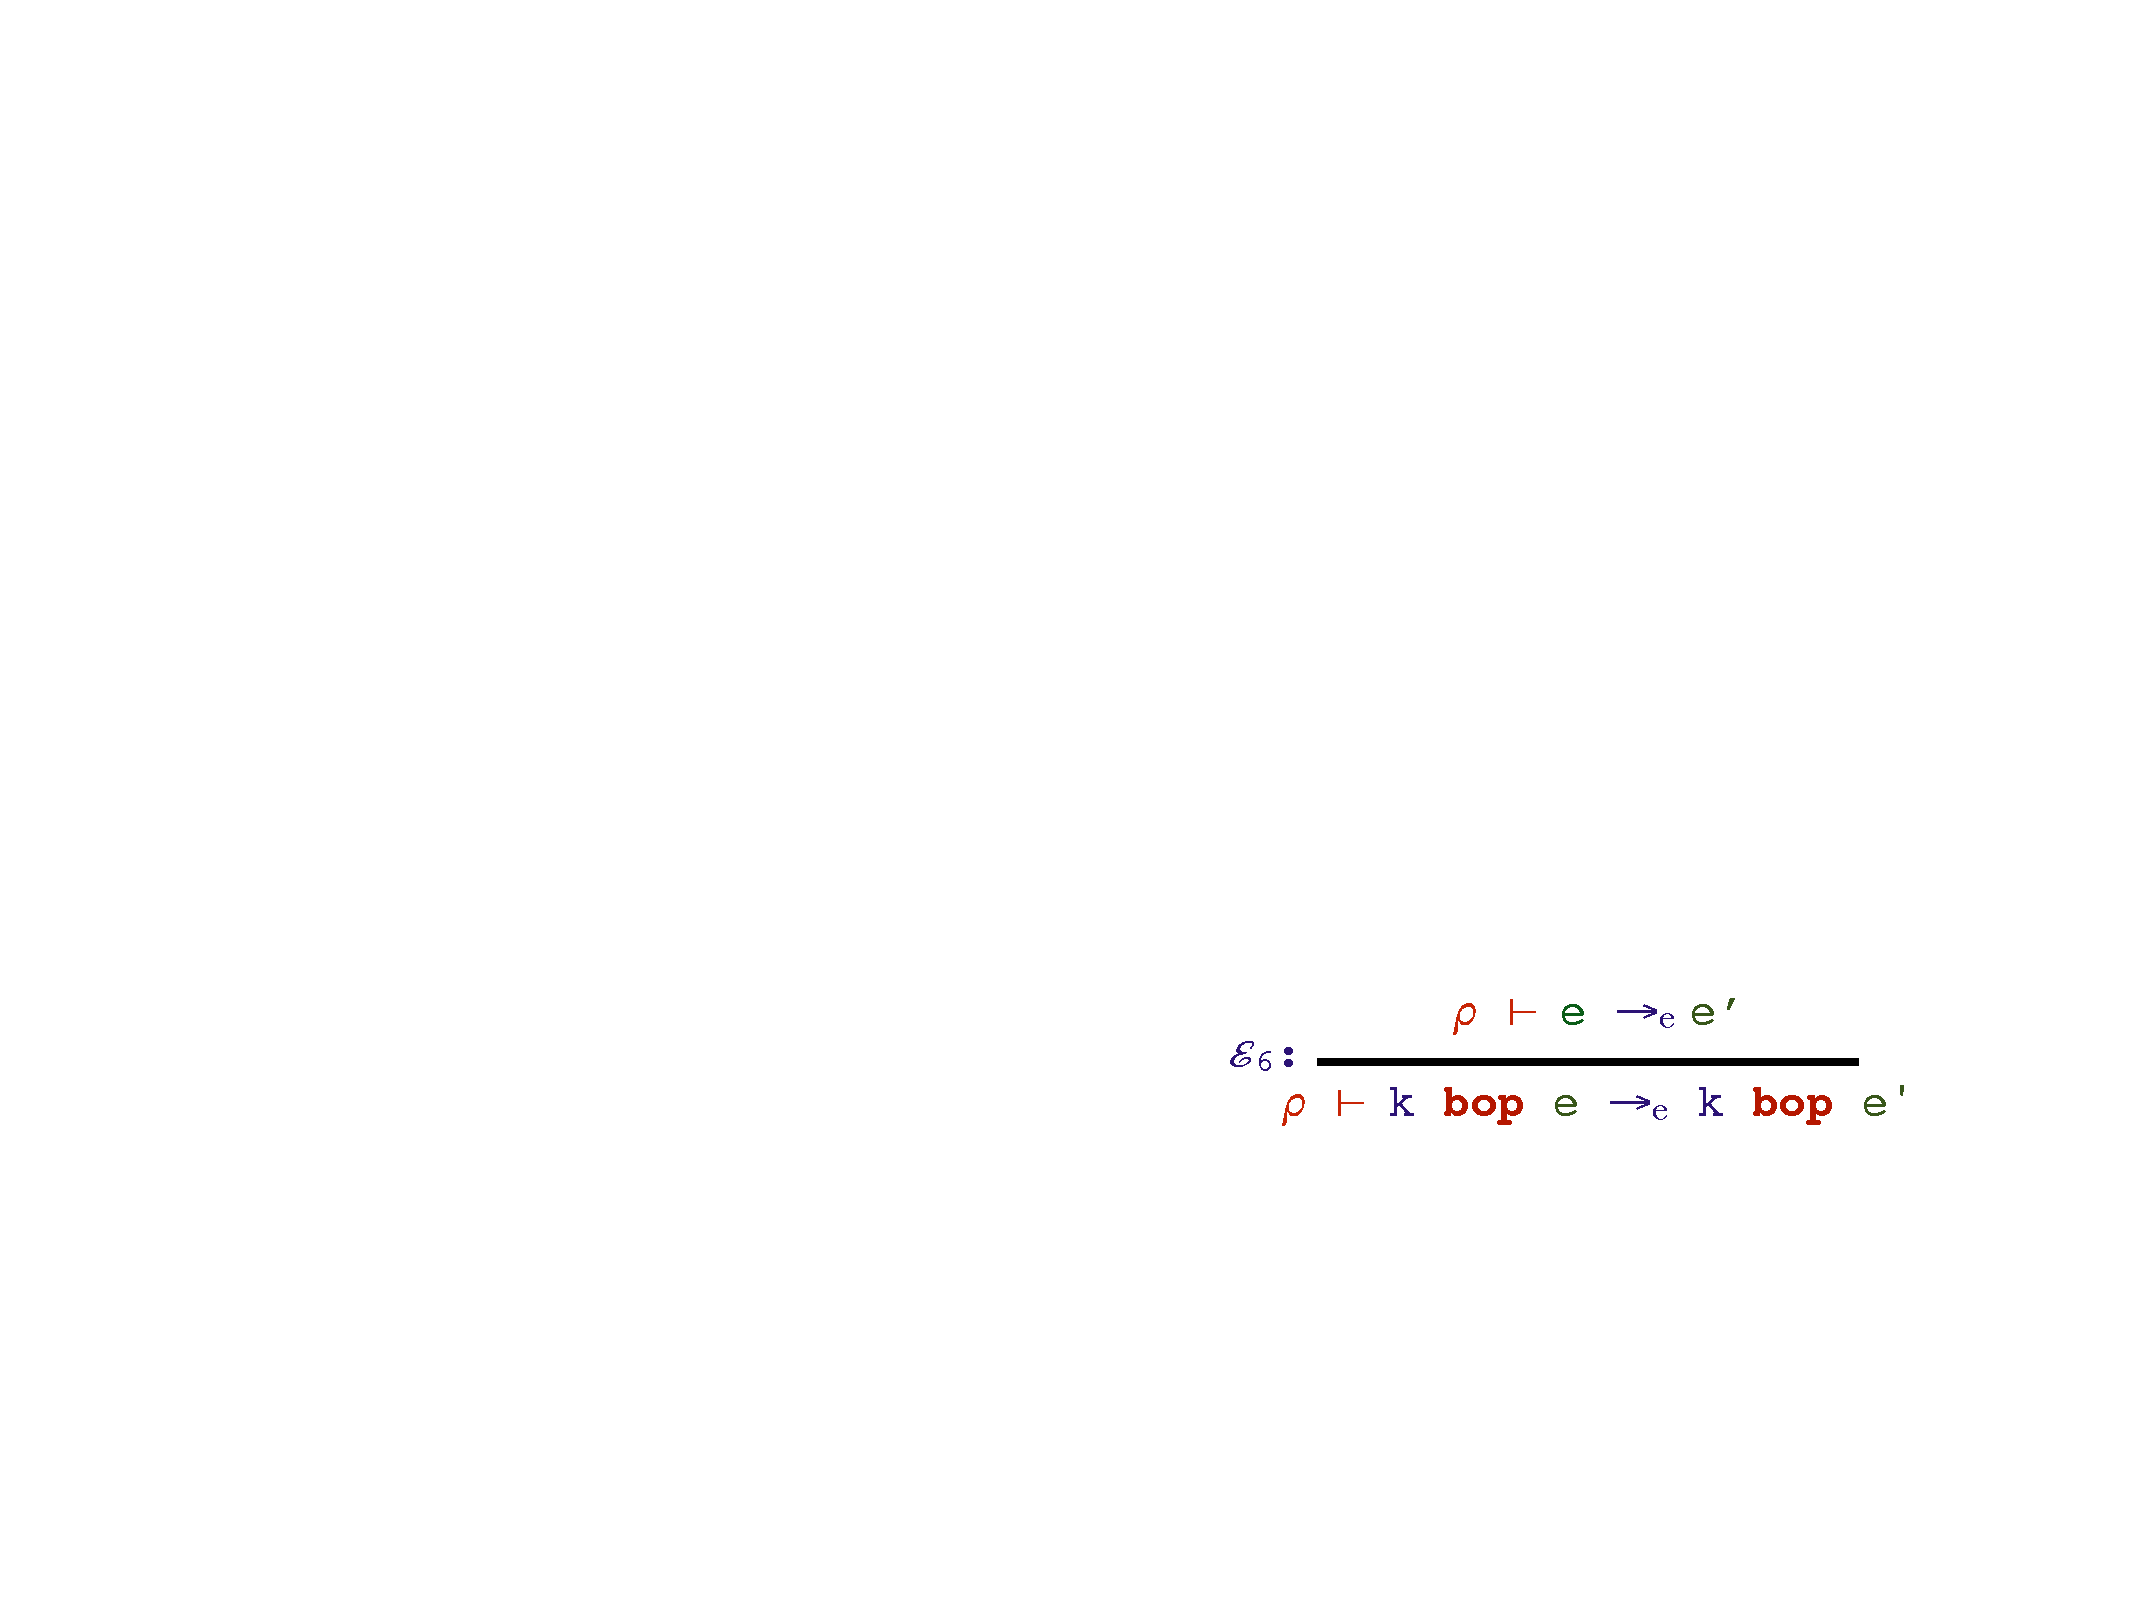
\includegraphics[width=.6\textwidth]{img/regola_espressione-6.pdf}
		\end{figure}
		
		\item La settima regola:
		\begin{figure}[!htp]
			\centering
			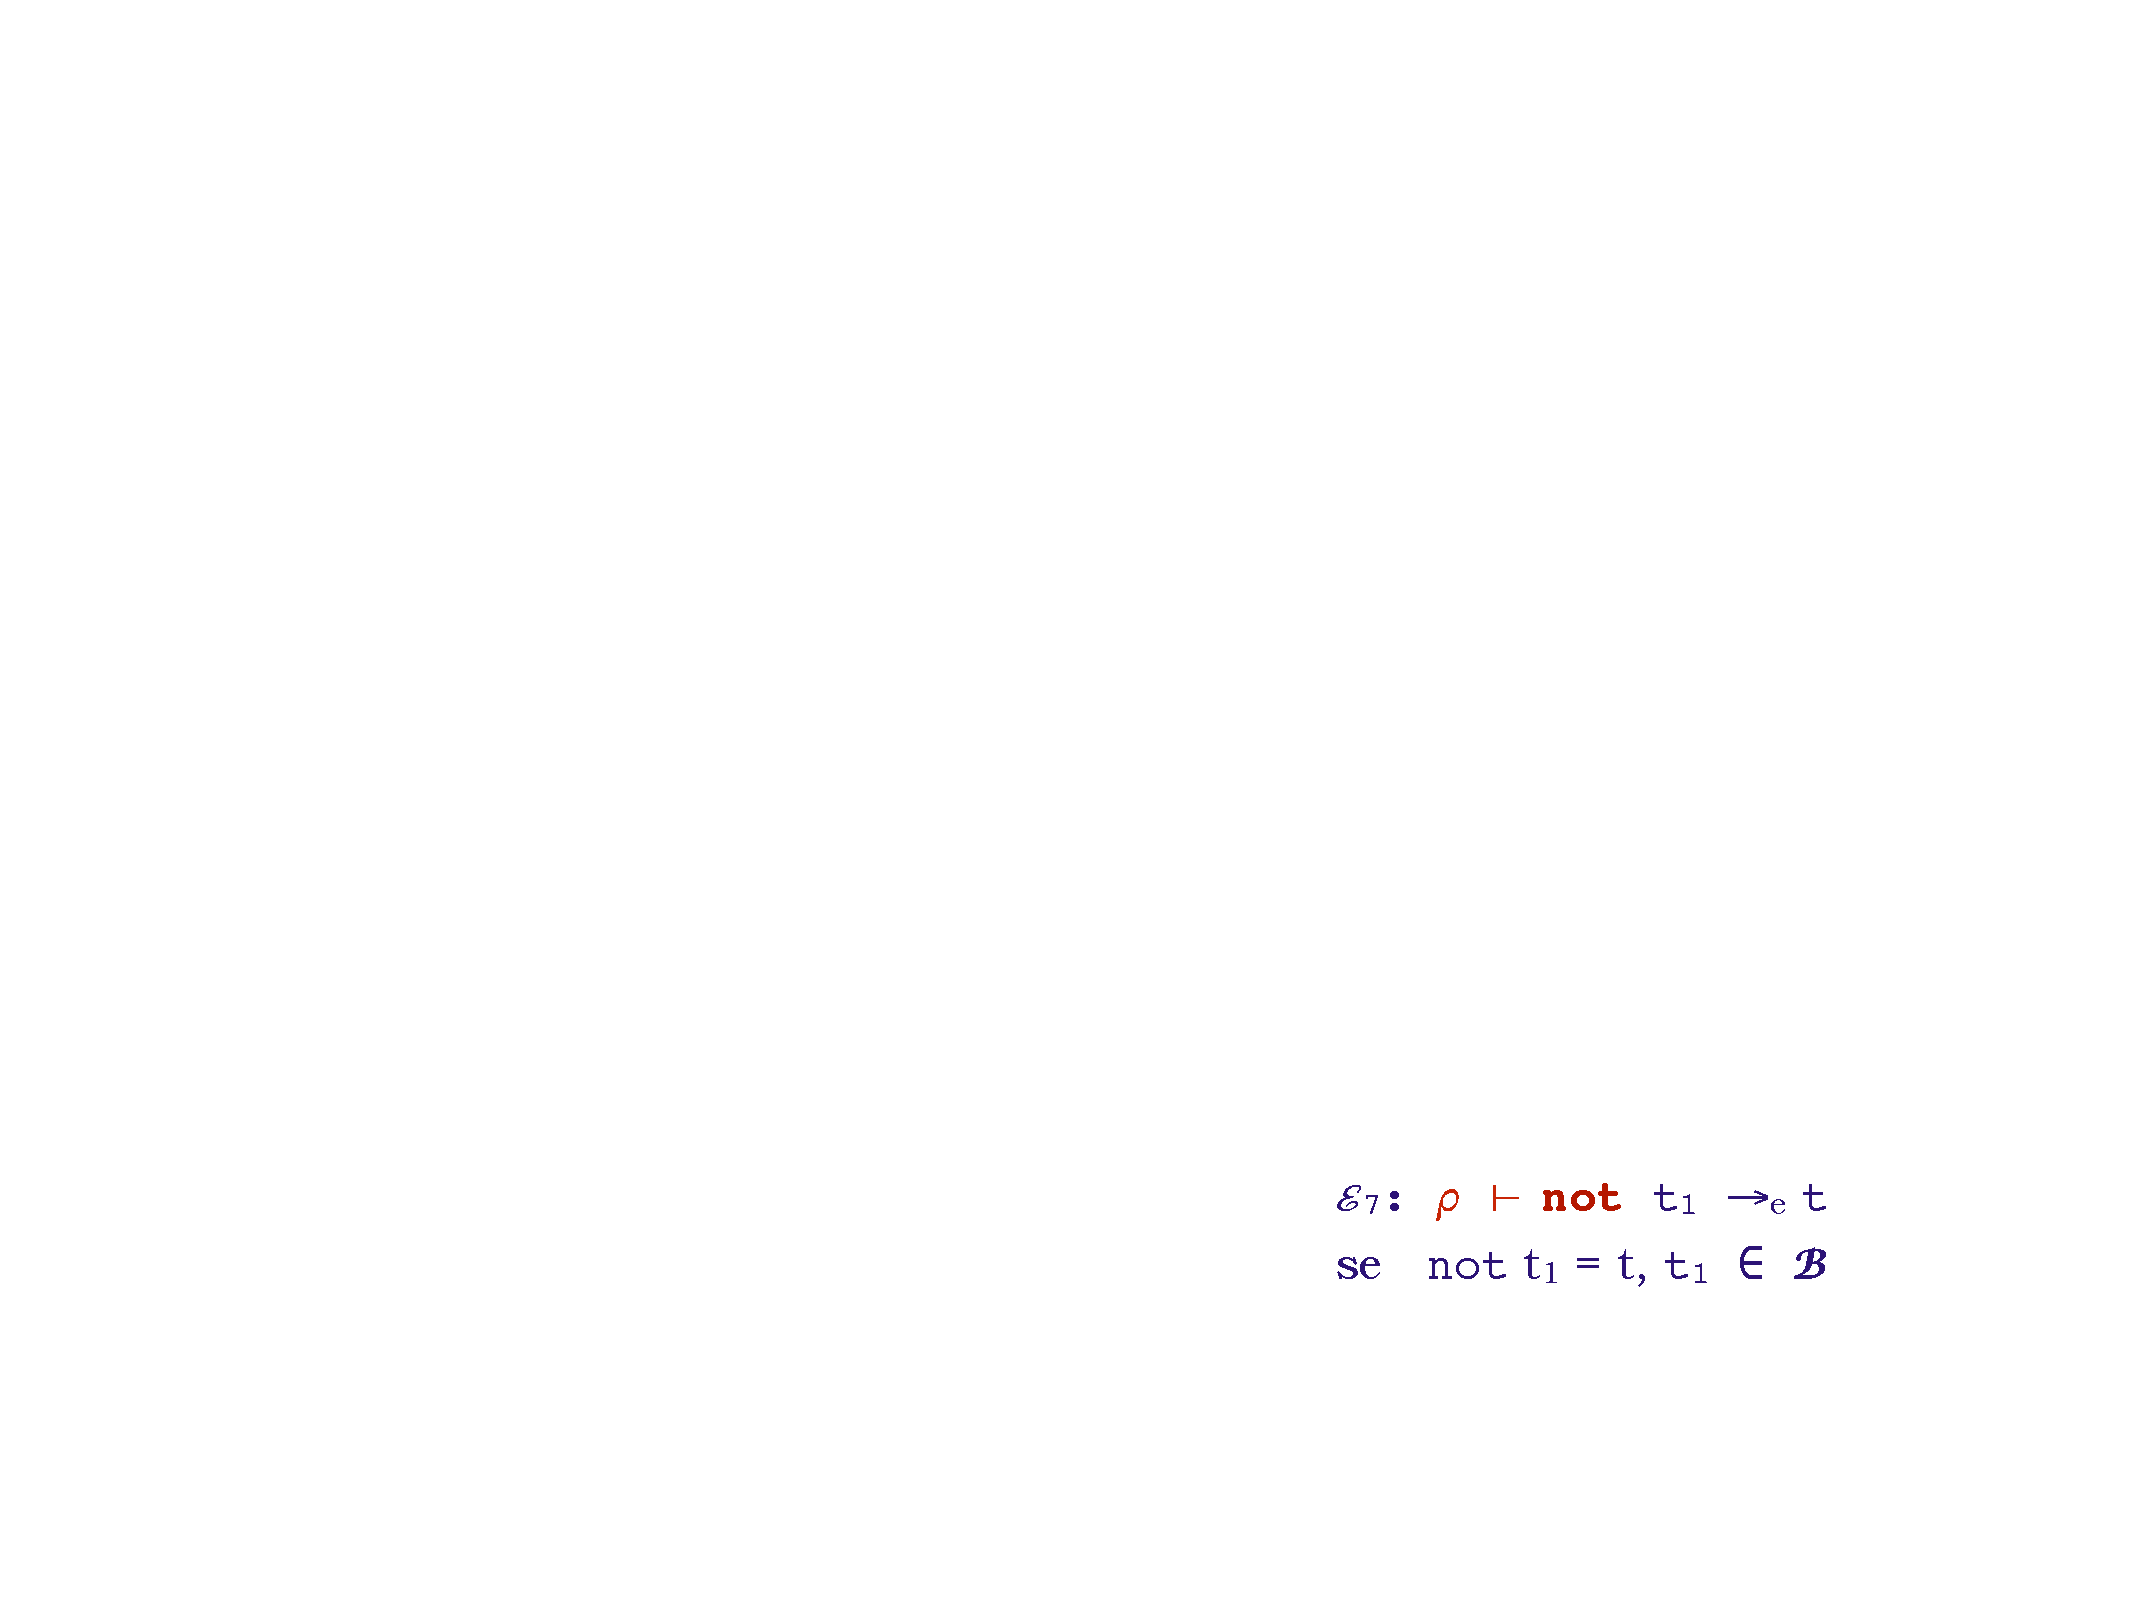
\includegraphics[width=.6\textwidth]{img/regola_espressione-7.pdf}
		\end{figure}
		
		\item L'ottava regola:
		\begin{figure}[!htp]
			\centering
			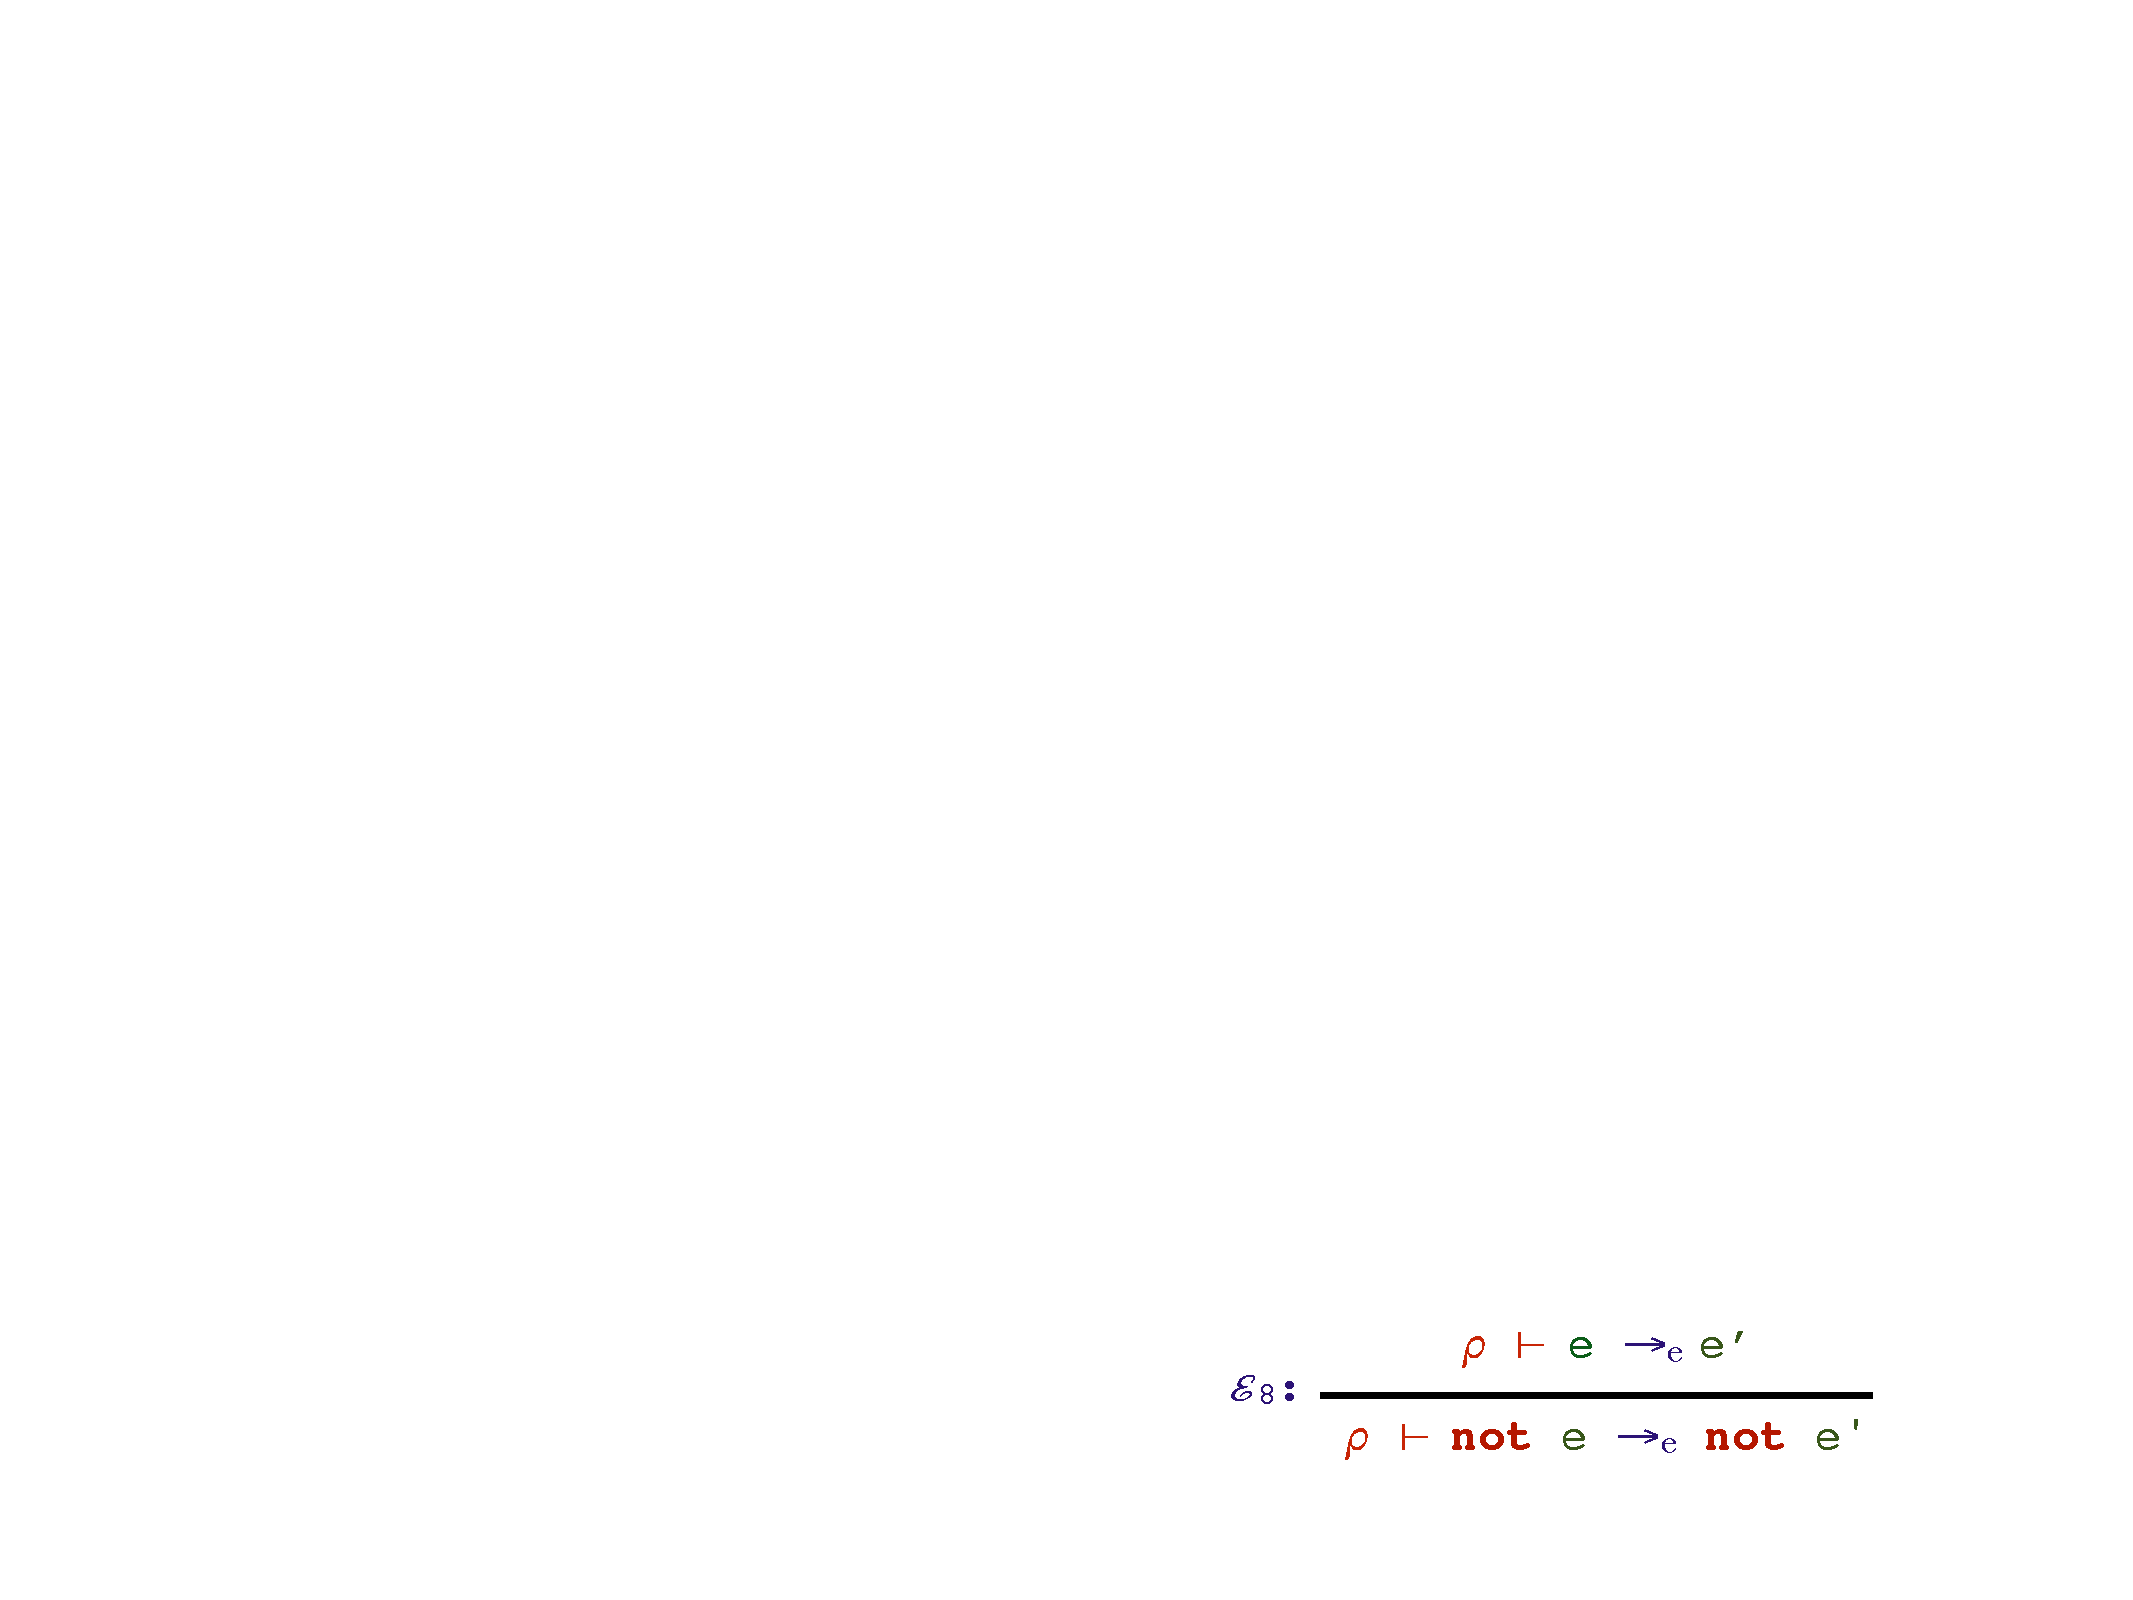
\includegraphics[width=.6\textwidth]{img/regola_espressione-8.pdf}
		\end{figure}
	\end{itemize}\newpage

	
	\subsection{Tipo}
	
	Il \textcolor{Red3}{\textbf{tipo}} \textbf{determina l'insieme di valori dotato di un insieme di operazioni definite per i valori di quel tipo}. In altre parole, il tipo determina il range di valori che un identificatore può memorizzare/denotare e l'insieme di operazioni definite su quei valori.\newline
	
	\noindent
	\textcolor{Green4}{\textbf{Esempi}} di tipo sono:
	\begin{lstlisting}[language=Java]
Integer
String
Int -> Bool
(Int -> Int) -> Bool\end{lstlisting}
	In questo caso, ogni tipo è effettivamente un insieme omogeneo di valori e di operazioni su quei valori.\newline
	
	\noindent
	\textcolor{Green4}{\textbf{Esempi}} di elementi che \underline{non} sono un tipo:
	\begin{lstlisting}[language=Java]
{3, True, \x->x}
Even integers
{f:Int -> Int | x>3 => f(x) > x * (x+1)}\end{lstlisting}\:\newline

	\noindent
	\textbf{La distinzione tra insiemi di valori che sono tipi e insiemi che non lo sono \emph{dipende dal linguaggio}}. Inoltre, i tipi sono \textbf{utili a vari livelli}:
	\begin{itemize}
		\item \textbf{Livello di progetto:} organizzano l'informazione, come i commenti;
		
		\item \textbf{Livello di programma:} identificano e prevengono errori. Per esempio $3+"stringa"$ deve essere sbagliato;
		
		\item \textbf{Livello di implementazione:} consentono alcune ottimizzazioni, per esempio il tipo $Bool$ richiede meno bit di $real$.
	\end{itemize}

	\longline
	
	\subsubsection{Binding di tipo (\emph{Type binding})}
	
	A seconda del legame, esistono due tipi di dichiarazione:
	\begin{itemize}
		\item Legame \textbf{statico}: quando il \textbf{legame, una volta creato, rimane inalterato per l'intera esecuzione}. Esistono due tipi di dichiarazione per specificare questo legame:
		\begin{itemize}
			\item \textcolor{Red3}{\textbf{Esplicita}}: quando esiste un comando del linguaggio che consente di \textbf{dichiarare il tipo delle variabili};
			
			\item \textcolor{Red3}{\textbf{Implicita}}: è un meccanismo di default che specifica il \textbf{tipo delle variabili attraverso convenzioni} di default (maggiore facilità di scrittura, ma scarsa affidabilità).
		\end{itemize}
		
		\item Legame \textbf{dinamico}: quando il \textbf{legame può cambiare durante l'esecuzione}. Per esempio in Python è possibile dichiarare una variabile senza esplicitare il tipo. Questo porta un \textcolor{Green4}{\textbf{vantaggio}} in termini di flessibilità, ma \textcolor{Red3}{\textbf{svantaggi}} in termini di costi di implementazione (alti) e una difficile rilevazione di errori di tipo.
	\end{itemize}
	
	\subsection{Ambiente statico e semantica statica}
	
	L'\textbf{ambiente statico} associa agli identificatori il tipo degli oggetti che denoteranno.
	\begin{boxdef}
		Un \textcolor{Red3}{\textbf{ambiente statico}} (o di tipi) è un elemento dello spazio di funzioni $TEnv$ definito da:
		\begin{equation*}
			TEnv = \cup_{V \subseteq_{f} Id} TEnv_{V}
		\end{equation*}
		Dove:
		\begin{equation*}
			TEnv_{V} : V \rightarrow DTyp \hspace{2em} \text{ ha metavariabile }
		\end{equation*}
		E $DTyp$ è l'insieme dei tipi denotabili.
	\end{boxdef}

	\noindent
	Per il momento $DTyp$ sono solo interi e booleani.\newline
	
	\noindent
	Si considera anche un elemento speciale che rappresenta il \textbf{tipo di un identificatore non inizializzato}:
	\begin{equation*}
		\tau \in DTyp = \left\{\textsf{int}, \textsf{bool}, \bot\right\}
	\end{equation*}
	Quindi, la semantica statica è un \textbf{insieme di regole che consentono di associare un tipo ad ogni espressione corretta}; in questo caso l'espressione viene detta \textcolor{Red3}{\textbf{ben formata}}. Inoltre, le regole della semantica statica hanno la seguente forma:\label{ben formata}
	\begin{figure}[!htp]
		\centering
		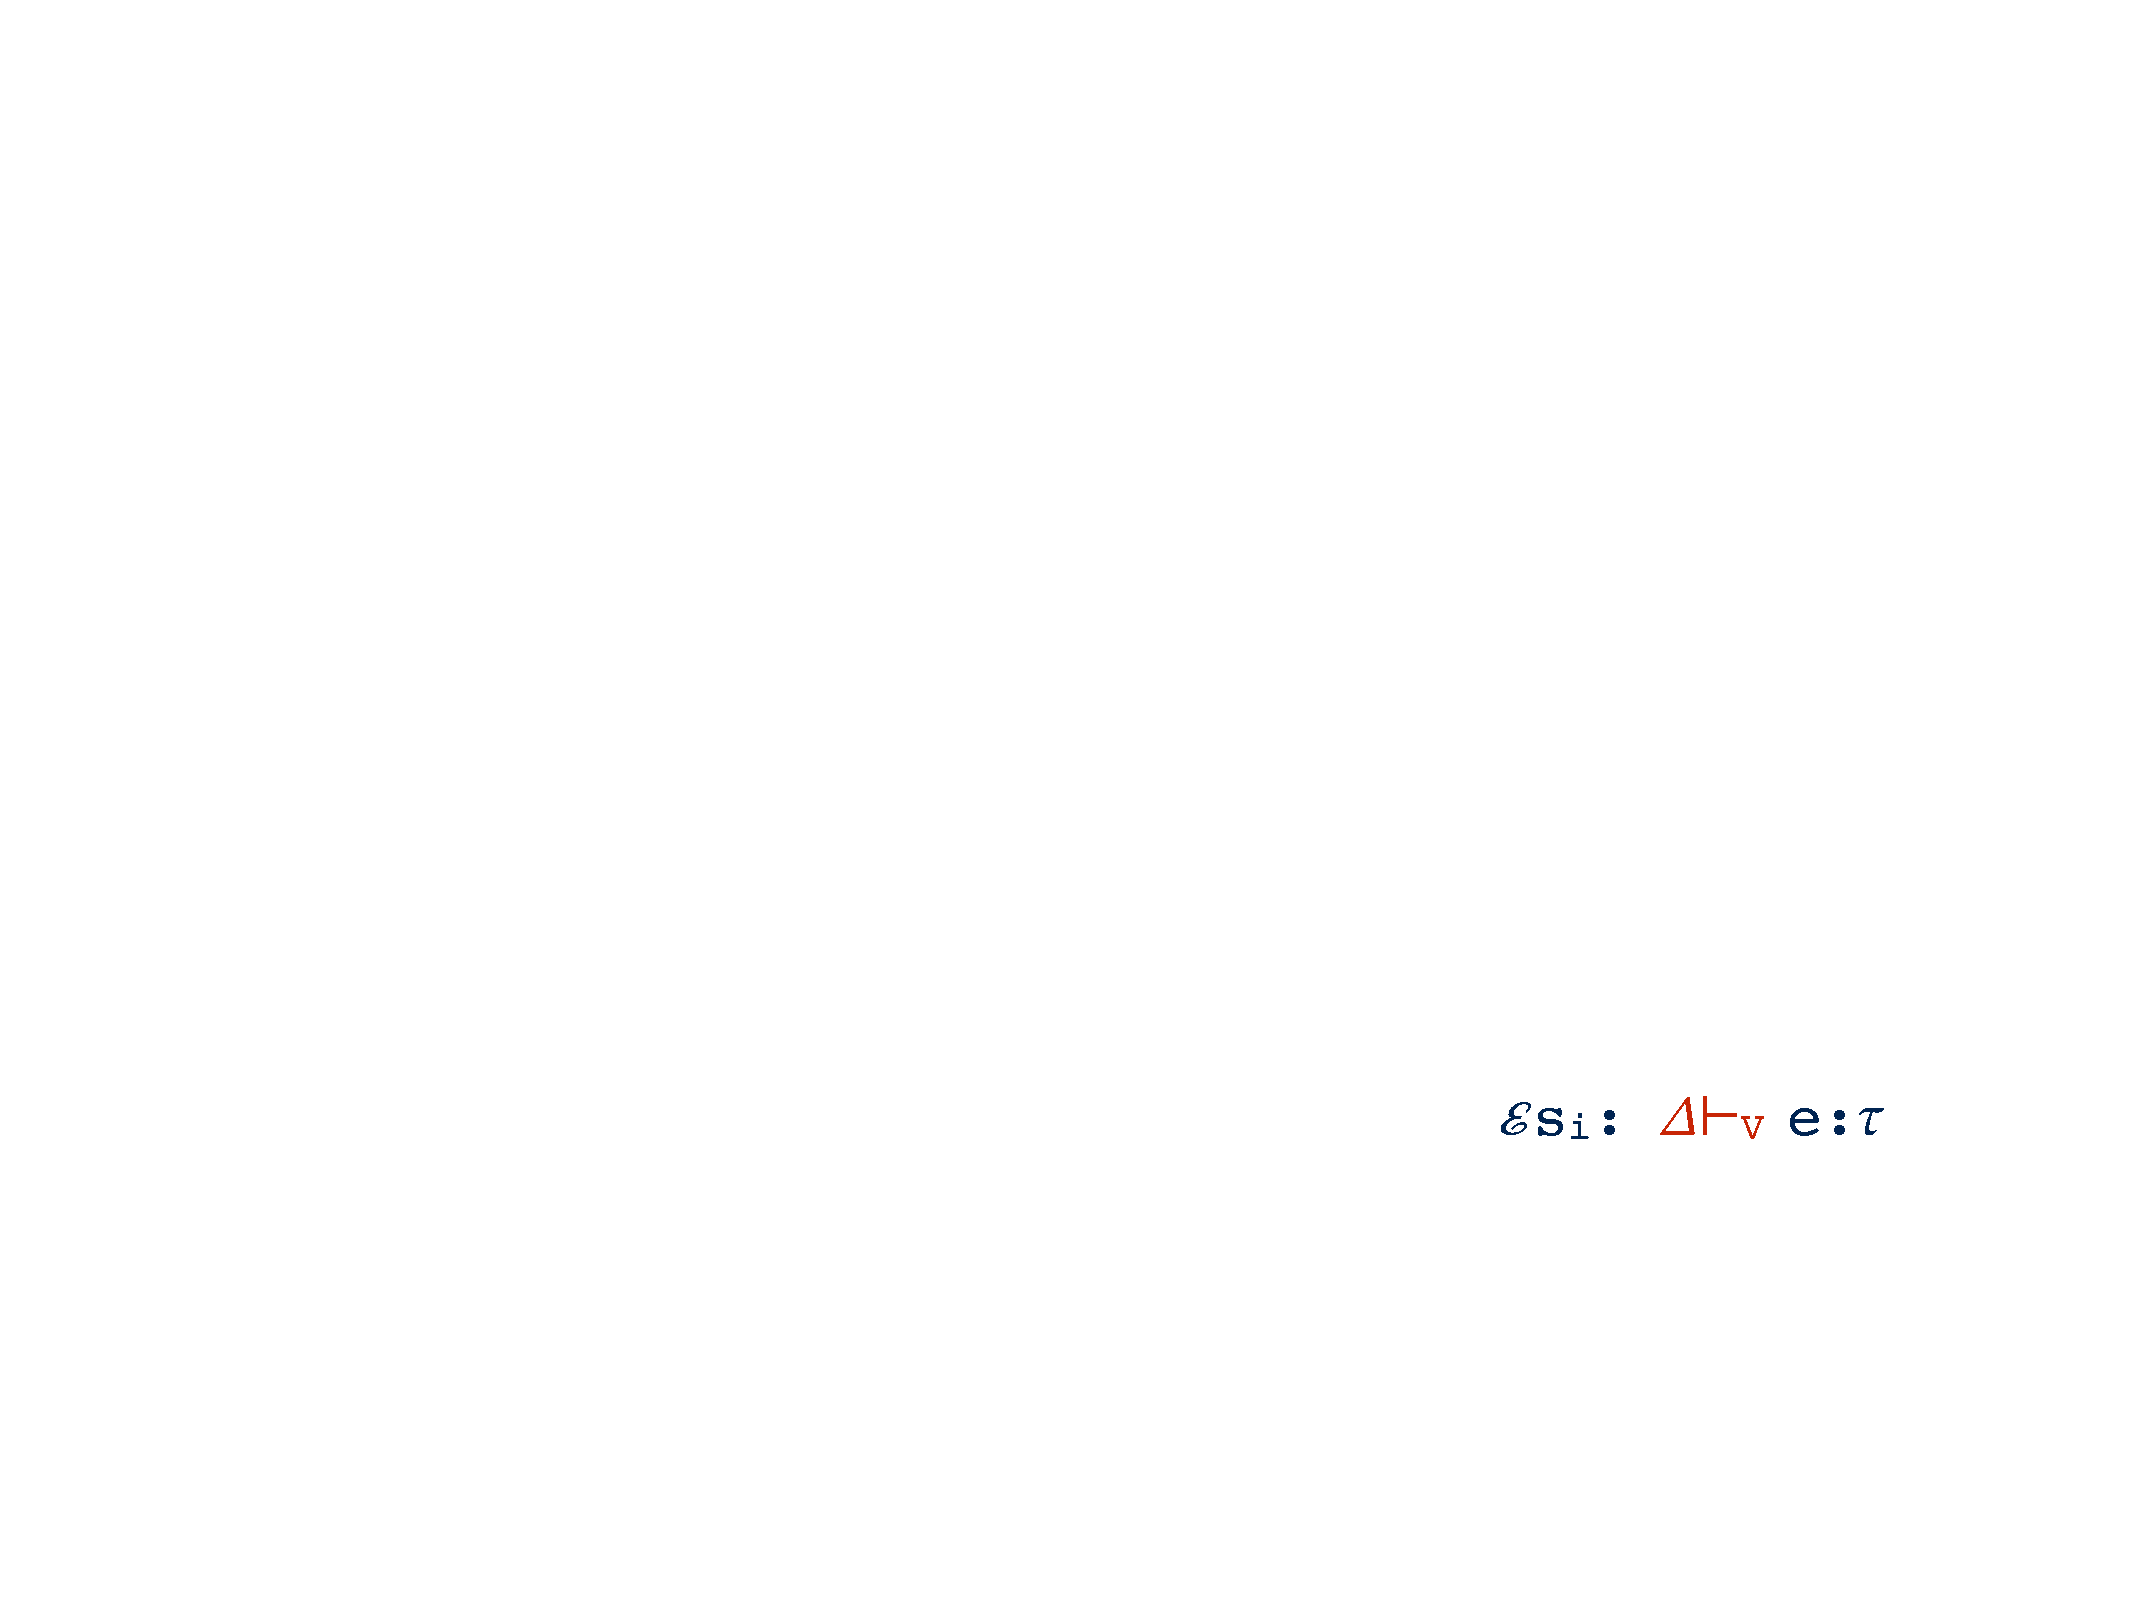
\includegraphics[width=.3\textwidth]{img/semantica_statica.pdf}
	\end{figure}
	
	\noindent
	\begin{itemize}
		\item $\Delta$ indica l'\textbf{ambiente statico} nel quale valutare staticamente l'espressione, ovvero l'insieme dei legami statici validi nel contesto di valutazione.
		
		\item $V$ indica l'\textbf{insieme degli identificatori} per i quali l'ambiente definisce un'associazione.
	\end{itemize}
	Nel caso in cui questi elementi non sono presenti, significa che l'ambiente è vuoto. In tal caso, si dice che $e$ è di tipo $\tau$ nell'ambiente $\Delta$.\newpage

	\subsubsection{Semantica statica delle espressioni}
	
	Si introducono le \textcolor{Red3}{\textbf{regole della semantica statica delle espressioni}}. Le prime tre regole sono assiomi, mentre le restanti riguardano operazioni booleane e aritmetiche. Esse vengono definite usando delle funzioni che determinano il tipo del risultato di un operatore booleano o aritmetico in funzione del tipo degli operandi:
	\begin{itemize}
		\item La prima regola è un \textbf{assioma} e dice che nell'ambiente vuoto, cioè qualsiasi, un numero ha tipo intero (int):
		\begin{figure}[!htp]
			\centering
			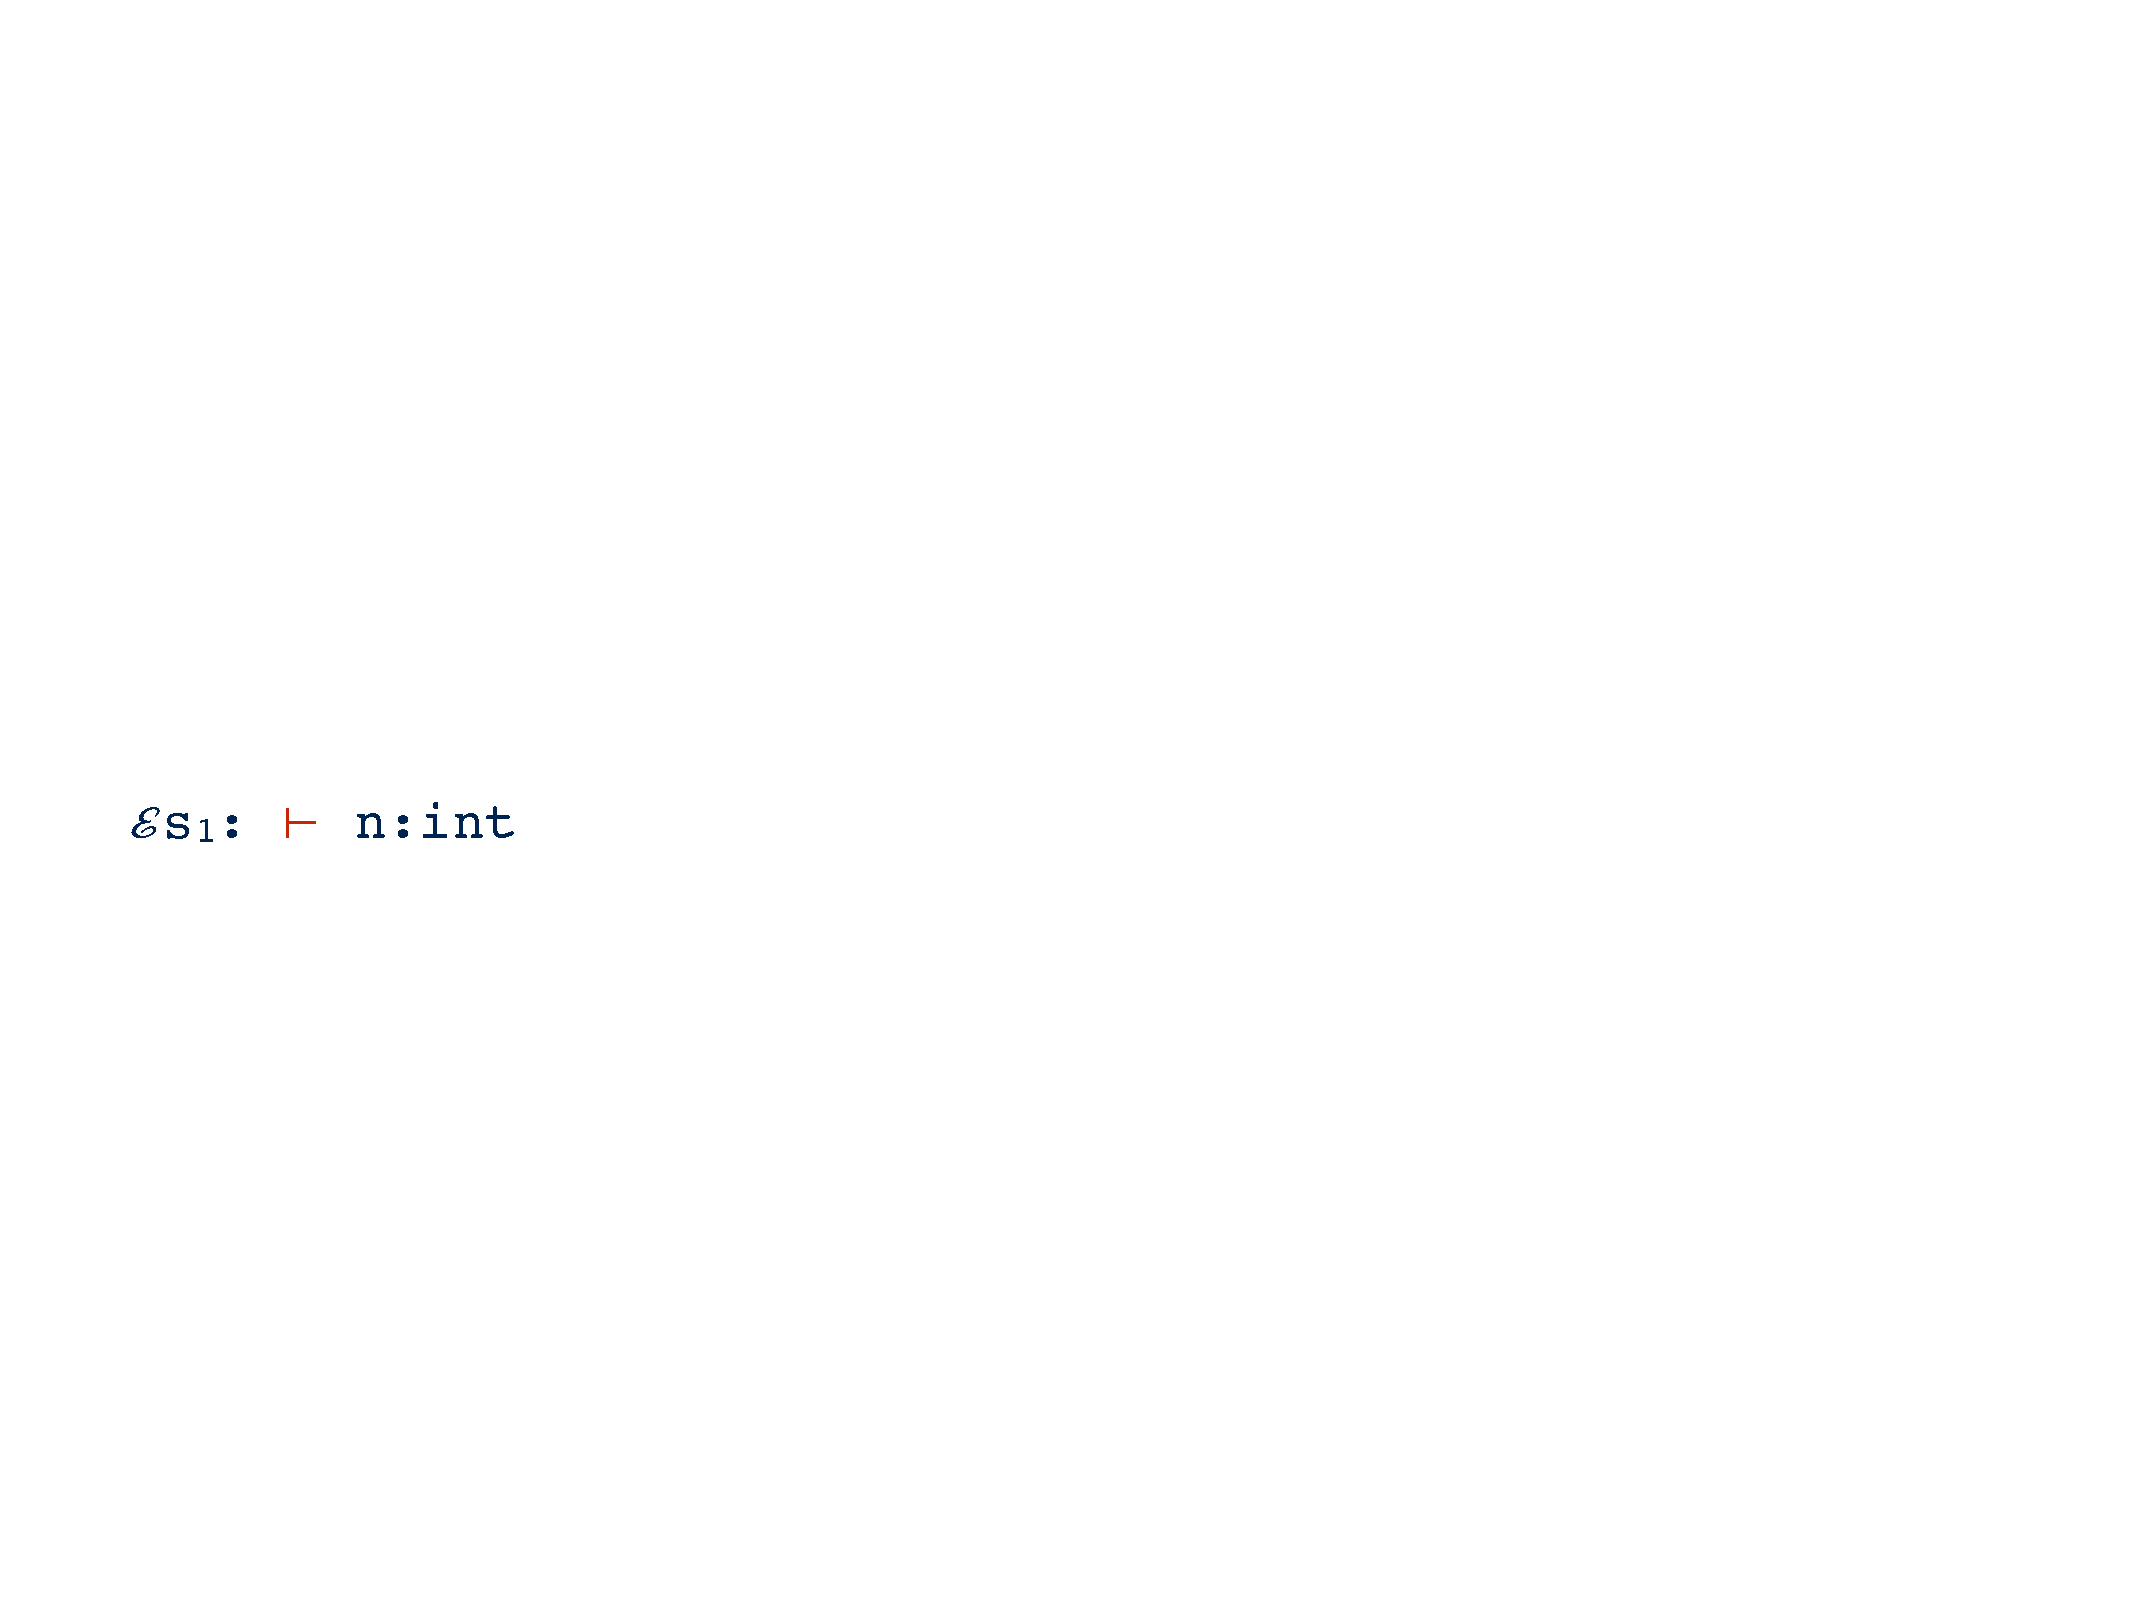
\includegraphics[width=.3\textwidth]{img/regola_semantica-1.pdf}
		\end{figure}
	
		\item La seconda regola è un \textbf{assioma} e dice che nell'ambiente vuoto, cioè qualsiasi, una costante booleana ha tipo booleano (bool):
		\begin{figure}[!htp]
			\centering
			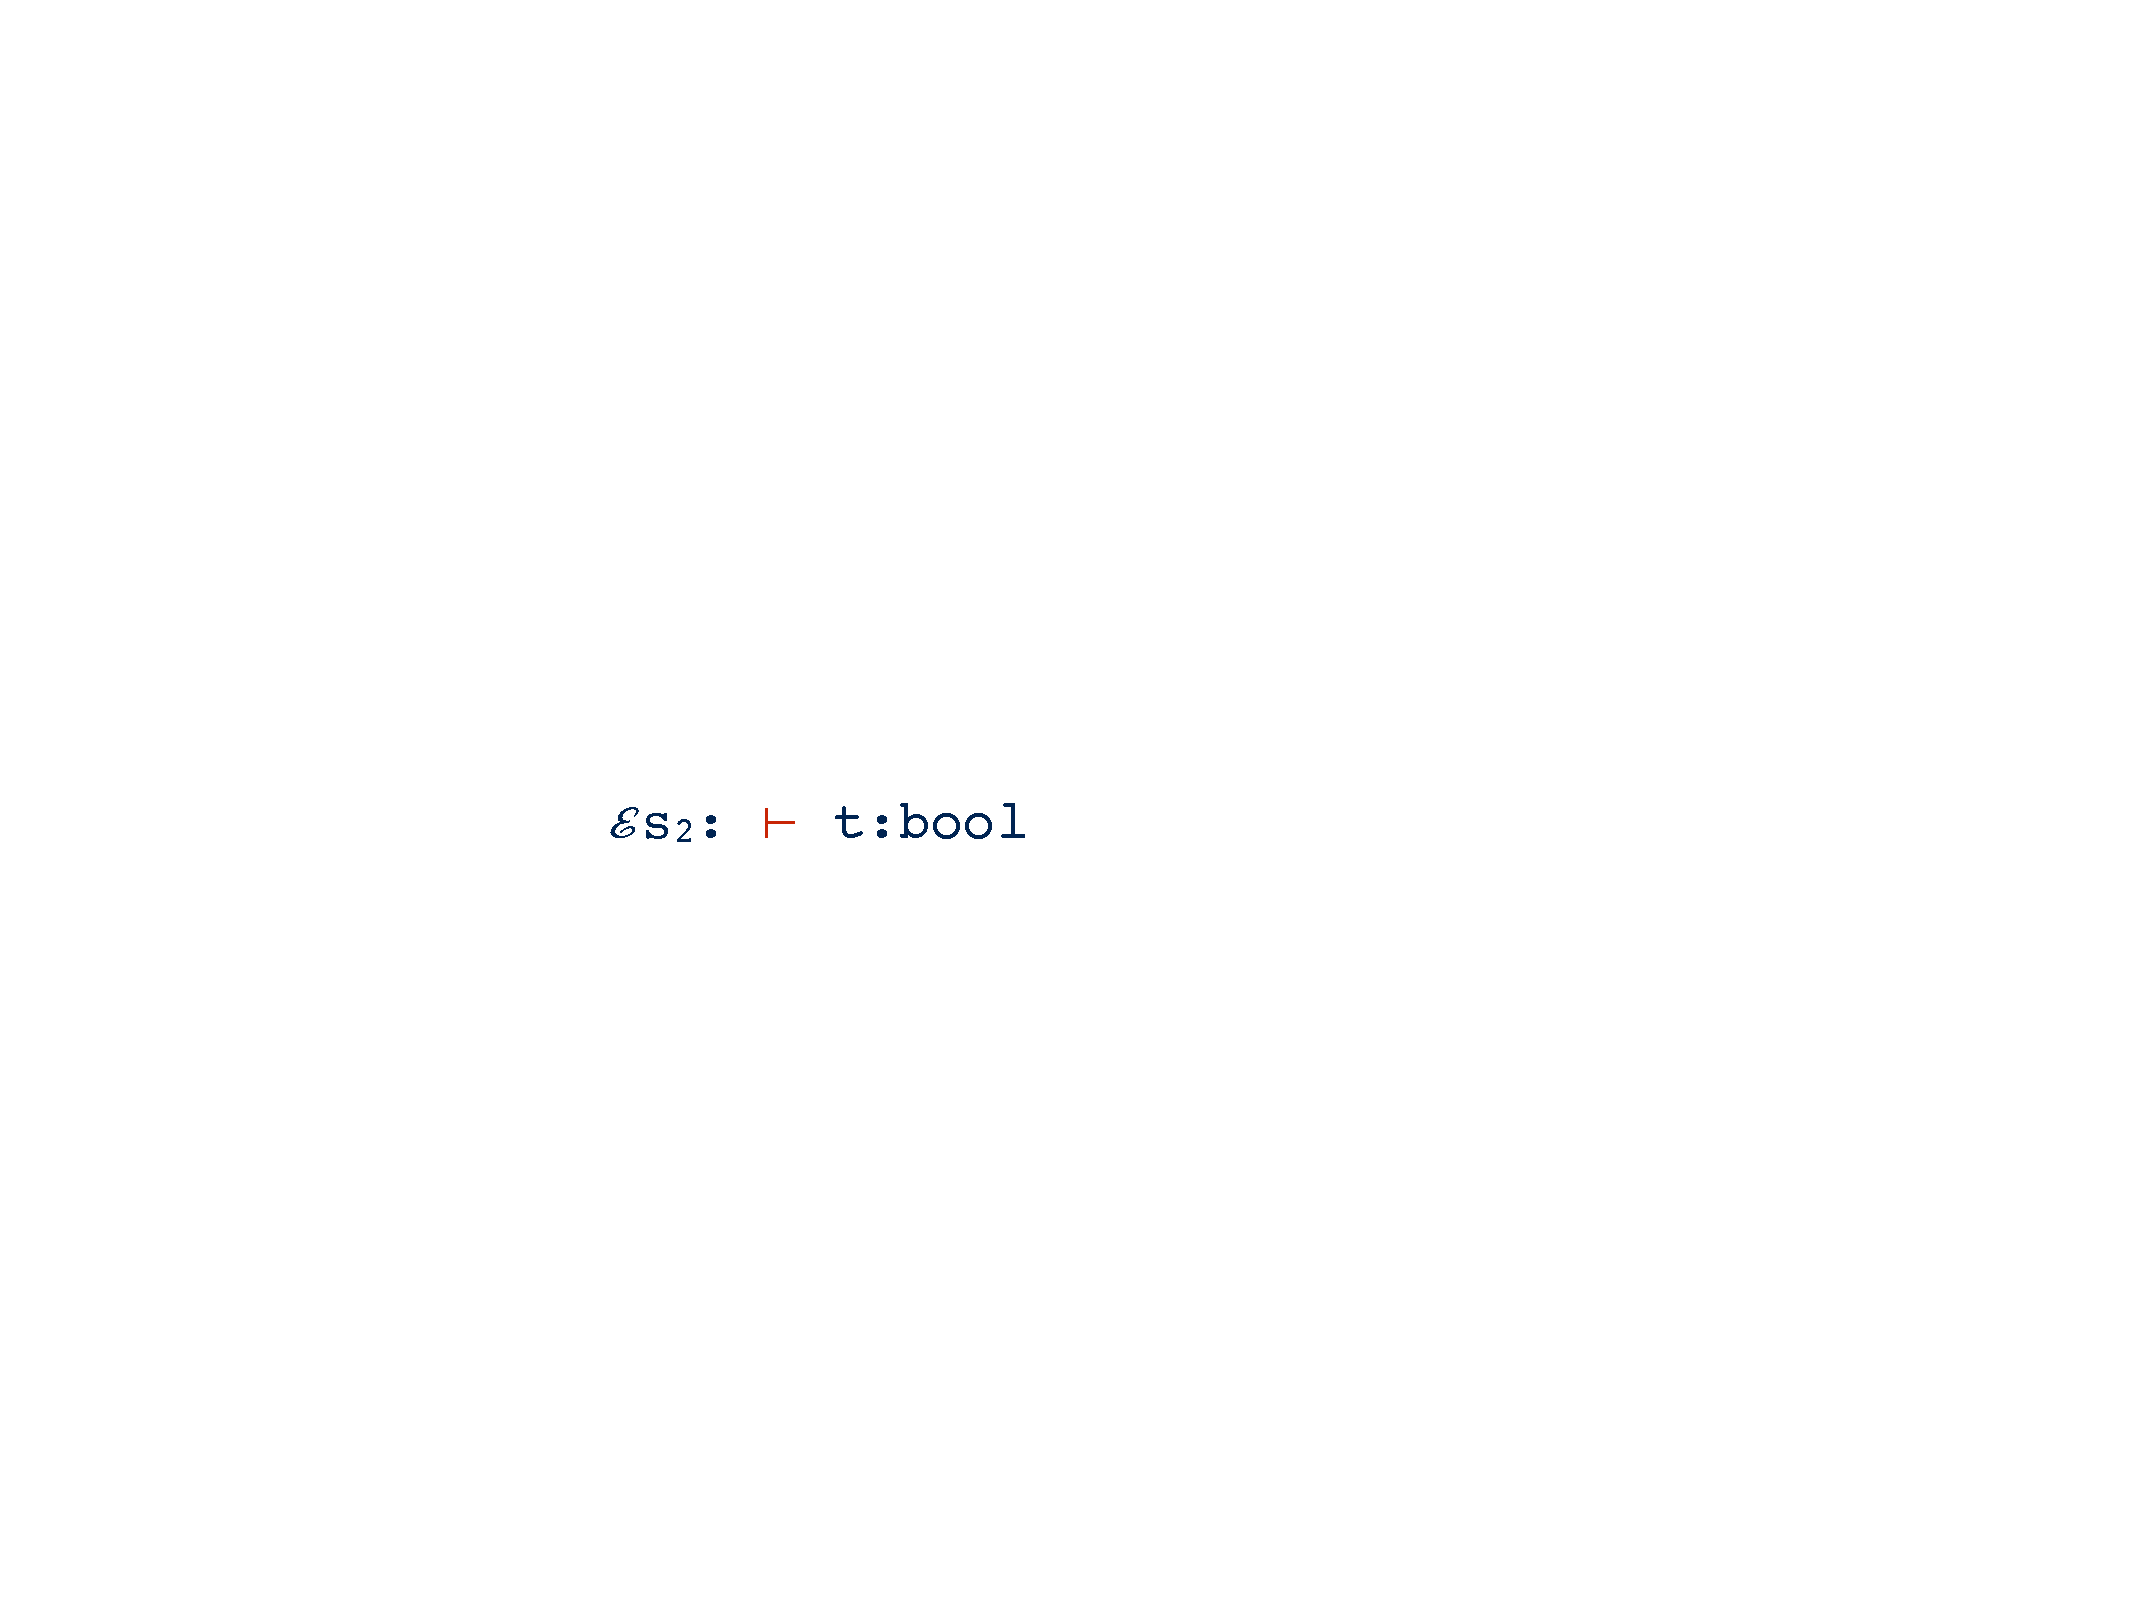
\includegraphics[width=.3\textwidth]{img/regola_semantica-2.pdf}
		\end{figure}
	
		\item La terza regola è un \textbf{assioma} e riguarda gli identificatori. In questo caso, la regola determina che l'identificatore ha come tipo proprio quello che l'ambiente statico $\delta$ del contesto gli associa:
		\begin{figure}[!htp]
			\centering
			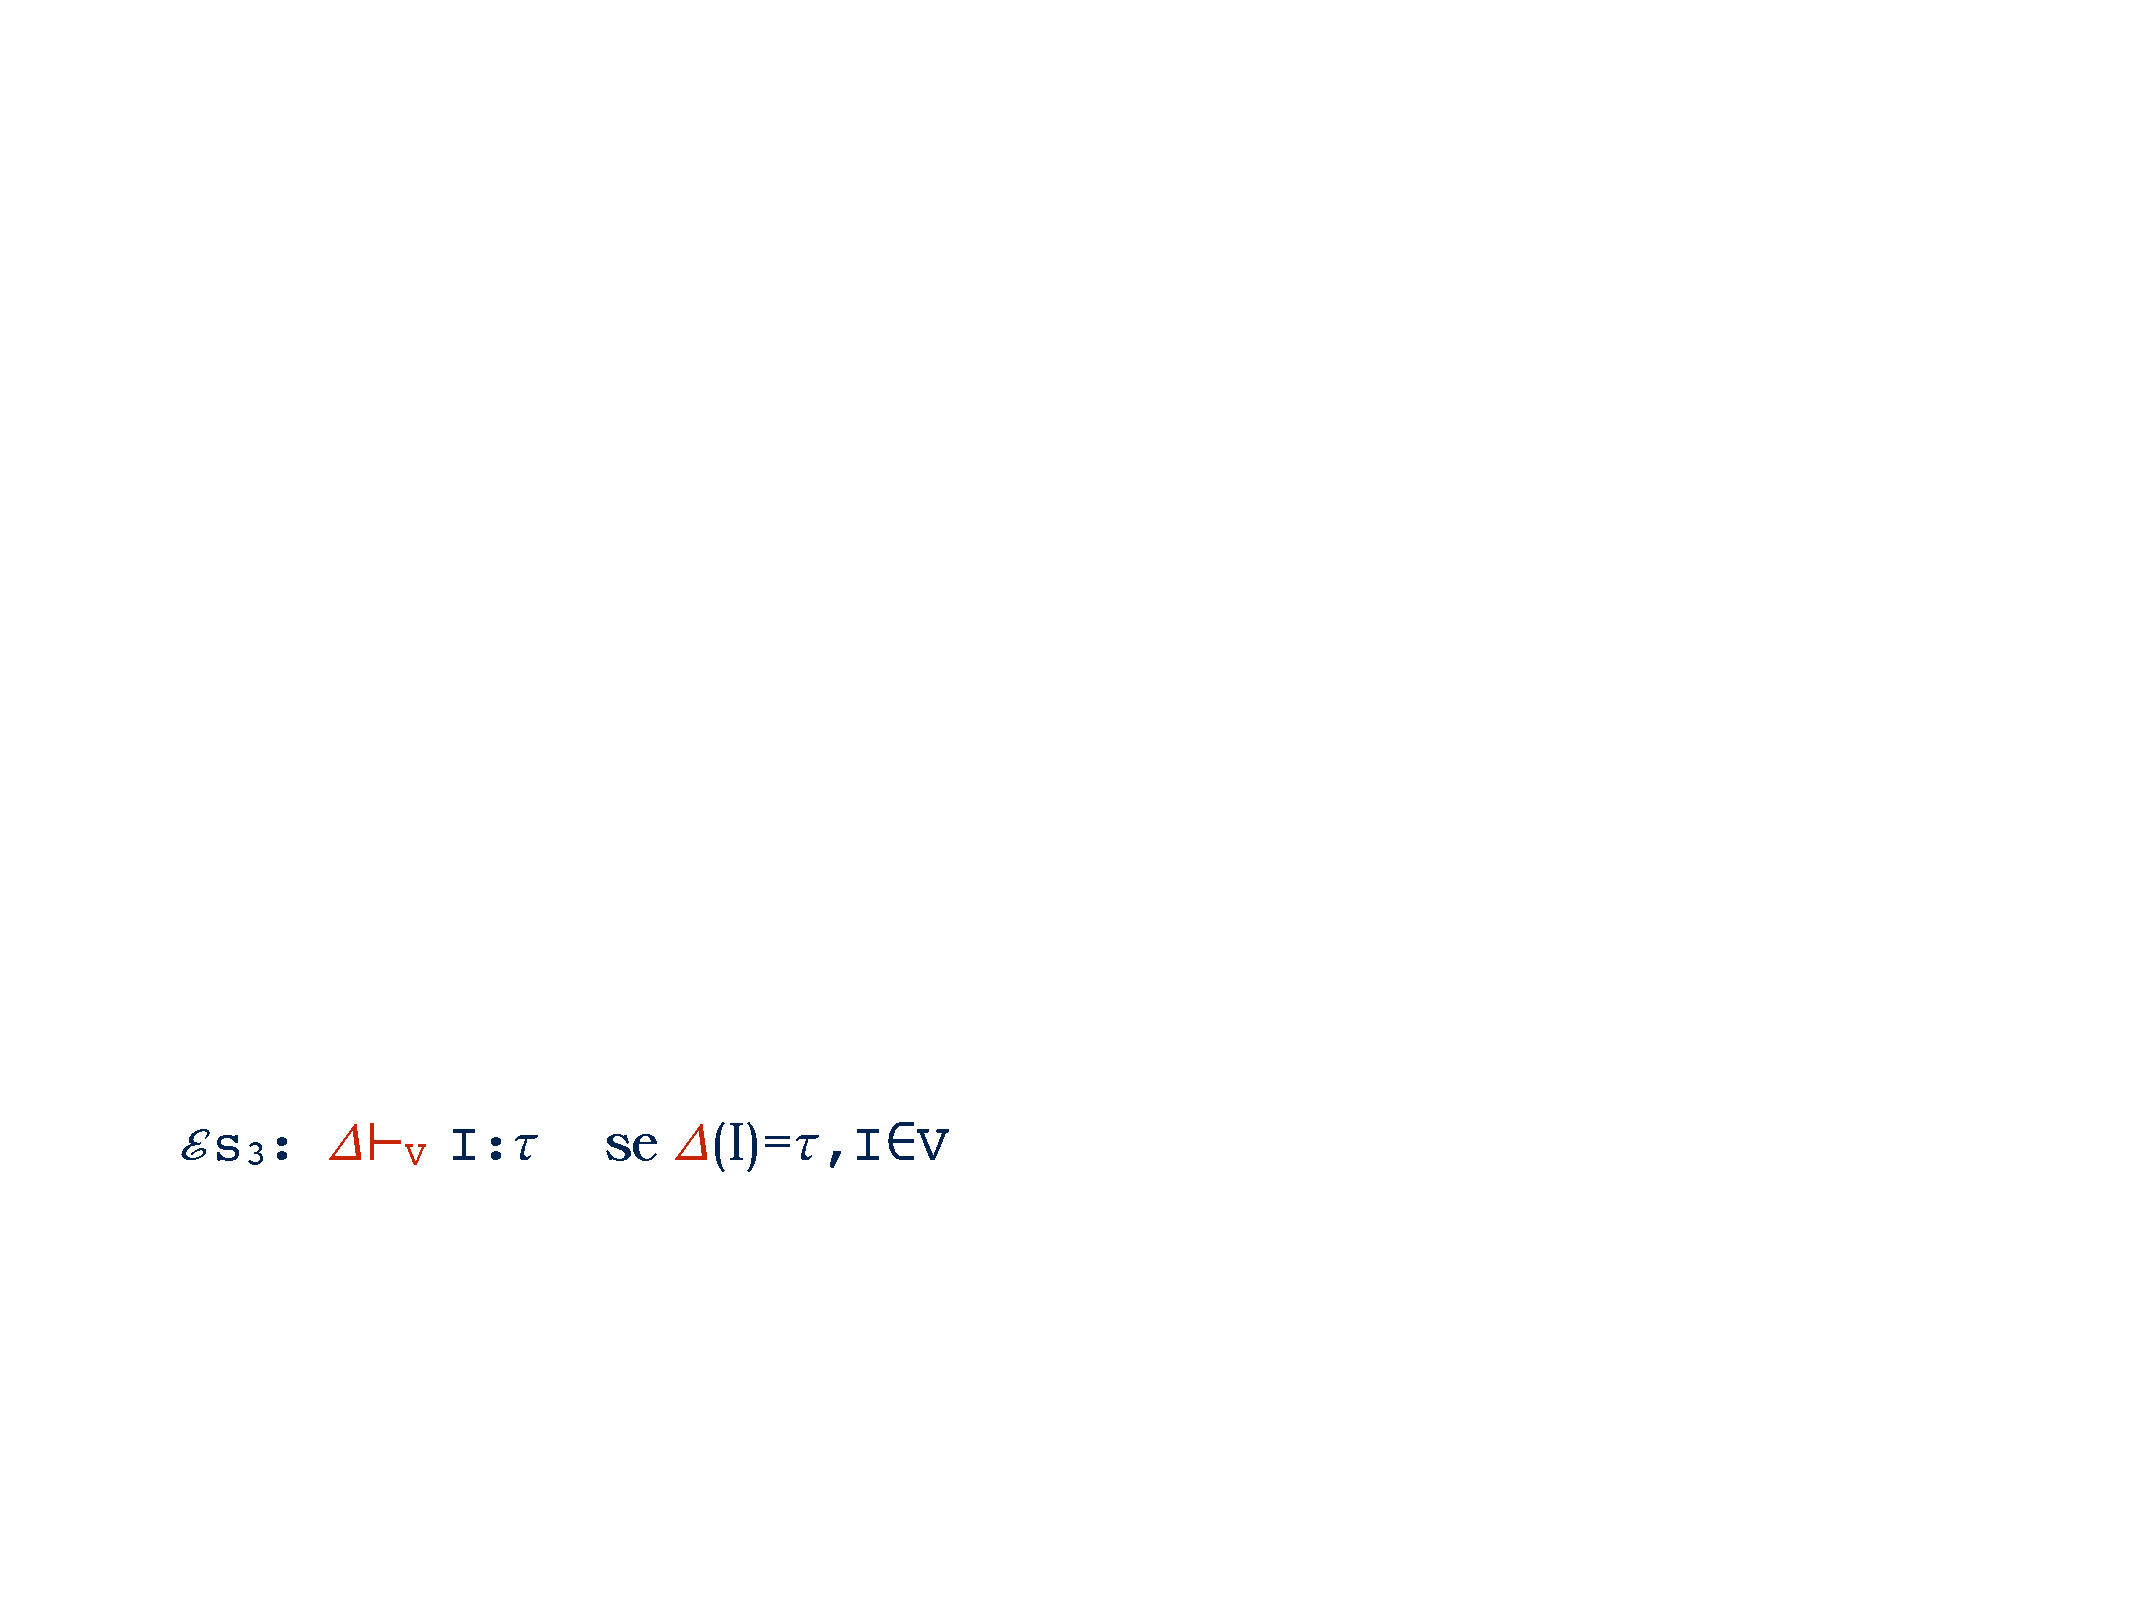
\includegraphics[width=.6\textwidth]{img/regola_semantica-3.pdf}
		\end{figure}
	
		\item La quarta regola:
		\begin{figure}[!htp]
			\centering
			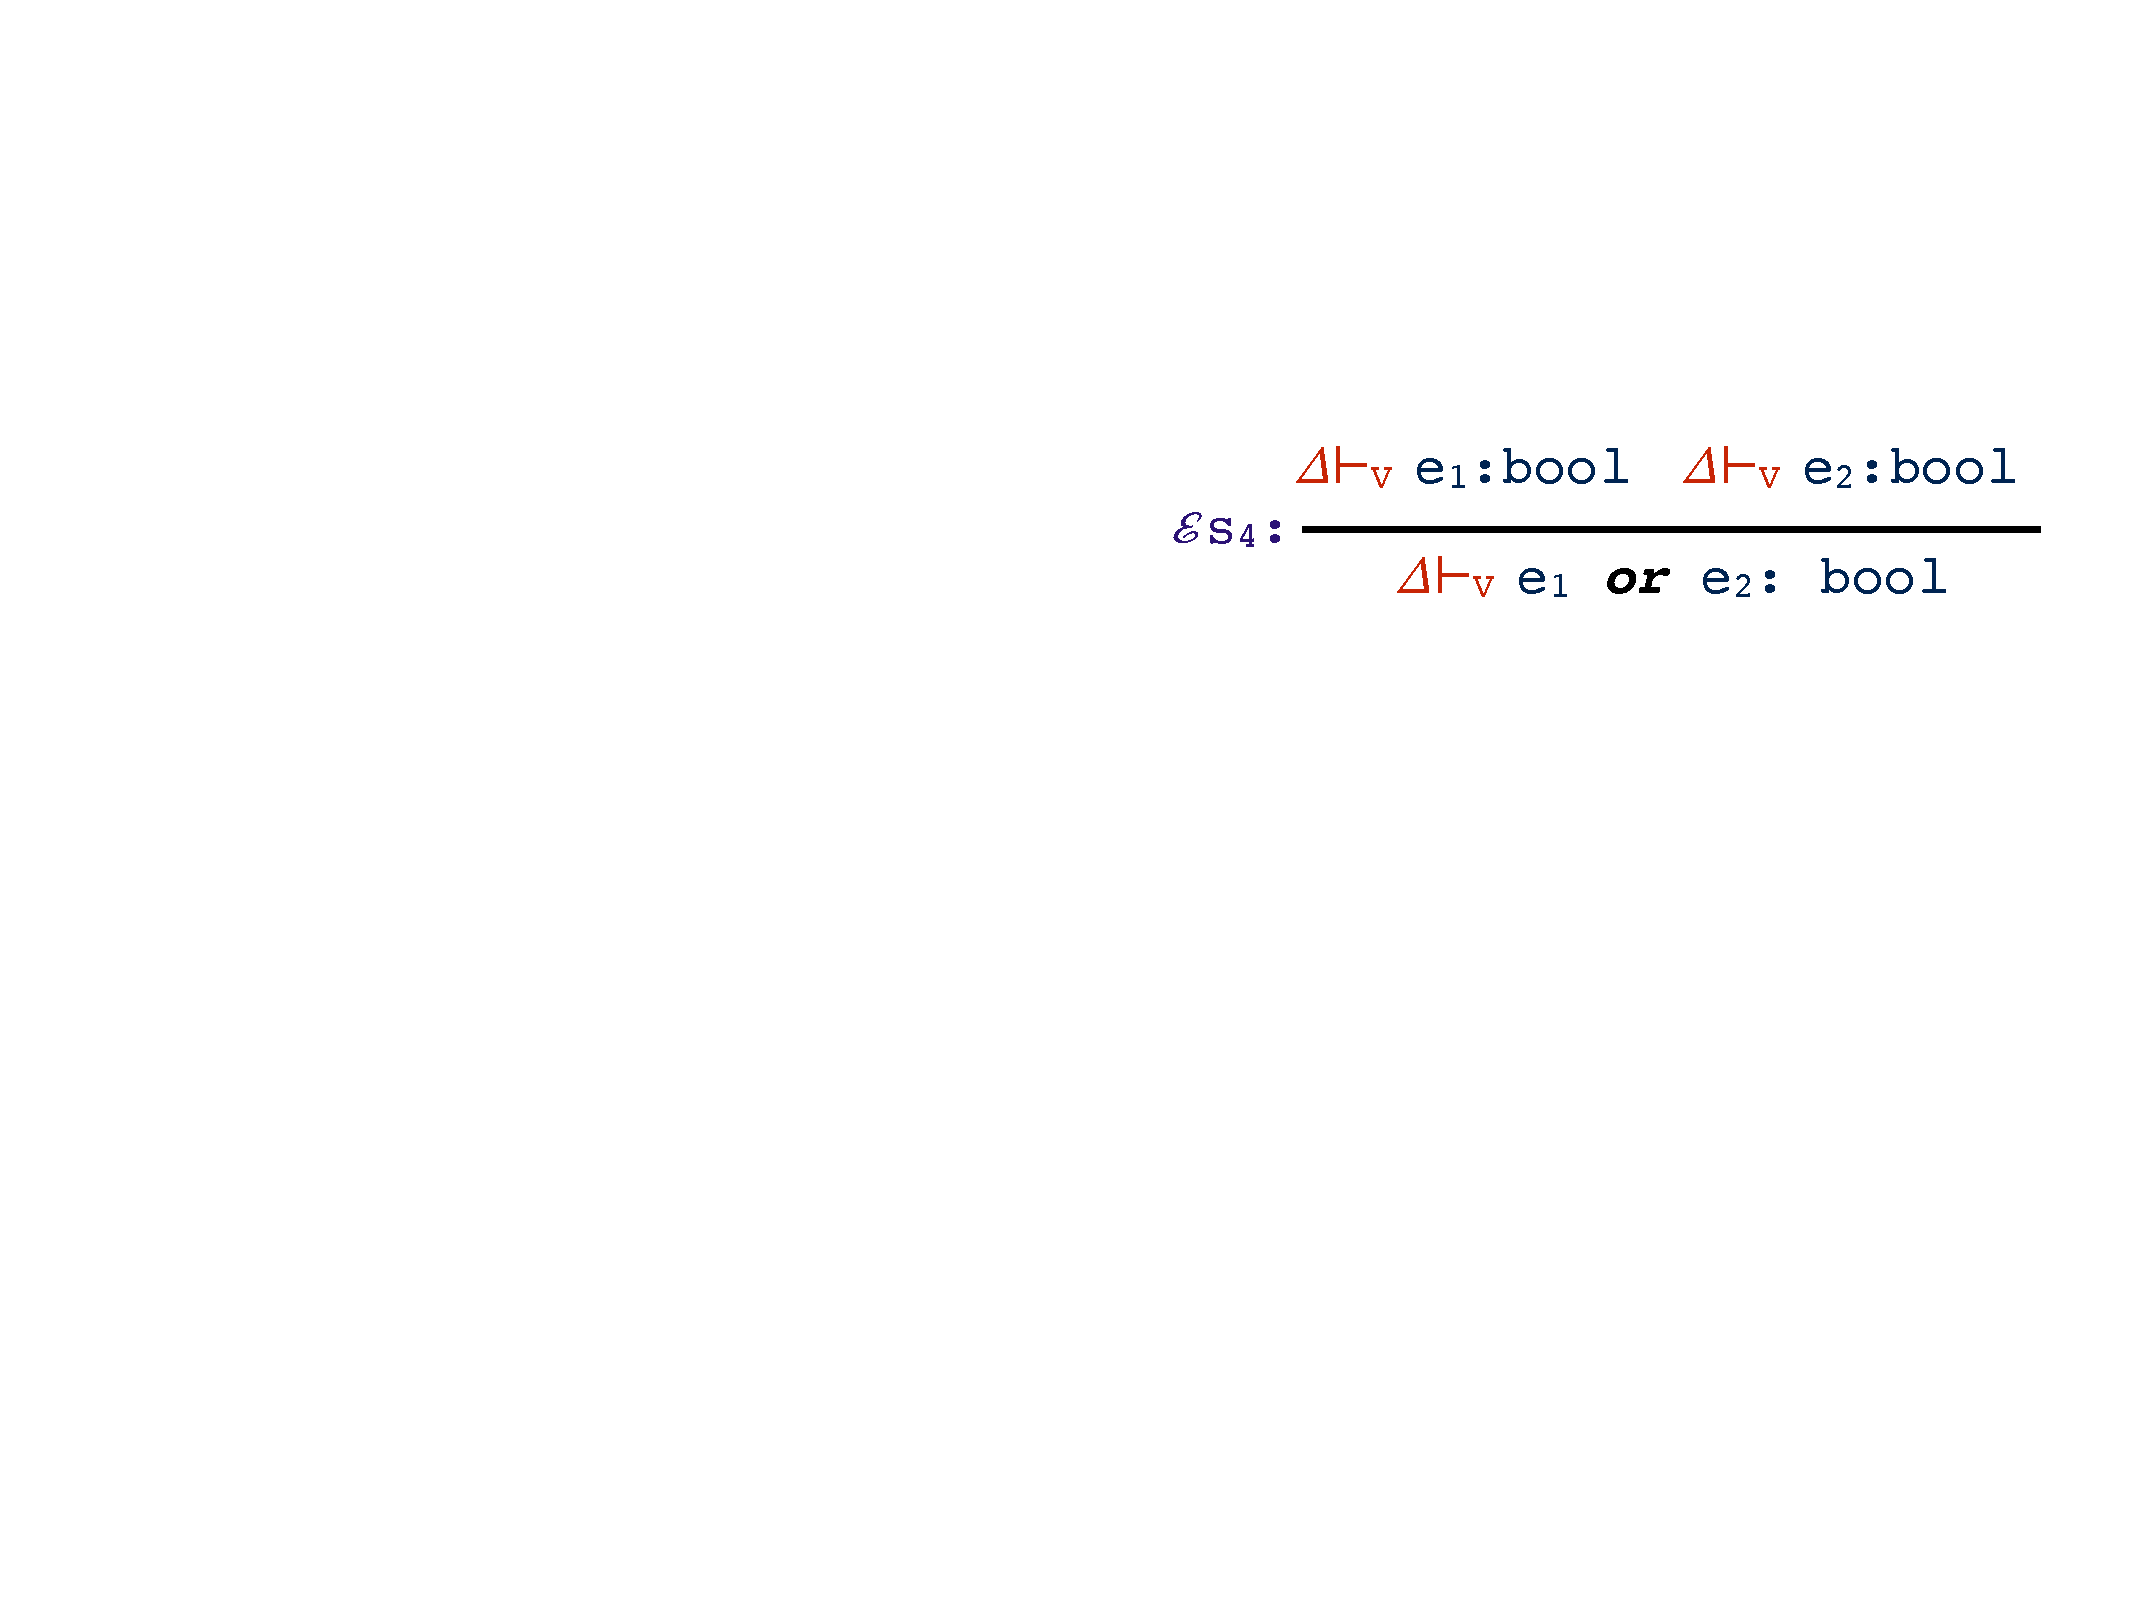
\includegraphics[width=.6\textwidth]{img/regola_semantica-4.pdf}
		\end{figure}
	
		\item La quinta regola:
		\begin{figure}[!htp]
			\centering
			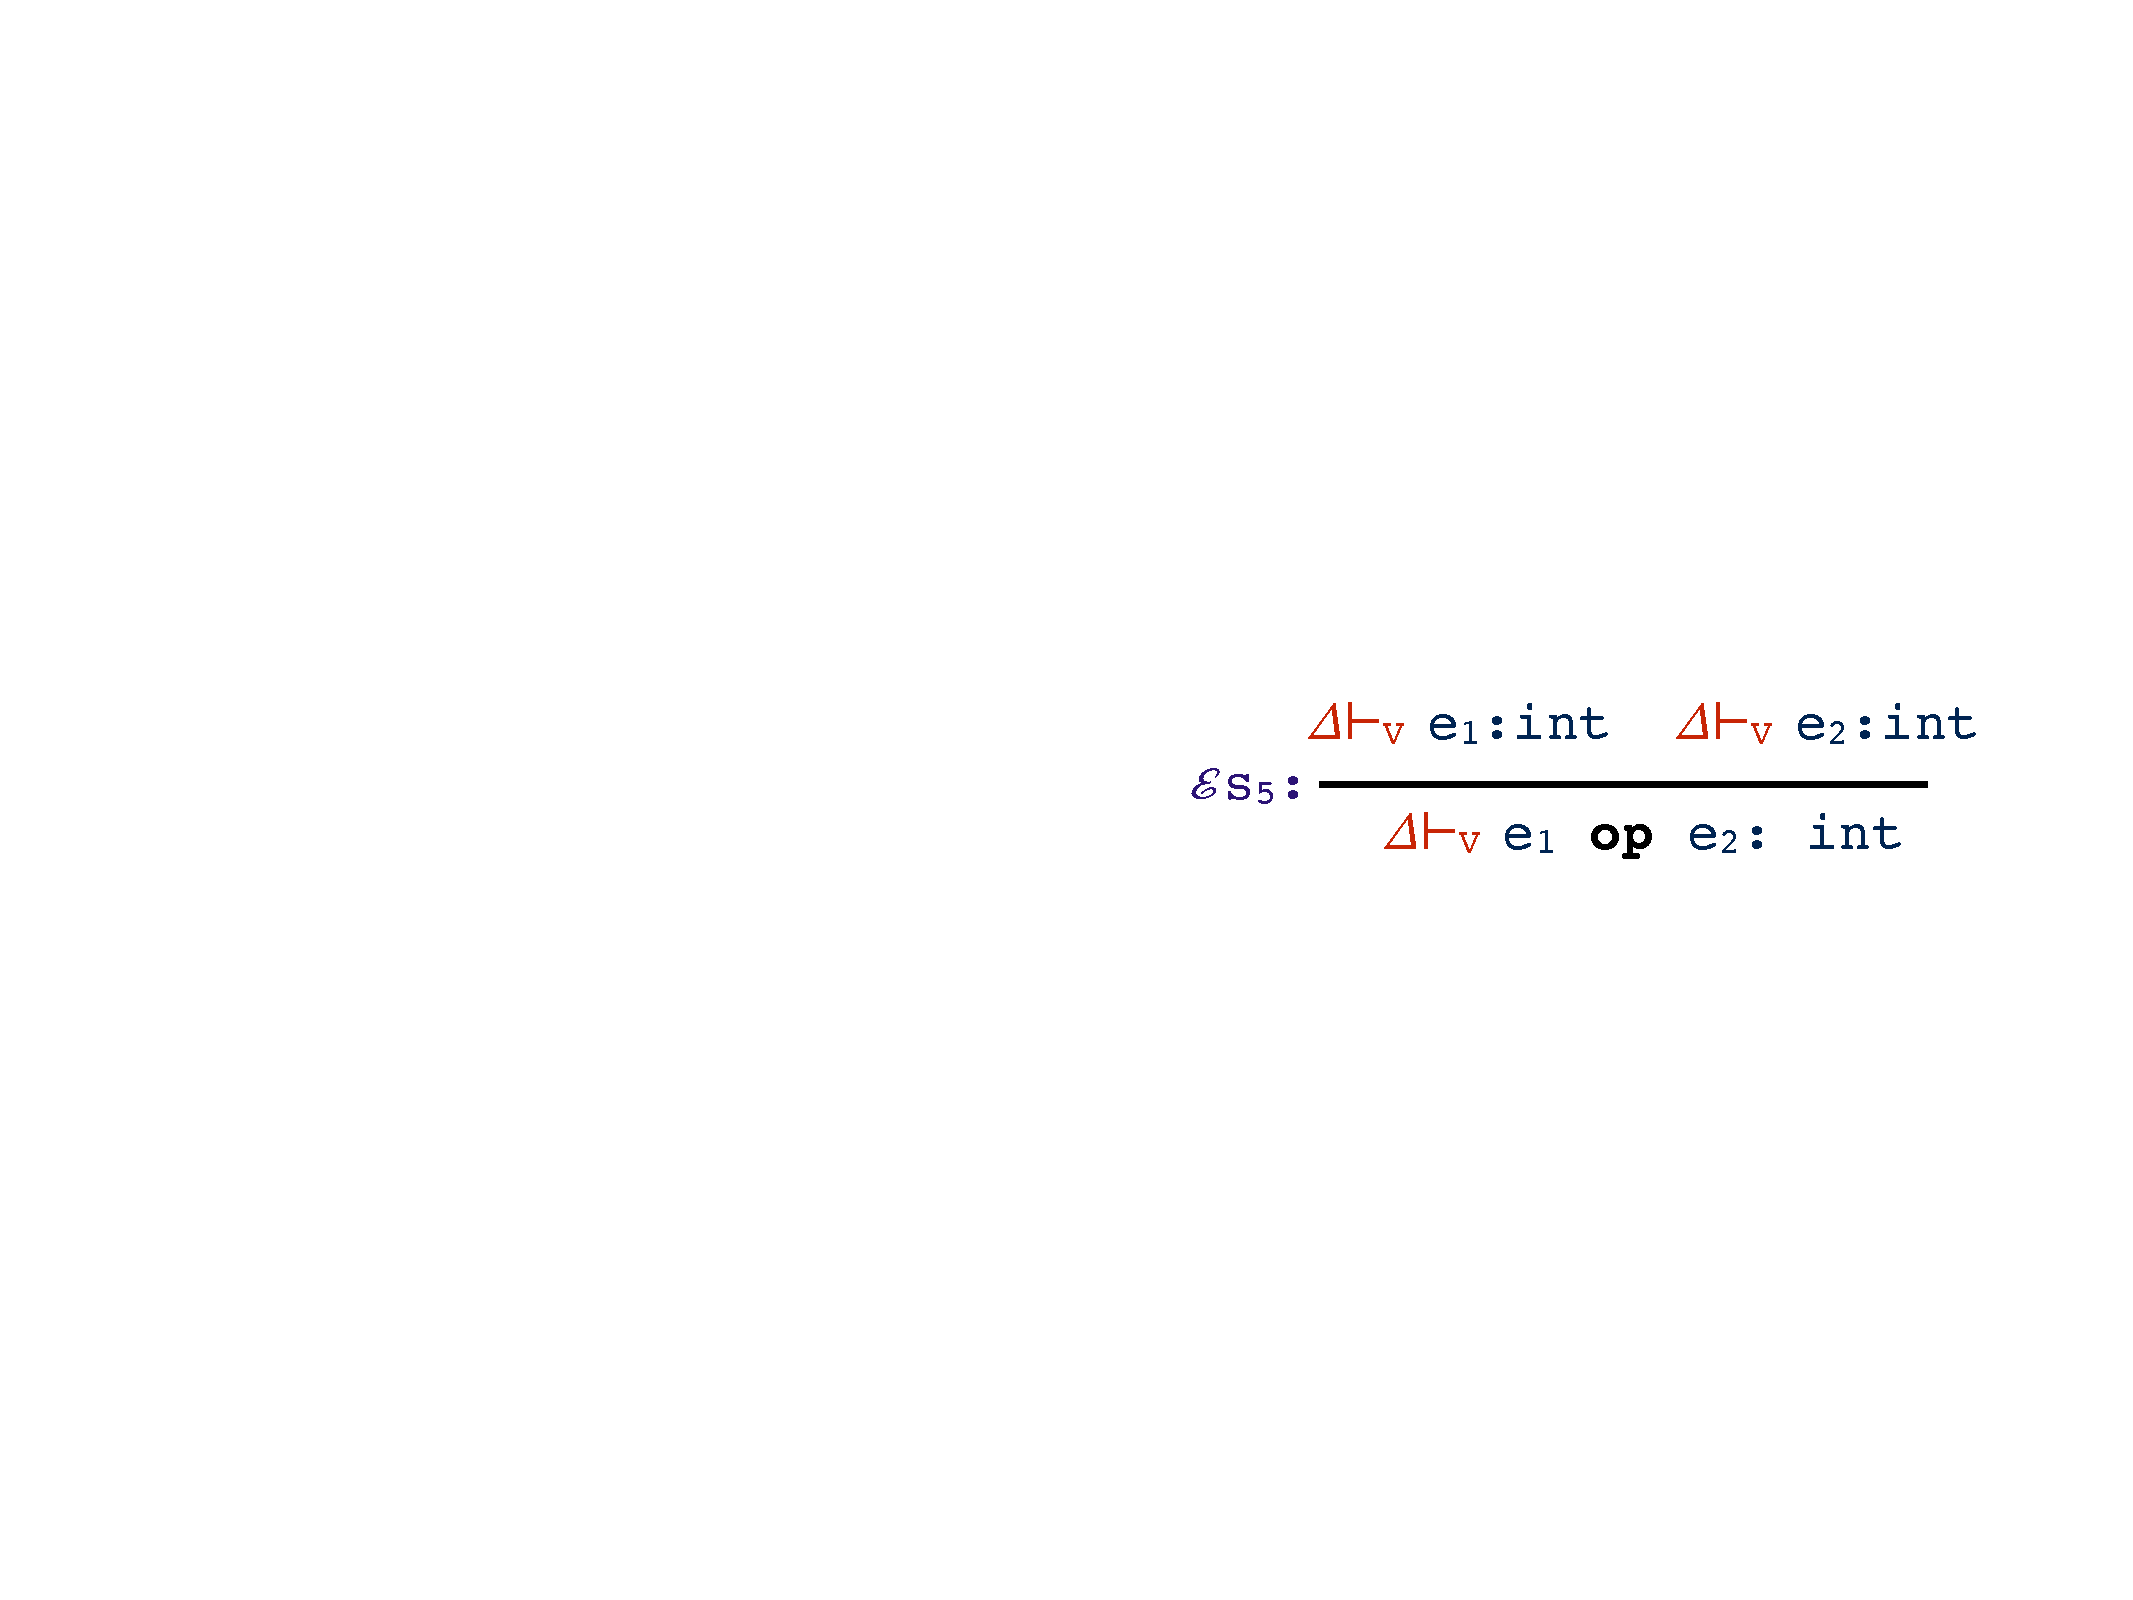
\includegraphics[width=.6\textwidth]{img/regola_semantica-5.pdf}
		\end{figure}
	
		\item La sesta regola:
		\begin{figure}[!htp]
			\centering
			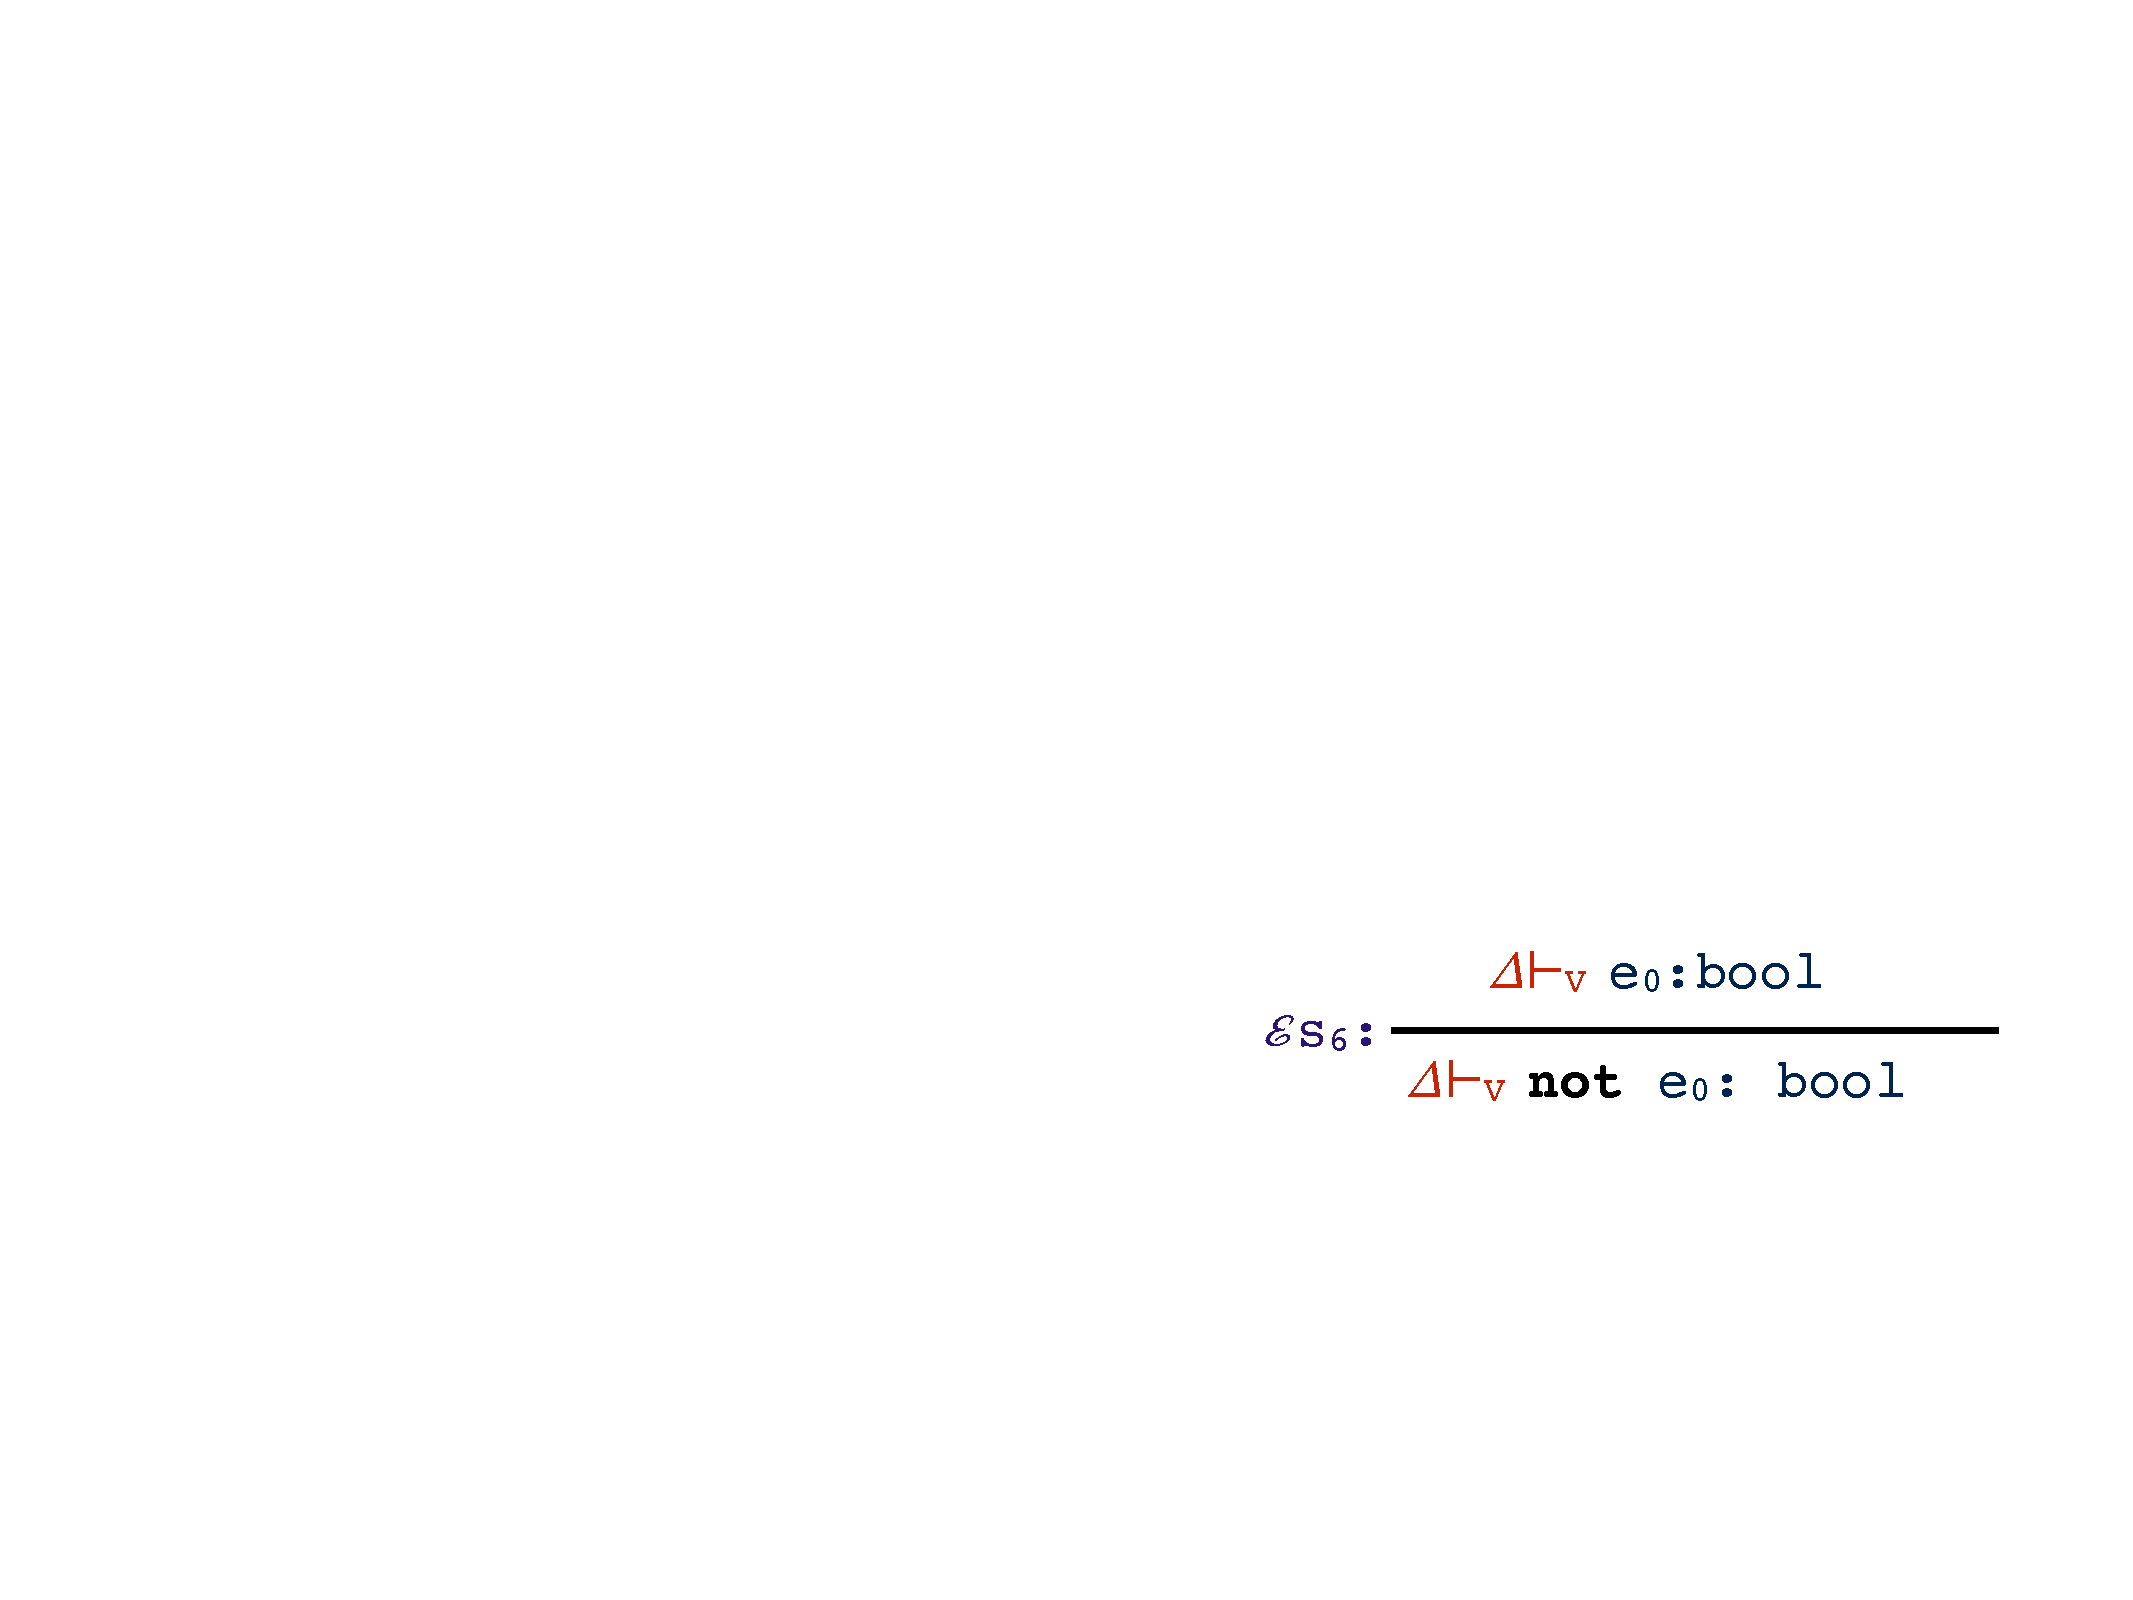
\includegraphics[width=.5\textwidth]{img/regola_semantica-6.pdf}
		\end{figure}\newpage
	
		\item La settima regola:
		\begin{figure}[!htp]
			\centering
			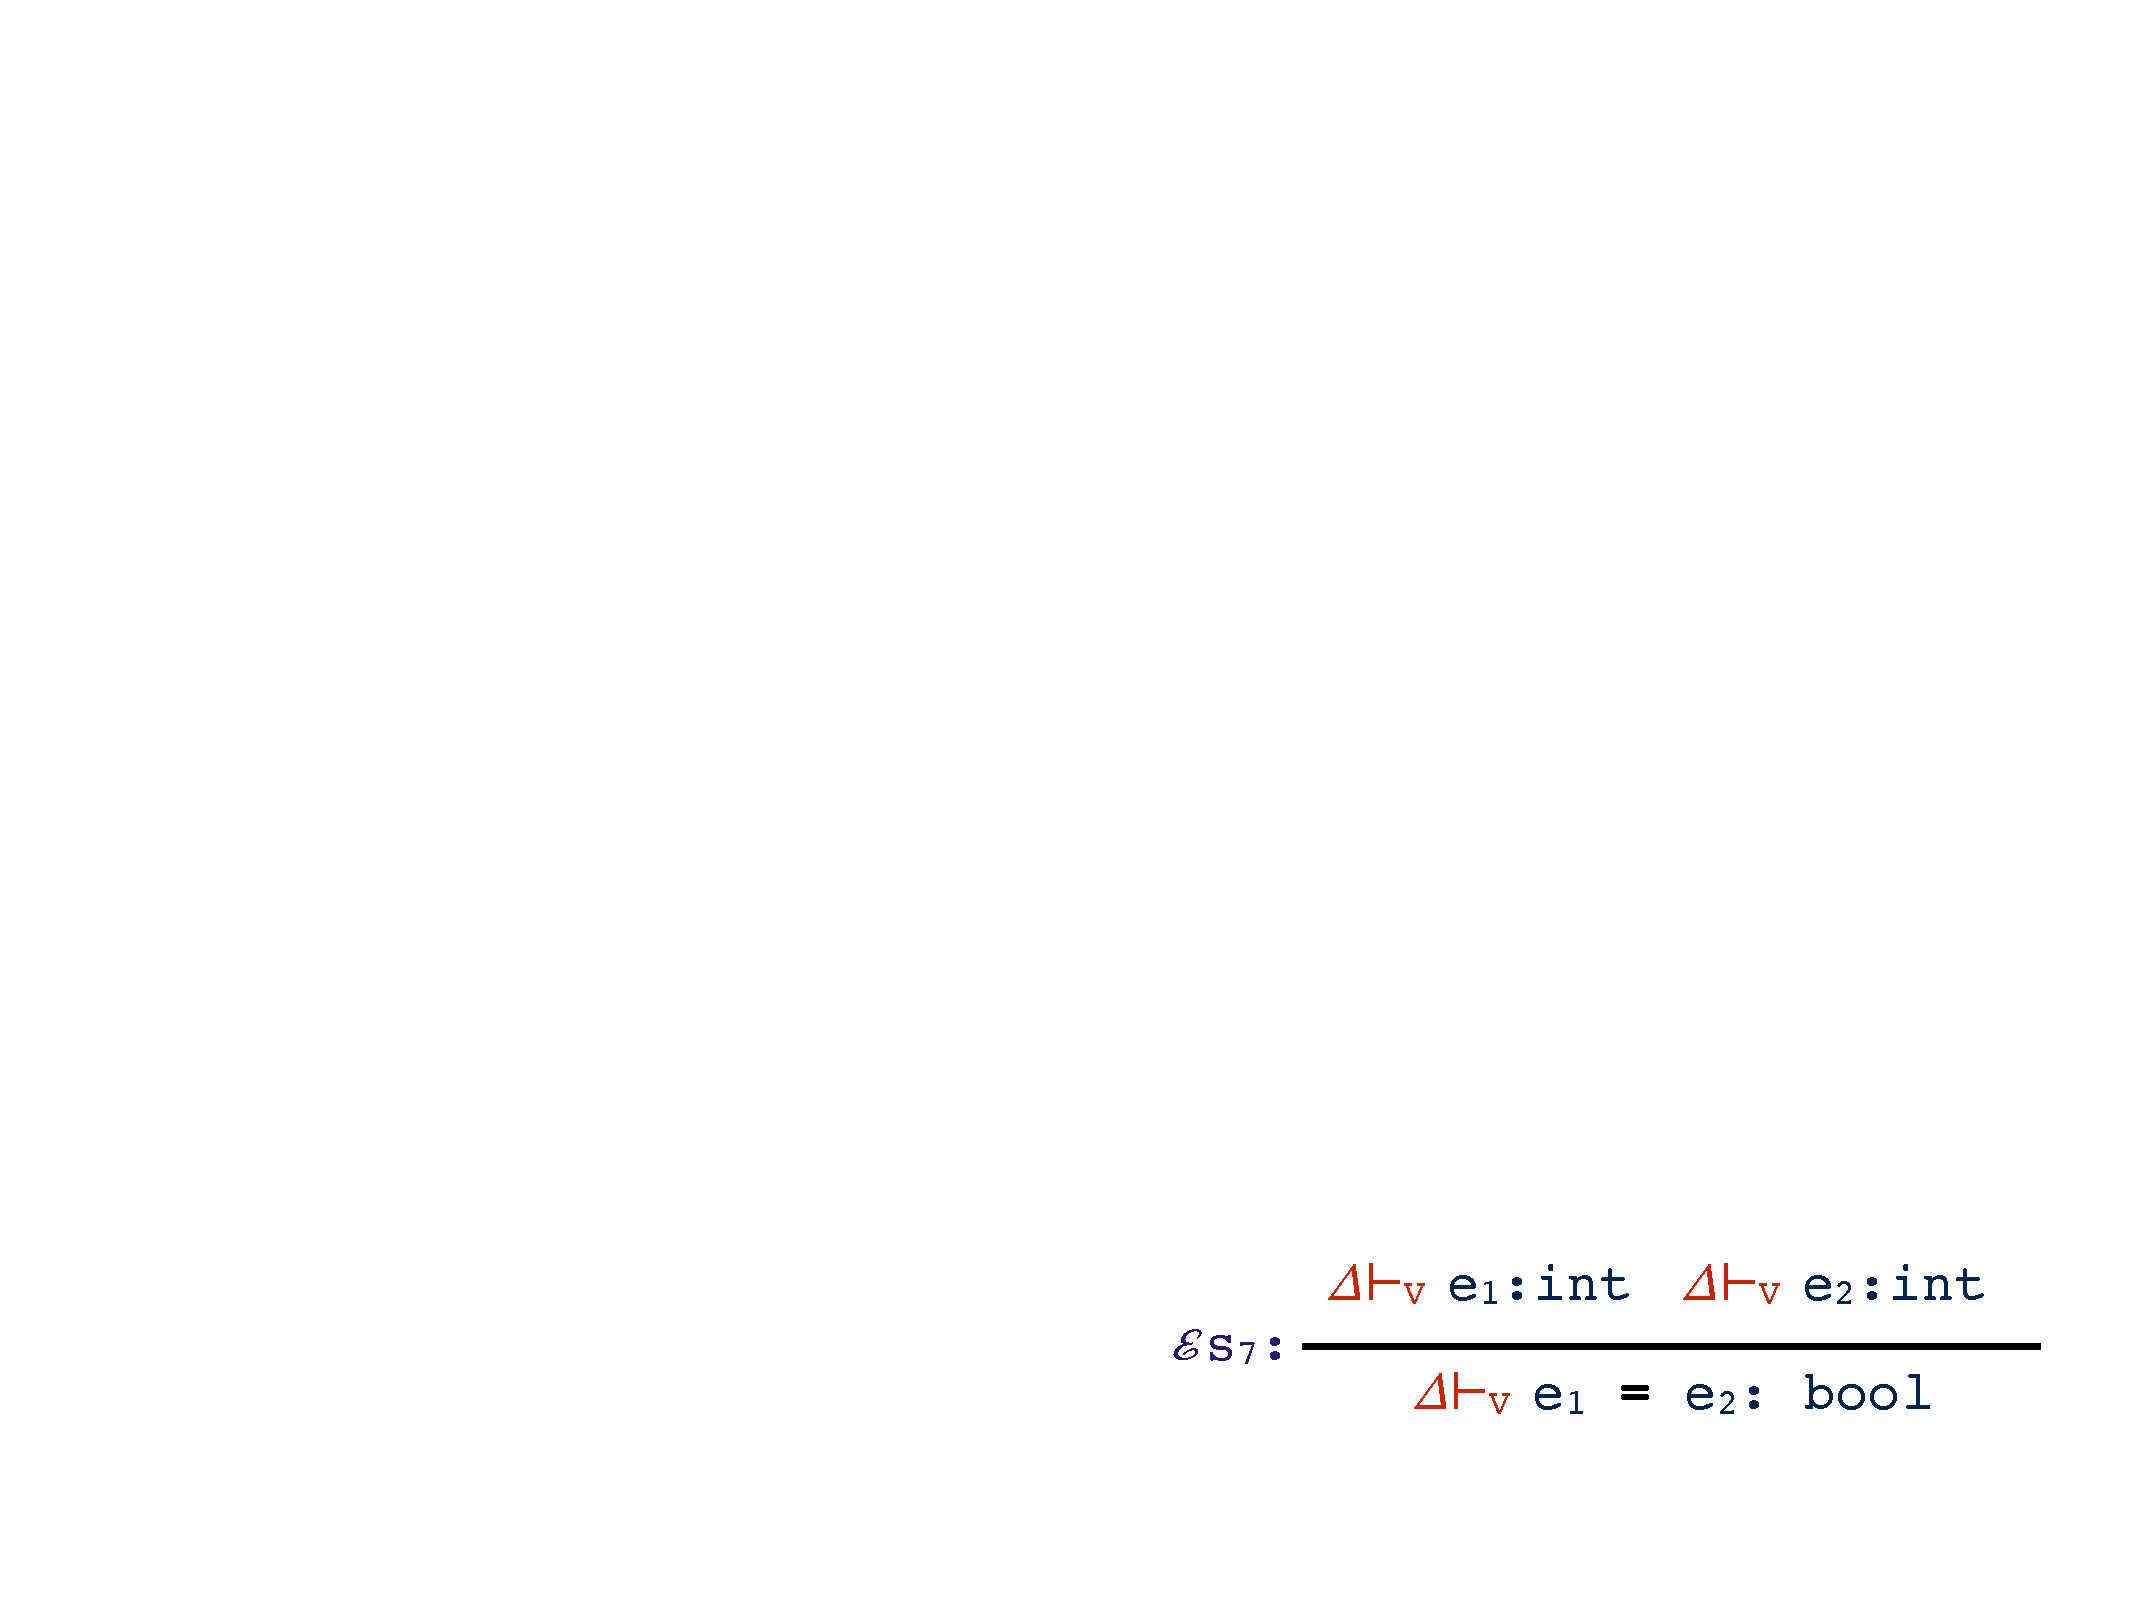
\includegraphics[width=.5\textwidth]{img/regola_semantica-7.pdf}
		\end{figure}
	\end{itemize}
	
	\longline
	
	\subsection{Compatibilità di ambienti e regole aggiornate}
	
	Date le due definizioni di ambiente statico e dinamico, è necessario introdurre una nuova definizione:
	\begin{boxdef}
		La \textcolor{Red3}{\textbf{compatibilità di ambienti}} è esprimibile nel seguente modo. Sia $\rho : V$ un ambiente dinamico e $\Delta : V$ un ambiente statico con $V \subseteq_{f} Id$. Gli ambienti $\rho$ e $\Delta$ sono compatibili (formalmente $\rho:\Delta$) se e soltanto se:
		\begin{equation*}
			\forall id \in V : \left( \Delta\left(id\right) = \tau \land \rho\left(id\right) \in \tau \right)
		\end{equation*}
		In una sola riga:
		\begin{equation*}
			\rho : \Delta \iff \forall id \in V : \left( \Delta\left(id\right) = \tau \land \rho\left(id\right) \in \tau \right)
		\end{equation*}
	\end{boxdef}
	
	\noindent
	Quindi, un ambiente statico e un ambiente dinamico sono \textbf{compatibili se \dquotes{parlano} in modo coerente degli stessi identificatori}. In particolare, questo significa che se l'ambiente statico stabilisce che una certa espressione ha tipo $\tau$, allora la semantica dinamica deve arrivare ad associare all'identificatore un valore contenuto nel tipo $\tau$, ovvero nell'insieme dei valori con lo stesso tipo $\tau$.\newline
	
	\noindent
	Adesso, nelle regole \textbf{non} si osserva più l'\textbf{ambiente dinamico} specificando l'insieme degli identificatori, ma specificando l'\textbf{ambiente statico compatibile}:
	\begin{equation*}
		\rho \dashv_{\Delta}
	\end{equation*}
	A seguito dell'aggiornamento con l'ambiente statico, si espongono le regole (paragrafo~\ref{nuove regole}) aggiornate tenendo in considerazione $op \in \left\{+,-,*,=\right\}$ e $bop \in \left\{or,=\right\}$:
	\begin{itemize}
		\item La prima regola:
		\begin{figure}[!htp]
			\centering
			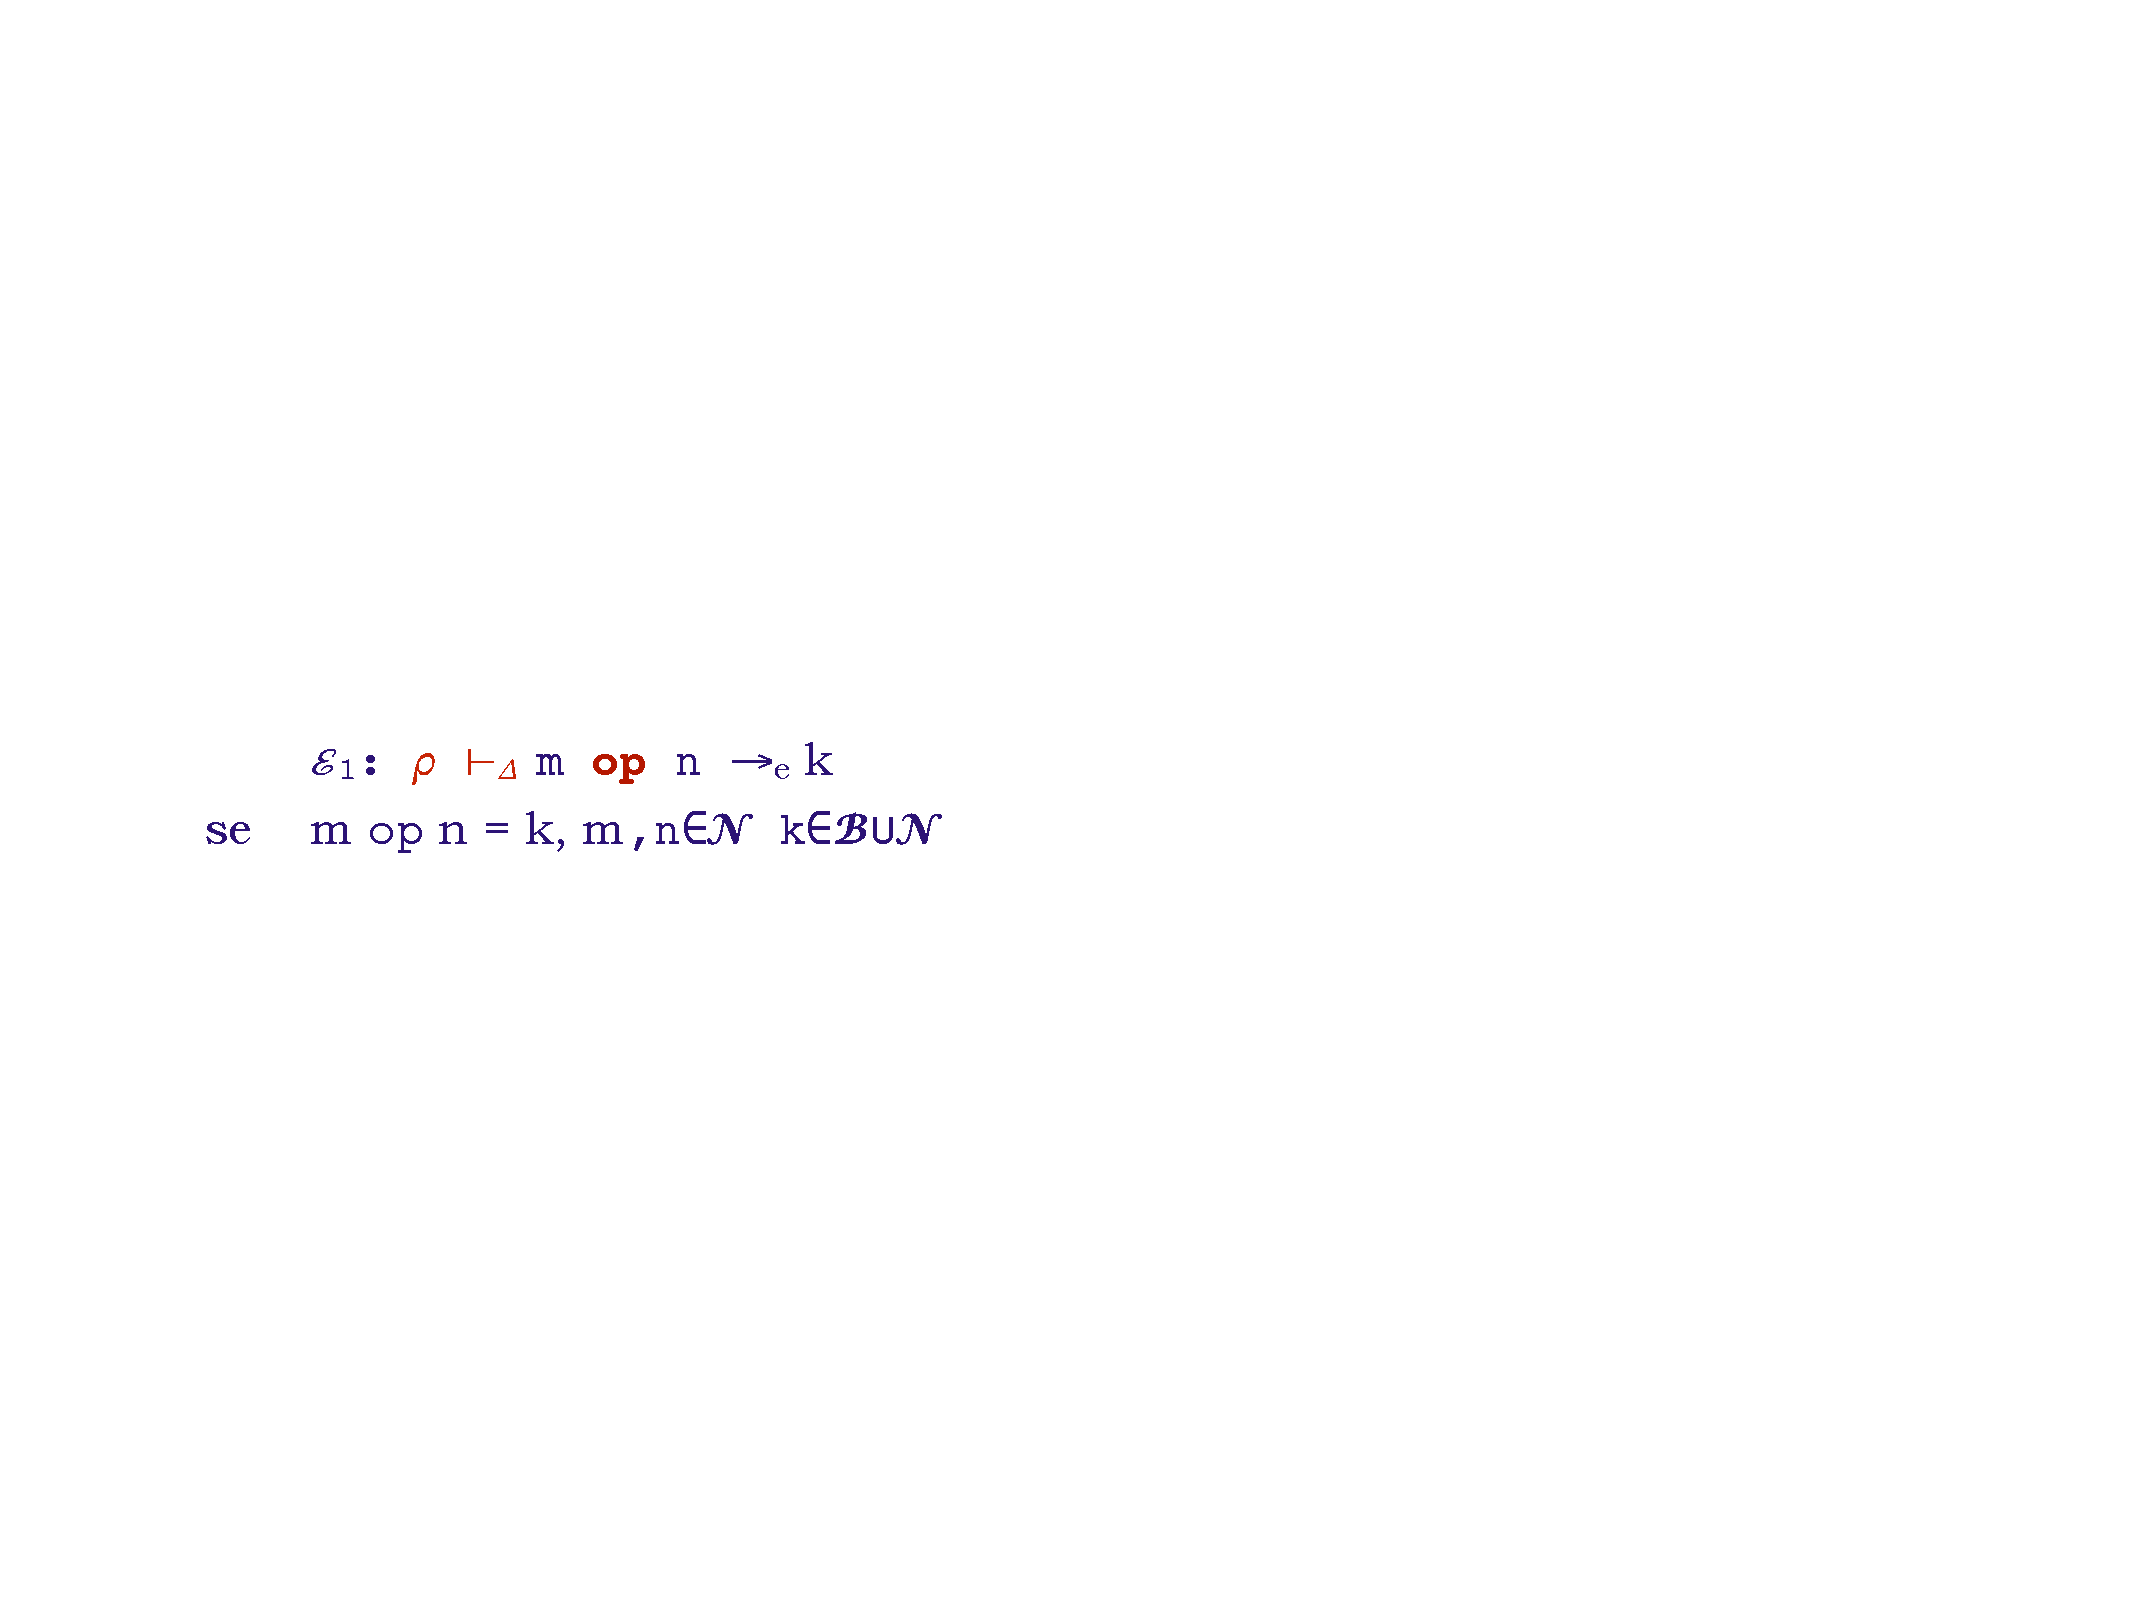
\includegraphics[width=.6\textwidth]{img/regola_espressione-mod-1.pdf}
		\end{figure}
		
		\item La seconda regola:
		\begin{figure}[!htp]
			\centering
			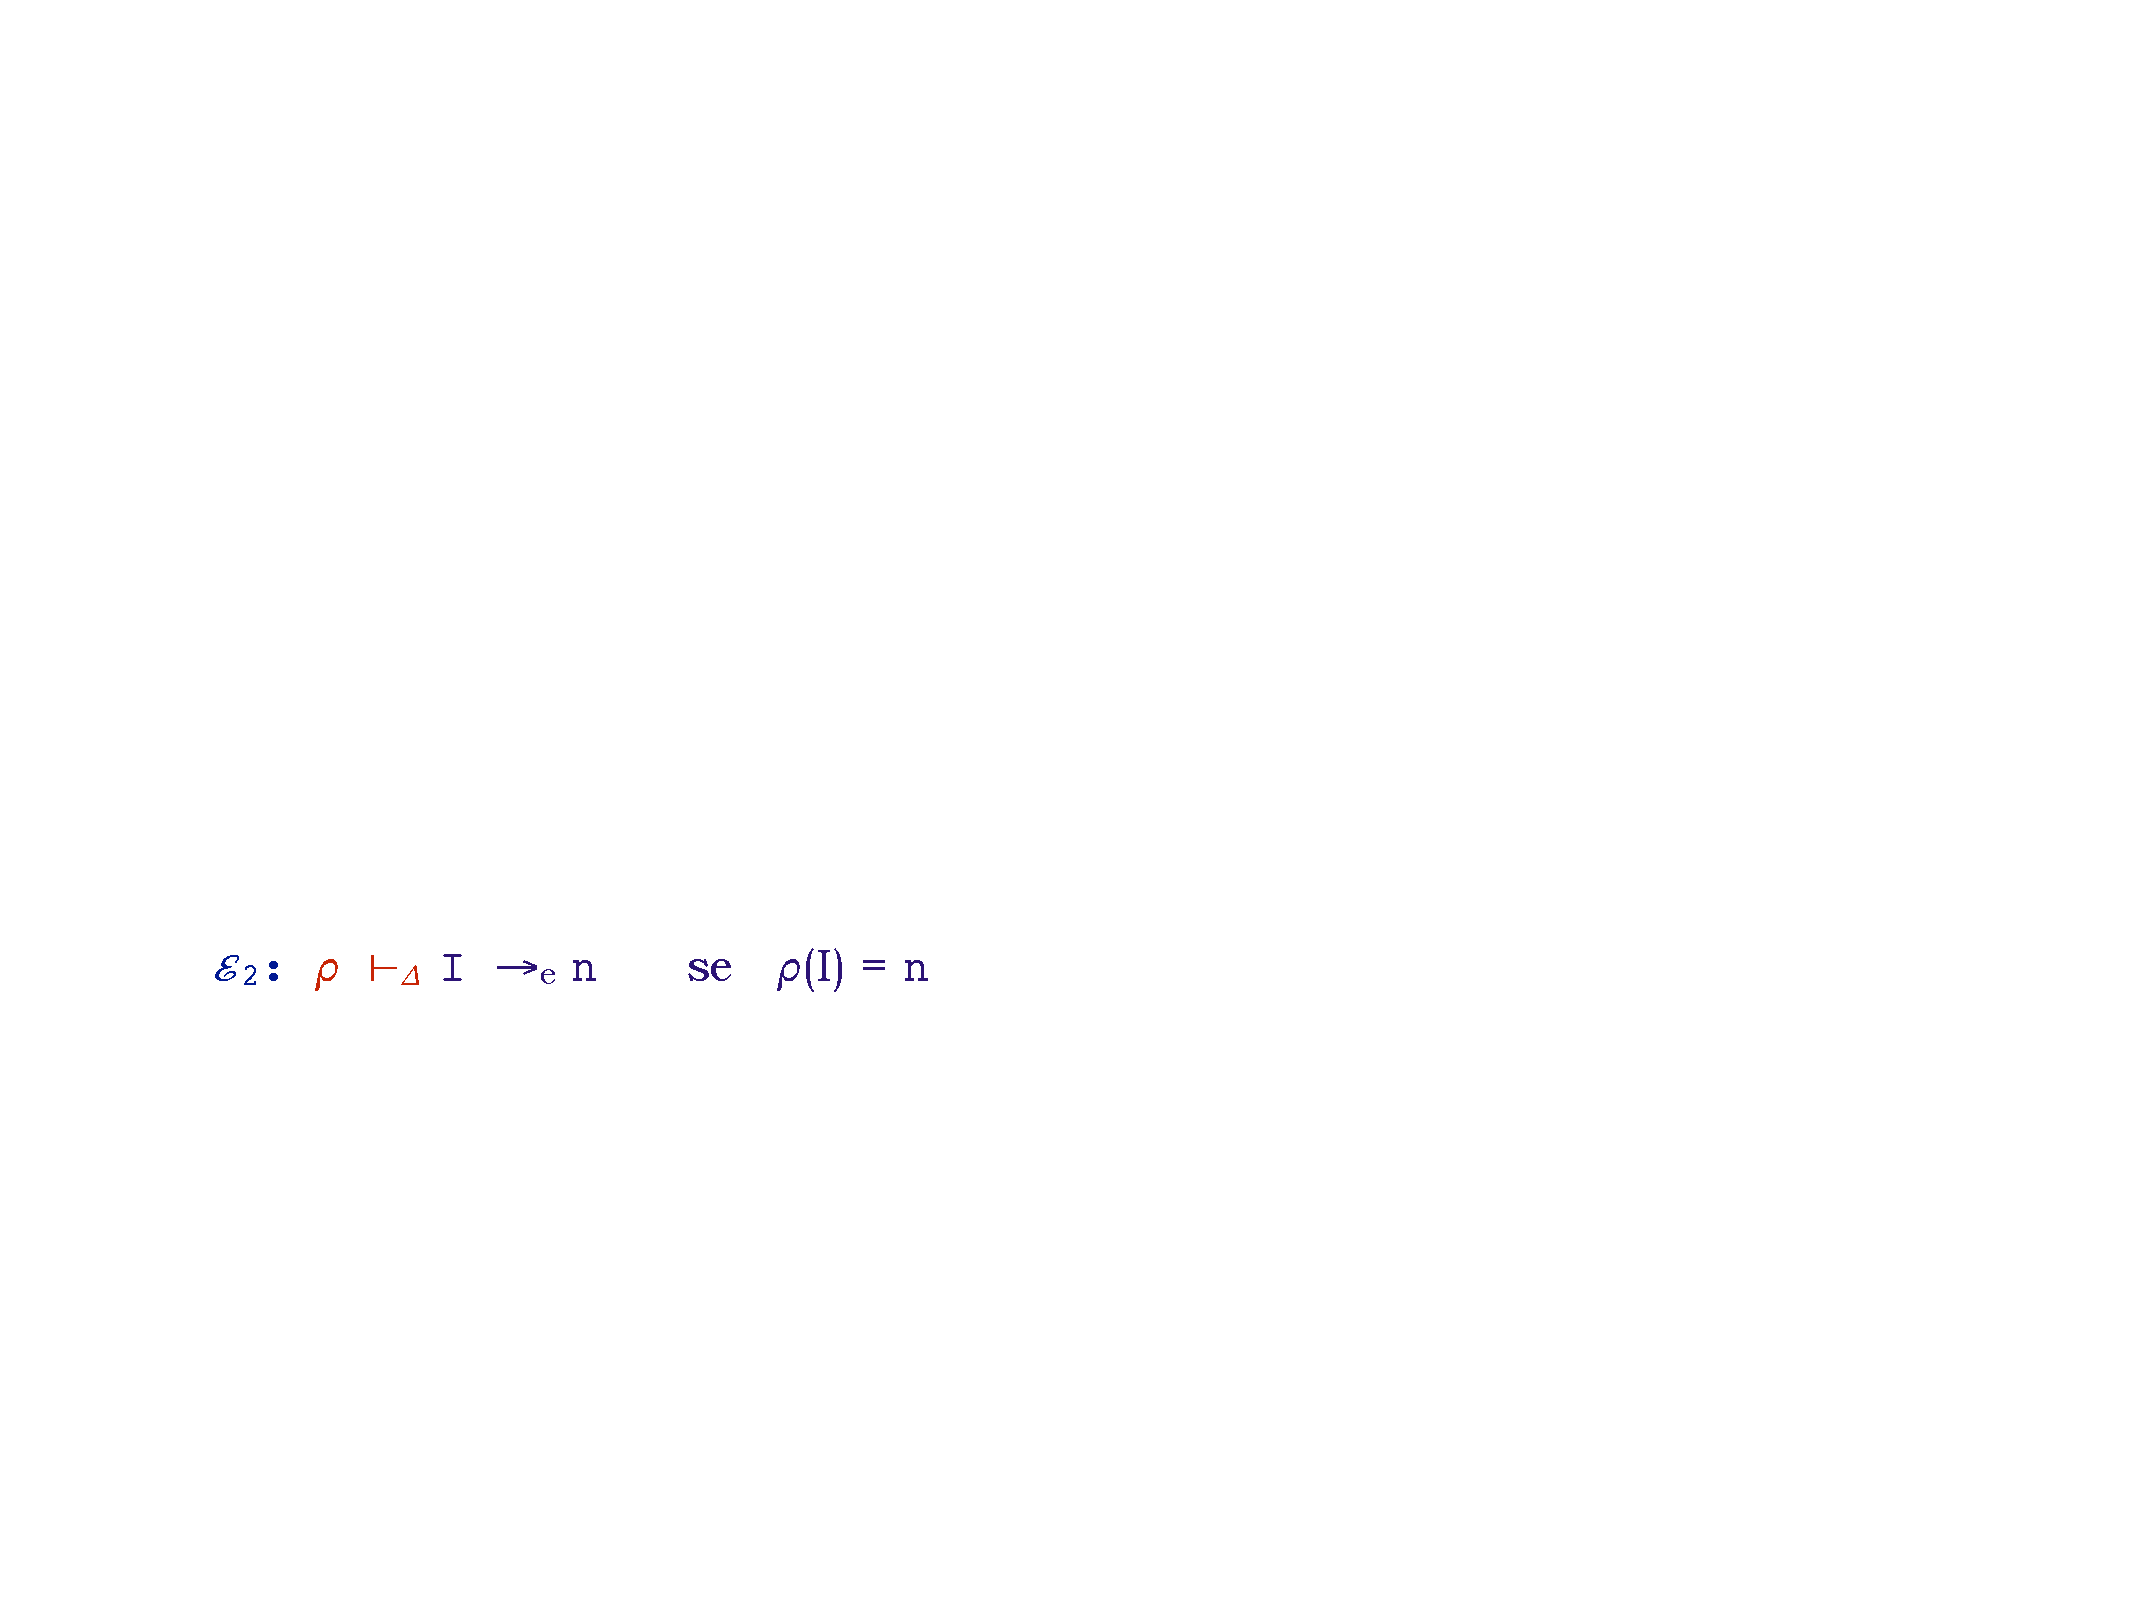
\includegraphics[width=.6\textwidth]{img/regola_espressione-mod-2.pdf}
		\end{figure}\newpage
		
		\item La terza regola:
		\begin{figure}[!htp]
			\centering
			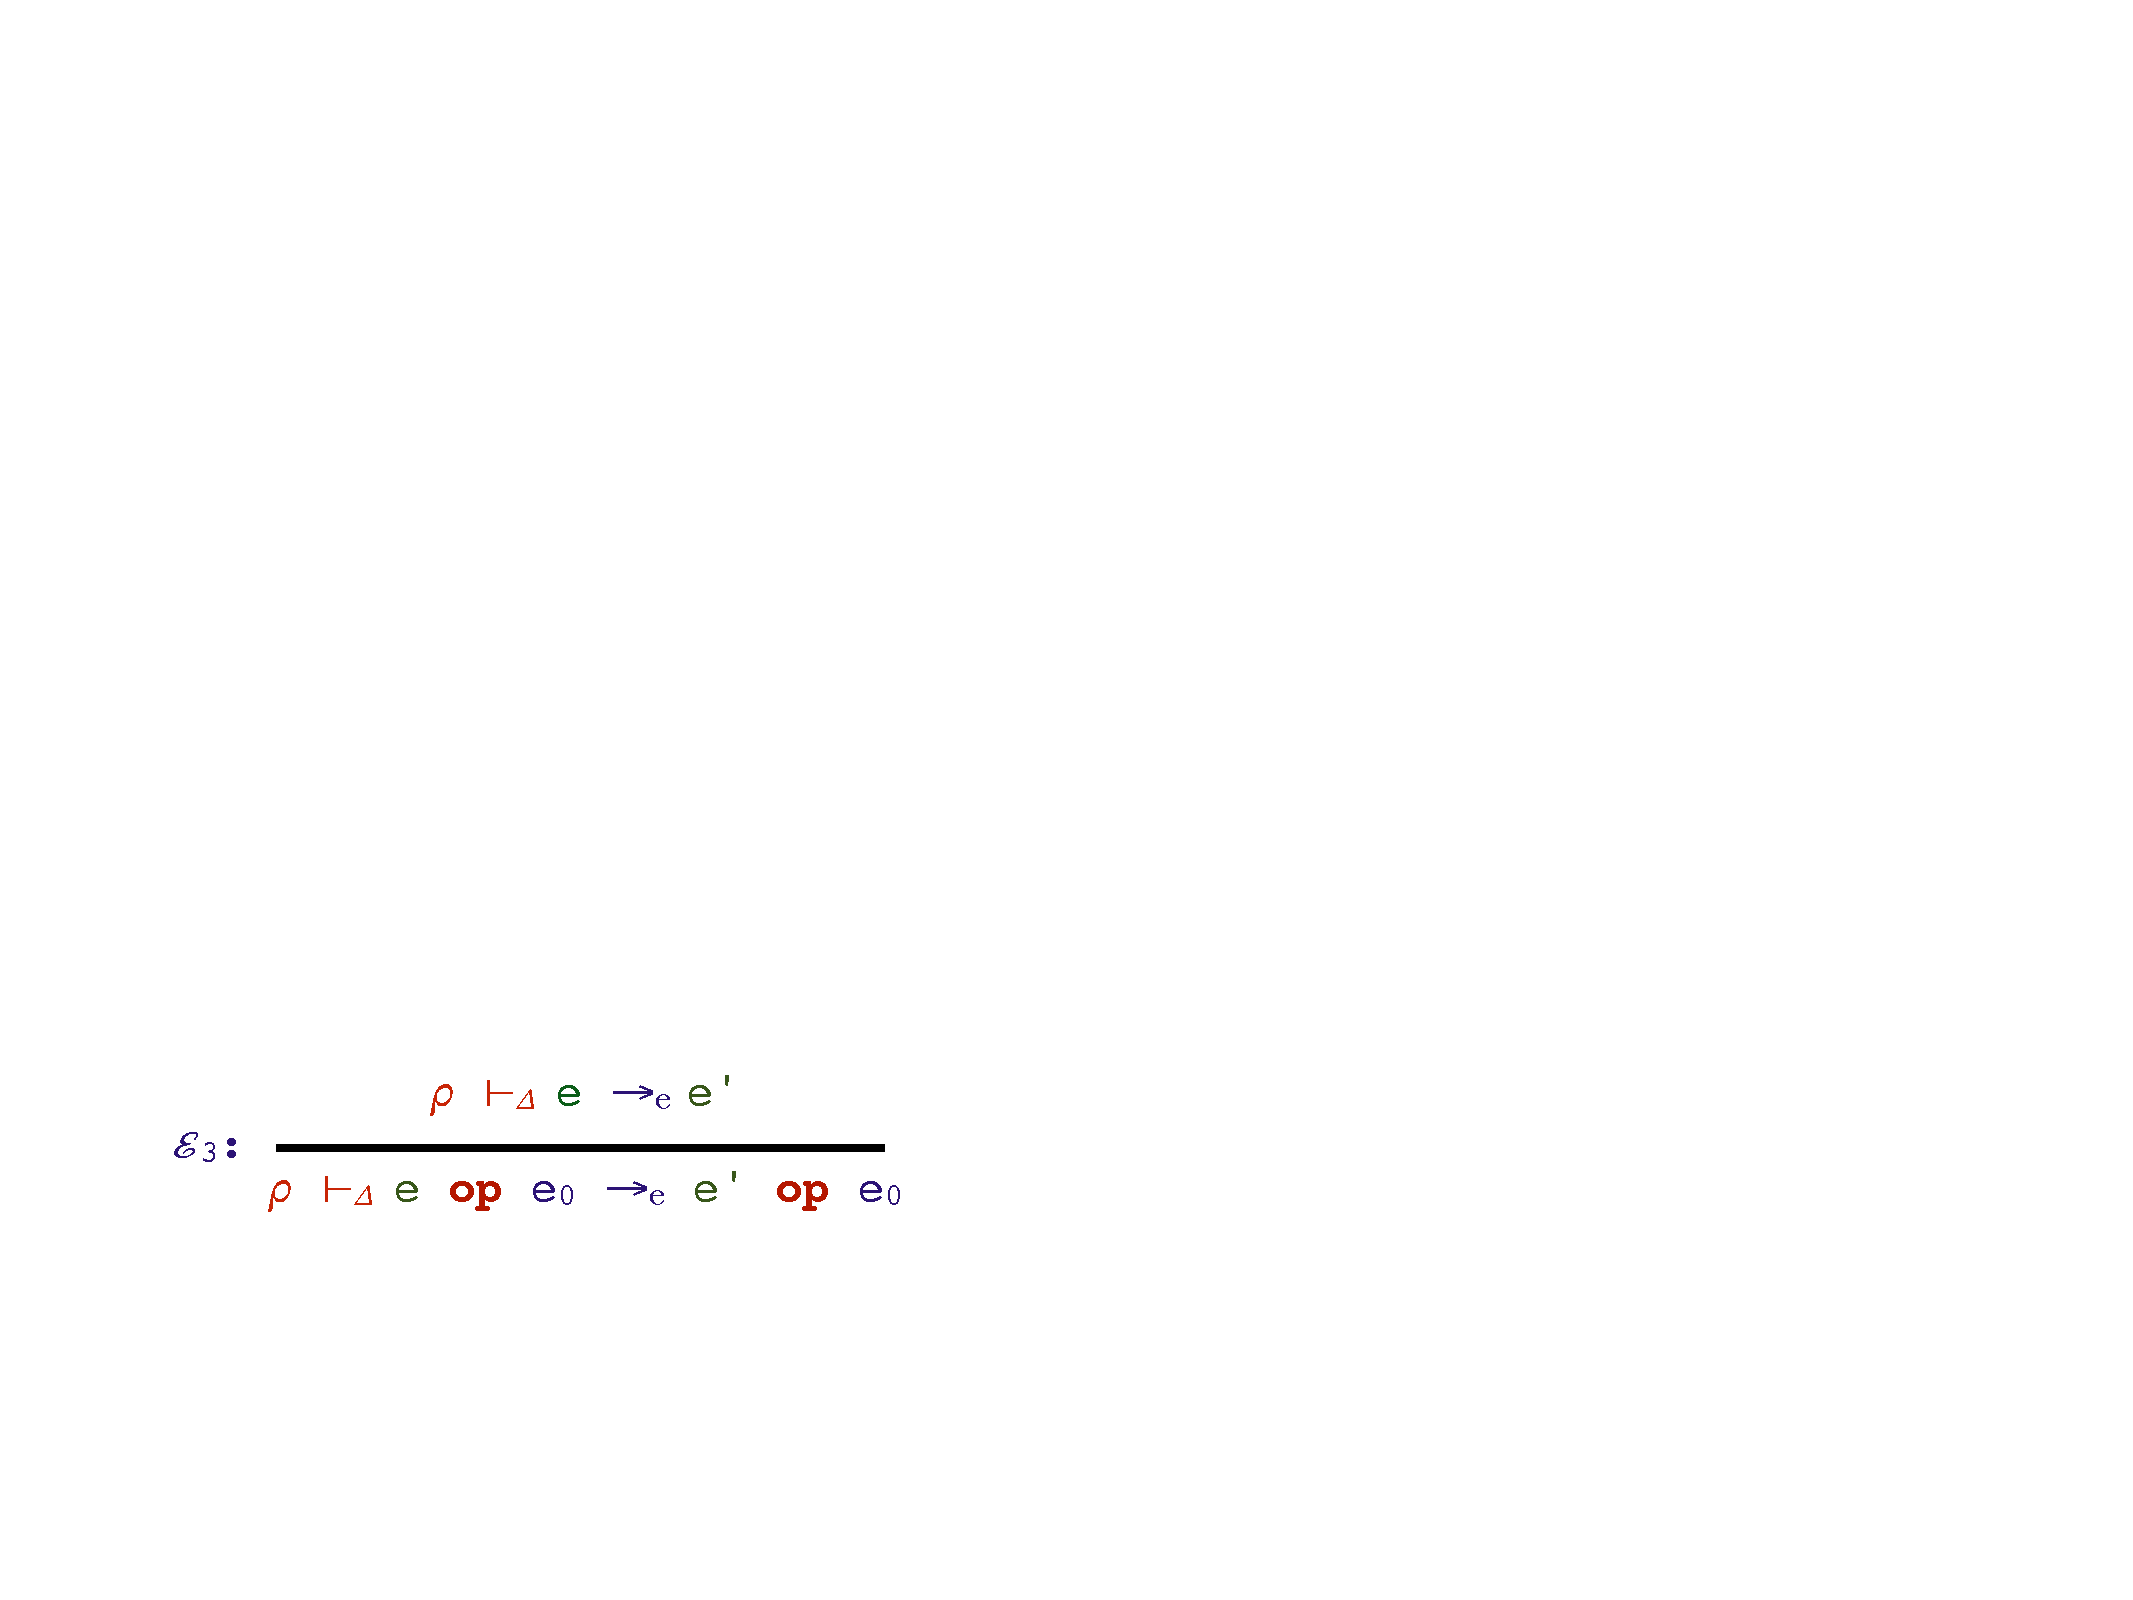
\includegraphics[width=.6\textwidth]{img/regola_espressione-mod-3.pdf}
		\end{figure}
		
		\item La quarta regola:
		\begin{figure}[!htp]
			\centering
			\includegraphics[width=.6\textwidth]{img/regola_espressione-mod-4.pdf}
		\end{figure}
		
		\item La terza regola aggiornata:
		\begin{figure}[!htp]
			\centering
			\includegraphics[width=.6\textwidth]{img/regola_espressione-mod-5.pdf}
		\end{figure}
		
		\item La sesta regola:
		\begin{figure}[!htp]
			\centering
			\includegraphics[width=.6\textwidth]{img/regola_espressione-mod-6.pdf}
		\end{figure}
		
		\item La settima regola:
		\begin{figure}[!htp]
			\centering
			\includegraphics[width=.6\textwidth]{img/regola_espressione-mod-7.pdf}
		\end{figure}
		
		\item L'ottava regola:
		\begin{figure}[!htp]
			\centering
			\includegraphics[width=.6\textwidth]{img/regola_espressione-mod-8.pdf}
		\end{figure}
	\end{itemize}\newpage
	
	\subsection{Dichiarazioni in $IMP$}
	
	Le dichiarazioni vengono \textbf{utilizzate per creare legami tra identificatori e oggetti denotati}. Le dichiarazioni quindi devono essere elaboratore per ottenere l'associazione che descrivono.\newline
	
	\noindent
	Si introduce la \textbf{sintassi delle dichiarazioni}, ovvero la loro \underline{\textbf{grammatica}}:
	\begin{equation*}
		\mathcal{D}: <Dec> \: D \rightarrow \mathrm{nil} \hspace{1em} | \hspace{1em} \mathrm{const} \: I:\tau = e \hspace{1em} | \hspace{1em} D \: \mathrm{in} \: D \hspace{1em} | \hspace{1em} D \: ; D \hspace{1em} | \hspace{1em} \rho
	\end{equation*}
	\begin{itemize}
		\item $D$ è il \textbf{simbolo non terminale della grammatica} che corrisponde (genera) tutti i termini della categoria sintattica, ovvero tutte le dichiarazioni nel linguaggio;
		
		\item $\mathrm{nil}$ è la \textbf{dichiarazione vuota}, ovvero quella che crea l'ambiente vuoto;
		
		\item $\mathrm{const} \: I:\tau = e$ è una \textbf{dichiarazione di una costante} che serve a definire un identificatore $I$ costante (quindi non cambia durante l'esecuzione) di tipo $\tau$, inizializzato con il valore rappresentato dall'espressione $e$.
		
		\item $\rho$ rappresenta la \textbf{dichiarazione completamente elaborata}, il suo \textbf{valore finale}, così come i simboli numerici erano i valori terminali delle espressioni.
		
		\item $D_{1} \: ; D_{2}$ definisce la \textbf{composizione sequenziale} dove $D_{1}$ definisce i legami che si uniscono a quelli di $D_{2}$ e che possono anche essere utilizzati da $D_{2}$.
		
		\item $D_{1} \: \mathrm{in} \: D_{2}$ definisce la \textbf{composizione privata}, ovvero i legami creati da $D_{1}$ sono visibili e utilizzati da $D_{2}$ ma non sono visibili all'esterno, dopo l'elaborazione di $D_{2}$. In altre parole, $D_{1}$ definisce i legami che risolvono le occorrenze libere presenti in $D_{2}$.
	\end{itemize}
	
	\begin{boxdef}
		Le \textcolor{Red3}{\textbf{dichiarazioni}} denotano richieste di modifica/creazione di ambienti.
	\end{boxdef}\newpage
	
	\subsubsection{Comporre dichiarazioni}
	
	Si definiscono graficamente le composizioni presentate nel paragrafo precedente, ovvero $D_{1} \: ; D_{2}$ e $D_{1} \: \mathrm{in} \: D_{2}$.\newline
	
	\noindent
	Nella \textbf{composizione sequenziale} tutto ciò che è definito dalla prima  è visibile alla seconda e dopo la dichiarazione, tranne ciò che la seconda sovrascrive:
	\begin{figure}[!htp]
		\centering
		\includegraphics[width=\textwidth]{img/composizione_sequenziale.pdf}
	\end{figure}

	\noindent
	Un \textcolor{Green4}{\textbf{esempio}} di \textbf{composizione sequenziale}:
	\begin{figure}[!htp]
		\centering
		\includegraphics[width=\textwidth]{img/esempio_composizione_sequenziale.pdf}
	\end{figure}
	
	\noindent
	Al contrario, nella \textbf{composizione privata} la prima dichiarazione è appunto privata, esclusiva, per la seconda:
	\begin{figure}[!htp]
		\centering
		\includegraphics[width=\textwidth]{img/composizione_privata.pdf}
	\end{figure}

	\noindent
	Un \textcolor{Green4}{\textbf{esempio}} di \textbf{composizione privata}:
	\begin{figure}[!htp]
		\centering
		\includegraphics[width=\textwidth]{img/esempio_composizione_privata.pdf}
	\end{figure}\newpage
	
	\subsubsection{Identificatori definiti nelle dichiarazioni}
	
	Si introducono gli \textcolor{Red3}{\textbf{identificatori definiti}}, ovvero identificatori in posizione di definizione. Si ricorda che l'obbiettivo primario delle dichiarazioni è quello di definire identificatori.\newline
	
	\noindent
	Quindi si definisce la funzione $DI$ (\emph{definite identificators}) che \textbf{associa ad ogni dichiarazione l'insieme degli identificatori} che definisce:
	\begin{equation*}
		DI: Dic \longrightarrow \wp\left(ID\right)
	\end{equation*}
	La definizione è induttiva sulla struttura delle dichiarazioni:
	\begin{itemize}
		\item La \textbf{\underline{dichiarazione nulla}} non definisce identificatori ed è un insieme vuoto:
		\begin{equation*}
			DI\left(\mathsf{nil}\right) = \emptyset
		\end{equation*}
		
		\item La \textbf{\underline{dichiarazione di costante}} definisce precisamente l'identificatore che sta dichiarando. Questo significa che dove questa dichiarazione è visibile, l'identificatore $x$ è legato a questa definizione:
		\begin{equation*}
			DI\left(\mathbf{const} \: \mathsf{x}: \tau = \mathrm{e}\right) = \left\{x\right\}
		\end{equation*}
		
		\item La \textbf{\underline{composizione sequenziale}} definisce tutto ciò che è definito nelle due dichiarazioni. Questo significa che all'esterno della composizione tutte le occorrenze di identificatori qui definiti sono legate:
		\begin{equation*}
			DI\left(d_{1} ; d_{2}\right) = DI\left(d_{1}\right) \cup DI\left(d_{2}\right)
		\end{equation*}
		
		\item La \textbf{\underline{composizione privata}} è particolare. Ciò che viene definito nella prima dichiarazione $d_{1}$ rimane privato e quindi non risulta legato all'esterno della composizione. Fuori dalla composizione è legato solo ciò che viene definito nella seconda dichiarazione $d_{2}$:
		\begin{equation*}
			DI\left(d_{1} \: \mathsf{in} \: d_{2}\right) = DI\left(d_{2}\right)
		\end{equation*}
		
		\item Il \textbf{\underline{valore terminale}}, ovvero gli ambienti, definiscono tutti gli identificatori per i quali hanno una associazione:
		\begin{equation*}
			DI\left(\rho\right) = V
		\end{equation*}
		Dove $V$ è il dominio di $\rho$.
	\end{itemize}\newpage
	
	\subsubsection{Identificatori liberi nelle dichiarazioni}
	
	Al contrario degli identificatori definiti, gli \textcolor{Red3}{\textbf{identificatori liberi}} si trovano fuori dallo scope di una qualche dichiarazione/definizione.\newline
	
	\noindent
	Gli \textbf{identificatori liberi}, calcolati dalla funzione $FI$ (\emph{free identificators}), si possono ottenere anche sulle dichiarazioni, per induzione sulla struttura della grammatica. In questo caso, $FI$ \textbf{applicata ad una dichiarazione restituisce l'insieme degli identificatori liberi nella dichiarazione}:
	\begin{equation*}
		FI: Dic \longrightarrow \wp\left(Id\right)
	\end{equation*}
	In particolare:
	\begin{itemize}
		\item La \textbf{\underline{dichiarazione nulla}} non ha identificatori e non ne ha liberi dunque:
		\begin{equation*}
			FI\left(\mathsf{nil}\right) = \emptyset
		\end{equation*}
		
		\item La \textbf{\underline{identificatori liberi}} della dichiarazione di costante sono tutti quelli usati nell'espressione che inizializza l'identificatore. Questi identificatori devono essere definiti nell'ambiente di elaborazione perché si possa valutare l'espressione:
		\begin{equation*}
			FI\left(\mathbf{const} \: \mathsf{x}: \tau = \mathrm{e}\right) = FI\left(\mathrm{e}\right)
		\end{equation*}
		
		\item Il \textbf{\underline{caso delle due composizioni}} sono sicuramente liberi tutti gli identificatori della prima dichiarazione $d_{1}$. Sono inoltre liberi tutti gli identificatori che sono liberi nella seconda dichiarazione $d_{2}$ ma che non vengono definiti in $d_{1}$:
		\begin{gather*}
			FI\left(d_{1} ; d_{2}\right) = FI\left(d_{1}\right) \cup \left(FI\left(d_{2}\right) \setminus DI\left(d_{1}\right)\right) \\
			FI\left(d_{1} \: \mathsf{in} \: d_{2}\right) = FI\left(d_{1}\right) \cup \left(FI\left(d_{2}\right) \setminus DI\left(d_{1}\right)\right)
		\end{gather*}
		
		\item Un \textbf{\underline{ambiente non ha identificatori liberi}}, in quanto gli unici identificatori che contiene sono quelli per cui definisce delle associazioni:
		\begin{equation*}
			FI\left(\rho\right) = \emptyset
		\end{equation*}
	\end{itemize}\newpage
	
	\subsubsection{Semantica statica delle dichiarazioni}
	
	Per le dichiarazioni, la \textbf{semantica statica deve associare un ambiente statico ad ogni dichiarazione scritta correttamente} (chiamata ben formata). Le regole, sempre per quanto riguarda le dichiarazioni, dovranno avere la seguente forma:
	\begin{figure}[!htp]
		\centering
		\includegraphics[width=.3\textwidth]{img/semantica_statica_dichiarazioni.pdf}
	\end{figure}

	\noindent
	Vuol dire che nel sistema di regole è possibile associare l'ambiente statico $\Delta$ alla dichiarazione $d$, se questa è ben formata.\newline
	
	\noindent
	Si introducono qua di seguito le \textbf{regole}:
	\begin{itemize}
		\item La \textbf{dichiarazione vuota} genera un ambiente vuoto:
		\begin{figure}[!htp]
			\centering
			\includegraphics[width=.3\textwidth]{img/semantica_statica_dichiarazioni-1.pdf}
		\end{figure}
		
		\item Con un \textbf{ambiente dinamico}, l'ambiente statico associato è quello compatibile, ovvero quello che associa agli identificatori esattamente i tipi dei valori che l'ambiente dinamico associa:
		\begin{figure}[!htp]
			\centering
			\includegraphics[width=.4\textwidth]{img/semantica_statica_dichiarazioni-2.pdf}
		\end{figure}
		
		\item Nella \textbf{dichiarazione di costante}, il tipo da associare è stabilito esplicitamente dalla dichiarazione. Quest'ultima viene detta ben formata se rispetta quanto scritto a pagina~\ref{ben formata} ed è esattamente del tipo $\tau$ presente nella dichiarazione. In tal caso l'ambiente statico corrispondente è esattamente l'associazione di $\tau$ all'identificatore definito $x$:
		\begin{figure}[!htp]
			\centering
			\includegraphics[width=.5\textwidth]{img/semantica_statica_dichiarazioni-3.pdf}
		\end{figure}
	\end{itemize}\newpage

	\noindent
	Si considerino due ambiente $\beta$, $\beta' \in Env$ dove $\beta : V, \beta' : V'$ (cioè compatibili) con $V,V' \subseteq Id$, dove:
	\begin{itemize}
		\item $\beta$ è definito sugli identificatori in $V$	
		\item $\beta'$ è definito sull'insieme di identificatori $V'$
	\end{itemize}
	L'aggiornamento dell'ambiente $\beta$ mediante l'ambiente $\beta'$ dà come risultato l'ambiente $\beta''\in Env$, denotato con $\beta\left[\beta'\right]$, definito come:
	\begin{equation*}
		\beta''\left(I\right) = \begin{cases}
			\beta'\left(I\right)	& \text{se } I \in V' \\
			\beta\left(I\right)		& \text{altrimenti}
		\end{cases}
	\end{equation*}
	In altre parole, \textbf{l'ambiente che aggiorna ha la precedenza, tutto quello di cui questo ambiente non parla rimane inalterato}.\newline
	
	\noindent
	Quindi, la regola della \textbf{\underline{composizione privata}} è la seguente:
	\begin{figure}[!htp]
		\centering
		\includegraphics[width=.6\textwidth]{img/semantica_statica_dichiarazioni-4.pdf}
	\end{figure}
	
	\noindent
	In cui $V'$ è il dominio dell'ambiente $\Delta_{1}$. Nelle premesse si trova:
	\begin{itemize}
		\item L'ambiente statico $\Delta_{1}$ associato alla dichiarazione $d_{1}$ se questa è ben formata. Successivamente, questo ambiente viene utilizzato per aggiornare l'ambiente contestuale con le nuove associazioni create da $d_{1}$.
		
		\item L'ambiente statico risultante viene utilizzato per associare l'ambiente $\Delta_{2}$ alla dichiarazione $d_{2}$. A questo punto, l'ambiente associato alla dichiarazione composta è solo l'ambiente associato alla dichiarazione $d_{2}$, in quanto $d_{1}$ (e quindi $\Delta_{1}$) è esclusivamente visibile/utilizzabile per l'elaborazione di $d_{2}$.
	\end{itemize}\newpage

	\noindent
	La \textbf{semantica statica per la \underline{composizione sequenziale}} ha la seguente regola:
	\begin{figure}[!htp]
		\centering
		\includegraphics[width=.6\textwidth]{img/semantica_statica_dichiarazioni-5.pdf}
	\end{figure}
	
	\noindent
	In cui $V'$ è il dominio dell'ambiente $\Delta_{1}$. Nelle premesse:
	\begin{itemize}
		\item Si associa l'ambiente statico $\Delta_{1}$ corrispondente alla dichiarazione $d_{1}$;
		
		\item Si aggiorna l'ambiente esterno $\Delta$ con l'ambiente (punto precedente) $\Delta_{1}$ e quindi nell'ambiente risultante $\Delta\left[\Delta_{1}\right]$ si elabora la dichiarazione $d_{2}$, la quale viene associata all'ambiente $\Delta_{2}$.
		
		\item Quindi, l'ambiente che si associa alla dichiarazione composta sequenzialmente è esattamente $\Delta_{1}$ aggiornato da $\Delta_{2}$, ovvero $\Delta_{1}\left[\Delta_{2}\right]$
	\end{itemize}
	Questo significa che tutto quello che vene dichiarato nella dichiarazione composta è visibile all'esterno, tranne ciò che viene definito nella prima dichiarazione $d_{1}$ e ridefinito nella seconda dichiarazione $d_{2}$.\newpage
	
	\noindent
	Ad \textcolor{Green4}{\textbf{esempio}}, in $d_{1}$ un identificatore $x$ viene dichiarato booleano, mentre dentro $d_{2}$ lo stesso identificatore $x$ viene dichiarato intero. Questa seconda definizione riscrive la prima e all'esterno della composizione $x$ è visibile come intero e non più come booleano. Questo è quello che avviene:
	\begin{equation*}
		\begin{array}{lll}
			d_{1} & \mathsf{const} & x:\mathrm{bool} = true; \\
			d_{2} & \mathsf{const} & x:\mathrm{int} = 5; \: \mathsf{const} \hspace{1em} y: \mathrm{int} = 6*x
		\end{array}
	\end{equation*}
	
	\begin{figure}[!htp]
		\centering
		\includegraphics[width=1.3\textwidth]{img/semantica_statica_dichiarazioni-eg.pdf}
	\end{figure}\newpage
	
	\subsubsection{Semantica dinamica delle dichiarazioni}
	
	Si definisce l'insieme $\mathcal{D}$ come l'\textbf{insieme delle dichiarazioni con identificatori} (non con variabili) \textbf{da elaborare in ambienti dinamici}, ovvero in insiemi di associazioni tra identificatori e valori con metavariabile $d$.
	
	\begin{boxdef}
		L'\textbf{insieme delle dichiarazioni} $\mathcal{D}$ \textbf{è l'insieme di associazioni tra identificatori e valori (oggetti denotati) derivabili nella grammatica}: $d$.
	\end{boxdef}

	\noindent
	L'insieme dei valori derivabili è già stato definito e viene denotato $DVal$ (pagina~\pageref{DVal}), che per il momento può solo contenere interi, booleani e il tipo degli identificatori non definiti. Quindi, si definisce:
	\begin{itemize}
		\item L'\textbf{insieme delle configurazioni} $\Gamma$ come l'insieme delle configurazioni $\mathcal{D}$ da elaborare in ambienti;
		
		\item L'\textbf{insieme delle configurazioni} terminali $T$ sono ovviamente gli ambienti dinamici, i quali non hanno elementi da elaborare/valutare ulteriormente.
	\end{itemize}
	
	\begin{boxdef}
		Si definisce il \textcolor{Red3}{\textbf{sistema di transizione}} come:
		\begin{equation*}
			\Gamma = \mathcal{D}, T = Env
		\end{equation*}
	\end{boxdef}

	\noindent
	Le regole del sistema di transizione vanno definite induttivamente sulla struttura sintattica delle dichiarazioni. Le \textbf{regole} avranno la forma:
	\begin{figure}[!htp]
		\centering
		\includegraphics[width=.4\textwidth]{img/sistema_di_transizione.pdf}
	\end{figure}

	\begin{itemize}
		\item $\rho$ è l'\textbf{ambiente} nel quale viene elaborata la dichiarazione compatibile con l'ambiente statico $\Delta$;
		
		\item Il pedice $d$ della freccia serve ad indicare che la \textbf{regola è del sistema di transizione delle dichiarazioni}.
	\end{itemize}\newpage
	
	\subsection{Regole per l'elaborazione delle dichiarazioni}
	
	\begin{itemize}
		\item La prima regola è un \textbf{assioma} che evidenzia come la dichiarazione nulla viene elaborata nell'ambiente dinamico vuoto:
		\begin{figure}[!htp]
			\centering
			\includegraphics[width=.3\textwidth]{img/regola_dichiarazione-1.pdf}
		\end{figure}
	
		\item La seconda regola è un'\textbf{assioma} che evidenzia come la dichiarazione costante (ben formata) viene elaborata nell'ambiente che associa all'identificatore definito dalla dichiarazione, il valore inserito nella dichiarazione per l'inizializzazione.\newline
		Ovviamente, se nella dichiarazione l'identificatore viene inizializzato con un'espressione non valutata, è necessario prima valutare l'espressione così da arrivare ad un valore costante e poter applicare l'assioma:
		\begin{figure}[!htp]
			\centering
			\includegraphics[width=.6\textwidth]{img/regola_dichiarazione-2.pdf}
		\end{figure}
	
		\item La terza regola:
		\begin{figure}[!htp]
			\centering
			\includegraphics[width=.7\textwidth]{img/regola_dichiarazione-3.pdf}
		\end{figure}
	\end{itemize}
	Le seguenti regole riguardano la \textbf{composizione sequenziale}:
	\begin{itemize}
		\item La quarta regola dice di elaborare completamente la dichiarazione a sinistra in un ambiente $\rho$:
		\begin{figure}[!htp]
			\centering
			\includegraphics[width=.4\textwidth]{img/regola_dichiarazione-4.pdf}
		\end{figure}
		
		\item La quinta regola segue la precedente poiché qui è necessario valutare la dichiarazione a destra ed elaborarla in un ambiente esterno $\rho$ aggiornato da quello restituito dalla prima dichiarazione $\rho_{0}$, ovvero $\rho\left[\rho_{0}\right]$:
		\begin{figure}[!htp]
			\centering
			\includegraphics[width=.5\textwidth]{img/regola_dichiarazione-5.pdf}
		\end{figure}\newpage
		
		\item La sesta regola conclude la composizione sequenziale ed è un \textbf{assioma} che consente di ottenere l'ambiente associato alla prima dichiarazione $\rho_{0}$ aggiornato dall'ambiente associato alla seconda dichiarazione $\rho_{1}$, ovvero $\rho_{0}\left[\rho_{1}\right]$:
		\begin{figure}[!htp]
			\centering
			\includegraphics[width=.5\textwidth]{img/regola_dichiarazione-6.pdf}
		\end{figure}
	\end{itemize}
	Per la \textbf{composizione privata}, le regole sono le stesse della composizione sequenziale. L'unica differenza è che quando entrambe le dichiarazioni sono state elaborate, solo l'ambiente associato alla seconda dichiarazione $\rho_{1}$ viene restituito come ambiente risultante:
	\begin{itemize}
		\item La settima regola:
		\begin{figure}[!htp]
			\centering
			\includegraphics[width=.6\textwidth]{img/regola_dichiarazione-7.pdf}
		\end{figure}
		
		\item L'ottava regola:
		\begin{figure}[!htp]
			\centering
			\includegraphics[width=.6\textwidth]{img/regola_dichiarazione-8.pdf}
		\end{figure}
		
		\item La nona regola:
		\begin{figure}[!htp]
			\centering
			\includegraphics[width=.5\textwidth]{img/regola_dichiarazione-9.pdf}
		\end{figure}
	\end{itemize}\newpage
	
	\subsection{Valutazione de equivalenza}
	
	Le regole elencate nel precedente paragrafo, definiscono formalmente cosa significa elaborare una dichiarazione.\newline
	
	\noindent
	Sia $\rho$ un ambiente dinamico appartenente all'insieme $Env$. Allora l'\textbf{elaborazione} è una funzione che prende una \textbf{dichiarazione sintattica}, ovvero un elemento nell'insieme $\mathcal{D}$, e gli \textbf{associa l'ambiente che esso rappresenta}.
	
	\begin{boxdef}
		L'\textcolor{Red3}{\textbf{elaborazione delle dichiarazioni}} formalmente si descrive nel seguente modo. \textbf{La valutazione è una funzione}:
		\begin{equation*}
			Elab: \mathcal{D} \longrightarrow Env
		\end{equation*}
		\textbf{Che descrive il comportamento dinamico delle dichiarazioni restituendo l'ambiente in cui esse sono elaborate:}
		\begin{equation*}
			Elab\left(d\right) = \rho \iff d \longrightarrow^{*} \rho
		\end{equation*}
	\end{boxdef}\:\newline

	\noindent
	Due dichiarazioni sono \textbf{equivalenti} quando potenzialmente sono \textbf{scritte con diversa sintassi}, ma \textbf{rappresentano lo stesso ambiente}, ovvero hanno lo stesso significato.
	
	\begin{boxdef}
		L'\textcolor{Red3}{\textbf{equivalenza di dichiarazioni}} formalmente si descrive nel seguente modo. \textbf{L'equivalenza di dichiarazioni è una relazione del tipo:}
		\begin{equation*}
			\equiv \subseteq \mathcal{D} \times \mathcal{D}
		\end{equation*}
		\textbf{Definita come segue:}
		\begin{equation*}
			d_{0} \equiv d_{1} \iff Elab\left(d_{0}\right) = Elab\left(d_{1}\right)
		\end{equation*}
	\end{boxdef}\:\newline
	
	\noindent
	Per \textcolor{Green4}{\textbf{esempio}}, la dichiarazione:
	\begin{equation*}
		\mathsf{const} \hspace{1em} x: \mathrm{int} = \left(3+5\right)*2
	\end{equation*}
	È equivalente alla dichiarazione:
	\begin{equation*}
		\mathsf{const} \hspace{1em} x: \mathrm{int} = \left(1+3\right)*4
	\end{equation*}
	Pur essendo due dichiarazioni \underline{sintatticamente} diverse.\newpage
	
	\subsection{Esempio completo di utilizzo delle regole}
	
	Solitamente, la risoluzione degli esercizi si concentra sul \textbf{partire da cosa dimostrare} e, ricorsivamente, arrivare a \textbf{determinare fatti sempre più semplici da dimostrare}, i quali \textbf{combinati danno la dimostrazione} iniziale cercata.\newline
	
	\noindent
	Questo sistema è deterministico, nel senso che in ogni istante è noto quale regola applicare. Quindi, si ottiene uno stile di prova logico-matematico basato su un sistema di transizione deterministico.\newline
	
	\noindent
	Qui di seguito viene proposto un esempio di come usare le regole della semantica dinamica per elaborare una dichiarazione.\newline
	
	\noindent
	Si consideri la seguente dichiarazione:
	\begin{figure}[!htp]
		\centering
		\includegraphics[width=.8\textwidth]{img/regola_dichiarazione-ex1.pdf}
	\end{figure}
	
	\noindent
	Si ha una composizione privata tra due dichiarazioni, di cui la seconda è a sua volta una composizione sequenziale di dichiarazioni. I passi saranno:
	\begin{enumerate}
		\item Elaborare $d_{1}$ in un ambiente;
		\item Elaborare $d_{2}$ utilizzando l'ambiente usato per $d_{1}$. Per farlo, viene elaborata prima la dichiarazione a sinistra e poi quella a destra nell'ambiente aggiornato.
	\end{enumerate}
	
	\begin{figure}[!htp]
		\centering
		\includegraphics[width=\textwidth]{img/regola_espressione-ex2.pdf}
	\end{figure}\newpage

	\begin{figure}[!htp]
		\centering
		\includegraphics[width=\textwidth]{img/regola_espressione-ex3.pdf}
	\end{figure}

	\noindent
	Adesso si vuole dimostrare:
	
	\begin{figure}[!htp]
		\centering
		\includegraphics[width=\textwidth]{img/regola_espressione-ex4.pdf}
	\end{figure}
	
	\noindent
	Quindi, la dimostrazione per passi:
	
	\begin{figure}[!htp]
		\centering
		\includegraphics[width=\textwidth]{img/regola_espressione-ex5.pdf}
	\end{figure}\newpage

	\begin{figure}[!htp]
		\centering
		\includegraphics[width=\textwidth]{img/regola_espressione-ex6.pdf}
	\end{figure}

	\noindent
	Si conclude la dimostrazione:
	
	\begin{figure}[!htp]
		\centering
		\includegraphics[width=\textwidth]{img/regola_espressione-ex7.pdf}
	\end{figure}
\end{document}